% The packages used here are just a sample. You may need others, and may not need some of these. It doesn't hurt to leave them in, unless they start to conflict with other packages you've added. Chapter 2 has example code for equations, figures, tables, citations, abbreviations, etc. If there are sections labeled 'optional' that you don't want, just comment them out. -jg

\documentclass[reqno,12pt,oneside]{report} % right-side equation numbering, 12 point font, print one-sided 
%\documentclass[reqno,12pt,twoside,openright]{report} % right-side equation numbering, 12 point font, print two-sided, Chapters start on odd pages. Rackham only accepts one-sided, so this is for personal printings.

\usepackage{rac}         % Use Rackham thesis style file
\usepackage{aas_macros}  % To allow the reading of ADS journal references in the bibliography
%\usepackage[intlimits]{amsmath} % Puts the limits of integrals on top and bottom
\usepackage{amsxtra}     % Use various AMS packages
\usepackage{amsthm}
\usepackage{amssymb}
\usepackage{amsfonts}
\usepackage[table]{xcolor}
\usepackage{graphicx}    % Add some packages for figures. Read epslatex.pdf on ctan.tug.org
\usepackage{rotating}
\usepackage{color}
\usepackage{epsfig}
\usepackage[TABBOTCAP]{subfigure}   % To make subfigures. Read subfigure.pdf on ctan.tug.org
\usepackage{listings}
\usepackage[labelfont=bf]{caption}
%\usepackage{subcaption}
\usepackage{tabularx}
\usepackage{verbatim}
\usepackage{natbib}      % Allows you to use BibTeX
\usepackage[printonlyused]{acronym} % For the List of Abbreviations. Read acronym.pdf on ctan.tug.org
\usepackage{setspace}    % Allows you to specify the line spacing
\usepackage{xspace}
\newcommand{\fixme}[1]{\textbf{\textcolor{red}{[Fixme: #1]}}}
\newcommand{\NVDisk}{{\em NVRAM Disk-Rep\-lace\-ment}\xspace}
\newcommand{\InPlace}{{\em In-Pl\-ace Up\-dat\-es}\xspace}
\newcommand{\GroupCommit}{{\em NVRAM Group Com\-mit}\xspace}

\usepackage{textcomp}
\usepackage{txfonts}
\usepackage{booktabs}
\usepackage{multirow}

\usepackage{tabulary}
\usepackage{pbox}

\usepackage{algorithm}
\usepackage{algpseudocode}

% for some reason this is placing 'txtt' above all blocks
%\lstset{basicstyle=\ttdefault}

\hyphenation{NV-RAM}

%\doublespacing           % \onehalfspacing for 1.5 spacing, \doublespacing for 2.0 spacing.
\onehalfspacing
%\newcommand{\sun}{\ensuremath{\odot}} % sun symbol is \sun
%%%%%%%%%%%%%%%%%%%%%%%%%%%%%%%%%%%%%%%%%%%%%%%%%%%%%%%%%%%%%%%%%%%%%%%%%%%%%%%

% Various theorem environments. All of the following have the same numbering
% system as theorem.

\theoremstyle{plain}
\newtheorem{theorem}{Theorem}
\newtheorem{prop}[theorem]{Proposition}
\newtheorem{corollary}[theorem]{Corollary}
\newtheorem{lemma}[theorem]{Lemma}
\newtheorem{question}[theorem]{Question}
\newtheorem{conjecture}[theorem]{Conjecture}
\newtheorem{assumption}[theorem]{Assumption}

\theoremstyle{definition}
\newtheorem{definition}[theorem]{Definition}
\newtheorem{notation}[theorem]{Notation}
\newtheorem{condition}[theorem]{Condition}
\newtheorem{example}[theorem]{Example}
\newtheorem{introduction}[theorem]{Introduction}

\theoremstyle{remark}
\newtheorem{remark}[theorem]{Remark}
%%%%%%%%%%%%%%%%%%%%%%%%%%%%%%%%%%%%%%%%%%%%%%%%%%%%%%%%%%%%%%%%%%%%%%%%%%%%%%%

\numberwithin{theorem}{chapter}     % Numbers theorems "x.y" where x
                                    % is the section number, y is the
                                    % theorem number

%\renewcommand{\thetheorem}{\arabic{chapter}.\arabic{theorem}}

%\makeatletter                      % This sequence of commands will
%\let\c@equation\c@theorem          % incorporate equation numbering
%\makeatother                       % into the theorem numbering scheme

%\renewcommand{\theenumi}{(\roman{enumi})}

%%%%%%%%%%%%%%%%%%%%%%%%%%%%%%%%%%%%%%%%%%%%%%%%%%%%%%%%%%%%%%%%%%%%%%%%%%%%%%

% If printing two-sided, this makes sure that any blank page at the 
% end of a chapter will not have a page number. 
\makeatletter
\def\cleardoublepage{\clearpage\if@twoside \ifodd\c@page\else
\hbox{}
\thispagestyle{empty}
\newpage
\if@twocolumn\hbox{}\newpage\fi\fi\fi}
\makeatother 

%%%%%%%%%%%%%%%%%%%%%%%%%%%%%%%%%%%%%%%%%%%%%%%%%%%%%%%%%%%%%%%%%%%%%%%%%%%%%%

%This command creates a box marked ``To Do'' around text.
%To use type \todo{  insert text here  }.

\newcommand{\todo}[1]{\vspace{5 mm}\par \noindent
\marginpar{\textsc{To Do}}
\framebox{\begin{minipage}[c]{0.95 \textwidth}
\tt\begin{center} #1 \end{center}\end{minipage}}\vspace{5 mm}\par}

%%%%%%%%%%%%%%%%%%%%%%%%%%%%%%%%%%%%%%%%%%%%%%%%%%%%%%%%%%%%%%%%%%%%%%%%%%%%%%%
\begin{document}

%\bibliographystyle{agu04}    % Set the bibliography style. agu04, plain, alpha, etc.
\bibliographystyle{plain}    % Set the bibliography style. agu04, plain, alpha, etc.

% Title page as required by Rackham dissertation guidelines
\titlepage{Database and System Design for Emerging Storage Technologies}{Steven Pelley}{Doctor of Philosophy}
{Computer Science and Engineering}{2014}
{Associate Professor Thomas F. Wenisch, Chair\\
 Professor Peter M. Chen\\
 Assistant Professor Michael J. Cafarella\\
 Assistant Professor Zhengya Zhang}

% Begin the front matter as required by Rackham dissertation guidelines
\initializefrontsections

% Optional Frontispiece
%\frontispiece{
\includegraphics[width=6in]{Intro/Happy} Find a cool picture to go here.}

% Optional, but recommended, Copyright page
%\copyrightpage{Steven Pelley}

% Page numbering. If you don't include a frontispiece or copyright page, you'll need to change this for two-sided printing.
\makeatletter
\if@twoside \setcounter{page}{4} \else \setcounter{page}{0} \fi
\makeatother
 
% Optional Dedication page
%\dedicationpage{For all the people}

% Optional Acknowledgements page
\startacknowledgementspage
Thanks to the people who made this dissertation possible, especially those who put together a nice \LaTeX\, template for me to use.
\label{Acknowledgements}

% Optional Preface page
%\startprefacepage
%\input{Preface}
%\label{Preface}

% Table of contents, list of figures, etc.
\tableofcontents     % Required
\listoffigures       % Required if there is more than one figure
\listoftables        % Required if there is more than one table
%\listofmaps          % Required if there is more than one map
\listofappendices    % Required if there is more than one appendix
%\listofabbreviations % Optional. Abbreviations should be stored in a file named abbr.tex

% Optional in-dissertation Abstract Page
\startabstractpage
{Database and System Design for Emerging Storage Technologies}{Steven Pelley}{Chair: Thomas F. Wenisch}
Emerging storage technologies offer an alternative to disk that is durable and allows faster data access.
Flash memory, made popular by mobile devices, provides block access with low latency random reads.
New nonvolatile memories (NVRAM) are expected in upcoming years, presenting DRAM-like performance alongside persistent storage.
Wheres both technologies accelerate data accesses due to increased raw speed, used merely as disk replacements they may fail to achieve their full potentials.
Flash's asymmetric read/write access (i.e., reads execute faster than writes) opens new opportunities to optimize Flash-specific access.
Similarly, NVRAM's low latency persistent accesses allow new designs for high performance failure-resistant applications.

This thesis addresses software and hardware system design for such storage technologies.
First, I investigate analytics query optimization for Flash, expecting Flash's fast random access to require new query planning.
While intuition suggests scan and join selection should shift between disk and Flash, I find that query plans chosen assuming disk are already near-optimal for Flash.
Second, I examine new opportunities for durable, recoverable transaction processing with NVRAM.
Existing disk-based recovery mechanisms impose large software overheads, yet updating data in-place requires frequent device synchronization that limits throughput.
I introduce a new design, \GroupCommit, to amortize synchronization delays over many transactions, increasing throughput at some cost to transaction latency.
Finally, I propose a new framework for persistent programming and memory systems to enable high performance recoverable data structures with NVRAM, extending memory consistency with persistent semantics to introduce \emph{memory persistency}.

\label{Abstract}

\startthechapters 
% The individual files for each of the chapters are put here.
% Save each chapter of your thesis to a seperate tex file
% and then use the \input command to include this file in your
% thesis.  For instance you can save a file to "intro.tex" and 
% then type \section{Introduction}

Data center power consumption continues to grow at an alarming pace; it is projected to reach 100 billion kWh at an annual cost of \$7.4 billion within two years \cite{EPA07}, with a world-wide carbon-emissions impact similar to that of the entire Czech Republic \cite{Mankoff08}. In light of this trend, computer systems researchers, application designers, power and cooling engineers, and governmental bodies have all launched research efforts to improve data center energy efficiency.  These myriad efforts span numerous aspects of data center design (server architecture \cite{Lefurgy03,Meisner09}, scheduling \cite{Moore06, Parolini08},  power delivery systems \cite{Fan07}, cooling infrastructure \cite{Patel02}, etc.).  However, with few exceptions, existing efforts focus narrowly on energy-efficiency of single subsystems, without considering global interactions or implications across data center subsystems. 

As sophisticated power management features proliferate, the dynamic range of data center power draw (as a function of utilization) is increasing, and interactions among power management strategies across subsystems grow more complex; subsystems can no longer be analyzed in isolation.   Even questions that appear simple on their face can become quite complicated.

Reasoning about total data center power is difficult because of the diversity and complexity of data center infrastructure.  Five distinct sub-systems (designed and marketed by different industry segments) account for most of a data center's power draw:  (1) servers and storage systems, (2) power conditioning equipment, (3) cooling and humidification systems, (4) networking equipment, and (5) lighting/physical security.  Numerous sources have reported power breakdowns \cite{EPA07,Meisner09}; Table~\ref{table::PowerDistribution} illustrates a typical breakdown today.   The first three subsystems dominate and their power draw can vary drastically with data center utilization. Cooling power further depends on ambient weather conditions around the data center facility. Even the distribution of load in each subsystem can affect power draws, as the interactions among sub-systems are non-linear
%(e.g., thermal hot spots disproportionately increase cooling requirements).

In this paper, our objective is to provide tools to the computer systems community to assess and reason about total data center power.  Our approach is two-fold, targeting both \emph{data center simulation} and \emph{abstract analytic modeling}.  First, we have collected a set of detailed power models (from academic sources, industrial white papers, and product data sheets) for each critical component of data center infrastructure, which describe power draw as a function of environmental and load parameters.  Each model describes the power characteristics of a single device (i.e., one server or computer room air handler (CRAH)) and, as such, is suitable for integration into a detailed data center simulator.  We describe how these models interact (i.e., how utilization, power, and heat flow among components) and outline the design of such a simulator. To our knowledge, we are the first to describe an integrated data center simulation infrastructure; its implementation is underway.

Although these detailed models enable data center simulation, they do not allow direct analytic reasoning about total data center power.  Individual components' power draw vary non-linearly with localized conditions (i.e., temperature at a CRAH inlet, utilization of an individual server), that require detailed simulation to assess precisely.  Hence, to enable back-of-the-envelope reasoning, we develop an \emph{abstract model} that replaces key steps of the data center simulation process with simple parametric models that enable analysis of average behavior.  In particular, we abstract away time-varying scheduling/load distribution across servers and detailed tracking of the thermodynamics of data center airflow.  Our abstract model provides insight into how data center sub-systems interact and allows quick comparison of energy-efficiency optimizations.

\begin{table}[t]
\begin{center}
\caption{ \textbf{Typical Data Center Power Breakdown.} }
\label{table::PowerDistribution}

\begin{tabularx}{\linewidth}{c c c c c}
    \toprule
    Servers & Cooling & Power Cond. & Network & Lighting \\
    \midrule
    56\% & 30\% & 8\% & 5\% & 1\% \\
    \bottomrule
  \end{tabularx}
\end{center}

\end{table}
. 

 \chapter{Introduction}
 \label{chap:Intro}
 For decades disk has been the primary technology for durable and large-capacity storage.
Although inexpensive and dense, disk provides high performance only for coarse-grained sequential access and suffers enormous slowdowns for random reads and writes.
Recently, several new technologies have emerged as popular or viable storage alternatives.
Flash memory, primarily used for mobile storage, has gained traction as a high-performance enterprise storage solution.
Nonvolatile Random Access Memories (NVRAM), such as phase change memory and spin-transfer torque RAM, have emerged as high performance storage alternatives \cite{BurrKurdi08}.

These technologies offer significant performance improvements over disk, while still providing durability with great storage capacity.
As drop-in replacements for disk, Flash and NVRAM greatly accelerate storage access.
However, the disk interface fails to leverage specific device characteristics.
Section~\ref{sec:Background:Storage} provides a background on these storage technologies and specifically how their performance differs from disk.

This dissertation investigates how several data-centric workloads interact with future storage technologies, the relevant software and algorithms, and in some instances computer hardware.
Specifically, I consider analytics (commonly Decision Support Systems -- DSS -- popular in ``Big Data") and On-Line Transaction Processing (OLTP).
Both workload classes have been optimized to surmount disk's constraints, yet storage devices often remain the performance bottleneck and dominant cost.
I match each workload to the emerging storage technology that suits it best and address specific opportunities or deficiencies in the software and hardware systems.

\section{Analytics}
\label{sec:Intro:Analytics}

Analytics relies on disk to provide enormous data capacity.
Typical analytics work-flow involves taking a snapshot of data from an online database and mining this data for complex, yet useful, patterns.
While applications do not rely on disk's durability for recovery (in fact, instances that fit in main memory have no need for disk), modern analytics data sets reach peta-byte scale \cite{Economist10}, and accessing such large data imposes the dominant bottleneck.
Such capacity is currently achieved only by dense disk and Flash memory.

Decades of research have provided modern analytics databases with tools to minimize storage accesses, particularly slow random accesses (e.g., disk-specific indexes, join algorithms to minimize page access and produce large sequential runs).
Whereas these optimizations are still effective for Flash, they fail to leverage Flash's ability to quickly read non-sequential data (many optimizations purposefully avoid random access patterns on disk).
As examples, I consider access paths (various scan types) and join algorithms.
An historic rule of thumb for scans is that an index should be used when less than 10\% of rows in a table are returned, otherwise the entire table should be scanned \cite{RamakrishnanAndGehrke}.
The intuition is that locating rows from an index requires random reads as well as reading additional pages from the index itself.
At sufficiently high selectivities, accessing the entire table, scanning all rows and returning those that satisfy the query, provides a faster access path.
One would expect this selectivity (10\%) to increase when replacing disk with Flash -- Flash is no longer penalized by random reads, preferring any scan that minimizes total page accesses.
Similarly, different ad hoc join algorithms (those that do not use indexes: block-nested loops, sort-merge join, and hybrid-hash join) present different storage access patterns and may be variably suited to disk and Flash.
These algorithms and query optimization are further discussed in Section~\ref{sec:Background:Scans}.

My results, originally presented in ADMS 2010 \cite{PelleyWenisch11} and discussed in Chapter~\ref{chap:FlashOpti}, show that while both previous hypotheses are correct, their significance is negligible.
Optimal access path (index vs. table scan) only changes between disk and Flash for a small range of query selectivities, and queries within that range see only a small performance improvement.
Additionally, join algorithm choice makes little difference, as optimized join algorithms already minimize storage accesses, regardless of access pattern---join algorithms optimized for disk are already optimized for Flash.
I conclude that the page-oriented nature of Flash limits further analytics-Flash optimization.
On the other hand, emerging byte-addressable NVRAMs offer finer-grained access.
However, analytics does not require persistent storage, instead using NVRAM as a replacement for DRAM.
As DRAM-resident analytics techniques are already well established, I instead investigate using NVRAM persistence specifically to provide failure recovery, supporting durable transactions.

\section{Transaction Processing}
\label{sec:Intro:OLTP}

Databases have been designed for decades to provide high-throughput transaction processing with disk.
Write Ahead Logging (WAL) techniques, such as ARIES \cite{MohanHaderle92}, transform random writes into sequential writes and minimize transactions' dependences on disk accesses.
Section~\ref{sec:Background:Recovery} outlines modern recovery management, focusing on ARIES.
With sufficient device throughput (IOPS) and read-buffering, databases can be made compute-bound and recover near-instantly.
NVRAMs provide this massive storage throughput to the masses.

Whereas ARIES is necessary for disk, it presents only unnecessary software overheads to NVRAM.
I show that removing ARIES improves transaction throughput by alleviating software bottlenecks inherent in centralized logging.
Instead, NVRAM allows data to be updated in-place, enforcing data persistence immediately and providing correct recovery via transaction-local undo logs.

NVRAMs, however, are not without their limitations.
Se\-veral candidate NVRAM technologies exhibit larger read latency and significantly larger write latency compared to DRAM \cite{BurrKurdi08}.
Additionally, whereas DRAM writes benefit from caching and typically are not on applications' critical paths, NVRAM writes must become persistent in a constrained order to ensure correct recovery.
I consider an NVRAM access model where correct ordering of persistent writes is enforced via \emph{persist barriers}, which stall until preceding NVRAM writes complete; such persist barriers introduce substantial delays when NVRAM writes are slow.

To address these challenges I investigate accelerating NVRAM reads with various cache architectures and capacities, and avoid persist barrier delays by introducing a new recovery mechanism, \GroupCommit.
Database designs are discussed in Chapter~\ref{chap:OLTP_design}.
As expected, low latency memory-bus-connected NVRAM needs little additional caching (on-chip caches suffice) and updating data in-place is a simple and viable recovery strategy.
However, long latency NVRAM and complex interconnects (e.g., Non-Uniform Memory Architectures -- NUMA, PCIe-attached NVRAM, or distributed storage) benefit from DRAM caching and \GroupCommit, improving throughput.
I investigate specifically how NVRAM read and persist barrier latencies drive OLTP system design.
These results and additional evaluations are presented in Chapter~\ref{chap:OLTP_eval}.
This work was originally published at VLDB \cite{Pelley13}.

\section{Memory Persistency}
\label{sec:Intro:PMC}

The previous work looks at how OLTP recovery mechanisms should be designed, considering only the average delay incurred by persist barriers.
The final portion of my dissertation investigates specific programming interfaces to order NVRAM writes.
Whereas existing memory consistency models provide control over the order and visibility of volatile memory reads and writes across threads, there are no equivalent models to reason about data persistence.
Memory consistency may be relaxed, allowing communicating threads to each observe different memory read and write orders.
Such memory consistency models improve performance, but require complex reasoning and additional programming mechanisms (memory barriers) to ensure expected behavior.
Memory models are described in Section~\ref{sec:Background:MemoryConsistency}.

Similarly, NVRAM write order may be relaxed, improving performance by allowing writes to occur in parallel or out of order while still ensuring correct recovery.
I introduce \emph{memory persistency}, a framework that extends memory consistency, to reason about NVRAM write order.
Relaxed memory persistency models use persist barriers to enforce specific write orders, guaranteeing that data is correctly recovered after failure.
I define memory persistency and enumerate the possible design space in Chapter~\ref{chap:Persistency}.
Interestingly, memory persistency models may be de-coupled from the underlying memory consistency models, separately enforcing the order in which writes become durable and the order in which writes become visible to other threads.
I introduce a persistent queue benchmark and several memory persistency models in Chapter~\ref{chap:PersistencyModels}.
Finally, I evaluate these models in Chapter~\ref{chap:PersistencyEval}.
Strict persistency models slow execution nearly $30\times$ relative to existing throughput on volatile, nonrecoverable systems.
Relaxed persistency models regain lost throughput by improving NVRAM write concurrency.

\section{Data Center Infrastructure}
\label{sec:Intro:Additional}
The themes of this dissertation include performance, cost efficiency, and reliability.
While I focus on storage architectures, I additionally published work regarding the cost and reliability of data center infrastructure.
Appendix~\ref{app:WEED} contains ``Understanding and Abstracting Total Data Center Power," published at WEED 2009 \cite{PelleyMeisner09}.
This work presents power/energy models for all aspects of the data center, including power distribution, battery backups, cooling infrastructure, and IT equipment.
Appendix~\ref{app:PowerRouting} contains ``PowerRouting: Dynamic Power Provisioning for the Data Center," published at ASPLOS 2010 \cite{PelleyMeisner10}.
PowerRouting spreads power distribution responsibility throughout the data center to minimize installed power infrastructure capacity while maintaining reliability, minimizing data center cost.
The key insight is that data centers typically over-provision infrastructure, resulting in under-utilized (and often unnecessary) equipment.
PowerRouting leverages compute-specific knowledge of the IT workload to more effectively utilize power infrastructure.
Both of these works are included without modification.

During my investigations I discovered that, in many regards, industry is ahead of academia at decreasing operating costs and improving infrastructure efficiency.
As such, the opportunity to contribute meaningful new techniques to improve infrastructure is rapidly diminishing.
Recognizing storage and memory as primary concerns for energy efficiency, reliability, and cost, I focus on new and emerging storage technologies in this dissertation.

\section{Summary}
\label{sec:Intro:Summary}
This dissertation investigates new techniques for accelerating data access for new NVRAM storage technologies, and is organized as follows:
Chapter~\ref{chap:Background} contains background information on storage technologies, database optimizations, and memory consistency.
This background forms the foundation of the work that follows.
Chapter~\ref{chap:FlashOpti} considers taking advantage of Flash's fast random reads to accelerate database analytics.
In Chapter~\ref{chap:OLTP_design}, I describe potential software designs for OLTP using NVRAM.
Chapter~\ref{chap:OLTP_eval} details a methodology to evaluate NVRAM (devices not readily available) on modern hardware and evaluates several aspects of OLTP running on NVRAM.
Chapter~\ref{chap:Persistency} introduces and defines memory persistency.
Specific memory persistency models and a persistent queue data structure are proposed in Chapter~\ref{chap:PersistencyModels}.
Finally, I evaluate these memory persistency models in Chapter~\ref{chap:PersistencyEval}.


 \chapter{Background}
 \label{chap:Background}
 This chapter provides details necessary to understand the investigations and experiments in this thesis.
I focus on storage technologies, database analytics optimization, and database transaction processing optimizations.
The purpose of discussing database optimizations is to understand the complications that arise when using disk for large capacity or durability, and how this will interact with emerging storage technologies.

\section{Storage Technologies}
\label{sec:Background:Storage}

I start with a survey of storage technologies including disk, flash, and upcoming NVRAM.
For each, I provide the operating principles and interesting technological trends.

\begin{table}
  \centering
  \begin{tabular}{ l l l }
  %\begin{tabular}{r@{\hspace{12pt}}c@{\hspace{12pt}}c@{\hspace{12pt}}}
  \toprule
   & Disk & Flash \\
   \midrule
   Model & WD VelociRaptor 10Krpm & OCZ RevoDrive \\
   Capacity & 300gb & 120gb \\
   Price & \$164 & \$300 \\
   Random Read & 10ms & 90$\muup$s \\
   Seq. Read & 120mb/s & 190mb/s \\
  \bottomrule
  \end{tabular}

  \caption{Disk Characteristics}
  \label{table::DiskCharacteristics}
\end{table}


\subsection{Disk}
\label{sec:Background:Storage:Disk}
\todo{find some citation for disk.  System R?  Also citation for operating principles}
I provide a summary of disk here only for comparison and to be thorough.
Disk has been the primary durable and high capacity storage technology for decades.
Disks function by storing data on spinning magnetic platters.
Accessing data requires moving the \emph{hard disk head} onto the proper \emph{track}.
Once the head settles, it may read or write data once the platter rotates and the correct sector within the track reaches the head.
Disk capacity increases with the areal size and number of platters, as well as areal density (placing more sectors and tracks within the same area).
Because capacity has scaled so well (and continues to), disk remains an important technology for large datasets and persistent storage.

While dominant, disk exhibits relatively slow access and undesirable access behavior.
Rotational speed limits the rate that data transfers to or from the disk.
Further, random reads and writes must first seek to the proper track and then wait until the sector of interest reaches the head, a process which takes several ms.
Table~\ref{table:DiskCharacteristics} lists the measured performance characteristics of an enterprise disk.
My disk achieves nearly 120 MB/s sequential transfers, but random reads take an average of 10ms (only 50 KB/s for 512 byte sectors!).
As a result, there is a large history of optimization for disk-resident storage, as I discuss later in the chapter.

\subsection{Flash Memory}
\label{sec:Background:Flash}
Driven by the popularity of mobile devices, Flash memory has quickly improved in both storage density and cost to the point where it has become a viable alternative for durable storage even in enterprise-class systems.
Unlike conventional rotating hard disks, which store data using magnetic materials, Flash stores charge on a floating-gate transistor, forming a memory cell.
These transistors are arranged in arrays resembling NAND logic gates, after which the ``NAND Flash'' technology is named.
This layout gives NAND Flash a high storage density relative to other memory technologies.
Though dense, the layout sacrifices byte addressability and some read latency---an entire array (a.k.a. page, typically 2KB to 4KB) must be read in a single operation---making NAND Flash more appropriate for block-oriented IO than as a direct replacement for RAM.  

One of the difficulties of Flash devices is that a cell can be more easily programmed (by adding electrons to the floating gate) than erased (removing these electrons).  
Erase operations require both greater energy and latency, and typically can be applied only at coarse granularity (e.g., over blocks of 128KB to 512KB).
Moreover, repeated erase operations cause the Flash cell to wear out over time, limiting the maximum lifetime of the cell (e.g., to $10^5$ to $10^6$ writes \cite{Roberts2009}).  
Recent Flash devices further increase storage density by using several distinct charge values to represent multiple bits in a single cell at the cost of slower accesses and even shorter lifetimes.

A Flash-based SSD wraps an array of underlying Flash memory chips with a controller that manages capacity allocation, mapping, and wear leveling across the individual Flash devices.  
The controller mimics the interface of a conventional (e.g., SATA) hard drive, allowing Flash SSDs to be drop-in replacements for conventional disks.
      
As previously noted, Flash SSDs provide substantially better performance than disks, particularly for random reads, but at higher cost.
Table \ref{table:DiskCharacteristics} lists specifications of a typical Flash SSD as compared to a 10,000 RPM hard drive.
Though neither of these devices are the highest-performing available today, they are representative of the mid-range of their respective markets.
The latency for a random read is over 100\texttimes~better on the SSD than on the disk, while the sequential read bandwidth is 1.6\texttimes~better. 
Unlike disks, where each random read incurs mechanical delays (disk head seek and rotational delays), on SSDs, a random read is nearly as fast as a sequential read.  

\subsection{NVRAM}
\label{sec:Background:NVRAM}

Nonvolatile memories will soon be commonplace.
Technology trends suggest that DRAM and flash memory may cease to scale, requiring new dense memory technologies \cite{LeeIpek09}.

\textbf{Memory technology characteristics.}
Numerous technologies offer durable byte-addressable access.
Examples include phase change memory (PCM), where a chalcogenide glass is heated to produce varying electrical conductivities, and spin-transfer torque memory (STT-RAM), a magnetic memory that stores state in electron spin \cite{BurrKurdi08}.
Storage capacity increases by storing more than two states per cell in Multi-level Cells (MLC) (e.g., four distinct resistivity levels provide storage of 2 bits per cell).

While it remains unclear which of these technologies will eventually dominate, many share common characteristics.
In particular, NVRAMs will likely provide somewhat higher access latency relative to DRAM.
Furthermore, several technologies are expected to have asymmetric read-write latencies, where writing to the device may take several microseconds \cite{QureshiSrinivasan09}, although substantial faster than disk or flash.
Write latency worsens with MLC, where slow, iterative writes are necessary to reliably write to a cell.

Similarly to flash, resistive NVRAM technologies suffer from limited write endurance; cells may be written reliably only a limited number of times.
Previously proposed hardware mechanisms (e.g., Start-Gap \cite{QureshiKaridis09}) are highly effective in distributing writes across cells and can mitigate write endurance concerns.
While such work focuses on volatile applications (NVRAM as a DRAM main memory substitute), it may be extended to durable uses.

\textbf{NVRAM storage architectures.}
Future database systems may incorporate NVRAM in a variety of ways.
At one extreme, NVRAM can be deployed as a disk or flash SSD replacement.
While safe, cost-effective, and backwards compatible, the traditional disk interface imposes overheads.
Prior work demonstrates that file system and disk controller latencies dominate NVRAM access times \cite{CaulfieldDe10}.
Furthermore, block access negates advantages of byte addressability.

Recent research proposes alternative device interfaces for NVRAM.
Caulfield \emph{et al.} propose Moneta and Moneta Direct, a PCIe attached PCM device \cite{CaulfieldMollov12}.
Unlike disk, Moneta Direct bypasses expensive system software and disk controller hardware to minimize access latency while still providing traditional file system semantics.
However, Moneta retains a block interface.
Condit \emph{et al.} suggest that NVRAM connect directly to the memory bus, with additional hardware and software mechanisms providing file system access and consistency \cite{ConditNightingale09}.
I later adopt the same atomic eight-byte persistent write, enabling small, safe writes even in the face of failure.
NVRAM will eventually connect via a memory interface, but it is unclear how NVRAM storage will evolve or what its exact performance characteristics will be.

\section{Analytics Optimization}
\label{sec:Background:Analytics}

Large scale data processing requires efficient use of storage devices.
I discuss two important operators within the relational model most affected by flash's performance characteristics: scans and joins.

\subsection{Scans}
\label{sec:Background:Scans}

Whenever a query accesses a table, the query optimizer must choose an access path for that table. 
The goal is to select all relevant rows from the table while touching the least number of storage pages, frequently with the use of indexes.
Work on access path selection dates back to the late 1970s \cite{Selinger1979}.
There are two classic scan operators implemented by nearly all commercial DBMS systems: \emph{relation scan} and \emph{index scan}.
An index is a database data structure that maps values within a row back to that row.
Additionally, indexes may be ordered (as in an in-memory balanced tree or disk-resident B-Tree) to efficiently retrieve all rows satisfying a range query (e.g., an ordered index on ``last name" would accelerate a query asking for all people whose last name is between ``Pelley" and ``Wenisch").
Many types of indexes exist, but all that must be considered here is that they provide a more direct way to filter specific data than scanning an entire data set.

When no indexes are available, the only choice is to perform a \emph{relation scan}, where all data pages in the table are read from disk and scanned tuple-by-tuple to select relevant tuples.
When a relevant index is available, the DBMS may instead choose to perform an \emph{index scan}, where the execution engine traverses the relevant portion of the index and fetches only pages containing selected tuples as needed.

For clustered indexes (i.e., the row itself exists within the index, and all rows are sorted according to the index key), an index scan is nearly always the preferred access path, regardless of the underlying storage device.  
For non-clustered indexes, whether the optimizer should choose a relation scan or index scan depends on the selectivity of the query; relation scans have roughly constant cost regardless of selectivity, whereas index scan costs grow approximately linearly with selectivity.
When selectivity is low, the index scan provides greater performance because it minimizes the total amount of data that must be transferred from disk.
However, as selectivity increases, the fixed-cost relation scan becomes faster.  
Though the relation scan reads the entire table, it can do so using sequential rather than random IO, leveraging the better sequential IO performance of rotating hard disks.
A classic rule of thumb for access path selection is to choose a relation scan once selectivity exceeds ten percent \cite{RamakrishnanAndGehrke}.

Recent databases implement a third, hybrid scan operator, which we call \emph{rowid-sort scan}.
In this scan operator, the unclustered index is scanned to identify relevant tuples.
However, rather than immediately fetching the underlying data pages, the rowid of each tuple is stored in a temporary table, which is then sorted at the end of the index scan.
Then, the pages identified in the temporary table are fetched in order, and relevant tuples are returned from the page.
The rowid-sort scan has the advantage that each data page will be fetched from disk only once, even if multiple relevant tuples are located on the page. 
This operation exists under several names.
My description here fits the query plan explanation provided by IBM's DB2.
Other databases use different terminology or algorithms to ensure that each store page is fetched exactly once (for example, PostgreSQL uses a bitmap index, sorting the list of pages with tuples that satisfy the query \cite{PostgresLossyBitMap}).
Rowid-sort scan is the optimal access path for intermediate selectivities.

\subsection{Joins}
\label{sec:Background:Joins}

One of the most important decisions a query optimizer must make is to choose an appropriate join algorithm for a given query.
The development of join algorithms and optimization strategies dates back over 30 years \cite{Selinger1979,Shapiro1986}. 
Most commercial DBMS systems implement variants of at least three join algorithms: nested-loop join, sort-merge join, and hybrid hash join.
At a high level, the nested-loop join iterates over the inner relation for each tuple of the outer relation; the sort-merge join sorts both relations and then performs concurrent scans of the sorted results; and the hybrid hash join forms in-memory hash tables of partitions of the inner relation and then probes these with tuples from the outer relation.

The relative performance of these algorithms depends on a complex interplay of memory capacity, relation sizes, and the relative costs of random and sequential IOs.  
One example performance model that captures this interplay was proposed by Haas and co-authors \cite{DBLP:journals/vldb/HaasCLS97}.
Their model estimates the number disk seeks and the size of each data transfer and weights each by a cost based on assumed characteristics of the IO device.
The model further identifies the optimal buffering strategy for the various phases of each join algorithm.
Seek and random/sequential transfer times are central parameters of this model, suggesting that new technologies require new device-specific query optimiziation.

As accessing large amounts of data on disk can take long periods of time, it is imperative that the query optimizer choose the best query plan.
Typical query optimizers use data statistics to approximate query selectivity and cardinality as well as physically-based models to estimate the runtime of candidate query plans.
Sections~\ref{sec:FlashOpti:Scans} and~\ref{sec:FlashOpti:Joins} will investigate when the query plan changes between disk and flash, and what performance is lost when the incorrect decision is made (i.e., when optimizing for disk but actually using flash).

\section{Durable and Recoverable Transactions}
\label{sec:Background:Recovery}

Many database applications require transaction semantics commonly described as ACID (Atomic, Consistent, Isolated, Durable).
While the first of these three are controlled by the databases concurrency control mechanisms mostly within the databases main memory, transaction durability and database recovery interacts with persistent storage.
The goal of recovery management is to ensure that during normal transaction processing no transaction reports that it has commit and is later lost after a system failure, and that any transaction that fails to commit before a failure is completely removed (i.e., no partial updates remain).
Additionally, recovery should occur as quickly as possible and allow efficient forward processing.
Many different schemes provide correct, high performance recovery for disk.
I describe ARIES \cite{MohanHaderle92}, a popular Write Ahead Logging (WAL) system that provides atomic durable transactions.

\textbf{ARIES.}
ARIES uses a two-level store (disk and volatile buffer cache) alongside a centralized log.
The buffer cache is necessary to accelerate reads and defer writes that would otherwise access the disk.
Transaction writes coalesce in the buffer cache while persisting to the log as ordered entries that describe store page updates, transforming random writes into sequential writes.

The log improves disk write performance while and simultaneously provides data recovery after failure.
Transaction updates produce both redo and undo entries.
Redo logs record actions performed on store pages so that they can be replayed if data has not yet persisted in-place.
Undo logs provide roll back operations necessary to remove aborted and uncommitted transaction updates during recovery.
The database occasionally places a checkpoint in the long, marking the oldest update within the database still volatile in the buffer cache (and therefore where recovery must begin).
Recovery replays the redo log this point to the end, reproducing the state at failure in the buffer cache and store; ARIES ``replays history," recovering the failed database.
Afterwards, incomplete transactions are removed using the appropriate undo log entries.
Undo log entries contain a transaction number and refer to the previous entry generated from the same transaction.

While a centralized log orders all database updates, the software additionally enforces that the log entry persists before the store page for every operation.
Transactions commit by generating a commit log entry, which must necessarily persist after the transaction's other log entries (since the log persists in order).
This process guarantees that no transaction commits, or page persists, without a durable history of its modifications in the log.

Though complex, ARIES improves database performance with disks.
First, log writes appear as sequential accesses to disk, maximizing device throughput.
Additionally, aside from reads resulting from buffer cache misses, each transaction depends on device access only at commit to flush log entries.
All updates to the data store may be done at a later time, off of transactions' critical paths.
In this way ARIES is designed from the ground up to minimize the effect of large disk access latencies.


 \chapter{SSD-aware Query Optimization}
 \label{chap:FlashOpti}
 This chapter asks if database query optimizers must be SSD-aware.
The work was published in the Second International Workshop on Accelerating Data Management Systems Using Modern Processor and Storage Architectures (AMDS 2011), collocated with VLDB \cite{PelleyWenisch11}.
I worked on this project with my advisor, Thomas F. Wenisch, and assistant professor Kristen LeFevre.
Refer to Sections~\ref{sec:Background:Storage} and~\ref{sec:Background:Analytics} for background on storage technologies and query optimization.

\section{Introduction}
\label{sec:FlashOpti:Intro}

For decades, database management systems (DBMSs) have used rotating magnetic disks to provide durable storage.
Though inexpensive, disks are slow, particularly for non-sequential access patterns due to high seek latencies.
With the rapid improvements in storage density and decreasing price of Flash-based Solid State Disks (SSDs), DBMS administrators are beginning to supplant conventional rotating disks with SSDs for performance-critical data in myriad DBMS applications.
Though SSDs are often significantly more expensive than conventional disks (in terms of \$ per GB), they provide modest (2\texttimes) improvements in sequential IO and drastic (over 100\texttimes) improvements for random IO, closing the gap between these access patterns.

Many components of modern DBMSs have been designed to work around the adverse performance characteristics of disks (e.g., page-based buffer pool management, B-tree indexes, advanced join algorithms, query optimization to avoid non-sequential IO, prefetching, and aggressive IO request reordering).  
As SSDs present substantially different performance trade-offs, over the past few years researchers have begun to examine how SSDs are best deployed for a variety of storage applications \cite{Bouganim09uflip:understanding, Chen2009}, including DBMSs \cite{Lee2008, Yin2009, Li2009, Baumann2010, Tsirogiannis2009}.  
A common theme among these studies is to leverage the better random IO performance of SSDs through radical redesigns of index structures \cite{Yin2009, Li2009} and data layouts \cite{Baumann2010, Tsirogiannis2009}. 
However, even within the confines of conventional storage management and indexing schemes in commercial DBMSs, there may be substantial opportunity to improve query optimization by making it SSD-aware.

In this chapter, I examine the implications that moving a database from disk to Flash SSDs will have for query optimization in conventional commercial DBMSs.
I focus on optimization of read-only queries (e.g., as are common in analytics decision support workloads) as these operations are less sensitive to the SSD adoption barriers identified in prior work, such as poor SSD write/erase performance \cite{Chen2009} and write endurance \cite{Roberts2009}.
Conventional query optimizers assume a storage cost model where sequential IOs are far less costly than random IOs, and select access paths and join algorithms based on this assumption.
The recent literature \cite{Baumann2010} suggests that on SSDs, optimizers should instead favor access paths using non-clustered indexes more frequently; SSDs will favor retrieving more rows via an index if it reduces the number of pages accessed, even if it increases random IO accesses.
Furthermore, as SSDs change the relative costs of computation, sequential, and random IO, the relative performance of alternative join algorithms should be re-examined, and optimizer cost models updated.

My original intent was to leverage this idea to 1) improve query optimization by making device-specific decisions, and 2) accelerate database analytics and reduce operating costs by intelligently placing data on different devices.
While Flash is faster than disk, it is generally more expensive per equal capacity.
It makes sense to place small amounts of frequently accessed data on Flash, and the rest on disk.
Furthermore some data ``prefers" to live on Flash as it is naturally accessed in ways that Flash holds a competitive advantage over disk (e.g., queries typically access this data in selectivities or join types that prefer Flash).

Despite this intuition, my empirical investigation using a commercial DBMS finds \emph{it is not necessary to make any adjustments to the query optimizer when moving data from disk to Flash}---an SSD-oblivious optimizer generally makes effective choices.
I demonstrate this result, and explore why it is the case, in two steps.

First, I analyze the performance of scan operators.  
Classic rules of thumb suggest that non-clustered index scans are preferable at low selectivity (i.e., below 10\%), whereas a relation scan is faster at high selectivity, because it can leverage sequential IOs.
Therefore, the optimizer should prefer index scans at much higher selectivities on SSDs.  
I demonstrate analytically and empirically that this intuition is false---the range of selectivities for which an index scan operation can benefit from SSDs' fast random reads is so narrow that it is inconsequential in practice.

Second, I measure the relative performance of hybrid hash and sort-merge joins on disk and Flash.
My results indicate that the performance variation between the join algorithms is typically smaller (and often negligible) on Flash, and is dwarfed by the 5\texttimes~to 6\texttimes~performance boost of shifting data from disk to SSD.
 I conclude that because commercial DBMSs have been so heavily optimized to hide the long access latencies of disks (e.g., through sophisticated prefetching and buffering), they are largely insensitive to the latency improvements available on SSDs.
Overall, the small and inconsistent performance gains available by making query optimizers SSD-aware are not worth the effort.

\section{Methodology}
\label{sec:FlashOpti:Methodology}
The objective of this empirical study is to contrast the performance of alternative scan and join algorithms for the same queries to discover whether the optimal choice of access path or join algorithm differs between SSDs and conventional disks.
For either storage device, the optimal access path depends on the selectivity of the selection predicate(s).
The optimal join algorithm depends on several factors: the sizes of the inner and outer relations, the selectivity and projectivity of the query, the availability of indexes, and the available memory capacity.
The goal is to determine whether the regions of the parameter space where one algorithm should be preferred over another differ substantially between SSD and disk because of the much better random read performance of the SSD.
In other words, I am trying to discover, empirically, cases where an access path or join algorithm that is an appropriate choice for disk results in substantially sub-optimal performance on an SSD, suggesting that the optimizer must be SSD-aware.

I carry out this empirical investigation using IBM DB2 Enterprise Server Edition version 9.7.
Experiments use the Wisconsin Benchmark schema \cite{Bitton83benchmarkingdatabase} to provide a simple, well-documented dataset on which to perform scans and joins.
Though this benchmark does not represent a particular real-world application, modeling a full application is not my intent.
Rather, the Wisconsin Benchmark's uniformly distributed fields allow precise control over query selectivity.
Whereas real world queries are more complicated than the simple scans and joins studied here, these simple microbenchmarks reveal the underlying differences between the storage devices and scan/join algorithms most clearly.
Alternative ``real world" benchmarks (namely TPC-H \cite{TPCH}) complicate matters, making it difficult to discern why different query plans prefer disk or SSD.
I aggregate results of all queries to avoid materializing output tables as I am primarily interested in isolating other database operations; typically all results must be materialized regardless of device, so I remove this step to provide a better comparison.
I run queries on a Pentium Core Duo with 2GB main memory, a 7200 RPM root disk drive, and the conventional and SSD database disks described in Table \ref{table:DiskCharacteristics}.
Both the hard disk and SSD were new at the beginning of the experiments.
While other work has shown that SSD performance may degrade over the lifetime of the device I did not observe any change in performance.

Note that I am not concerned with the optimization decisions that DB2 presently makes for either disk or SSD; rather, I am seeking to determine the ground truth of which algorithm a correct optimizer should prefer for each storage device. 
In general, multiple query plans are achieved by varying the optimizers inputs---disk random and sequential access latencies.
Databases often have planner hints to select specific plans (for example, DB2's optimization profiles).

\section{Scan Analysis}
\label{sec:FlashOpti:Scans}

I now turn to the empirical and analytic study of scan operators.
I demonstrate that although the expectations outlined in Section~\ref{sec:FlashOpti:Intro} are correct in principle, the range of selectivities for which an index scan operation benefits from SSDs' fast random reads is so narrow that it is inconsequential in practice.

\textbf{Empirical results.}
\begin{figure*}
\centering
%\subfigure[Disk]{
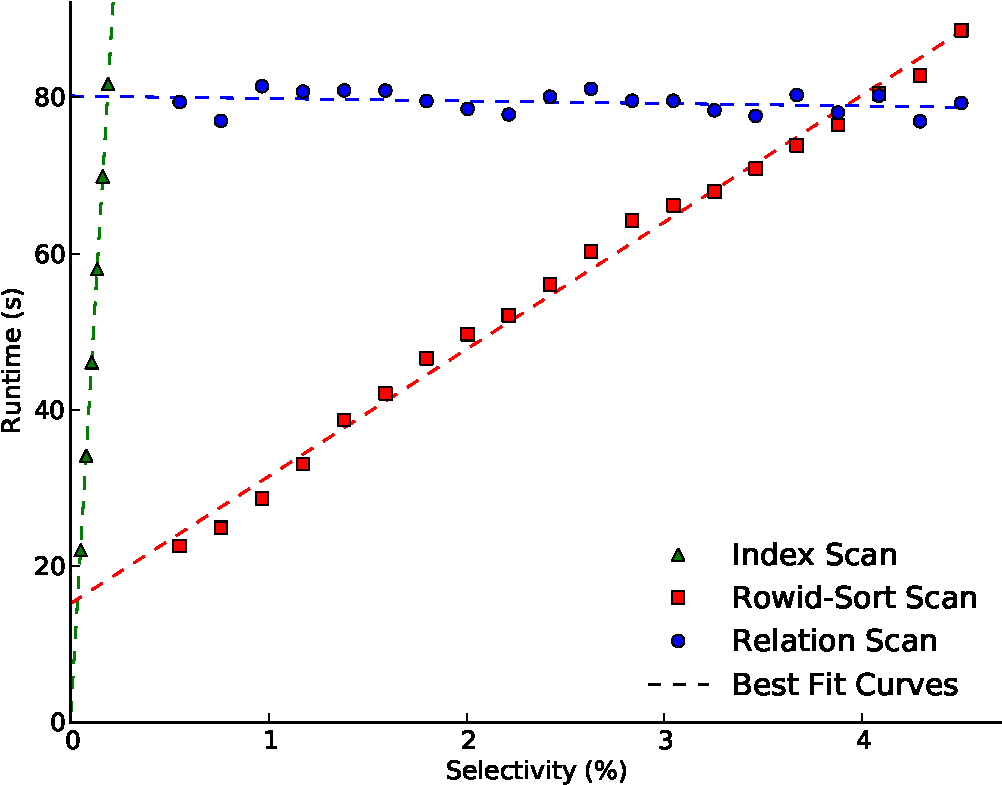
\includegraphics[width=5.0in]{FlashOpti/ScanDisk.pdf}
\caption{ \textbf{Scan operator performance on Disk.} Relation scan outperforms the alternatives at selectivities above 4\%, while index scan is optimal only for vanishingly small selectivities (e.g., single-tuple queries).  Best fit curves drawn for convenience.}
\label{fig:scan-disk}
%}
%\hspace{0.5in}
\end{figure*}
\begin{figure*}
\centering
%\subfigure[Flash SSD.]{
  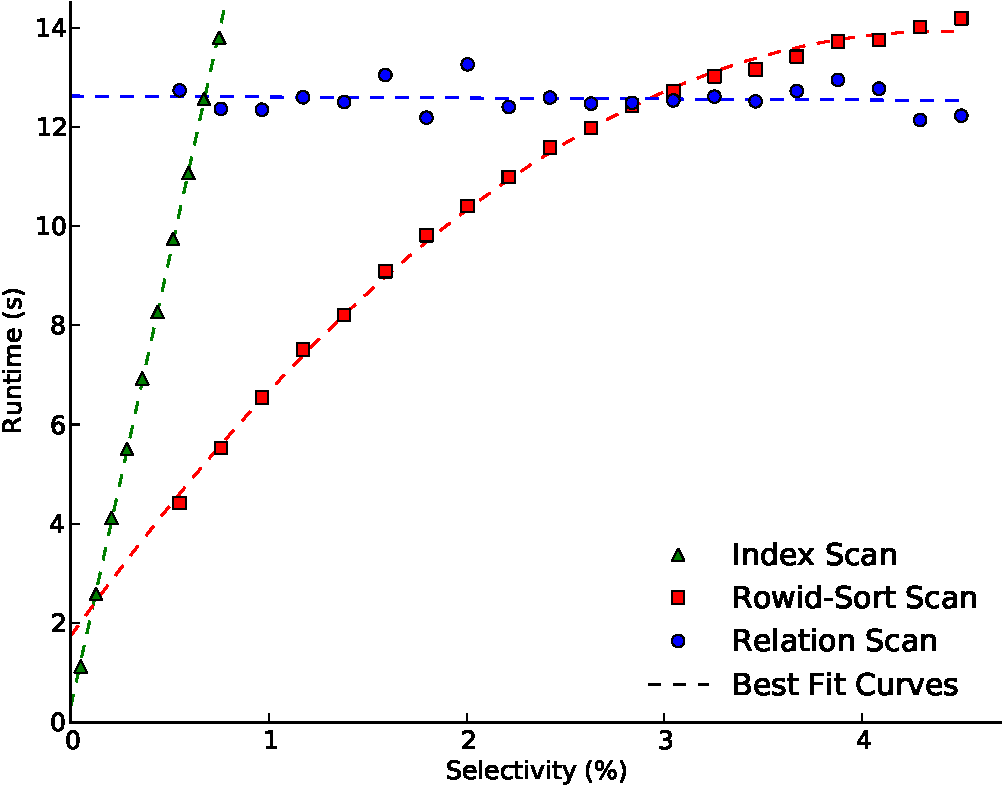
\includegraphics[width=5.0in]{FlashOpti/ScanFlash.pdf}
%}
\caption{ \textbf{Scan operator performance on Flash SSD.} Though both break-even points shift as our intuition suggests, the selectivities where the optimal decision differs between Disk and SSD are so narrow that the difference is inconsequential in practice.  Best fit curves drawn for convenience.}
\label{fig:scan-ssd}
\end{figure*}

I compare the measured performance of the different scan operators as a function of selectivity on SSD and disk.
The objective is to find the break-even points where the optimal scan operator shifts from index scan to rowid-sort scan and finally to relation scan on each device, and the performance impact in regions where this decision differs.
I issue queries for ranges of tuples using a uniformly distributed integer field on a table with 10 million rows, or roughly 2 GB. 
I use a pipelined aggregation function to ensure that no output table is materialized.

Figures~\ref{fig:scan-disk} and~\ref{fig:scan-ssd} report scan runtime on disk and Flash SSD, respectively.
The figures show the measured runtime of each scan (in seconds); lower is better. 
Recall from Section~\ref{sec:FlashOpti:Intro} that classic rules of thumb suggest that, on disk, the break-even point between index and relation scan should occur near 10\% selectivity, and intuition suggests an even higher break-even point for SSD.
Clearly, the conventional wisdom is flawed even for rotating disks; relation scan dominates above selectivities of just 4\% (the trends shown in the figure continue to the right).  
In the intermediate range from about 0.1\% to 4\% selectivity the rowid-sort scan performs best.

However, the more important analysis is to compare the locations of the break-even points across SSD and disk.  
Both crossover points shift in the expected directions.
The slope of the index scan curve is considerably shallower, and the break-even with the relation scan shifts above 0.5\% selectivity.  
Furthermore, the range in which rowid-sort scan is optimal becomes narrower.
Nevertheless, the key take-away is that the range of selectivities for which the optimal scan \emph{differs} across SSD and Disk is vanishingly small.
Only a minute fraction of queries fit into this range, and queries that make the incorrect decision (between disk and Flash) see a small performance impact.
Hence, it is unnecessary for the optimizer to be SSD-aware to choose an effective scan operation.

Whereas these measurements demonstrate my main result, they do not explain why index scans fail to leverage the random access advantage of Flash.  
I turn to this question next. 

\textbf{Analytic results.}
\begin{figure*}
\centering
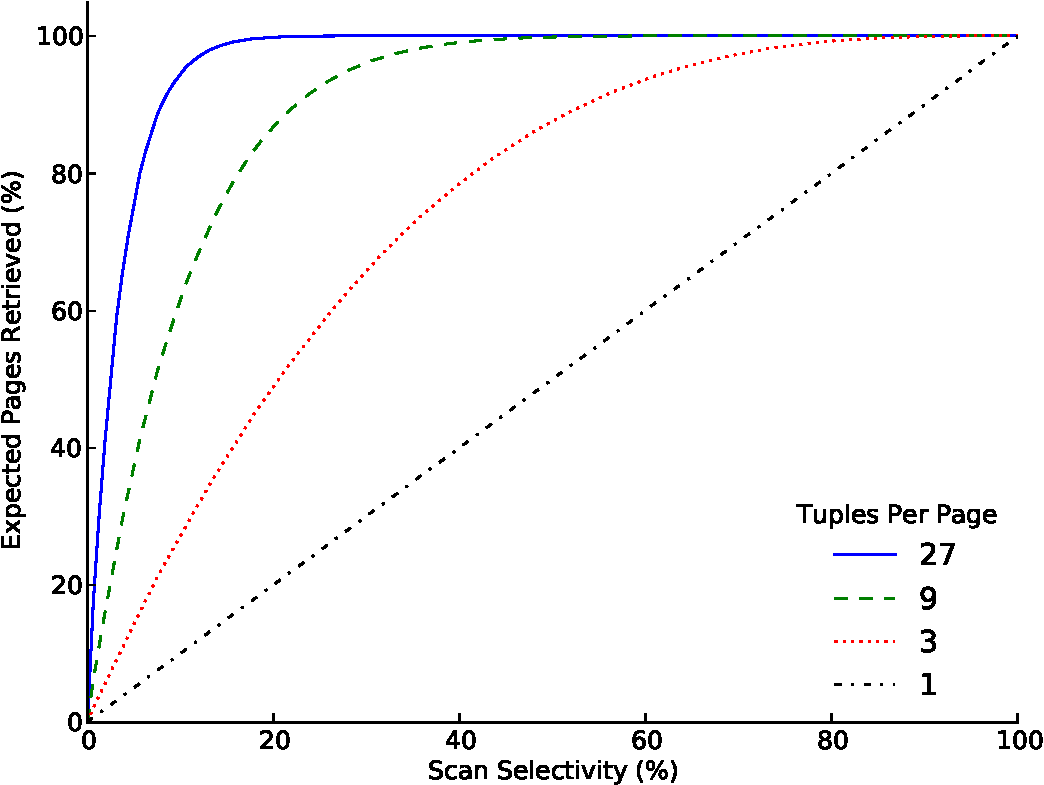
\includegraphics[width=5.0in]{FlashOpti/expectedPagesRet.pdf}
\caption{Index scans touch the majority of pages even at low selectivities.}
\label{figure::analyticScan}
\end{figure*}

The previous results show that index scan underperforms at selectivities far below what the classic 10\% rule of thumb suggests. 
The flaw in the conventional wisdom is that, when there are many tuples per page, the vast majority of \emph{pages} need to be retrieved even if only a few \emph{tuples} are accessed.
When the 10\% rule is applied to page- rather than tuple-selectivity, the guideline is more reasonable.
Yue \emph{et al.} provide an analytical formula for the expected number of pages retrieved given the size of the table, tuples per page, and selectivity \cite{Yue1975}, assuming tuples are randomly distributed among pages (a reasonable assumption given that each table can be clustered on only a single key).
Based on this formula, Figure~\ref{figure::analyticScan} shows the expected percentage of pages retrieved as a function of query selectivity and tuples per page.
When a page contains only a single tuple, clearly, the number of tuples and pages accessed are equal.
However, as the number of tuples per page increases, the expectation on the number of pages that must be retrieved quickly approaches 100\% even at small selectivities.
As a point of reference, given a 4kb page size and neglecting page headers, the Wisconsin Benchmark stores 19 tuples per page while TPC-H's Lineitem and Orders tables store 29 and 30 tuples per page, respectively.

The implication of this result is that, for typical tuple sizes, the vast majority of pages in a relation must be read even if the selectivity is but a few percent.
Hence, with the exception of single-tuple lookups, there are few real-world scenarios where scan performance improves with better random access latency under conventional storage managers that access data in large blocks.
To benefit from low access latency, future devices will need to provide random access at tuple (rather than page) granularity.
Until such devices are available, relation and rowid-sort scans will dominate, with IO bandwidth primarily determining scan performance.

\section{Join Analysis}
\label{sec:FlashOpti:Joins}

I next study the variability in join performance across disk and Flash SSD.  
Again, the objective is to identify cases where the optimal join algorithm for disk consistently results in grossly sub-optimal performance on Flash SSD.
Such scenarios imply that it is important for the optimizer to be SSD aware.

DB2 implements nested loop, sort-merge, and hybrid hash join operators.  
However, DB2 does not support a block nested loop join; its nested loop join performs the join tuple-by-tuple instead of prefetching pages or other blocks, relying on indexes to provide high performance.
Hence, unless the join can be performed in memory, the nested loop grossly underperforms the other two algorithms for ad-hoc queries (those that do not use indexes) regardless of storage device and will not be selected by the query optimizer unless it is the only alternative (e.g., for inequality joins). 
I therefore restrict the investigation to a comparison of sort-merge and hybrid hash joins.

When a clustered index exists for a particular scan or join this index should almost always be used, regardless of the nature of the storage device.  
Hence, I do not include clustered indexes in my analysis.
Furthermore, I evaluate only ad hoc joins.
When indexes are available, the choice of whether or not to use the index is analogous to the choice of which scan operator to use for a simple select query, which is covered by the previous analysis of scans.

Because of the complex interplay between available memory capacity and relation sizes for join optimization \cite{DBLP:journals/vldb/HaasCLS97}, I do not have a specific expectation that one join algorithm will universally outperform another on Flash SSD as opposed to disk.
Rather, I perform a cross-product of experiments over a spectrum of relation sizes and output projectivities using the Wisconsin Benchmark database.  
Haas's model demonstrates the importance of the relative sizes of input relations and main memory capacity on join performance; hence I explore a range of joins that are only slightly larger than available memory (joining two 1.9GB tables) to those that are an order of magnitude larger (joining two 9.7GB tables).   
I vary projectivity, having discovered empirically that it significantly impacts the optimal join algorithm on disk, as it has a strong influence on partition size in hybrid hash joins.
I execute queries with two projectivities: approximately 5\% (achieved by selecting all the integer fields in the Wisconsin Benchmark schema), and approximately 25\% (selecting an integer field and one of the three strings in the schema).
In all experiments, I perform an equijoin on an integer field, and use an aggregation operator to avoid materializing the output.

\begin{figure*}
\centering
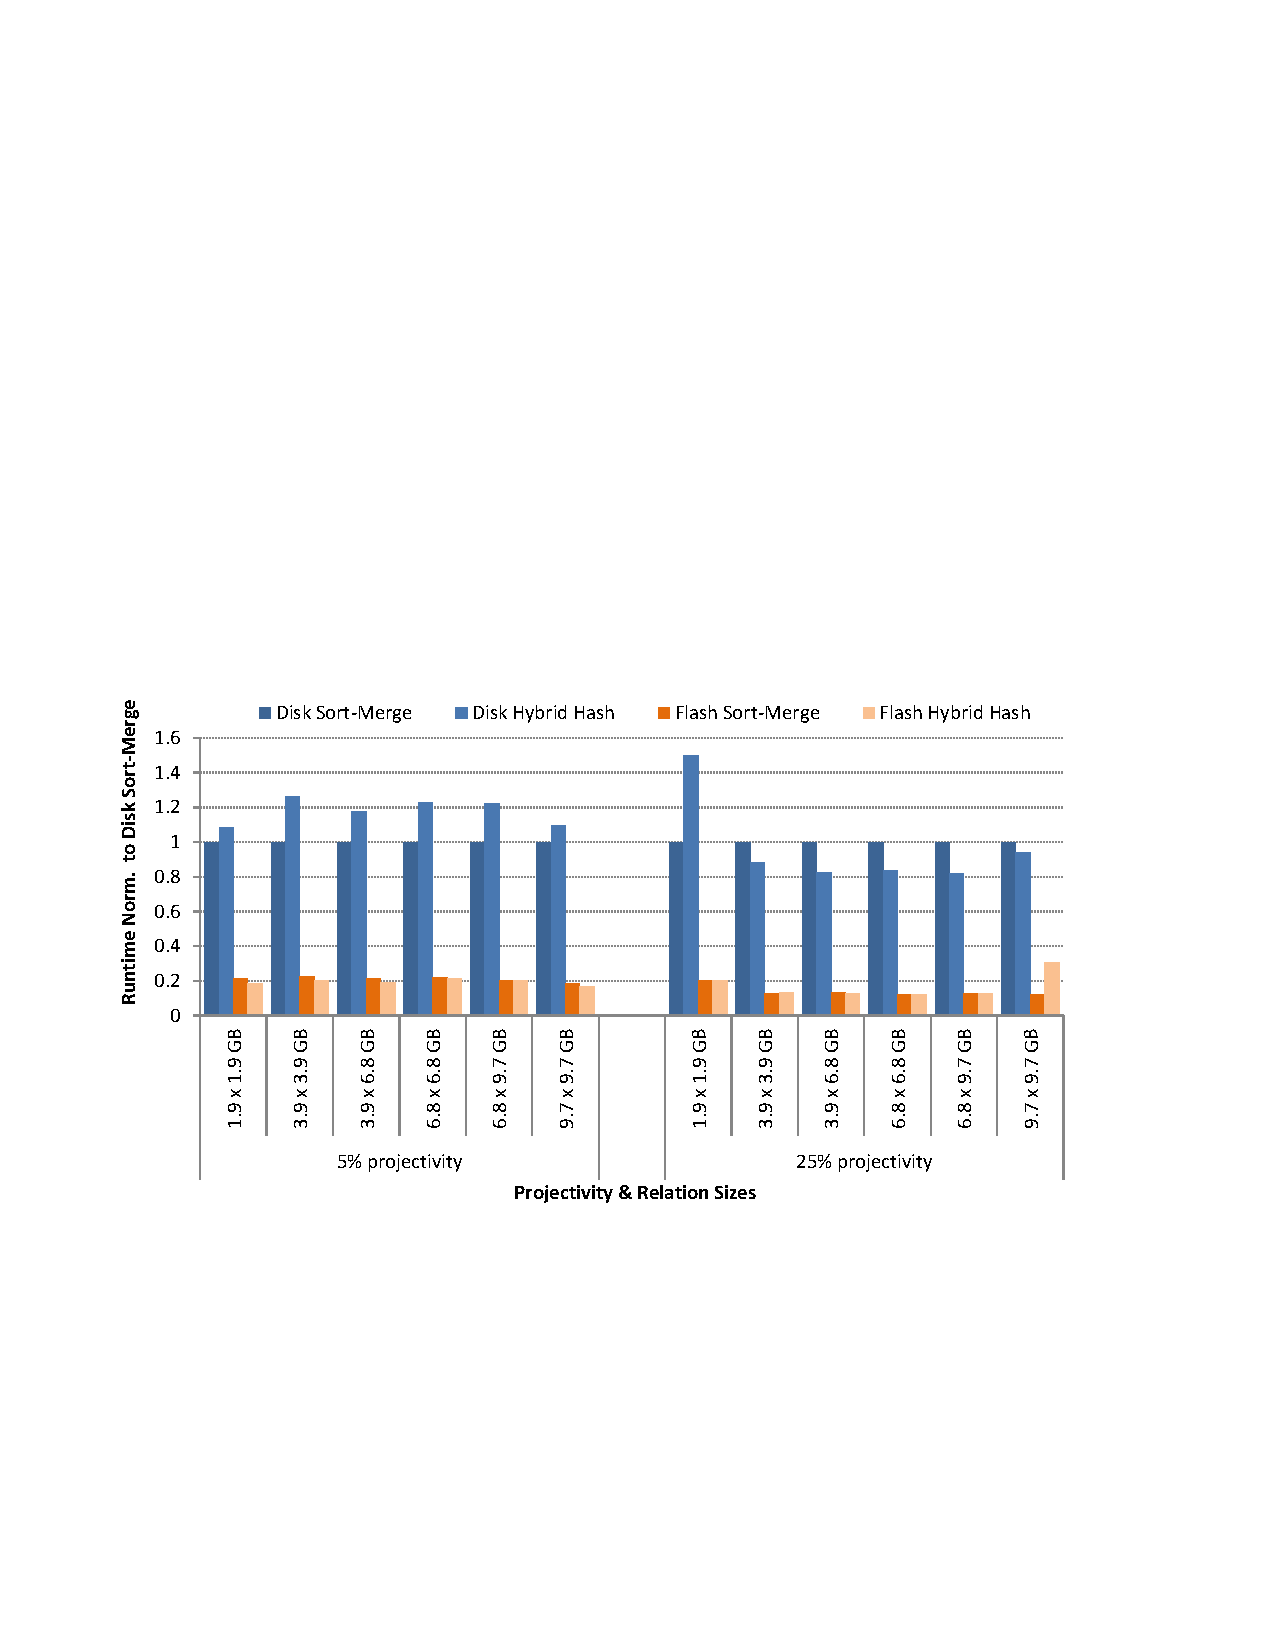
\includegraphics[width=6.0in]{FlashOpti/join.pdf}
\caption{\textbf{Join performance.}  Join runtimes on Flash SSD and Disk, normalized for each join to the runtime of sort-merge on disk.  Though there is significant variability in join algorithm performance on disk, performance variability on SSD is dwarfed by the  6\texttimes~performance advantage of moving data from disk to SSD.}
\label{figure::joins}
\end{figure*}


I report results in graphical form in Figure~\ref{figure::joins} and absolute run times in Table~\ref{table::joins}.
In Figure~\ref{figure::joins}, each group of bars shows the relative performance of sort-merge and hybrid hash joins on disk (darker bars) and Flash SSD (lighter bars), normalized to sort-merge performance on disk.
Lower bars indicate higher performance.
I provide the same data in tabular form to illustrate the runtime scaling trends with respect to relation size, which are obscured by the normalization in the graph.

Two critical results are immediately apparent from the graph.  
First, Flash SSDs typically outperform disk by 5\texttimes~to 6\texttimes~regardless of join algorithm, a margin that is substantially higher than the gap in sequential IO bandwidth, but far smaller than the gap in random IO bandwidth (see Table~\ref{table:DiskCharacteristics}).
Hence, though both join algorithms benefit from the improved random IO performance of SSDs, the benefit is muted compared to the 100\texttimes~device-level potential.
Second, whereas there is significant performance variability between the join algorithms on disk (typically over 20\%), with the exception of a single outlier, the variability is far smaller on Flash SSD (often less than 1\%).
From these results I conclude that although important on disk, the choice of sort-merge vs hybrid hash join on SSD leads to inconsequential performance differences relative to the drastic speedup of shifting data from disk to Flash.
Hence, there is no compelling reason to make the query optimizer SSD-aware; the choice it makes assuming the performance characteristics of a disk will yield near-optimal performance on SSD.

\begin{table*}
\centering
\begin{tabular}{c@{\hspace{12pt}}c@{\hspace{12pt}}c@{\hspace{12pt}}c@{\hspace{1pt}}c@{\hspace{12pt}}c@{\hspace{12pt}}c}
%\begin{tabular}{c  c | c | c | c | c}
  \toprule
	\multirow{2}{*}{Projectivity} 		      & \multirow{2}{*}{Table Sizes} & \multicolumn{2}{c}{Disk}    & &  \multicolumn{2}{c}{Flash SSD}  \\ 
\cmidrule{3-4} \cmidrule{6-7}
	 &  & Sort-merge & Hybrid hash     & &  Sort-merge & Hybrid hash  \\ 
   \midrule
5\%	& 1.9 x 1.9 GB	& 187 	& 202	& & 40		& 34	\\
	& 3.9 x 3.9 GB	& 358	& 451	& & 80		& 72	\\
	& 3.9 x 6.8 GB	& 487	& 574	& & 103	& 93	\\
	& 6.8 x 6.8 GB	& 649	& 795	& & 142	& 140\\
	& 6.8 x 9.7 GB	& 816	& 997	& & 166	& 166\\
	& 9.7 x 9.7 GB	& 1084	& 1189	& & 202	& 183\\
  \midrule
25\% & 1.9 x 1.9 GB	& 236	& 355	& & 48		& 48	\\
	& 3.9 x 3.9 GB	& 751	& 662	& & 97		& 101\\
	& 3.9 x 6.8 GB	& 947	& 781	& & 125	& 122\\
	& 6.8 x 6.8 GB	& 1415	& 1182	& & 174	& 173\\
	& 6.8 x 9.7 GB	& 1581	& 1298	& & 199	& 199\\
	& 9.7 x 9.7 GB	& 2081	& 1955	& & 250	& 634\\
  \bottomrule
\end{tabular}
\caption{\textbf{Absolute join performance.}  Join runtimes in seconds.  Variability in join runtimes is far lower on Flash SSD than on Disk.}
\label{table::joins}
\end{table*}



I highlight two notable outliers in the results.
On disk, the best join algorithm is strongly correlated to query projectivity with the exception of the 1.9GB~\texttimes~1.9GB join at 25\% projectivity.
Because the required hash table size for this join is close to the main memory capacity, I believe that this performance aberration arises due to DB2 selecting poor partition sizes for the join.
Second, on Flash, I observe a large performance difference (over 2\texttimes) between sort-merge and hybrid hash join for the largest test case, a 9.7GB~\texttimes~9.7GB join at 25\% projectivity.
For this query, I observe a long CPU-bound period with negligible IO at the end of the hybrid hash join that does not occur for any of the other hash joins.
Hence, I believe that this performance aberration is unrelated to the type of storage device, and may have arisen due to the methods employed to coax the optimizer to choose this join algorithm.
In any event, neither of these outliers outweigh the broader conclusion that there is no particular need for the query optimizer to be SSD aware.

\section{Related Work}
\label{sec:FlashOpti:RelatedWork}
Previous work studying the applicability of Flash memory in DBMS applications has focused on characterizing Flash, benchmarking specific database operations on Flash, and designing new layouts, data structures, and algorithms for use with Flash.

Both Bouganim \emph{et al.} and Chen \emph{et al.} benchmark the performance of Flash for various IO access patterns \cite{Bouganim09uflip:understanding, Chen2009}.
Bouganim introduces the uFLIP micro-benchmarks and tests their performance on several devices.
Chen introduces another set of micro-benchmarks, concluding that poor random write performance poses a significant barrier to replacing conventional hard disks with Flash SSDs.
While these micro-benchmarks are instructive for understanding database performance, I focus specifically on the performance of existing scan and join operators on SSD and disk.
Others have also benchmarked Flash's performance within the context of DBMS systems.
Lee \emph{et al.} investigate the performance of specific database operations on Flash, including multiversion concurrency control (MVCC), external sort, and hashes \cite{Lee2008}.
Similar to my study, Do \emph{et al.} benchmark ad hoc joins, testing the effects of buffer pool size and page size on performance for both disk and Flash \cite{Do2009}.
Although related to this study, neither of these works look at the specific performance differences between disk and Flash for scans and joins and how this might impact query optimization.

Whereas the above works (and this study) focus on measuring the performance of existing databases and devices, others look ahead to redesign DBMS systems in light of the characteristics of Flash.
Yin \emph{et al.} and Li \emph{et al.} present new index structures, focusing on maintaining performance while using sequential writes to update the index \cite{Yin2009, Li2009}.
Baumann \emph{et al.} investigate Flash's performance alongside a hybrid row-column store referred to as ``Grouping" \cite{Baumann2010}.
Similarly, Tsirogiannis \emph{et al.} use a column store motivated by the PAX layout to create faster scans and joins \cite{Tsirogiannis2009}.

Interestingly, my findings contradict recommendations from many of these studies.
Baumann concludes that SSDs shift optimal query execution towards index-based query plans.
The study bases this conclusion on the observation that asynchronous random reads on Flash are nearly as fast as sequential reads.
Indeed, the arguments made by Baumann are a key component of the intuition laid out in Section~\ref{sec:FlashOpti:Intro} that led me to expect a need for SSD-aware query optimization.
However, the conclusion neglects the observations discussed in Section~\ref{sec:FlashOpti:Scans} demonstrating that queries selecting more than a handful of tuples will likely retrieve the majority of pages in a relation, and thus gain no advantage from fast random IO.
Tsirogiannis introduces a join algorithm that retrieves only the join columns, joins these values, and then retrieves projected rows via a temporary index.
By the previous argument, scanning for projected data should retrieve the majority of data pages, preferring a relation scan, and thus provide comparable advantage on disk and SSD.

Finally, Bausch \emph{et al.} implement asymmetry-aware query optimization in PostgreSQL \cite{BauschPetrov12}.
They calibrate and evaluate their system using the TPC-H benchmark and find substantial improvement.
However, I believe their calibration and evaluation are skewed and lead to false conclusions (their results are insufficient to demonstrate that query optimizers should be SSD-aware).
First, their results show that an external sort of unordered data results results in 95\% random read accesses to disk.
This is indicative of poorly configured memory buffers; external soft algorithms should exhibit almost entirely sequential access patterns.
Furthermore, the results of their calibration (shown in their appendix) differ substantially from expected physical traits.
For example, the relative cost of disk's random access is only $6.8\times$ that of a sequential access, the relative cost of Flash's random read access is $5.6\times$ that of its sequential read access (nearly the same as the relative difference on disk), and Flash's sequential writes are roughly $2.5\times$ \emph{slower} than random writes (sequential writes should be faster).
Using a physically-based model only makes sense if the model is accurate.
I believe the improvement shown is a function of (1) using the total time of 21 queries as the performance and calibration metric instead of arithmetic or geometric mean (query 21 shows improvement of 549\% and has a greater runtime than most other queries), (2) using search-based calibration instead of physically derived optimization parameters (e.g., the cost of a disk seek should be measured directly from the disk, not by fitting the model), and (3) the asymmetric model has seven parameters versus the original model's five; these additional degrees of freedom allow more effective search-based calibration even when using an incorrect optimization model.
I believe that my work demonstrates fundamental principles suggesting that query optimization sees little benefit from SSD-awareness.

\section{Conclusion}
\label{sec:FlashOpti:Conclusion}
Flash-based solid state disks provide an exciting new high-performance alternative to disk drives for database applications.
My investigation of SSD-aware query optimization was motivated by a hope that the drastically improved random IO performance on SSDs would result in a large shift in optimal query plans relative to existing optimizations.
At a minimum, I expected that constants capturing relative IO costs in the optimizer would require update.
This chapter presented evidence that refutes this expectation, instead showing that an SSD-oblivious query optimizer is unlikely to make significant errors in choosing access paths or join algorithms.
Specifically, I demonstrated both empirically and analytically that the range of selectivities for which a scan operation can benefit from SSDs' fast random reads is so narrow that it is inconsequential in practice.
Moreover, measurements of alternative join algorithms reveal that their performance variability is far smaller on SSDs and is dwarfed by the 5\texttimes~to 6\texttimes~performance boost of shifting data to SSD. 
Overall, I conclude that the small and inconsistent performance gains available by making query optimizers SSD-aware are not worth the effort.


 \chapter{Architecting Recovery Management for NVRAM}
 \label{chap:OLTP_design}
 The following two chapters consider the impact of using emering NVRAM technologies for durable transaction processing.
Refer to Section~\ref{sec:Background:Storage:NVRAM} for an overview of storage technologies and Section~\ref{sec:Background:Recovery} for a description of ARIES, a popular recovery mechanism for disk.
Work relating to the next two chapters is currently under review at VLDB.
I completed this work under the advisement of my advisor, Thomas F. Wenisch, and collaborators at Oracle, Brian T. Gold and Bill Bridge.
I was the sole graduate student and technical contributer (programming and running experiments) for the project, although my co-authors were vital to development the following ideas.
I would especially like the thank Brian and Bill for bringing industry's point of view and ``real world" examples to this collaboration.

This chapter outlines the problems with existing disk recovery management, the potential pitfalls of using NVRAM for persistent applications, a methodology for evaluating NVRAM devices that do not yet exist, and a description of several candidate software designs for NVRAM recovery management, to be evaluated later.
I consider this chapter largely complete with two exceptions.
First, I have performed a validation of my timing model that has not yet been published that I intend to include in the final thesis \ref{sec:OLTP_design:Methodology:Proposed}.
Second, my implementation of \GroupCommit is more complex (and interesting, in my opinion) than a 12 page journal paper allows room to describe.
I intend to include a detailed description in Section~\ref{sec::OLTP_design:GroupCommit:Proposed}.

\section{Introduction}
\label{sec:OLTP_design:Intro}

Emerging nonvolatile memory technologies (NVRAM) offer an alternative to disk that is persistent, provides read latency similar to DRAM, and is byte-addressable \cite{BurrKurdi08}.
Such NVRAMs could revolutionize online transaction processing (OLTP), which today must employ sophisticated optimizations with substantial software overheads to overcome the long latency and poor random access performance of disk.
Nevertheless, many candidate NVRAM technologies exhibit their own limitations, such as greater-than-DRAM latency, particularly for writes \cite{LeeIpek09}.

These NVRAM technologies stand to revolutionize Online Transaction Processing (OLTP), where consistency and durability are paramount, but applications demand high throughput and low latency.
Prior work has already demonstrated the potential of these technologies to enhance file systems \cite{GreenanMiller06, ConditNightingale09} and persistent data structures \cite{VenkataramanTolia11}, but has not considered OLTP. 
Today, OLTP systems are designed from the ground up to circumvent disk's performance limitations.
For example, many popular database systems use Write-Ahead Logging (WAL; e.g., ARIES \cite{MohanHaderle92}) to avoid expensive random disk writes by instead writing to a sequential log.  
Although effective at hiding write latency, WAL entails substantial software overheads.

NVRAM offers an opportunity to simultaneously improve database forward-processing throughput and recovery latency by rethinking mechanisms that were designed to address the limitations of disk.
Figure~\ref{fig::Recovery} demonstrates this potential, displaying recovery time and transaction throughput for the TPCB workload running on the Shore-MT storage manager \cite{JohnsonPandis09} for hypothetical NVRAM devices (see Section~\ref{sec:OLTP_design:Methodology} for a description of the methodology).

\begin{figure}
  \centering
  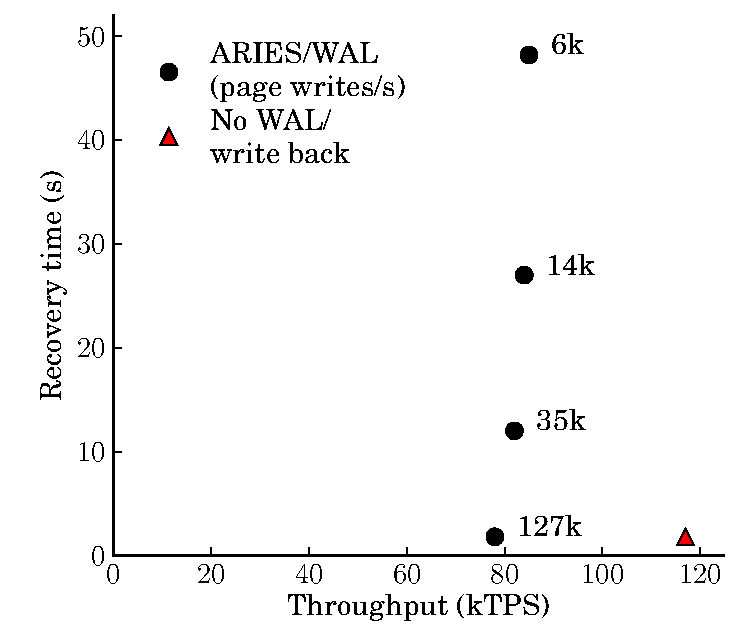
\includegraphics[width=.6\linewidth]{OLTP_design/TPCB_Recovery.pdf}
  \caption{\textbf{TPCB recovery latency vs throughput.} Increasing page flush rate reduces recovery latency.  Removing WAL entirely improves throughput by 50\%.}
  \label{fig::Recovery}
\end{figure}


The ARIES/WAL points (black circles) in the Figure show forward-processing throughput (horizontal axis) and recovery time (vertical axis) as a function of device write throughput (annotated alongside each point).
As database throughput can greatly outpace existing storage devices (this configuration requires 6,000 page writes/s to bound recovery at maximum transaction throughput; measured disk and flash devices provide only 190 and 2,500 page writes/s, respectively) I model recovery performance under faster NVRAM using a RAM disk for log and store while limiting the page flush rate.
As intuition would suggest, greater write bandwidth enables more aggressive flushing, minimizing the number of dirtied pages in the buffer cache at the time of failure, reducing recovery time.
With enough write bandwidth (in this case, 127,000 flushes/s, or 0.97 GB/s random writes for 8KB pages) the database recovers near-instantly, but forward-processing performance remains compute bound.
Achieving such throughput today requires large, expensive disk arrays or enterprise flash storage devices; future NVRAM devices might enable similar performance on commodity systems.

NVRAM opens up even more exciting opportunities for recovery management if we consider re-architecting database software.
The Figure shows this additional potential with a design point (red triangle) that removes WAL and asynchronous page flushing---optimizations primarily designed to hide disk latency.
Throughput improves due to three effects: (1) threads previously occupied by page and log flushers become available to serve additional transactions, (2) asynchronous page flushing, which interferes with transactions as both flusher and transaction threads latch frequently accessed pages, is removed, and (3) transactions no longer insert WAL log entries, reducing the transaction code path.
In aggregate these simplifications amount to a 50\% throughput increase over ARIES's best possible NVRAM performance.
The key take-away is that database optimizations long used for disk only hinder performance with faster devices.
In this chapter, I investigate how to redesign durable storage and recovery management for OLTP to take advantage of the low latency and byte-addressability of NVRAM.

NVRAMs, however, are not without their limitations.
Se\-veral candidate NVRAM technologies exhibit larger read latency and significantly larger write latency compared to DRAM.
Additionally, whereas DRAM writes benefit from caching and typically are not on applications' critical paths, NVRAM writes must become persistent in a constrained order to ensure correct recovery.
I consider an NVRAM access model where correct ordering of persistent writes is enforced via \emph{persist barriers}, which stall until preceding NVRAM writes are complete; such persist barriers can introduce substantial delays when NVRAM writes are slow.

This chapter outlines an approach to architecting recovery management for transaction processing using NVRAM technologies
I discuss potential performance problems with using NVRAM and possible software architectures to address these problems.
Additionally, I propose an evaluation framework, involving memory trace analysis, code annotation, and precise timing models for OLTP running on existing hardware platforms.
Subsequent chapters will build on the designs and methodology presented here to determine when OLTP must be redesigned and what problems might remain.

\section{Recovery Management Design}
\label{sec:OLTP_design:Design}

\begin{table*}
  \footnotesize
  \centering
  \renewcommand{\arraystretch}{2.5}
  \begin{tabular*}{\textwidth}{l l l l}
     & \pbox{1.1 in}{\emph{NVRAM\newline Disk-Replacement}} & \pbox{1.5 in}{\InPlace} & \pbox{1.5 in}{\GroupCommit} \\
    \emph{Software buffer} & \cellcolor[gray]{.8}\pbox{1.1 in}{Traditional WAL/ARIES} & \cellcolor[gray]{.8}\pbox{1.5 in}{Updates both buffer and NVRAM} & \cellcolor[gray]{.8}\pbox{1.5 in}{Buffer limits batch size} \\
    \emph{Hardware buffer} & \cellcolor[gray]{.95}\pbox{1.1 in}{Impractical} & \cellcolor[gray]{.95}\pbox{1.5 in}{Slow uncached NV\-RAM reads} & \cellcolor[gray]{.95}\pbox{1.5 in}{Requires hardware support} \\
    \emph{Replicate to DRAM} & \multicolumn{3}{l}{\pbox{4.1 in}{\cellcolor[gray]{.8}Provides fast reads and removes buffer management, but requires large DRAM capacity}} \\
  \end{tabular*}
  \caption{\textbf{NVRAM design space.} Database designs include recovery mechanisms (top) and cache configurations (left).}
  \label{table::DesignSpace}
\end{table*}


Near-future NVRAM devices will undoubtedly be faster than both disk and flash.
However, compared to DRAM many NVRAM technologies impose slower reads and significantly slower persistent writes.
We must consider both in redesigning OLTP for NVRAM.

\subsection{NVRAM Reads}
\label{sect:OLTP_design:Design:Reads}
While the exact read performance of future NVRAM technologies is uncertain, many technologies and devices increase read latency relative to DRAM.
Current databases and computer systems are not equipped to deal with this read latency.
Disk-backed databases incur sufficiently large read penalties (on the order of milli-seconds) to justify software-managed DRAM caches and buffer management.
On the other hand, main-memory databases rely only on the DRAM memory system, including on-chip data caches.
Increased memory latency and wide-spread data accesses may require hardware or software-controlled DRAM caches even when using byte addressable NVRAM.

I consider three configurations of cache management; these alternatives form the three rows of Table~\ref{table::DesignSpace} (subsequent sections consider the recovery management strategies, forming the three columns).
The first option, \emph{Software Buffer}, relies solely on software to manage a DRAM buffer cache, as in conventional disk-backed database systems.
The cache may be removed entirely or execution relies soly on a \emph{Hardware Buffer}, as in main-memory databases.
Hardware caches are fast (e.g., on-chip SRAM) and remove complexity from the software, but provide only limited capacity.
Third, one might \emph{replicate to DRAM} all data that is stored in NVRAM---all writes update both DRAM and NVRAM (for recovery), but reads retrieve data exclusively from DRAM.
Replicating data ensures fast reads by avoiding increased NVRAM read latencies (except for recovery) and simplifies buffer management, but requires large DRAM capacity.

\subsection{NVRAM Writes}
\label{sec:OLTP_design:Design:Writes}

Persistent writes, unlike reads, do not benefit from cach\-ing; writes persist through to the device for recovery correctness.
Additionally, NVRAM updates must be carefully ordered to ensure consistent recovery.
I assume that ordering is enforced through a generic mechanism called a \emph{persist barrier}, which guarantees that writes before the barrier persist before any dependant operations after the barrier persist.

Persist barriers may be implemented in several ways.
The easiest, but worst performing, is to delay threads that issue persist barriers until all pending NVRAM writes successfully persist.
More complicated mechanisms improve performance by allowing threads to continue executing beyond the persist barrier and only delaying thread execution when persist conflicts arise (i.e., a thread reads or overwrites shared data from another thread that has not yet persisted).
BPFS provides an example implementation of this mechanism \cite{ConditNightingale09}.
Regardless of how they are implemented, persist barriers can introduce expensive synchronous delays on transaction threads; the optimal recovery mechanism depends on how expensive, on average, persist barriers become.
To better understand how persist barriers are used and how frequently they occur, I outline operations to atomically update persistent data using persist barriers, and use these operations to implement three recovery mechanisms for NVRAM.

\textbf{Atomic durable updates.}
{
\singlespacing
\newsavebox{\persistwal}
\begin{lrbox}{\persistwal}
\begin{lstlisting}
persist_wal(log_buffer, nvram_log)
  for entry in log_buffer:
    nvram_log.force_last_lsn_invalid(entry)
    nvram_log.insert_body(entry) # no lsn
  persist_barrier()
  nvram_log.update_lsns()
  persist_barrier()
\end{lstlisting}
\end{lrbox}

\newsavebox{\persistpage}
\begin{lrbox}{\persistpage}
\begin{lstlisting}
persist_page(page_v, page_nv, page_log)
  page_log.copy_from(page_nv)
  persist_barrier()
  page_log.mark_valid()
  persist_barrier()
  page_nv.copy_from(page_v)
  persist_barrier()
  page_log.mark_invalid()
  persist_barrier()
\end{lstlisting}
\end{lrbox}

\begin{figure}[]
  \subfigure{ \usebox{\persistwal} }
  \subfigure{ \usebox{\persistpage} }

  \caption{\textbf{Durable atomic updates.} \texttt{persist\_wal()} appends to the ARIES log using two persist barriers.  \texttt{persist\_page()} persists pages with four persist barriers.}
  \label{fig::Code}
\end{figure}
}

Figure~\ref{fig::Code} shows two operations to atomically update NVRAM data.
The first, \texttt{persist\_wal()}, persists log entries into an ARIES log.
Sho\-re-MT log entries are post-pended with their Log Serial Number (LSN -- log entry file offset).
At recovery, a log entry is considered valid only if this tail LSN matches the location of the entry.
I persist log entries atomically by first persisting an entry without its tail LSN, and only later (once we are certain the entry is persistent) persist the LSN.
This order is enforced by inserting a persist barrier between writing the log entry and its LSN.
Additionally, I reduce the number of persist barriers by persisting entries in batches, writing several log entries at once (without LSNs), followed by all their LSNs, separated by a single persist barrier.
It is entirely possible (yet unlikely) that pre-existing LSN tails already match the log entry's offset; tails must be checked and first reset when this occurs.
Log operations introduce two persist barriers---one to ensure that log entries persist before their LSNs, and one to enforce that LSNs persist before the thread continues executing.

The second operation, \texttt{persist\_page()}, atomically persists page data with the use of a persistent undo page log.
First, the page's original data is copied from NVRAM to the page log.
The page log is marked valid and the dirty version of the page is copied to NVRAM (or updated in-place while locks are held).
Finally, the log is marked invalid.
Four persist barriers ensure that each update persists before the next, enforcing consistency at all points in execution.
Recovery checks the valid flags of all page logs, copying any valid log back in-place.
The log is always valid while the page persists in-place, protecting against partial NVRAM writes.
Together, \texttt{persist\_wal()} and \texttt{persist\_page()} provide the tools necessary to construct recovery mechanisms.
I discuss these mechanisms next, describing their implementation and performance.

\textbf{NVRAM Disk-Replacement.}
NVRAM database systems will likely continue to rely on ARIES/WAL at first, using NVRAM as \NVDisk.
WAL provides recovery for disk by keeping an ordered log of all updates, as described in Section~\ref{sec:Background:Recovery}.
While retaining disk's software interface, NVRAM disk accesses are implemented as copies between the volatile and nonvolatile address spaces.
\NVDisk in Shore-MT persists the log and pages with \texttt{persist\_wal()} and \texttt{persist\_page()}, respectively.
However, persists occur on log and page flusher threads, and transaction threads do not observe persist barrier delays (except when waiting for commit log entries to persist).
\NVDisk provides low recovery latency by aggressively flushing pages, minimizing the size of data to recover.
While requiring the least engineering effort, \NVDisk contains large software overheads to maintain a centralized log and asynchronously flush pages.
Next, I leverage NVRAM's low latency to reduce these overheads.

\textbf{In-Place Updates.}
Fast, byte-addressable NVRAM allows updates to persist in-place and enforce persist order immediately, a design we call \InPlace.
\InPlace allows us to remove the centralized log by replacing redo and undo log functionality elsewhere.
I remove redo logs by keeping the database's durable state up-to-date.
In ARIES terms, the database is constantly at its replayed state---there is no need to replay a redo log after failure.
Undo logs need not maintain a global order (transactions are already free to roll back in any order), and instead I distribute ARIES undo logs per transaction.
Such non-concurrent logs are simpler and impose less overhead than centralized logs.
Other databases (such as Oracle) already distribute undo logs in rollback segments and undo table spaces \cite{OracleDoc}.
Transaction undo logs remain durable so that in-flight transactions at the time of failure can be rolled back.
Each page update consists of (1) latching the page, (2) inserting an undo entry into the transaction-private undo log, using \texttt{persist\_wal()}, (3) updating the page in-place, using \texttt{persist\_page()} (without an intermediate volatile page), and (4) releasing the page latch.
This protocol ensures all updates to a page, and updates within a transaction, persist in-order, and that no transaction reads data from a page until it is durable.
Recovery applies undo logs for in-flight transactions; there is no need to replay a redo log.

Persisting data in-place removes expensive redo logging and asynchronous page flushing, but introduces persist barriers on transactions' critical paths.
For sufficiently short persist barrier delays \InPlace outperforms \NVDisk (if persist barrier delays are negligible \InPlace resembles existing non-recoverable in-memory databases).
However, one would expect transaction performance to suffer as persist barrier delay increases.

In response, I introduce \GroupCommit, a recovery mechanisms designed to minimize the frequency of persist barriers while still removing WAL.
\GroupCommit is an entirely new design, committing instructions in large batches to minimize persist synchronization.
The next section describes, in detail, the operation and data structures necessary to implement \GroupCommit.

\section{NVRAM Group Commit}
\label{sec:OLTP_design:GroupCommit}

The two previous recovery mechanisms provide high throughput under certain circumstances, but also fail to perform in others.
\NVDisk is insensitive to large persist barrier delays as it was originally designed for disk.
However, it assumes IO delays to be the dominant performance bottleneck and trades off software overhead to minimize IO.
\InPlace, on the other hand, excels when persist barriers delays are short.
As persist barrier latency increases performance suffers, such that \NVDisk eventually performs better.
Here, I provide a third option, coupling \NVDisk's persist barrier latency-insensitivity with \InPlace's low software overhead: \GroupCommit.

\subsection{Operating Principles and Implementation}
\label{sec:OLTP_design:GroupCommit:Proposed}

\GroupCommit operates by executing transactions in batches, whereby all transactions in the batch commit or (on failure) all transactions abort.
Transactions quiesce between batches, allowing only transactions from the oldest batch to execute.
Each transaction maintains a private ARIES-style undo log, supporting abort and roll-back as in \InPlace, but transaction logs are no longer persistent.
ARIES undo logs support concurrent durable transactions.
As batches persist atomically, transactions no longer roll back selectively during recovery, obviating the need for persistent ARIES undo logs.
Instead, recovery relies on a database-wide undo log and staging buffer to provide durable atomic batches.

\GroupCommit limits persist barrier frequen\-cy by enforcing persistence by batch rather than by transaction.
Persisting a batch resembles \texttt{persist\_page()}, used across the entire database, once per batch.
Because undo logging is managed at the batch level, transactions' updates may not persist in-place to NVRAM until all transactions in the batch complete.
Rather, transactions write to a volatile staging buffer, tracking dirtied cache lines in a concurrent bit field.
The bit field facilities quickly finding all dirtied data at batch completion.
Once the batch ends and all transactions complete, the pre-batch version of dirtied data is copied to the database-wide persistent undo log, only after which is data copied from the staging buffer in-place to NVRAM.
Finally, the database-wide undo log is invalidated, transactions commit, and transactions from the next batch begin executing.
%Batching allows NVRAM persists to coalesce -- the log persists only the earliest version of data from the batch, while only the last version of data persists in-place, with intermediate values never persisting.
On failure the log is copied back to the NVRAM database, aborting and rolling back all transactions from the in-flight batch.
The key observation is that \GroupCommit persists entire batches of transactions using four persist barriers, far fewer than required with \InPlace.  Note, however, that it enables recovery only to batch boundaries, rather than transaction boundaries.

I briefly outline two implementation challenges: long transactions and limited staging buffers.
Long transactions present a problem by forcing all other transactions in the batch to defer committing until the long transaction completes.
Limited staging buffers, not large enough to fit the entire data set, may fill while transactions are still executing.
I solve both problems by resorting to persistent ARIES-style undo logs, as in \InPlace.
Long transactions persist their ARIES undo log (previously volatile), allowing the remainder of the batch to persist and commit.
The long transaction joins the next batch, committing when that batch commits.
At recovery the most recent batch rolls back, and the long transaction's ARIES undo log is applied, removing updates that persisted with previous batches.
Similarly, if the staging buffer fills, the current batch ends immediately and all outstanding transactions persist their ARIES undo logs.
The batch persists, treating any in-flight transactions as long transactions, reassigning them to the next batch.
Transaction-local ARIES undo logs invalidate as the batch commits, requiring additional persistent data structures to allow transaction and batch logs to invalidate atomically.

\GroupCommit requires fewer persist barriers than \InPlace yet avoids expensive logging found in \NVDisk.
A batch requires only four persist barriers, regardless of batch length.
Expensive persist barrier delays can be amortized over additional transactions by increasing batch length, improving throughput.
Batch length must be at least large enough to amortize time spent quiescing transactions between batches.
However, increasing batch length defers commit for all transactions in the batch, increasing transaction latency.

\subsection{Proposed Work}
\label{sec::OLTP_design:GroupCommit:Proposed}

\GroupCommit only improves throughput so long as the time between batches to quiesce transactions, locate dirtied data, and persist that data is substantially less than time during each batch where transactions execute.
To provide a fair comparison between recovery mechanisms, I implement a true version of \GroupCommit in Shore-MT.
Whereas I expect NVRAM to have sufficient bandwidth to persist data quickly, orchestrating data copies, tracking dirty data with low overhead, and locating dirty data efficiently proved to be difficult software problems.
The details of this implementation were omitted from the VLDB submission, but are included here, including work to be done.

\textbf{Concurrent Dirty Set.}
As described previously, \GroupCommit requires each batch to track dirty data.
This is done with an efficient concurrent set, tracking the set of buffer pool cache lines dirtied by each batch.
In order to maximize transaction throughput, this set must allow low overhead updates by concurrent threads during batch execution, and fast iteration during batch persist.

The first attempt to create a set used an STL \emph{ordered\_set} (implemented as a balanced tree).
However, inserting cache lines to the dirty set was prohibitively expensive, slowing transactions down.
On the other hand, \emph{ordered\_set} allows relatively fast iteration over the dirty set during batch copy.
The next attempt used a bitmap of dirty cache lines, each bit corresponding to a cache line in the buffer pool.
A 10GB buffer pool requires 20MB of bits to track dirty cache lines.
Before each batch starts, after the previous batch finishes persisting, dirty bits must be flash cleared in order to track the next batch.
While bits can be quickly updated via an atomic OR operation, iterating over the dirty bits during persist was too slow, requiring a different solution.

Instead, I leveraged the fact that dirty regions were rare and sparsely located throughput the buffer pool.
Batches contain up to thousands of transactions, yet these transactions could only manage to write to a small portion of a 10GB buffer pool.
It is therefore necessary to efficiently skip over large regions of clean data when iterating through the dirty set.
To achieve this, I created a \emph{tiered bitfield set}.
The tiered bitfield set contains two bitfield sets.
The first is as described above, where each bit corresponds to a cache line in the buffer pool.
In addition, there is a higher level bit field, each bit corresponding to a \emph{cache line of the primary bit field}.
Thus, a set bit in the top level bit field indicates that some bit within a cache line of the primary bit field is set, which in turn corresponds to dirty cache line in the buffer pool.

Updating this set requires atomic OR on the necessary bits in both bit fields of the set, a small cost.
Iterating over the set now involves iterating over the (much smaller) top level bit field, finding \emph{segments} of the primary bit field known to contain at least one set bit.
This iteration reduces both the number of instructions and cache/memory lines accessed, minimizing persist time between batches.

I propose to include additional work demonstrating the sparse nature of writes to the buffer pool, as well as timing results that show that fast dirty line tracking and persist is possible.

\textbf{Concurrent Persist.}
I have shown that dirty lines can be tracked and iterated over efficiently.
However, persisting each batch with the batch coordinator alone results in long persist delays.
These delays are due to the \emph{software} overhead of copying data, not from NVRAM limitations.
To reduce these delays all persist operations must be parallelized across threads.
Luckily, we have threads to spare -- transaction threads that have quiesced between batches.
Instead of sitting idle, these threads now participate in persisting each batch.

The buffer pool address space and corresponding portions of the dirty line set are partitioned into several segments, each placed in a task queue.
The batch coordinator and transaction threads blocked by the persist process each participate by accepting tasks to persist buffer pool partitions (both log and then data in-place).
Once all tasks complete the batch commits, allowing the next batch to begin.

I propose to include results showing that persist parallelization is necessary, but is an effective way to accelerate batching.

Once both of these optimizations are implemented the system is using all cores to persist, and profiling shows that \emph{memcpy} operations, copies from the buffer pool to the persistent address space, are the primary bottleneck (memcpy is implemented using fast SSE instructions and cannot be optimized further).
Persist time is minimized, and there is little room left for improvement.

\section{Design Space}
\label{sec:OLTP_design:Designs}
I describe the space of possible designs given choices regarding NVRAM read and write performance.
This discussion ignores possible uses of hard disk to provide additional capacity.
Each design works alongside magnetic disk with additional buffer management and the constraint that pages persist to disk before eviction from NVRAM.

Table~\ref{table::DesignSpace} lists the possible combinations of caching architectures and recovery mechanisms.
The left column presents \NVDisk, which we see as the obvious and most incremental use for NVRAM.
Of note is the center-left cell, \NVDisk without the use of a volatile buffer.
WAL, by its design, allows pages to write back asynchronously from volatile storage.
Removing the volatile cache requires transactions to persist data in-place, but do so only after associated log entries persist, retaining the software overheads of \NVDisk as well as the frequent synchronization in \InPlace.
Thus, this design is impractical.

The middle-column recovery mechanism, \InPlace, represents the most intuitive use of NVRAM in database systems, as noted in several prior works.
Agrawal and Jagadish explore several algorithms for atomic durable transactions with an NVRAM main-memory \cite{AgrawalJagadish89}.
They describe the operation and correctness of each mechanism and provide an analytic cost model to compare them.
Their work represents the middle column, middle row of Table~\ref{table::DesignSpace} (\InPlace with no volatile buffer).
Aky\"{u}rek and Salem present a hybrid DRAM and NVRAM buffer cache design alongside strategies for managing cache allocation \cite{SalemAkyrek95}.
They evaluate their allocation strategies using database traces and queuing models to demonstrate the effectiveness of NVRAM at accelerating persistent writes.
Partial Memory Buffers is closest to the middle-top cell of the design space table (\InPlace with a software-managed DRAM buffer), although that design considers NVRAM as part of a hybrid buffer, not the primary persistent store.
None of these works considers alternative approaches (such as \GroupCommit), to account for large persist barrier latency and associated delays.
Additionally, This work extends prior work by providing a more precise performance evaluation and more detailed consideration of NVRAM characteristics.

The right column presents \GroupCommit.
I am not aware of any previous work that extends disk group commit to reduce the frequency of NVRAM persist barriers.
A limited-capacity staging buffer (i.e., one insufficient for the entire data set) may limit batch size, as described above.

Each of the three recovery mechanisms may replicate all data between NVRAM and DRAM to ensure fast read accesses, manage a smaller DRAM buffer cache, or omit the cache altogether.
In Section~\ref{sec:OLTP_eval:Reads} I consider the importance of NVRAM caching to transaction throughput.
Then, in Section~\ref{sec:OLTP_eval:Persists} I assume a DRAM-replicated data store to isolate read performance from persist performance in evaluating each recovery mechanisms's ability to maximize transaction throughput.
The next section describes an evaluation methodology for OLTP on NVRAM.

\section{Methodology}
\label{sec:OLTP_design:Methodology}

This section details the methodology for benchmarking transaction processing and modeling NVRAM performance.
Experiments use the Shore-MT storage manager \cite{JohnsonPandis09}, including the high performance, scalable WAL implementation provided by Aether \cite{JohnsonPandis10}.
While Aether provides a distributed log suitable for multi-socket servers, the distributed log exists as a fork of the main Shore-MT project.
Instead, I limit experiments to a single CPU socket to provide a fair comparison between WAL and other recovery schemes, enforced using the Linux \emph{taskset} utility.
Experiments place both the Shore-MT log and volume files on an in-memory \emph{tmpfs}, and provide sufficiently large buffer caches such that all pages hit in the cache after warmup.
The intent is to allow the database to perform data accesses at DRAM speed and introduce additional delays to model NVRAM performance.
Table~\ref{table::Specs} shows the experimental system configuration.

\begin{table}
  \centering
  \begin{tabular}{l l}
    \hline
    Operating System & Ubuntu 12.04 \\
    CPU & Intel Xeon E5645 \\
    & 2.40 GHz \\
    CPU cores & 6 (12 with HyperThreading) \\
    Memory & 32 GB \\
    \hline
  \end{tabular}
  \caption{\textbf{Experimental system configuration.}}
  \label{table::Specs}
\end{table}

\textbf{Modeling NVRAM delays.}
Since NVRAM devices are not yet available, we must provide a timing model that mimics their expected performance characteristics.
I model NVRAM read and write delays by instrumenting Shore-MT with precisely controlled assembly-code delay loops to model additional NVRAM latency and bandwidth constraints at 20ns precision.
Hence, Shore-MT runs in real time as if its buffer cache resided in NVRAM with the desired read and write characteristics.

I introduce NVRAM read and write delays separately.
Accurately modeling per-access increases in read latency is challenging, as reads are frequent and the expected latency increases on NVRAM are small.
It is infeasible to use software instrumentation to model such latency increases at the granularity of individual reads; hardware support, substantial time dilation, or alternative evaluation techniques (e.g., simulation) would be required, all of which compromise accuracy and the ability to run experiments at full scale.
Instead, I use offline analysis with PIN \cite{LukCohn05} to determine (1) the reuse statistics of buffer cache pages, and (2) the average number of cache lines accessed each time a page is latched.
Together, these offline statistics provide an average number of cache line accesses per page latch event in Shore-MT while considering the effects of page caching.
I then introduce a delay at each latch based on the measured average number of misses and an assumed per-read latency increase based on the NVRAM technology.

I model NVRAM persist delays by annotating Shore-MT to track buffer cache writes at cache line granularity---64 bytes---using efficient ``dirty" bitmaps.
Depending on the recovery mechanism, we introduce delays corresponding to persist barriers and to model NVRAM write bandwidth contention.
Tracking buffer cache writes introduces less than a 3\% overhead to the highest throughput experiments.

I create NVRAM delays using the x86 RDTSCP instruction, which returns a CPU-frequency-invariant, monotonically increasing time-stamp that increments each clock tick.
RDTSCP is a synchronous instruction---it does not allow other instructions to reorder with it.
The RDTSCP loop delays threads in increments of 20ns (latency per loop iteration and RDTSCP) with an accuracy of 2ns.

In addition to NVRAM latency, I model shared NVRAM write bandwidth.
Using RDTSCP as a clock source, I maintain a shared \emph{next\_available} variable, representing the next clock tick in which the NVRAM device is available to be written.
Each NVRAM persist advances \emph{next\_available} to account for the latency of its persist operation.
Reservations take the maximum of \emph{next\_available} and the current RDTSCP and add the reservation duration.
The new value is atomically swapped into \emph{next\_available} via a Compare-And-Swap (CAS).
If the CAS fails (due to a race with a persist operation on another thread), the process repeats until it succeeds.
Upon success, the thread delays until the end of its reservation.
The main limitation of this approach is that it cannot model reservations shorter than the delay required to perform a CAS to a contended shared variable.
This technique models reservations above 85ns accurately, which is sufficient for my experiments.

I choose on-line timing modeling via software instrumentation in lieu of architectural simulations to allow experiments to execute at full scale and in real time.
While modeling aspects of NVRAM systems such as cache performance and more precise persist barrier delays require detailed hardware simulation, I believe NVRAM device and memory system design are not sufficiently established to consider this level of detail.
Instead, I investigate more general trends to determine if and when NVRAM read and write performance warrant storage management redesign.

\textbf{Recovery performance.} Figure~\ref{fig::Recovery} displays recovery latency vs transaction throughput for the TPCB workload, varying page flush rate.
Page flush rate is controlled by maintaining a constant number of dirty pages in the buffer cache, always flushing the page with the oldest volatile update.
Experiments run TPCB for one minute (sufficient to reach steady state behavior) and then kill the Shore-MT process.
Before starting recovery I drop the file system cache.
Reported recovery time includes only the recovery portion of the Shore-MT process; I do not include system startup time nor non-recovery Shore-MT startup time.

\textbf{Workloads}
I use three workloads and transactions in this evaluation: TPCC, TPCB, and TATP.
TPCC models order management for a company providing a product or service \cite{TPCC}.
TPCB contains one transaction class and models a bank executing transactions across branches, tellers, customers, and accounts \cite{TPCB}.
TATP includes seven transactions to model a Home Location Registry used by mobile carriers \cite{TATP}.
Table~\ref{table::Workloads} shows the workload configuration.
I choose a single updating transaction from each workload and size workloads to fit in a 12GB buffer cache.
All experiments report throughput as thousands of Transactions Per Second (kTPS).
Experiments perform ``power runs" -- each thread generates and executes transactions continuously without think time -- and run an optimal number of threads per configuration (between 10 and 12).

\begin{table}
  \centering
  \begin{tabular}{l l l l}
    \hline
    Workload & Scale factor & Approx. size & Transaction \\
    \hline \hline
    TPCC & 70 & 9GB & New order \\
    TPCB & 1000 & 11GB & TPCB \\
    TATP & 600 & 10GB & Update location \\
    \hline
  \end{tabular}
  \caption{\textbf{Workloads and transactions.}  One transaction class from each of three workloads, sized to approximately 10GB.}
  \label{table::Workloads}
\end{table}

\subsection{Proposed Work}
\label{sec:OLTP_design:Methodology:Proposed}

While I long ago performed validation of my timing model, I intend to include it in the final thesis.
The results will include a demonstration that the RDTSCP loop allows precise delays in increments of 20ns.
Additionally, I will demonstrate the bandwidth can be accurately modeled so long as bandwidth reservations are above 85ns.
The original validation was performed on a multi-socket system, using two processors.
Since then I decided to restrict experiments to a single socket due to WAL performance concerns.
Bandwidth reservations on a single socket will allow for smaller reservations, so the validation needs to be repeated.
However, the multi-socket validation provides a conservative bound, supporting the correctness of my experiments.

\section{Related Work}
\label{sec:OLTP_design:RelatedWork}
To the best of my knowledge, this work is the first to investigate NVRAM write latency and its effect on durable storage and recovery in OLTP.
A large body of related work considers applications of NVRAM and reliable memories.

Chen \emph{et al.} consider battery-backed DRAM as a reliable memory in the RIO project \cite{ChenNg96}.
The file cache is treated as a reliable memory and is recovered after ``warm" reboots (power is retained).
Ng and Chen build on RIO to place a database buffer cache in a reliable memory \cite{NgChen97}.
However, the mechanisms they investigate are insufficient to provide against many types of failure or ensure proper recovery for truly nonvolatile memories. 

Further work considers NVRAM in the context of file systems.
Baker \emph{et al.} use NVRAM as a file cache to optimize disk I/O and reduce network traffic in distributed file systems \cite{BakerAsami92}.
Greenan and Miller use NVRAM to store file system meta-data, improving performance while maintaining consistency and durability \cite{GreenanMiller06}.
Both works continue to assume that disk provides the bulk of persistent storage.
More recently, Condit \emph{et al.} demonstrate the hardware and software design necessary to implement a file system entirely in NVRAM as the Byte-Addressable Persistent File System (BPFS) \cite{ConditNightingale09}.
While I assume similar hardware, I additionally consider a broad range of NVRAM performance and focus instead on databases.

Other work develops programming paradigms and system organizations for NVRAM.
Coburn \emph{et al.} propose NV-Heaps to manage NVRAM within the operating system, provide safety guarantees while accessing persistent stores, and atomically update data using copy-on-write \cite{CoburnCaulfield11}.
Volos \emph{et al.} similarly provide durable memory transactions using Software Transactional Memory (STM) and physical redo logging per transaction \cite{VolosTack11}.
While these works provide useful frameworks for NVRAM, they do not investigate the effect of NVRAM persist latency on performance, nor do they consider OLTP, where durability is tightly coupled with concurrency and transaction management.

Recently, researchers have begun to focus specifically on databases as a useful application for NVRAM.
Chen \emph{et al.} reconsider database algorithms and data structures to address NVRAM's write latency, endurance, and write energy concerns, generally aiming to reduce the number of modified NVRAM bits \cite{ChenGibbons11}.
However, their work does not consider durable consistency for transaction processing.
Venkataraman \emph{et al.} demonstrate a multi-versioned log-free B-Tree for use with NVRAM \cite{VenkataramanTolia11}.
Indices are updated in place, similarly to my \InPlace, without requiring any logging (physical or otherwise) and while providing snap shot reads.
Our work considers durability management at a higher level, user transactions, and consistency throughout the entire database.
Finally, Fang \emph{et al.} develop a new WAL infrastructure for NVRAM that leverages byte addressable and persistent access \cite{FangHsiao11}.
Fang aims to improve transaction throughput but retains centralized logging.
I distinguish myself by investigating how NVRAM write performance guides database and recovery design more generally.

While different than byte addressable NVRAMs, flash memory has become an important storage medium.
Similar in theme to this work, numerous authors have considered designing databases specifically for flash (\cite{BernsteinReid11}, \cite{SarwatMokbel11}).
NVRAM, unlike flash, allows more efficient in-place updates through byte-addressability, low persist latency, and atomic persists.

Prior work (e.g., H-Store \cite{StonebrakerMadden07}) has suggested highly available systems as an outright replacement for durability.
I argue that computers and storage systems will always fail, and durability remains a requirement for many applications.

\section{Conclusion}
\label{sec:OLTP_design:Conclusion}
This chapter motivated the need to reconsider system design for NVRAM recovery management.
I highlight possible caching architectures as well as three candidate recovery management software designs and their implementations.
Further, I provide a methodology for evaluating these systems based on memory trace analysis and read-hardware timing models.
The next chapter uses this methodology to compare these system designs.


 \chapter{An Evaluation of NVRAM Recovery Management}
 \label{chap:OLTP_eval}
 This chapter builds on the previous to investigate the performance effects of different caching architectures and recovery mechanisms for NVRAM.
I introduce a methodology for evaluating database performance with upcoming NVRAMs and look at NVRAM read and write performance concerns separately.

\section{Methodology}
\label{sec:OLTP_design:Methodology}

This section details the methodology for benchmarking transaction processing and modeling NVRAM performance.
Experiments use the Shore-MT storage manager \cite{JohnsonPandis09}, including the high performance, scalable WAL implementation provided by Aether \cite{JohnsonPandis10}.
While Aether additionally provides a distributed log suitable for multi-socket servers, the distributed log exists as a fork of the main Shore-MT project.
Instead, I limit experiments to a single CPU socket to provide a fair comparison between WAL and other recovery schemes, enforced using the Linux \emph{taskset} utility.
Experiments place both the Shore-MT log and volume files on an in-memory \emph{tmpfs}, and provide sufficiently large buffer caches such that all pages hit in the cache after warmup.
The intent is to allow the database to perform data accesses at DRAM speed and introduce additional delays to model NVRAM performance.
Table~\ref{table::Specs} shows the experimental system configuration.

\begin{table}
  \centering
  \begin{tabular}{l l}
    \hline
    Operating System & Ubuntu 12.04 \\
    CPU & Intel Xeon E5645 \\
    & 2.40 GHz \\
    CPU cores & 6 (12 with HyperThreading) \\
    Memory & 32 GB \\
    \hline
  \end{tabular}
  \caption{\textbf{Experimental system configuration.}}
  \label{table::Specs}
\end{table}

\textbf{Modeling NVRAM delays.}
Since NVRAM devices are not yet available, I must provide a timing model that mimics their expected performance characteristics.
I model NVRAM read and write delays by instrumenting Shore-MT with precisely controlled assembly-code delay loops to model additional NVRAM latency and bandwidth constraints at 13ns precision.
Hence, Shore-MT runs in real time as if its buffer cache resided in NVRAM with the desired read and write characteristics.

I introduce NVRAM delays using the x86 RDTSCP instruction, which returns a CPU-frequency-invariant, monotonically increasing time-stamp that increments each clock tick.
RDTSCP is a synchronous instruction---it does not allow other instructions to reorder with it.
The RDTSCP loop delays threads in increments of 13ns (latency per loop iteration and RDTSCP) with an accuracy of 2ns.

\begin{figure}
  \centering
  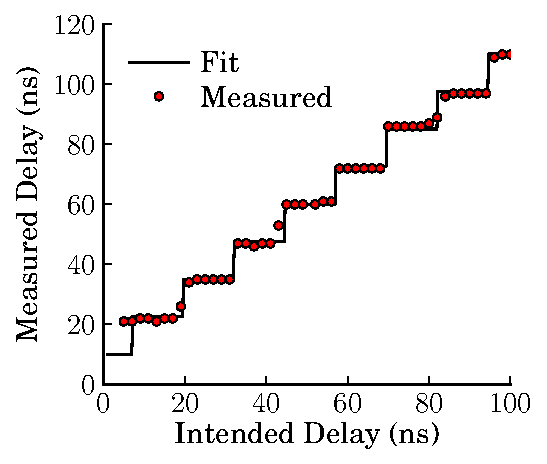
\includegraphics[width=.50\linewidth]{OLTP_eval/Delay.pdf}
  \caption{\textbf{Delay precision.} Delays are implemented by repeatedly reading the TSC register.  Resulting delays form a step function.  Inserted delays are within 6ns of the intended delay.}
  \label{fig::Delay}
\end{figure}

Figure~\ref{fig::Delay} shows the measured delay that results from iterating on an intended delay (both in ns).
Points show the median of ten thousand delay trials (a small number of trials result in excessively large delays and skew the mean).
The delay function resembles a step function---delays may only be inserted in multiples of the loop iteration latency.

To better understand delay behavior I perform a least squares regression of a step function against the measured data of the form:
$$delay(intended) = a \times floor(intended / a + b) + c$$
which results in an $R^2$ of .997 and the following parameter values: $a = 12.5$, $b=.434$, and $c=10.1$.
This indicates that each iteration takes 12.5ns.

As delays can only be introduced in steps I subtract 9.3ns from the intended delay to match to the closest step.
The resulting delay is within 6.25ns of the intended delay.
However, a given delay contains a constant skew (for example, an intended delay of 30ns always results in a 35ns delay).
As NVRAM persist latencies are expected to be in the hundreds of ns or greater, such error will negligibly affect my results.

\textbf{Modeling NVRAM persist bandwidth.}
In addition to NVRAM latency, I model shared NVRAM write bandwidth.
Using RDTSCP as a clock source, I maintain a shared \emph{next\_available} variable, representing the next clock tick in which the NVRAM device is available to be written.
Each NVRAM persist advances \emph{next\_available} to account for the latency of its persist operation.
Reservations take the maximum of \emph{next\_available} and the current RDTSCP and add the reservation duration.
The new value is atomically swapped into \emph{next\_available} via a Compare-And-Swap (CAS).
If the CAS fails (due to a race with a persist operation on another thread), the process repeats until it succeeds.
Upon success, the thread delays until the end of its reservation.
The main limitation of this approach is that it cannot model reservations shorter than the delay required to perform a CAS to a contended shared variable.
The delay incurred by a CAS instruction depends on contention to the address and the scheduling of threads across cores and processors.
I demonstrate that this technique models reservations above 120ns accurately, which is sufficient for my experiments.

Several factors affect the speed of bandwidth reservations (and therefore reservation accuracy) including the number of threads and their placement across sockets and cores.
I test the reservation system's accuracy by constraining thread placement while threads repeatedly reserve time and delay until the end of the reservation.
If all available time is reserved, reservation overhead is negligible and the modeled bandwidth is accurate.
However, when reservation length is sufficiently short reservation overheads will dominate, resulting in unreserved time.

\begin{table*}
  \centering
  \subtable[6 threads]{
    \label{table::Reservation::6}
    \begin{tabular}{l l l}
      \hline
      socket policy & spread cores & pack cores \\
      \hline \hline
      spread & 109 & 122 \\
      pack & 44 & 104 \\
      \hline
      \\
    \end{tabular}
  }
  \subtable[12 threads]{
    \label{table::Reservation::12}
    \begin{tabular}{l l l}
      \hline
      socket policy & spread cores & pack cores \\
      \hline \hline
      spread & 96 & 101 \\
      pack & 51 & 51 \\
      \hline
      \\
    \end{tabular}
  }
  \caption{\textbf{Bandwidth reservation bendmark.} Benchmark repeatedly reserves bandwidth as time and delays until end of the reservation.  Reservations are inaccurate if entire time cannot be reserved (reservation overhead dominates).  Results shown are reservation sizes (in ns) to reserve 99\% time.  We vary thread placement across CPU sockets and cores: packed (fill socket/core before allocating new) or spread (round robin assign to resources).  122ns and greater reservations accurately model constrained bandwidth.}
  \label{table::Reservation}
\end{table*}


Table~\ref{table::Reservation} shows the required reservation length (in ns) to reserve 99\% of time with six and 12 threads.
Additionally, the Table shows different thread placement across sockets and cores.
``Spread" implies assigning threads round-robin to resources, while ``pack" indicates that each resource is filled before assigning any threads to the next.
For example, assigning six threads in a pack sockets--spread cores policy (on a two socket server, each with six cores and two-way SMT) results in all six threads scheduled on the same socket but each thread on its own core (thus SMT is unused).
Such a configuration requires reservations of only 44ns to reserve 99\% of bandwidth-time.

Spreading threads across sockets or packing within cores slows reservations by requiring long-latency communication between sockets or forcing threads to contend with each other while scheduling instructions on cores.
At worst, when threads are spread across sockets and packed within cores a reservation length of 122ns is required to reserve 99\% of time.

A similar trend is true when considering 12 threads.
Packing threads into a socket completely fills all cores and SMT contexts of the socket (the bottom two cells represent the same configuration), needing 51ns reservations for accurate bandwidth modeling.
Spreading threads across sockets while packing cores requires 101ns to reserve 99\% of time.
The required time decreases from six to 12 threads as more threads are available to reserve time and it is less likely that time will go unreserved.

These results suggest that bandwidth reservations will be accurate, regardless of how threads are scheduled across processors and cores, so long as each reservation exceeds 120ns.
My additions to Shore-MT reserve bandwidth for each cache line persisted.
The persist bandwidth analysis study (presented later in Section~\ref{sec:OLTP_eval:Persists:Limitations}) shows that 35ns per cache line (approximately 1.7GB/s persists) represents sufficient bandwidth to negligibly limit performance.
Since at least four cache lines are always reserved together (in \texttt{persist\_page} and \texttt{persist\_wal}) the bandwidth reservation is accurate.

\textbf{NVRAM performance.}
I introduce NVRAM read and write delays separately.
Accurately modeling per-access increases in read latency is challenging, as reads are frequent and the expected latency increases on NVRAM compared to DRAM are small.
It is infeasible to use software instrumentation to model such latency increases at the granularity of individual reads; hardware support, substantial time dilation, or alternative evaluation techniques (e.g., simulation) would be required, all of which compromise accuracy and the ability to run experiments at full scale.
Instead, I use offline analysis with PIN \cite{LukCohn05} to determine (1) the reuse statistics of buffer cache pages, and (2) the average number of cache lines accessed each time a page is latched.
Together, these offline statistics provide an average number of cache line accesses per page latch event in Shore-MT.
I then introduce a delay at each latch based on the measured average number of misses and an assumed per-read latency increase based on the NVRAM technology.

I model NVRAM persist delays by annotating Shore-MT to track buffer cache writes at cache line granularity---64 bytes---using efficient ``dirty" bitmaps.
Depending on the recovery mechanism, I introduce delays corresponding to persist barriers and to model NVRAM write bandwidth contention.
Tracking buffer cache writes introduces less than a 3\% overhead to the highest throughput experiments.

I choose on-line timing modeling via software instrumentation in lieu of architectural simulations to allow experiments to execute at full scale and in real time.
While modeling aspects of NVRAM systems such as cache performance and more precise persist barrier delays require detailed hardware simulation, I believe NVRAM device and memory system design are not sufficiently established to consider this level of detail.
Instead, I investigate more general trends to determine if and when NVRAM read and write performance warrant storage management redesign.

\textbf{Recovery performance.} Figure~\ref{fig::Recovery} displays recovery latency vs transaction throughput for the TPCB workload, varying page flush rate.
Page flush rate is controlled by maintaining a constant number of dirty pages in the buffer cache, always flushing the page with the oldest volatile update.
Experiments run TPCB for one minute (sufficient to reach steady state behavior) and then kill the Shore-MT process.
Before starting recovery I drop the file system cache.
Reported recovery time includes only the recovery portion of the Shore-MT process; I do not include system startup time nor non-recovery Shore-MT startup time.

\textbf{Workloads.}
I use three workloads and transactions in this evaluation: TPCC, TPCB, and TATP.
TPCC models order management for a company providing a product or service \cite{TPCC}.
TPCB contains one transaction class and models a bank executing transactions across branches, tellers, customers, and accounts \cite{TPCB}.
TATP includes seven transactions to model a Home Location Registry used by mobile carriers \cite{TATP}.
Table~\ref{table::Workloads} shows the workload configuration.
%I choose a single updating transaction from each workload and size workloads to fit in a 12GB buffer cache.
I scale workloads to fit in a 12GB buffer cache.
Persist performance experiments use a single write-heavy transaction from each workload while read performance experiments use each workload's full mix.
All experiments report throughput as thousands of Transactions Per Second (kTPS).
Experiments perform ``power runs"---each thread generates and executes transactions continuously without think time---and run an optimal number of threads per configuration (between 10 and 12).

\begin{table}
  \centering
  \begin{tabular}{l l l l}
    \hline
    Workload & Scale factor & Size & Write transaction \\
    \hline \hline
    TPCC & 70 & 9GB & New order \\
    TPCB & 1000 & 11GB & \\
    TATP & 600 & 10GB & Update location \\
    \hline
  \end{tabular}
  \caption{\textbf{Workloads and transactions.}  One transaction class from each of three workloads, sized to approximately 10GB.}
  \label{table::Workloads}
\end{table}

\section{NVRAM Reads}
\label{sec:OLTP_eval:Reads}

I first evaluate database performance with respect to NVRAM reads.
Many candidate NVRAM technologies exhibit greater read latency than DRAM, possibly requiring additional hardware or software caching.
I wish to determine, for a given NVRAM read latency, how much caching is necessary to prevent slowdown, and whether it is feasible to provide this capacity in a hardware-controlled cache (otherwise software caches must be used).

\subsection{NVRAM Caching Performance}
\label{sec:OLTP_eval:Reads:Performance}

\textbf{Traces.}
\begin{table*}
  \centering
  \begin{tabulary}{\textwidth}{L L L L L L L L L}
    \hline
    & \multicolumn{2}{c}{TATP} & \multicolumn{2}{c}{TPCB} & \multicolumn{2}{c}{TPCC} & \multicolumn{2}{c}{Average} \\
    & \% lines & lines/latch & \% lines & lines/latch & \% lines & lines/latch & \% lines & lines/latch \\
    \hline \hline
    Store & 10.57\% & 5.32 & 11.71\% & 6.05 & 15.47\% &  4.25 & 12.58\% & 5.20 \\
    Index & 89.43\% & 11.27 & 82.41\% & 12.19 & 81.18\% & 11.17 & 84.34\% & 11.54 \\
    Other & 0.00\% & 0.00 & 5.89\% & 7.16 & 3.36\% & 3.00 & 3.08\% & 3.39 \\
    Total & & 5.53 & & 8.47 & & 6.14 & & 6.71 \\
    \hline
  \end{tabulary}
  \caption{\textbf{NVRAM access characteristics.} ``\% lines" indicates the percentage breakdown of cache line accesses.  ``lines/latch" reports the average number of cache line accesses per page latch.  Indices represent the majority of accesses.}
  \label{table::AccessCharacteristics}
\end{table*}

The NVRAM read-performance model combines memory access trace analysis with the timing model to measure transaction throughput directly in Shore-MT.
Traces consist of memory accesses to the buffer cache, collected running Shore-MT with PIN for a single transaction thread for two minutes.
I assume concurrent threads exhibit similar access patterns.
In addition, I record all latch events (acquire and release) and latch page information (i.e., table id, store type---index, heap, or other).
I analyze traces at cache line (64 bytes) and page (8KB) granularity.

These traces provide insight into how Shore-MT accesses persistent data, summarized in Table~\ref{table::AccessCharacteristics}.
Index accesses represent the great majority of cache line accesses, averaging 85\% of accesses to NVRAM across workloads.
Any caching efforts should focus primarily on index pages and cache lines.
Note also that indexes access a greater number of cache lines per page access than other page types (average 11.48 vs 4.85 for heap pages and 4.77 for other page types), suggesting that uncached index page accesses have the potential to introduce greater delays.

\textbf{Throughput.}
\begin{figure}
  \centering
  \subfigure[TATP]{\label{fig::ReadPerformance::TATP} 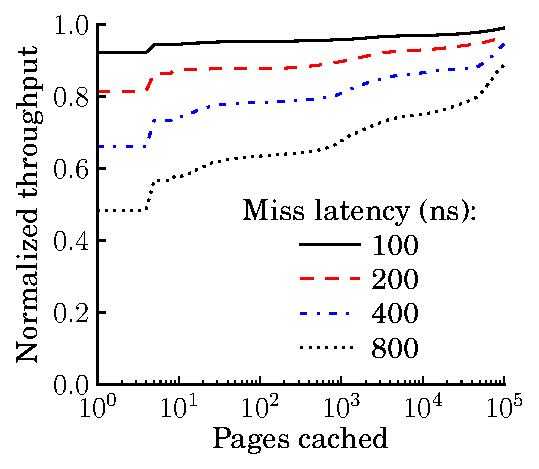
\includegraphics[width=.49\textwidth]{OLTP_eval/ReadPerformance_TATP.pdf}}
  \subfigure[TPCB]{\label{fig::ReadPerformance::TPCB}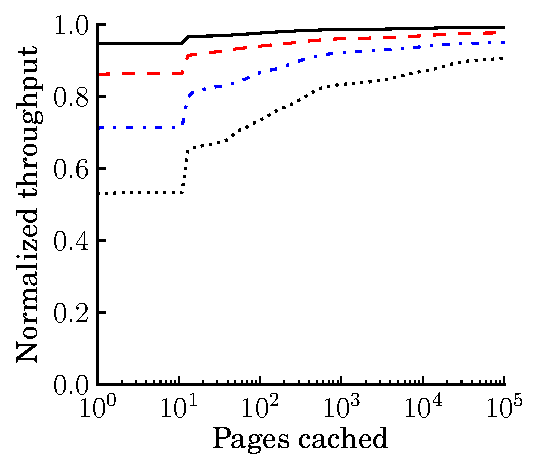
\includegraphics[width=.49\textwidth]{OLTP_eval/ReadPerformance_TPCB.pdf}}
  \subfigure[TPCC]{\label{fig::ReadPerformance::TPCC}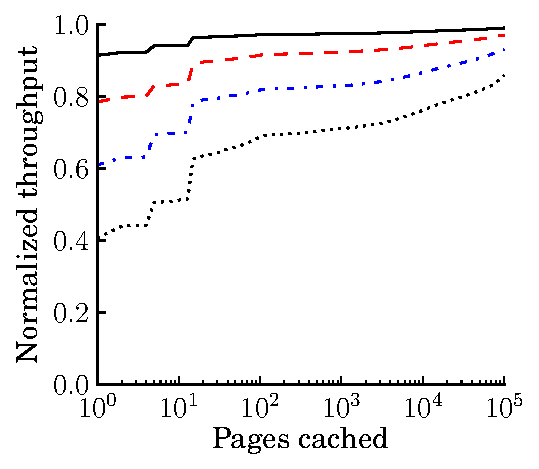
\includegraphics[width=.49\textwidth]{OLTP_eval/ReadPerformance_TPCC.pdf}}
%  \begin{subfigure}{0.32\textwidth}
%    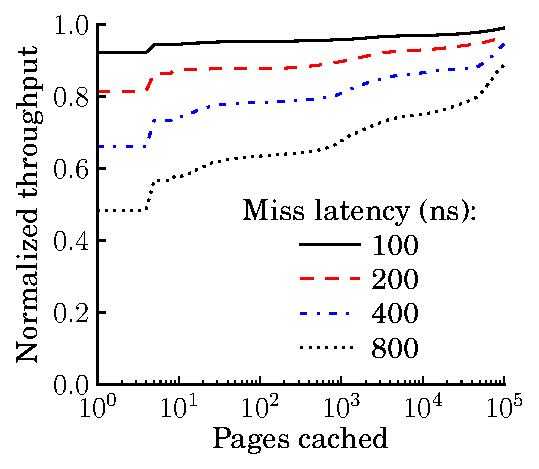
\includegraphics[width=\textwidth]{OLTP_eval/ReadPerformance_TATP.pdf}
%    \caption{TATP}
%    \label{fig::ReadPerformance::TATP}
%  \end{subfigure}
%  \begin{subfigure}{0.32\textwidth}
%    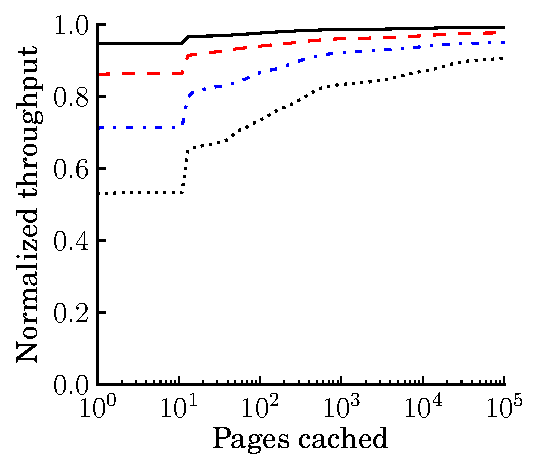
\includegraphics[width=\textwidth]{OLTP_eval/ReadPerformance_TPCB.pdf}
%    \caption{TPCB}
%    \label{fig::ReadPerformance::TPCB}
%  \end{subfigure}
%  \begin{subfigure}{0.32\textwidth}
%    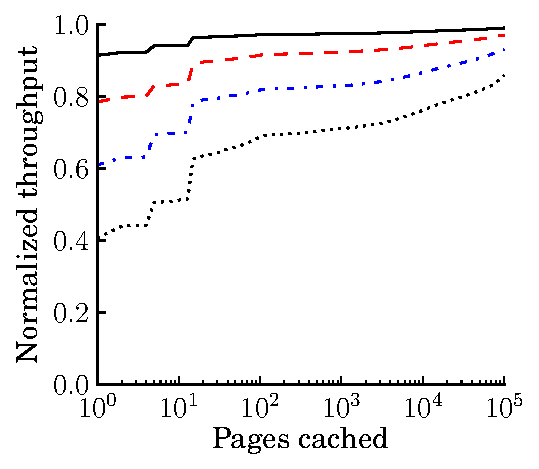
\includegraphics[width=\textwidth]{OLTP_eval/ReadPerformance_TPCC.pdf}
%    \caption{TPCC}
%    \label{fig::ReadPerformance::TPCC}
%  \end{subfigure}
  \caption{\textbf{Throughput vs NVRAM read latency.} 100ns miss latency suffers up to a 10\% slowdown over DRAM.  Higher miss latencies introduce large slowdowns, requiring caching.  Fortunately, even small caches effectively accelerate reads.}
  \label{fig::ReadPerformance}
\end{figure}

I create a timing model in Shore-MT from the previous memory traces.
Given traces, I perform cache analysis at page granularity, treating latches as page accesses and assuming a fully associative cache with a least-recently-used replacement policy (LRU).
Cache analysis produces an average page miss rate to each table.
I conservatively assume that every cache line access within an uncached page introduces an NVRAM stall, neglecting optimizations such as out-of-order execution and simultaneous multi-threading that might hide some NVRAM access stalls. 
The model assumes the test platform incurs a 50ns DRAM fetch latency, and adds additional latency to mimic NVRAM (for example, a 200ns NVRAM access adds 150ns delay per cache line).
I combine average page miss rate and average miss penalty (from lines/latch in table~\ref{table::AccessCharacteristics}) to compute the average delay incurred per latch event.
This delay is inserted at each page latch acquire in Shore-MT, using \InPlace, to produce a corresponding throughput.

Figure~\ref{fig::ReadPerformance} shows throughput achieved for the three workloads while varying the number of pages cached (horizontal axis) and NVRAM miss latency (various lines).
The vertical axis displays throughput normalized to DRAM-miss-latency's throughput (no additional delay inserted).
Without caching, throughput suffers as NVRAM miss latency increases, shown at the extreme left of each graph.
A 100ns miss latency consistently achieves at least 90\% of potential throughput.
However, an 800ns miss latency averages only 50\% of the potential throughput, clearly requiring caching.
TPCB and TPCC see a 10-20\% throughput improvement for a cache size of just 20 pages.
As cache capacity further increases, each workload's throughput improves to varying degrees.
A cache capacity of 100,000 (or 819MB at 8KB pages) allows NVRAMs with 800ns miss latencies to achieve at least 80\% of the potential throughput.
While too large for on-chip caches, such a buffer might be possible as a hardware-managed DRAM cache \cite{QureshiSrinivasan09}.

\subsection{Analysis}
\label{sec:OLTP_eval:Reads:Analysis}
\begin{figure}
  \centering
  \subfigure[TATP]{\label{fig::Caching::TATP} 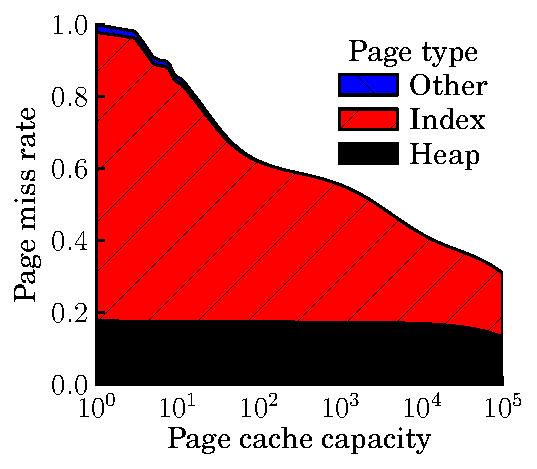
\includegraphics[width=.45\textwidth]{OLTP_eval/Caching_TATP.pdf}}
  \subfigure[TPCB]{\label{fig::Caching::TPCB}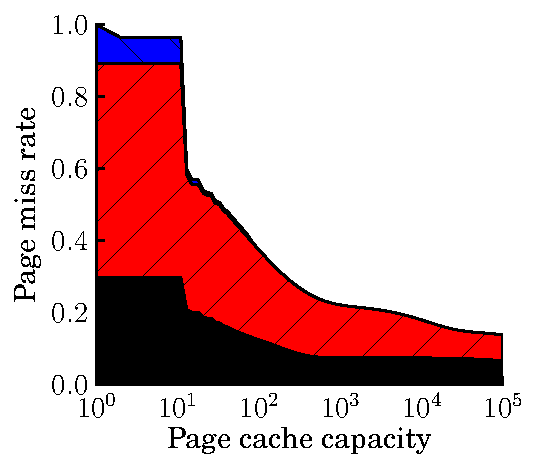
\includegraphics[width=.45\textwidth]{OLTP_eval/Caching_TPCB.pdf}}
  \subfigure[TPCC]{\label{fig::Caching::TPCC}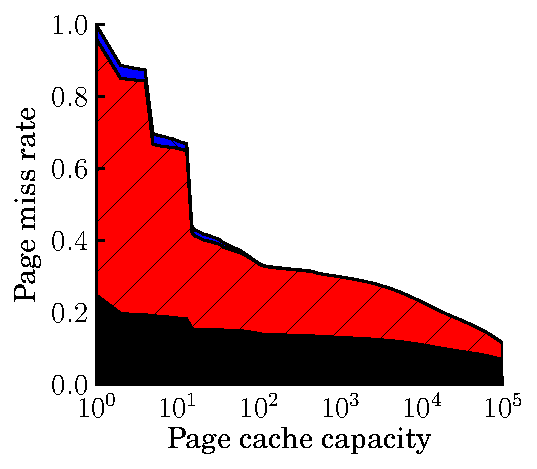
\includegraphics[width=.45\textwidth]{OLTP_eval/Caching_TPCC.pdf}}
  \caption{\textbf{Page caching effectiveness.} High level B+Tree pages and append-heavy store pages cache effectively.  Other pages cache as capacity approaches table size.}
  \label{fig::Caching}
\end{figure}

I have shown that modest cache sizes effectively hide NVRAM read stalls for these workloads, and further analyze caching behavior to reason about OLTP performance more generally.
Figure~\ref{fig::Caching} shows the page miss rate per page type (index, heap, or other) as page cache capacity increases.
Each graph begins at one at the left---all page accesses miss for a single-page cache.
As cache capacity increases, workloads see their miss rates start to decrease between cache capacity of five and 20 pages.
TATP experiences a decrease in misses primarily in index pages, whereas TPCB and TPCC see decreases across all page types.

While cache behavior is specific to each workload, the results represent trends applicable to many databases and workloads, specifically, index accesses and append-heavy tables.
First, all workloads see a decrease in index page misses as soon as B+Tree roots (accessed on every traversal) successfully cache.
The hierarchical nature of B+Tree indexes allows high levels of the tree to cache effectively for even a small cache capacity.
Additionally, TPCB and TPCC contain history tables to which data are primarily appended.
Transactions append to the same page as previous transactions, allowing such tables to cache effectively.
Similarly, extent map pages used for allocating new pages and locating pages to append into are frequently accessed and likely to cache.
The remaining tables' pages are accessed randomly and only cache as capacity approaches the size of each table.
In the case of TPCB and TPCC, each transaction touches a random tuple of successively larger tables (Branch, Teller, and Account for TPCB; Warehouse, District, Customer, etc. for TPCC).
This analysis suggests that various page types, notably index and append-heavy pages, cache effectively, accelerating throughput for high-latency NVRAM misses with small cache capacities.

\textbf{Main-memory databases.}
While I use Shore-MT (a disk-based storage manager) as a research platform, main-memory database optimizations (e.g., \cite{DiaconuFreedman13, BallardBehman11, Oracle09}) also apply to byte-addressable NVRAM.
Main-memory databas\-es assume heap data resides solely in byte-addressable memory, improving throughput relative to traditional disk-back\-ed storage by removing expensive indirection (i.e., using memory pointers instead of buffer translation tables), reducing overheads associated with concurrency control and latches, and optimizing data layout for caches and main-memory, among other optimizations.
While such optimizations will increase transaction throughput, removing non-NVRAM overheads will amplify the importance of read-miss latency (an equal increase in NVRAM read-miss latency will yield a relatively greater drop in performance).
At the same time, data layout optimizations will reduce the number of cache lines and memory rows accessed per action (e.g., per latch), minimizing NVRAM read overheads.
Investigating main-memory database optimizations for NVRAM remains future work.

\begin{table}
  \centering
  \begin{tabular}{l l}
    \hline
    Workload & Bandwidth (GB/s) \\
    \hline \hline
    TATP & 0.977 \\
    TPCB & 1.044 \\
    TPCC & 1.168 \\
    \hline
  \end{tabular}
  \caption{\textbf{Required NVRAM read bandwidth.} Workloads require up to 1.2 GB/s read bandwith.}
  \label{table::ReadBandwidth}
\end{table}

\textbf{Bandwidth.}
Finally, I briefly address NVRAM read bandwidth.
For a worst-case analysis, I assume no caching.
Given the average number of cache line accesses per page latch, the average number of page latches per transaction, and transaction throughput (taken from Section~\ref{sec:OLTP_eval:Persists}), I compute worst-case NVRAM read bandwidth for each workload, shown in Table~\ref{table::ReadBandwidth}.
The considered workloads require at most 1.2 GB/s (TPCC).
Since this is within expected NVRAM bandwidth constraints and caching reduces the required bandwidth further, I conclude that NVRAM read bandwidth for persistent data on OLTP is not a performance concern.

\subsection{Summary}
\label{sec:OLTP_eval:Reads:Summary}
NVRAM presents a new storage technology, requiring new optimizations for database systems.
Increased memory read latencies require new consideration for database caching systems.
I show that persistent data for OLTP can be cached effectively, even with limited cache capacity.
I expect future NVRAM software to leverage hardware caches, omitting software buffer caches.
Next, I turn to write performance for storage management on NVRAM devices.

\section{NVRAM Persist Synchronization}
\label{sec:OLTP_eval:Persists}

Whereas NVRAM reads benefit from caching, persists must always access the storage device.
Of particular insterest is the cost of ordering persists via persist barriers.
Several factors increase persist barrier latency, including ordering persists across distributed/NUMA memory architectures, long latency interconnects (e.g., PCIe-attached storage), and slow NVRAM MLC cell persists.
I consider the effect of persist barrier latency on transaction processing throughput to determine if and when new NVRAM technologies warrant redesigning recovery management.

Refer to Sections~\ref{sec:OLTP_design:Design} and~\ref{sec:OLTP_design:Methodology} for a more thorough description of recovery mechanisms and experimental setup.
All experiments throttle persist bandwidth to 1.5GB/s, which I believe to be conservative (already possible with PCIe-attached Flash).
Ideally, NVRAM will provide low latency access, enabling \InPlace.
However, one would expect \InPlace's performance to suffer at large persist barrier latencies, requiring either \NVDisk or \GroupCommit to regain throughput.

\subsection{Persist Barrier Latency}
\label{sec:OLTP_eval:Persists:Performance}

\begin{figure*}
  \centering
  %\begin{subfigure}{0.32\textwidth}
  %  \includegraphics[width=\textwidth]{figures/pdfs/PersistLatencyThroughput/TATP.pdf}
  %  \caption{TATP}
  %  \label{fig::PersistLatencyThroughput::TATP}
  %\end{subfigure}
  %\begin{subfigure}{0.32\textwidth}
  %  \includegraphics[width=\textwidth]{figures/pdfs/PersistLatencyThroughput/TPCB.pdf}
  %  \caption{TPCB}
  %  \label{fig::PersistLatencyThroughput::TPCB}
  %\end{subfigure}
  %\begin{subfigure}{0.32\textwidth}
  %  \includegraphics[width=\textwidth]{figures/pdfs/PersistLatencyThroughput/TPCC.pdf}
  %  \caption{TPCC}
  %  \label{fig::PersistLatencyThroughput::TPCC}
  %\end{subfigure}
  \subfigure[TATP]{\label{fig::PersistLatencyThroughput::TATP} 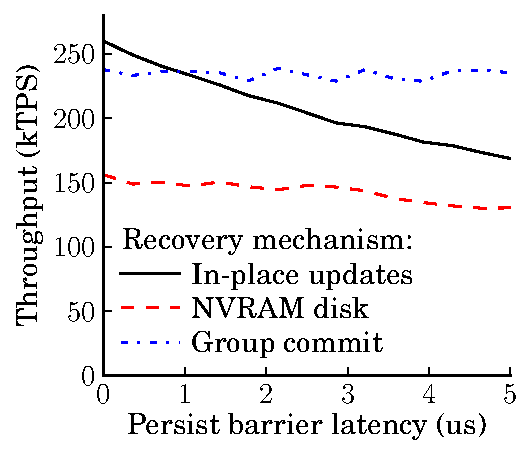
\includegraphics[width=.45\textwidth]{OLTP_eval/PersistLatencyThroughput_TATP.pdf}}
  \subfigure[TPCB]{\label{fig::PersistLatencyThroughput::TPCB}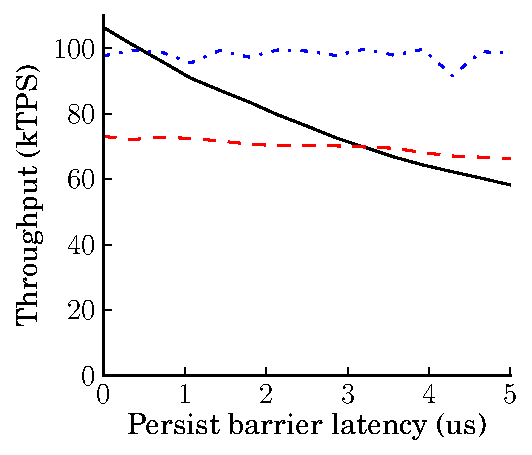
\includegraphics[width=.45\textwidth]{OLTP_eval/PersistLatencyThroughput_TPCB.pdf}}
  \subfigure[TPCC]{\label{fig::PersistLatencyThroughput::TPCC}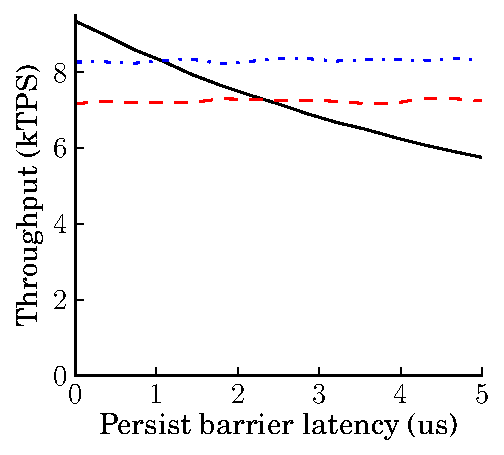
\includegraphics[width=.45\textwidth]{OLTP_eval/PersistLatencyThroughput_TPCC.pdf}}
  \caption{\textbf{Throughput vs persist barrier latency.} \InPlace performs best for zero-cost persist barriers, but throughput suffers as persist barrier latency increases.  \NVDisk and \GroupCommit are both insensitive to increasing persist barrier latency, with \GroupCommit offering higher throughput.}
  \label{fig::PersistLatencyThroughput}
\end{figure*}


Figure~\ref{fig::PersistLatencyThroughput} shows throughput for write-heavy transactions as persist barrier latency increases from 0\textmu s to 5\textmu s, the range believed to encompass realistic latencies for possible implementations of persist barriers and storage architectures.
A persist barrier latency of 0\textmu s (left edge) corresponds to no barrier/DRAM latency.
For such devices (e.g., battery-backed DRAM), \InPlace far out-paces \NVDisk, providing up to a 50\% throughput improvement.
The speedup stems from a combination of removing WAL overheads, removing contention between page flushers and transaction threads, and freeing up (a few) threads from log and page flushers to run additional transactions.
\InPlace also outperforms \GroupCommit, providing an average 10\% throughput improvement across workloads.

As persist barrier latency increases, each recovery mechanism reacts differently.
\InPlace, as expected, loses throughput.
\NVDisk and \GroupCommit, on the other hand, are both insensitive to persist barrier latency; their throughputs see only a small decrease as persist barrier latency increases.
TATP sees the largest throughput decrease for \NVDisk (14\% from 0\textmu s to 5\textmu s).
The decrease stems from \NVDisk's synchronous commits, requiring the log flusher thread to complete flushing before transactions commit.
During this time, transaction threads sit idle.
While both \NVDisk and \GroupCommit retain high throughput, there is a large gap between the two, with \GroupCommit providing up to a 50\% performance improvement over \NVDisk.
This difference, however, is workload dependent, with WAL imposing a greater bottleneck to TATP than to TPCB or TPCC.

Of particular interest are persist barrier latencies where lines intersect---the break-even points for determining the optimal recovery mechanism.
Whereas all workloads prefer \InPlace for a 0\textmu s persist barrier latency, \GroupCommit provides better throughput above 1\textmu s persist barrier latency.
When only considering \InPlace and \NVDisk the decision is less clear.
Over the range of persist barrier latencies TATP always prefers \InPlace to \NVDisk (the break-even latency is well above 5\textmu s).
TPCB and TPCC see the two mechanisms intersect near 3.5\textmu s and 2.5\textmu s, respectively, above which \NVDisk provides higher throughput.
TATP, unlike the other two workloads, only updates a single page per transaction.
Other overheads tend to dominate transaction time, resulting in a relatively shallow \InPlace curve.

\begin{table}
  \centering
  \begin{tabular}{l l l}
    \hline
    Workload & Full mix & Single transaction \\
    \hline \hline
    TATP & 25 & 12 \\
    TPCB & 3.2 & 3.2 \\
    TPCC & 3.6 & 2.4 \\
    \hline
  \end{tabular}
  \caption{\textbf{Break-even persist latency} Persist barrier latency (\textmu s) where \NVDisk and \InPlace achieve equal throughput.  Latencies reported for full transaction mixes and single write-heavy transaction per workload.}
  \label{table::PersistLatencyBreakeven}
\end{table}


The previous results show throughput only for a single transaction from each workload.
Table~\ref{table::PersistLatencyBreakeven} shows break-even persist barrier latency between \NVDisk and \InPlace for these transactions and full transaction mixes.
Full transaction mixes contain read-only transactions, reducing log insert and persist barrier frequency (read-only transactions require no recovery).
\NVDisk sees improved throughput at 0 \textmu s and \InPlace's throughput degrades less quickly as persist barrier latency increases.
As a result, the break-even persist barrier latency between these two designs increases for the full transaction mix relative to a single write-heavy transaction and the opportunity to improve throughput by optimizing recovery management diminishes---improved recovery management does not affect read-only transactions and actions.

These results suggest different conclusions across storage architectures.
NVRAM connected via the main memory bus will provide low latency persist barriers (less than 1\textmu s) and prefer \InPlace.
Other storage architectures, such as distributed storage, require greater delays to synchronize persists.
For such devices, \GroupCommit offers an alternative to \NVDisk that removes software overheads inherent in WAL while providing recovery.
However, \GroupCommit increases transaction latency.

\subsection{Transaction Latency}
\label{sec:OLTP_eval:Persists:XctLatency}

\begin{figure*}
  \centering
  %\begin{subfigure}{0.32\textwidth}
  %  \includegraphics[width=\textwidth]{figures/pdfs/XctLatency/TATP.pdf}
  %  \caption{TATP}
  %  \label{fig::XctLatency::TATP}
  %\end{subfigure}
  %\begin{subfigure}{0.32\textwidth}
  %  \includegraphics[width=\textwidth]{figures/pdfs/XctLatency/TPCB.pdf}
  %  \caption{TPCB}
  %  \label{fig::XctLatency::TPCB}
  %\end{subfigure}
  %\begin{subfigure}{0.32\textwidth}
  %  \includegraphics[width=\textwidth]{figures/pdfs/XctLatency/TPCC.pdf}
  %  \caption{TPCC}
  %  \label{fig::XctLatency::TPCC}
  %\end{subfigure}
  \subfigure[TATP -- Update Location]{\label{fig::XctLatency::TATP} 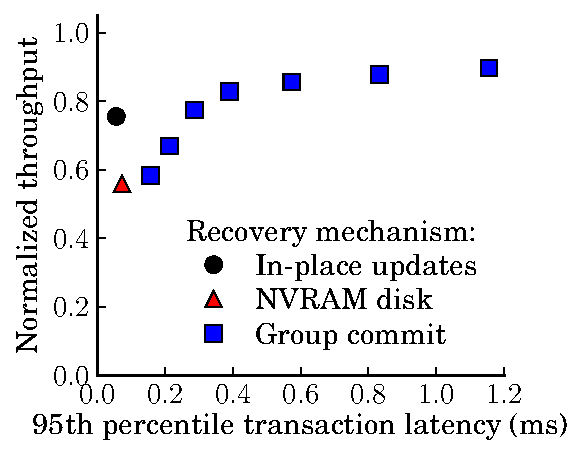
\includegraphics[width=.45\textwidth]{OLTP_eval/XctLatency_TATP.pdf}}
  \subfigure[TPCB]{\label{fig::XctLatency::TPCB}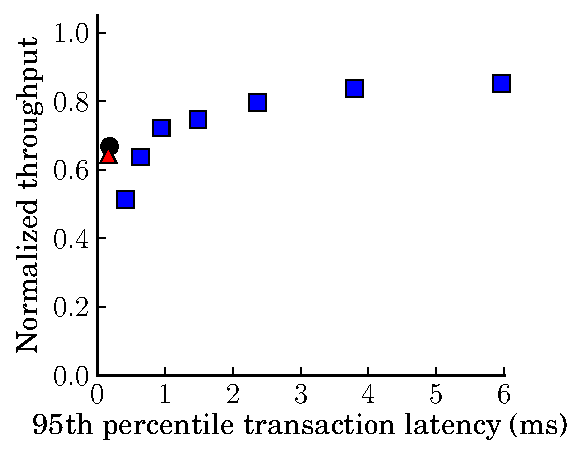
\includegraphics[width=.45\textwidth]{OLTP_eval/XctLatency_TPCB.pdf}}
  \subfigure[TPCC -- New Order]{\label{fig::XctLatency::TPCC}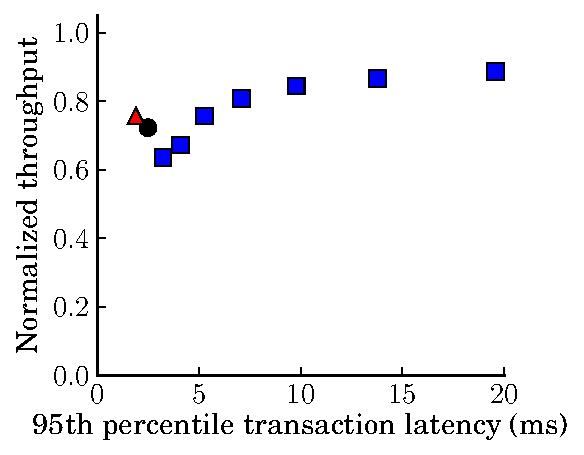
\includegraphics[width=.45\textwidth]{OLTP_eval/XctLatency_TPCC.pdf}}
  \caption{\textbf{95th percentile transaction latency.} All graphs are normalized to 0\textmu s persist barrier latency \InPlace throughput.  Experiments use 3\textmu s persist barrier latency.  \GroupCommit avoids high latency persist barriers by defering transaction commit, committing entire batches atomically.}
  \label{fig::XctLatency}
\end{figure*}


\GroupCommit improves transaction throughput by placing transactions into batches and committing all transactions in a batch atomically.
Doing so minimizes and limits the number of persist barriers.
However, deferring transaction commit increases transaction latency, especially for the earliest transactions in each batch.
To achieve reasonable throughput, batches must be significantly longer than average transaction latency (such that batch execution time dominates batch quiesce and persist time).
The batch period acts as a knob for database administrators to trade off transaction latency and throughput.
I use this knob to measure the relationship between throughput and high-percentile transaction latency.

Figure~\ref{fig::XctLatency} shows throughput, normalized to \InPlace at 0\textmu s persist barrier latency.
The results consider a 3\textmu s persist barrier latency, where \GroupCommit provides a throughput improvement over other recovery mechanisms.
The different \GroupCommit points represent different batch periods, and I report the measured 95th percentile transaction latency for all recovery mechanisms.
I measure transaction latency from the time a transaction begins to the time its batch ends (Shore-MT does not model any pre-transaction queuing time).

The results illustrate that \GroupCommit is capable of providing equivalent throughput to the other recovery mechanisms with reasonable latency increases (no more than 5\texttimes).
Further, high-percentile transaction latencies fall well below the latency expectations of modern applications.
TPCC, the highest latency workload, approaches optimal throughput with a 95th percentile transaction latency of 15ms---similar to latencies incurred by disk-backed databases.
For latency sensitive workloads, the batch period can be selected to precisely control latency, and \InPlace and \NVDisk remain alternatives.

\subsection{NVRAM Persist Limitations}
\label{sec:OLTP_eval:Persists:Limitations}

In addition to persist delays NVRAM may suffer limitations due to persist bandwidth and write endurance.
I quantify these limitations and determine how database design affects each.

\textbf{Persist bandwidth.}
Different NVRAM storage architectures impose a variety of limitations on persist bandwidth (e.g., memory bus-attached NVRAM will allow greater throughput than PCIe-attached NVRAM).
Different software designs place varying requirements on bandwidth.

\begin{figure}
  \centering
  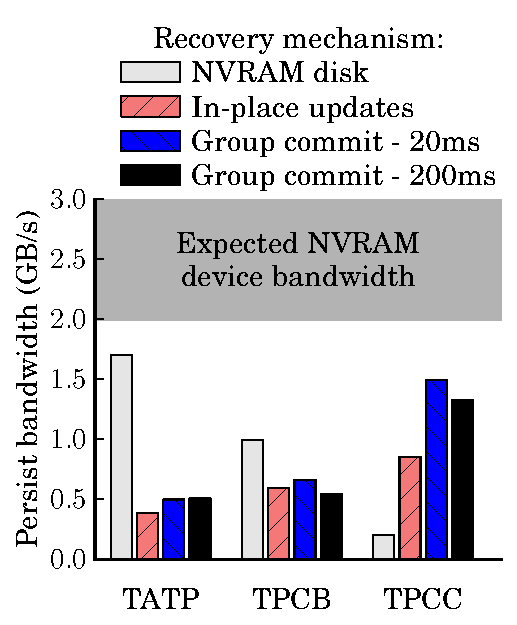
\includegraphics[width=.9\linewidth]{OLTP_eval/Bandwidth.pdf}
  \caption{\textbf{Required NVRAM bandwidth.} Persist/write bandwidth required to achieve 95\% performance relative to no bandwidth constraint.  Bandwidth requirements are far below expected device bandwidth.}
  \label{fig::Bandwidth}
\end{figure}

Figure~\ref{fig::Bandwidth} shows the bandwidth required for each workload and recovery mechanism to achieve 95\% throughput compared to same configuration with no bandwidth constraint.
Each recovery mechanism sees different bandwidth requirements, and required bandwidth varies across workloads.

The \NVDisk configuration flushes pages aggressively (attempts to flush continuously) and consumes all available bandwidth.
Since bandwidth is restricted recovery latency may increase (not reflected in the results).
Page flushing contends with log flushing for bandwidth, but so long as log flushes are minimally delayed throughput will not be affected.
TATP, which contains short transactions, requires the most bandwidth (1.7GB/s) to reduce transaction commit delays.
I believe that asynchronous commit (allowing a new transaction to begin processing on the hardware thread while the previous transaction waits to commit) would lower the bandwidth requirement.
TPCC, on the other hand, has long transactions and transaction commit is less of a concern.

\InPlace requires the least bandwidth of the recovery mechanisms.
TATP's Update Location transaction needs only 0.4GB/s since each transaction contains a single small update.
TPCC's New Order transaction modifies much more data, requiring 0.8GB/s persist bandwidth to achieve 95\% throughput.

Finally, \GroupCommit sees varying requirements on persist bandwidth.
All persists occur at batch boundaries, resulting in persist bursts.
I consider two batch periods---20ms and 200ms.
TATP and TPCC require relatively small bandwidths while TPCC requires over 1.5GB/s persist bandwidth to achieve 95\% throughput.
The bursty nature of \GroupCommit and large modifications by TPCC's New Order transaction result in persist bandwidth quickly creating a bottleneck.
Longer batches help slightly by allowing updates to coalesce within the batch, reducing the total number of bytes persisted.
The bandwidth requirements would be reduced by introducing mechanisms to enable early persists (persist data before the batch ends), removing persist bursts.

While persist bandwidth requirements vary, the strictest configuration (\NVDisk for TATP) requires only 1.7GB/s.
Such bandwidth is currently possible with existing PCIe Flash memory SSDs, and I believe is attainable for all candidate NVRAM technologies.
I expect that persist bandwidth will not be a concern for OLTP systems using NVRAM.

\textbf{Device lifetime.}
NVRAM technologies, much like Flash memory currently, will have limited write endurance; each cell may only be reliably written a finite number of times.
Device lifetime is generally determined by the most frequently written addresses.
Previous work proposes hardware techniques to evenly distribute writes amongst cells by constantly changing the mapping between between memory addresses and the underlying memory cell \cite{QureshiKaridis09}.
These techniques prolong device lifetime by ensuring that frequently written addresses do not wear out individual cells.
While the recovery mechanisms presented here each produce varying persist rates with different abilities to naturally distribute persists across addresses, it is unclear if software mechanisms are sufficient to prolong device lifetime.

\begin{figure*}
  \centering
  \subfigure[No wear leveling]{\label{fig::WearLeveling::None} 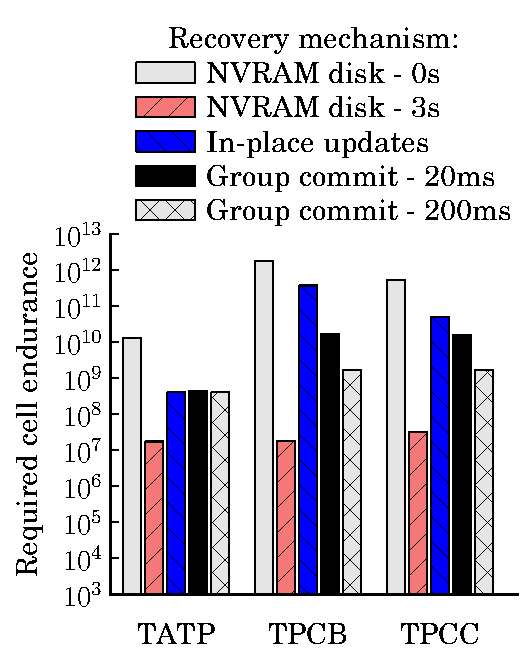
\includegraphics[width=.49\textwidth]{OLTP_eval/WearLeveling_None.pdf}}
  \subfigure[Perfect wear leveling]{\label{fig::WearLeveling::Perfect}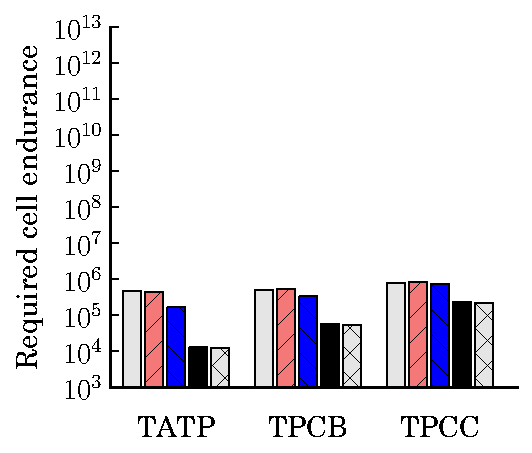
\includegraphics[width=.49\textwidth]{OLTP_eval/WearLeveling_Perfect.pdf}}
  \caption{\textbf{NVRAM cell endurance for 10-year lifetime.}  Without hardware wear leveling the most-written cell limits device lifetime.  \NVDisk requires conservative page flushing (3s recovery latency vs 0s, instantaneous, recovery) and \GroupCommit requires longer batch periods (200ms vs 20ms) to improve device lifetime.  We expect hardware wear leveling to always be required with \InPlace.  With perfect wear leveling (all writes occur evenly throughout cells in the device) and a 32GB storage device all workloads and configurations achieve a 10-year device lifetime for cell endurance of $10^6$ writes and greater.}
  \label{fig::WearLeveling}
\end{figure*}

Figure~\ref{fig::WearLeveling} shows the required cell endurance (number of persists) to achieve a 10-year device lifetime assuming the database runs at maximum throughput continuously.
All recovery mechanisms assume \InPlace's throughput for a more fair comparison.
Persists are tracked at byte granularity.
I consider two scenarios: no wear leveling---lifetime is limited by the most frequently written address---and perfect wear leveling---all persists are evenly distributed across all physical addresses (provided in hardware).
I consider \NVDisk with both instantaneous recovery and 3s recovery latency, \InPlace, and \GroupCommit with 20ms and 200ms batch latencies.
Logs are implemented as circular buffers.
Thus, logs do not contribute to the most written byte and have no bearing on device lifetime when hardware wear leveling is unavailable.
Perfect wear leveling assumes a 32GB device.

Without hardware wear leveling \NVDisk with instantaneous recovery (aggressive page flushing) and \InPlace require the greatest cell endurance.
Both mechanisms persist each update directly to the NVRAM store.
\NVDisk must additionally persist LSNs, which constitute the most frequently persisted addresses, while LSNs are no longer used with \InPlace and \GroupCommit.
Both of these configurations require greater cell endurance far greater than $10^8$ writes, the endurance expected of phase change memory \cite{BurrKurdi08}.

\NVDisk with 3s recovery latency requires much lower cell endurance for a 10 year lifetime.
Writes to heap pages coalesce and only occasionally persist to NVRAM.
\NVDisk effectively increases device lifetime by reducing the total number of persists and limiting the rate that any single page may write back.
However, doing so requires an increase in recovery latency.
\NVDisk may possibly provide acceptable software wear leveling so long as recovery latency is reasonable.

Finally, \GroupCommit provides wear leveling by only allowing a single persist to each address per batch (all other persists coalesce).
However, neither 20ms nor 200ms batches is capable of coalescing enough writes to guarantee a 10 year device lifetime.
\GroupCommit would require far too large a batch period, increasing transaction latency, to reliably wear-level NVRAM.

When hardware distributes persists evenly across NVRAM cells all recovery mechanisms achieve a 10 year lifetime assuming $10^8$ writes per cell.
In this case lifetime is determined by the total number of persists rather than the most-persisted address.
Due to the inability of software to reliably and sufficiently extend device lifetime, and the effectiveness of hardware wear leveling, I expect future NVRAM SSDs to include hardware wear leveling.

\subsection{Summary}
\label{sec:OLTP_eval:Persists:Summary}
Persist barriers used to enforce persist order pose a new performance obstacle to providing recoverable storage management with NVRAM.
I show that, for memory bus-attached NVRAM devices, ensuring recovery using \InPlace is a viable strategy that provides high throughput and removes the overheads of WAL.
For interconnects and NVRAM technologies that incur larger persist barrier delays, \GroupCommit offers an alternative that yields high throughput and reasonable transaction latency.
\GroupCommit's batch period allows precise control over transaction latency for latency-critical applications.
Finally, I demonstrate that persist bandwidth is not a concern, and that while \NVDisk may provide an effective mechanism to cope with limited write endurance I expect future devices to include hardware wear leveling.

%\section{Proposed Work}
%\label{sec:OLTP_eval:Proposed}
%
%I propose to include two additional studies.
%These studies were originally conducted for an earlier journal submission; the experimental system has changed substantially since then.
%
%\textbf{Persist bandwidth.}
%\begin{figure}
  \centering
  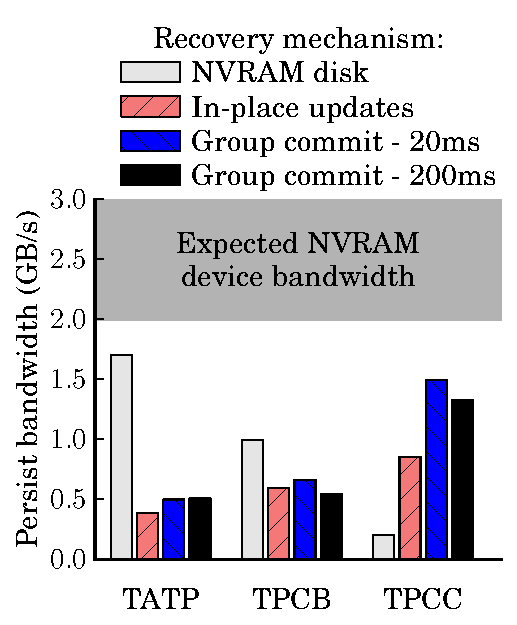
\includegraphics[width=.9\linewidth]{OLTP_eval/Bandwidth.pdf}
  \caption{\textbf{Required NVRAM bandwidth.} Persist/write bandwidth required to achieve 95\% performance relative to no bandwidth constraint.  Bandwidth requirements are far below expected device bandwidth.}
  \label{fig::Bandwidth}
\end{figure}

%Different NVRAM storage architectures impose a variety of limitations on persist bandwidth (e.g., memory bus-attached NVRAM will allow greater throughput than PCIe-attached NVRAM).
%I intend to study the persist bandwidth requirements for each recovery mechanism.
%
%Recovery mechanisms display interesting behaviors with respect to bandwidth.
%\NVDisk persists inefficiently with respect to the total number of bytes updated; even a small page update requires large log entries.
%However, the log persist makes effective use of cache lines (the granularity that data must transfer to the memory device).
%Further, when increased recovery latency is allowable, bandwidth usage may be decreased by deferring page flushing, allowing writes to coalesce in pages.
%The result is that \NVDisk makes reasonable use of bandwidth, and bandwidth constraints are unlikely to limit throughput.
%
%\InPlace displays similar bandwidth usage to \NVDisk.
%All page updates must persist to NVRAM, and these updates tend to use cache lines ineffectively (only a small portion of each cache line changes).
%Also similarly to \NVDisk, \InPlace must maintain ARIES logs (although per-transaction and undo-only), requiring large persists.
%
%\GroupCommit, while persisting the least amount of data, is the most sensitive to persist bandwidth constraints.
%The total quantity of data is reduced by using physical logs -- logs copy data with little associated metadata.
%Additionally, updates in each batch coalesce.
%Only the first write to a given address produces undo, and only the final write to that address persists in-place.
%Other versions of data during the batch do not persist.
%The downside of \GroupCommit is that persists occur in bursts between batches.
%No data persists while the batch executes.
%Between batches however, all logs and heap data persists, placing huge requirements on bandwidth.
%I intend to include a quantitative study of this behavior.
%
%\textbf{Device lifetime.}
%\begin{figure*}
  \centering
  \subfigure[No wear leveling]{\label{fig::WearLeveling::None} 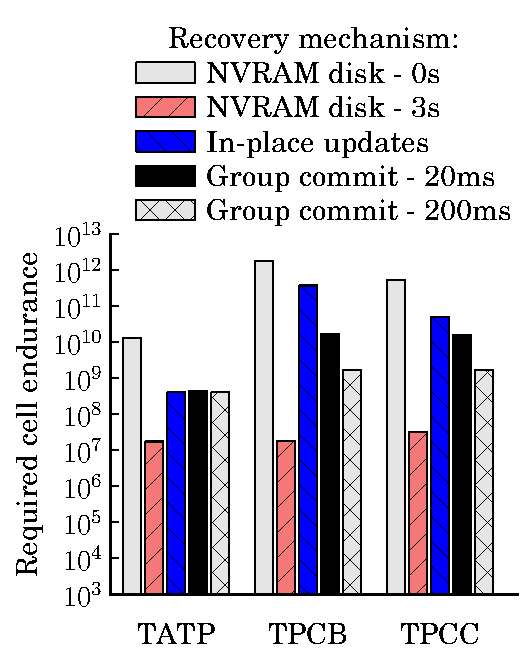
\includegraphics[width=.49\textwidth]{OLTP_eval/WearLeveling_None.pdf}}
  \subfigure[Perfect wear leveling]{\label{fig::WearLeveling::Perfect}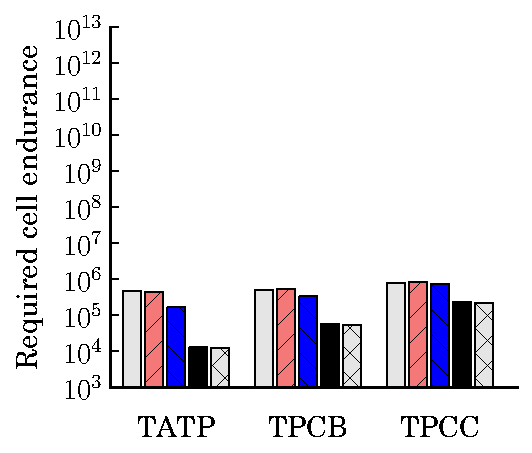
\includegraphics[width=.49\textwidth]{OLTP_eval/WearLeveling_Perfect.pdf}}
  \caption{\textbf{NVRAM cell endurance for 10-year lifetime.}  Without hardware wear leveling the most-written cell limits device lifetime.  \NVDisk requires conservative page flushing (3s recovery latency vs 0s, instantaneous, recovery) and \GroupCommit requires longer batch periods (200ms vs 20ms) to improve device lifetime.  We expect hardware wear leveling to always be required with \InPlace.  With perfect wear leveling (all writes occur evenly throughout cells in the device) and a 32GB storage device all workloads and configurations achieve a 10-year device lifetime for cell endurance of $10^6$ writes and greater.}
  \label{fig::WearLeveling}
\end{figure*}

%NVRAM technologies, much like Flash memory currently, will have limited write endurance; each cell may only be reliably written to a finite number of times.
%Device lifetime is generally determined by the most frequently written addresses.
%Previous work proposes hardware techniques to evenly distribute writes amongst cells by constantly changing the mapping between between memory addresses and the underlying memory cell \cite{QureshiKaridis09}.
%These techniques prolong device lifetime by ensuring that frequently written addresses do not wear out individual cells.
%While the recovery mechanisms presented here each produce varying persist rates with different abilities to naturally distribute persists across addresses, it is unclear if software mechanisms are sufficient to prolong device lifetime.
%I intend to study expected device lifetime for each recovery mechanism, both assuming that persists to an address always persist to the same cell, and assuming hardware that evenly distributes persists across cells.
%
%When wear-leveling hardware is unavailable \NVDisk manages to prolong lifetime the best of the three recovery mechanisms.
%Centralized logs evenly persist to the entire log address space.
%Writes to individual pages may be bounded by limiting the page flush rate, although at the cost of recovery latency.
%\InPlace provides the shortest device lifetime.
%Updates to hot pages and addresses persist each distinct value, quickly wearing out hot cells.
%\GroupCommit limits writes to hot address, but is insufficient to provide lifetime guarantees for expected phase-change write endurance.
%Persists coalesce within each batch, bounding persists to a single write per cell per batch.
%However, batches are sufficiently short that hot addresses still experience a high write-rate, wearing out quickly.
%
%The story changes when hardware spreads persists across NVRAM cells.
%With wear-leveling the primary concern is the total number of persists; all cells experience the same number of persists.
%While \GroupCommit outperforms \NVDisk and \InPlace in this regard, none of the recovery mechanisms pose a device lifetime concern.
%Simply put, an insufficient amount of data persists to worry about device lifetime in the presence of hardware wear-leveling.
%I will include a quantitative evaluation of device lifetime by measuring the rate that persists occur to individual addresses.

\section{Conclusion}
\label{sec:OLTP_eval:Conclusion}
New NVRAM technologies offer an alternative to disk that provides high performance while maintaining durable transaction semantics, yet existing database software is not optimized for such storage devices.
In this chapter, I evaluated recovery management to optimize for NVRAM read and persist characteristics.
I found that even small caches effectively reduce NVRAM read stalls.
I also considered database performance in the presence of persist barrier delays.
Treating NVRAM as a drop-in replacement for disk, \NVDisk retains centralized logging overheads.
\InPlace reduces these overheads, but for large persist barrier latencies suffers from excessive synchronization stalls.
I proposed a new recovery mechanism, \GroupCommit, to minimize these stalls while still removing centralized logging.
While \GroupCommit increases high-percentile transaction latency, latency is controllable and within modern application constraints.

This work assumed that persist barriers are expensive, stalling instruction and thread execution at each barrier.
However, it is possible for systems to implement high performance barriers that overlap instruction execution with persists while still enforcing proper persist order.
Additionally, persist barriers must interact with existing memory execution and the memory consistency model to enforce an order between persists from different threads.
The remainder of this dissertation investigates programming interfaces that to enforce persist order while still maximizing persist concurrency.


 %%%\chapter{Persistent Memory Consistency}
 %%%\label{chap:PMC}
 %%%This chapter motivates and defines \emph{Persistent Memory Consistency}.
The ideas here constitute in-progress or future work and I welcome feedback.
Refer to Section~\ref{sec:Background:MemoryConsistency} for a discussion of existing memory consistency models.
I first define the need for persistenct consistency and then give examples of persistent memory consistency models.
In the next chapter I outline persistent programming patterns, why they require relaxed persistent consistency models, and possible optimizations.

\section{Introduction}
\label{sec:PMC:Intro}

Future NVRAMs will provide a persistent store with the programming interface of modern main memories.
While such technologies could revolutionize the design of recoverable systems and durable storage, questions remain regarding device performance and the NVRAM programming model.
Chapters~\ref{chap:OLTP_design} and~\ref{chap:OLTP_eval} considered an abstract \emph{persist barrier} capable of enforcing persist order or blocking until previous persists complete.
Instead of considering an implementation or exact semantics of these barriers, I instead looked at the effect average persist barrier latency had on OLTP software design.
This chapter delves into the details of persist barriers, considering their implementation, performance impact, and programming model.

Persist barriers exist as a tool for programmers to ensure correct persistence behavior, while at the same time improving performance.
An alternative programming model requires that persists occur immediately -- execution does not continue until data persists successfully to NVRAM.
Such a model guarantees on recovery that the persistent state resembles a valid interleaving of program orders from the various threads.
That is, we observe some persistent state of sequentially consistent execution.
Whereas Sequential Consistency is a popular model for DRAM programming, long latency NVRAM persists may incur substantial stalls on each persist.
Persist barriers remove these stalls by allowing persists between barriers to occur in parallel.

Persist order may additionally be enforced by flushing select cache lines or flushing the entire cache, either blocking until all data persists or receiving an acknowledgement/interrupt.
This model most closely matches existing disk interfaces, where the programmer invokes system calls to write individual pages and then calls a sync system call.
However, enforcing persistence via cache line flushing requires the programmer to reason about the cache architecture and data layout (e.g., considering if an object crosses cache line boundaries).
Instead, we would like a more natural approach to reasoning about persistence that fits existing programming models.

Additional questions remain when memory is shared between threads or processes.
Currently, memory consistency models define how threads communicate and what barriers are necessary to ensure expected behavior.
Memory consistency models exist because processors (and compilers) prefer to run instructions out of order -- a pervasive optimization that significantly complicates multi-threaded programming.
While consistency models control the order in which threads observe reads and writes, there is no similar definition for the order in which persists occur, or how persist order is determined across communicating threads.
Furthermore, persistent memories often care about the actual timing of persists, not just relative ordering -- for example, system calls must make sure that all previous persists have completed before communicating to the outside world.
In this case there is no alternative but to block until all data persists.
These mechanisms are not present in existing consistency models.

While memory consistency models provide a starting point for persistent consistency models, the performance differences of volatile memory systems/DRAM and NVRAM requires new programming models for NVRAM.
In fact, the consistency and persistence models may be de-coupled.
That is, the rules that define load and store order might be differ between how \emph{values} are communicated and how \emph{persist order} is enforced.

I wish to extend memory consistency models with persistence semantics to address these concerns.
My goals are to determine how multi-threaded consistency interacts with persistence, how to relax persistent consistency models to provide high performance and easily programmable interfaces, and identify programming patterns likely to cause NVRAM performance bottlenecks alongside potential optimizations.
While a comprehensive investigation into persistent memory consistency involves considering numerous consistency models, several implementations, and broad range of data structures, I wish to restrict this dissertation to motivating a need for persistent consistency models.
To that end, I propose several relaxed consistency models.
I will implement simple, significant persistent data structures with each of these models, and plan on developing an evaluation framework for these data structures and consistency models.
Importantly, I do not wish to consider hardware implementations of these models.
While the performance of persistent systems will invariably depend on the implementation, I feel that a basic understanding of these consistency models is a substantial contribution in itself.
My primary challenge is to devise an evaluation of these models independent of their implementations; I welcome any feedback.

The remainder of this chapter discusses the performance implications of persist dependencies before considering examples of persistent memory consistency models.
In addition, I examine previous work, highlighting strengths and weaknesses, and placing it into my persistent memory consistency taxonomy.

\section{Implication of Persist Dependencies}
\label{sec:PMC:Performance}

Here I describe how I expect NVRAM, the memory system, and the programming model to affect performance.
Later sections will use these assumptions to reason about consistency model and data structure performance.

There are primarily two cases where persists may cause a thread to stall: ordering barriers and sync barriers.
Ordering barriers may operate by stalling execution at the barrier until all previous persists complete.
More complex memory systems will allow threads to continue executing ahead of persistent state, buffering persists (in the cache or elsewhere in the memory system), and later persisting in the proper order.
While decoupling volatile execution state and persistent state removes immediate stalls, these buffers may fill, forcing threads to stall until room becomes available.
Therefore, persist throughput is the primary concern -- buffers allow threads to execute ahead of persistent state, but the average rate of persist must match the average rate of volatile execution, otherwise stalls necessarily occur.

Persist throughput is primarily limited by the number of persist dependencies in an application.
NVRAM memories will allow high throughput so long as persists may occur in parallel.
Persist dependencies reduce parallelism, requiring that some set of writes persist entirely before any dependent persists begin (necessary for proper recovery).
Since NVRAM cells may take up to microseconds to persist, the longest dependence chain of persists limits persist throughput, additionally limiting execution throughput when buffers fill.
Persistent memory consistency models stand to improve throughput and reduce stalls by relaxing persist ordering constraints, minimizing the persist critical path to only the persist order dependencies necessary for recovery correctness.
The goal is to reduce persist critical path sufficiently that persist throughput exceeds execution throughput, providing the throughput of a DRAM system with the persistence of NVRAM.

Persistent memory applications also introduce stalls at sync barriers.
These are barriers used when interacting with the outside world (e.g., displaying something on-screen, communicating over the network).
Unless this external communication can be asynchronously ordered with persists, allowing the thread to continue doing other useful work, the thread must stall for previous persists to complete, reducing throughput.
Additionally, end-to-end latency is important for many applications and tasks -- greater sync time (while persists drain/flush) leads to increased task latency.
Again, persist critical path determines sync latency; if independent writes persist in parallel the time to sync is determined by the longest chain of persists outstanding at the time sync is called.

Finally, a persistent memory consistency model may reduce performance if barriers intended to enforce persist order additionally enforce constraints on volatile execution (e.g., a persist barriers prevents memory instructions to volatile addresses from reordering).
While I do not discuss this phenomenon further, I would like to investigate its effects in the future and would appreciate feedback.

The remainder of this chapter proposes persistent memory consistency models to relax persist constraints and improve NVRAM performance.

\section{Persistent Memory Consistency Models}
\label{sec:PMC:PersistenceModels}

While memory consistency models restrict the order that loads and stores are observed across threads, they give no guarantees on persistence.
I outline several persistent consistency models, starting with a constrained, strict model, and then considering more relaxed models.
The purpose of these models is to provide correctness by defining the allowable persistent states during execution.
Implementation may only allow these persistent states to be observed at recovery and are free to insert further restrictions, disallowing additional persistent states.
Additionally, implementations are free to introduce any optimizations so long as programs are never able to detect a state outside the consistency model (e.g., speculation, in-hardware logging).

\subsection{Persistent Sequential Consistency}
\label{sec:PMC:PersistenceModels:PSC}

The first model couples persistence to the sequential consistency model as Persistent Sequential Consistency (PSC).
This model requires that the underlying volatile memory consistency model is sequential consistency.
All loads and stores (including persists) appear to occur in a globally defined order as an interleaving of threads' valid program orders.
Whereas volatile memory systems provide this solely by controlling the order in which memory actions become visible from each processor, NVRAM used for recovery must treat every point in time as a possible failure, observing the persistent state.
Achieving a globally consistent persist order requires that persists \emph{actually} occur in-order from each thread, or that sequential batches of persists occur atomically, so that failure may not observe an intermediate state (NVRAM's atomically persistable size is likely to be small -- 8 bytes).
Additionally, all data sharing propagates ordering dependencies between persists.

{
\singlespacing
\newsavebox{\PSCThreadOne}
\begin{lrbox}{\PSCThreadOne}
  \begin{lstlisting}
Thread 1:

A = 1
C = B
  \end{lstlisting}
\end{lrbox}

\newsavebox{\PSCThreadTwo}
\begin{lrbox}{\PSCThreadTwo}
  \begin{lstlisting}
Thread 2:

B = 1
D = A
  \end{lstlisting}
\end{lrbox}

\begin{figure}[]
\centering
\subfigure{ \usebox{\PSCThreadOne} }
\hspace{1 in}
\subfigure{ \usebox{\PSCThreadTwo} }
\caption{\textbf{Persistent Sequential Consistency (PSC).} All variables in NVRAM and initialized to 0.  PSC prevents states \{A=0, D=1\} and \{B=0, C=1\}.}
\label{fig:PSC}
\end{figure}
}

Consider Figure~\ref{fig:PSC}.
The letters correspond to persistent variables, and all are initialized to 0.
Assuming threads execute under a sequential consistency model (i.e., they observe shared values from that model) and persist orders are enforced according to the PSC model, at no point may we observe that B=0 and C=1.
Doing so would violate the model by allowing thread 1 to observe a persist from thread 2 (B=1) and then persist an additional value before B persists.
Even if the program executes according to SC, persistence order must also be observed.

A strict implementation of PSC requires that all persists occur before each thread makes any further progress -- volatile execution is coupled to persistent execution.
This strict model does not require a sync barrier.
A slight relaxation allows volatile state to advance ahead of persistent state, so long as (1) both the volatile and nonvolatile state are valid sequential executions, and (2) the persistent state matches some previous volatile state.
This optimization does require a sync barrier; communicating with the outside world requires persistent state catch up with volatile state.

PSC requires all persists within a thread are ordered, and all shared memory accesses additionally order persists.
This is also what makes PSC the most intuitive programming model.
When persist latency is large (expected to be at least hundreds of nanoseconds up to several microseconds) every persist incurs this penalty; there is no opportunity to execute persists from the same thread in parallel.
However, novel implementations might satisfy the PSC model and provide better performance (just as sequential consistency speculates, re-executing memory instructions when SC is violated).
The next model relaxes the multi-threaded persist-order constraints.

\subsection{Local Persist Order}
\label{sec:PMC:PersistenceModels:LPO}

This model allows thread communication and data persistence to occur at different granularities.
Imagine, as an example, the \GroupCommit design from Section~\ref{sec:OLTP_design:GroupCommit}.
In this design I required a volatile staging buffer, separate from the primary NVRAM store, where batch updates occur.
Only at the end of the batch would I copy the original batch data to an undo log and persist batch updates in-place to NVRAM.
An alternative design omits this staging buffer by allowing updates during a batch to persist directly to the NVRAM address space.
However, each update must first check if the address region being modified is protected by a segment of the undo log, and if it is not first create and persist the necessary undo.
Once a region of memory is protected by undo, threads may update the NVRAM store in-place for the remainder of the batch without considering the order in which data persists.
At the end of the batch the batch manager enforces that the last version of data persists before invalidating the log and allowing transactions to commit.

Consider this design under PSC -- all persists within a thread occur in-order, and whenever data is shared a persist order is enforced.
However, there is no need to enforce a persist order across threads except with respect to individual memory addresses.
Data to different addresses may persist in any order so long as 1) associated undo log persists first and 2) the batch manager receives proper acknowledgement at the end of the batch that latest data versions have successfully persisted.
Additional cross-thread dependences introduce unnecessary persist-order constraints that increase the critical path of persists, limiting persist throughput.

I relax cross-thread dependences in a model called \emph{Local Persist Order} (LPO).
All persists within a thread continue to execute in-order, as in sequential consistency.
However, each thread may progress persistent state to various degrees, violating persistent sequential consistency; memory sharing does not enforce a persist-order dependence.
While persists from threads to different addresses may reorder freely, persists to the same address must serialize.
LPO relies on the underlying memory consistency model to provide this serial order (and therefore the memory consistency model/coherence implementation must provide a serial persist order on individual addresses).
For example, again consider Figure~\ref{fig:PSC}.
It is now possible to observe A=1, C=1, but B=0.
This occurs if volatile execution observes thread 2 executing entirely before thread 1, but thread 1 persists entirely before thread 2 (which is allowed according to LPO).

The previous situation may be avoided by using explicit persist barriers, which are necessary to enforce persist order between threads.
There are many types of barriers, with varying implementations.
I highlight a few here.
A thread may enforce that all local persists occur before persists from other threads that read the local values.
Such \emph{persist order-before} barriers are useful for communicating persistence to another thread.
A thread may enforce that all remote persists occur before subsequent local persists in a \emph{persist order-after}, useful for reading persists from remote threads.
Both of these may be combined in a \emph{persist total-order}, allowing a thread to completely order all persistent updates with other threads.
These barriers are influenced by the \emph{acquire} and \emph{release} barriers of Release Consistency, where barriers enforce an order in only one direction.
While these define persistent state, execution still relies on an underlying consistency model to determine what values are communicated and which threads interact.

The batching example might enforce batch persistence by having all transaction, once done persisting data, emit a \emph{persist order-before} and atomically increment a counter/semaphore (initialized to 0).
The batch manager polls this counter, and once it reaches the total number of threads (signifying that all threads are done persisting), it emits a \emph{persist order-after} barrier -- all persists from the batch manager must occur after transaction thread persists.
The batch manager invalidates the log, committing the batch.
LPO's guarantee that persists to individual addresses maintain proper order ensure that the last version of data from the batch persist.
The use of persist barriers ensures that all store data persist before the batch commits, but during batch execution extraneous cross-thread persist dependences do not slow execution.
By using a relaxed persistent memory consistency model we are able to design a more intuitive batching system (no longer requiring a volatile staging buffer) and improve persist performance.
Additionally, data persist while the batch executes, minimizing inter-batch delays.

\begin{figure}
\centering
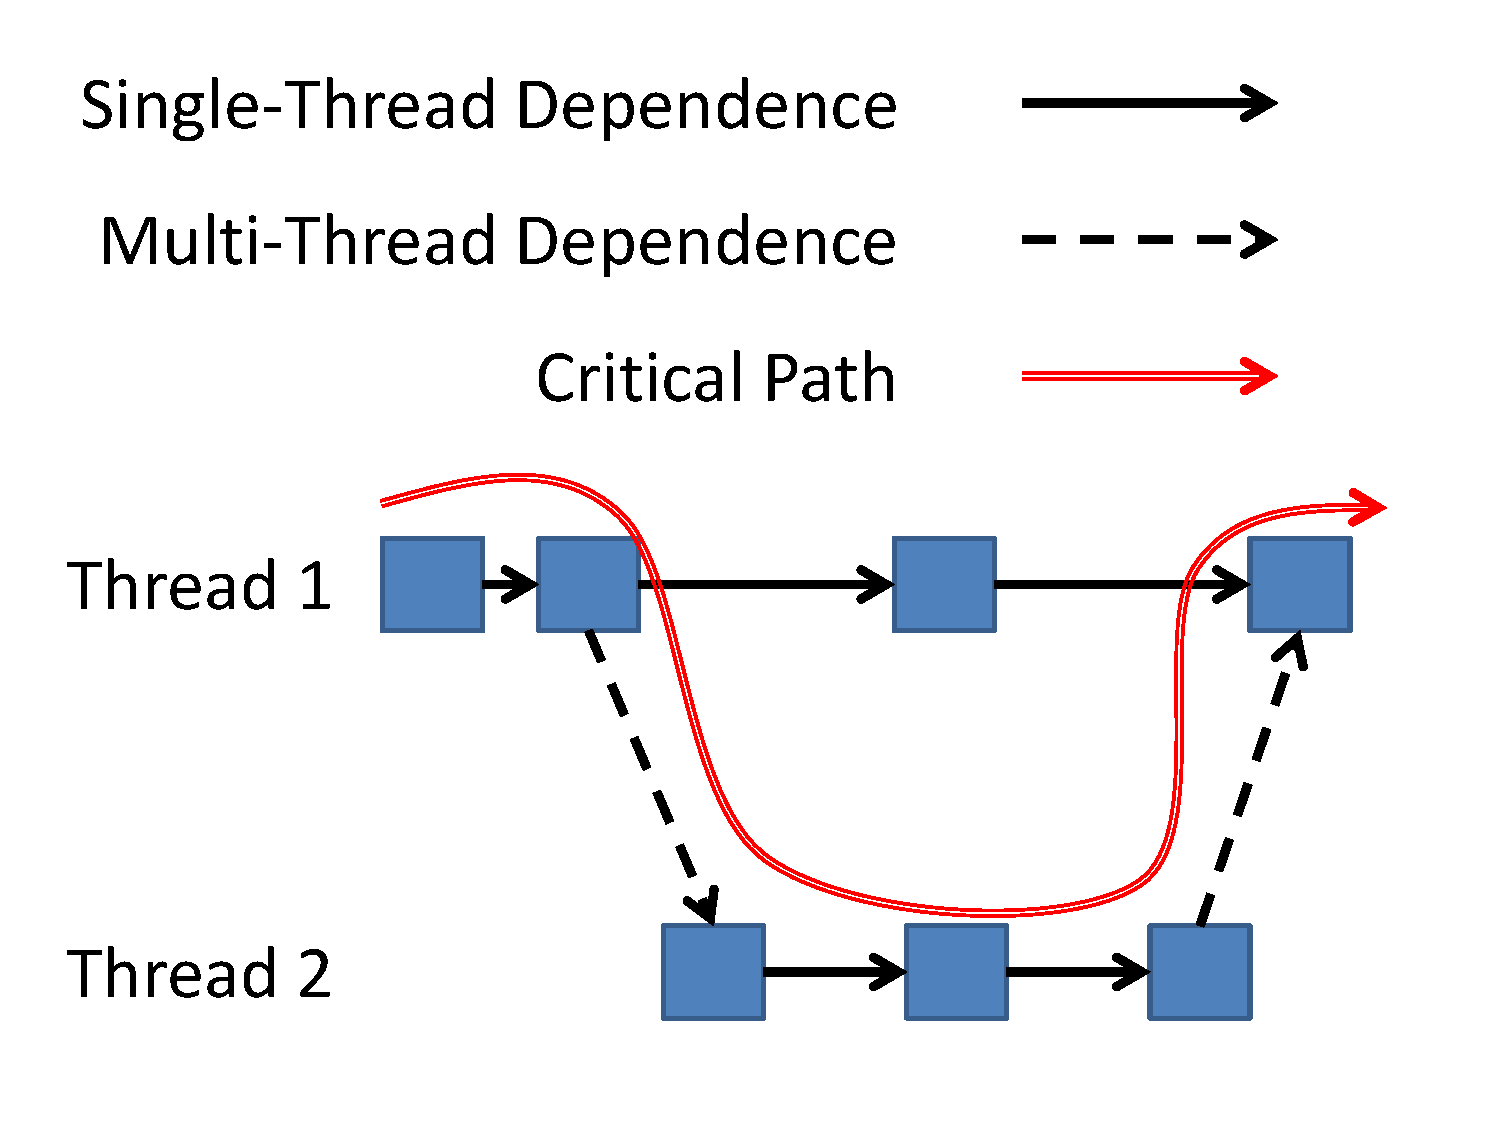
\includegraphics[width=.7\textwidth]{PMC/LPO.pdf}
\caption{\textbf{Local Persist Order.} LPO removes cross-thread persist dependencies, reducing persist critical path (PSC critical path traced in red).  Enforcing cross-thread dependencies requires explicit persist barriers.}
\label{figure:LPO}
\end{figure}

LPO potentially improves performance by minimizing the critical path of persist dependencies, shown in Figure~\ref{figure:LPO}.
Data sharing and the resulting cross-thread persist dependencies increase the critical path of persists.
The Figure displays the persist dependencies of two threads as well as shared dependencies.
Strict models, such as PSC, order persists between threads, increasing persist critical path (red arrow).
LPO, on the other hand, removes such dependencies, except where explicitly created by persist barriers.
Since threads persist independently, adding threads provides additional persist throughput, similarly to Symmetric Multi Threading (SMT), which provides memory parallelism on existing systems.
LPO, then, is an appropriate model where threads persist independently (no sharing occurs) or where memory sharing should not enforce persist order (such as batching).
However, the need to perform all persists in series within a thread remains a concern.
The Byte Addressable File System (BPFS) addresses intra-thread persist dependencies by introducing additional persist barriers.

\subsection{Byte Addressable Persistent File System}
\label{sec:PMC:PersistenceModels:BPFS}

The Byte Addressable Persistent File System (BPFS) \cite{ConditNightingale09} is the de-facto standard for existing persistent memory consistency models, used additionally by \cite{CoburnCaulfield11, FangHsiao11, VenkataramanTolia11}.
Threads persist by writing to the persistent address space, enforcing persist order via \emph{epoch barriers} which divide persists into \emph{epochs}.
Persists may not reorder across epoch barriers, but persists within an epoch are free to execute in parallel; BPFS provides a relaxed persistent consistency model (persists may occur out of program order) and uses barriers to enforce constraints.
BPFS additionally provides a hardware design, enforcing persist order with only cache modifications (little additional buffering or modifications to the memory system).
A table of epochs is kept in the cache of each CPU, with each cache line keeping track of its persist epoch number and process/thread ID (even cache lines with only volatile writes track persist epoch).
Persists buffered in the cache write back in the background, making sure that each epoch persists completely before starting to flush the next epoch.

Shared memory accesses enforce an ordering constraint between the epoch that produced the write and the epoch reading/overwriting that data.
This persist order is enforced strictly by stalling.
If at any point a thread overwrites a cache line from a previous persist epoch (even from the same thread), it stalls until the previous persist epoch completes persisting.
Further, if a thread reads a cache line from a persist epoch produced by a remote thread that has not yet persisted it also stalls until that epoch completes persisting (it does not stall if the reading thread is the same as the producing thread).
Persists within epochs write to the device in parallel, volatile execution proceeds ahead of persistent state, and cross-thread persist order is correctly enforced (at the cost of stalls).

\begin{figure}
\centering
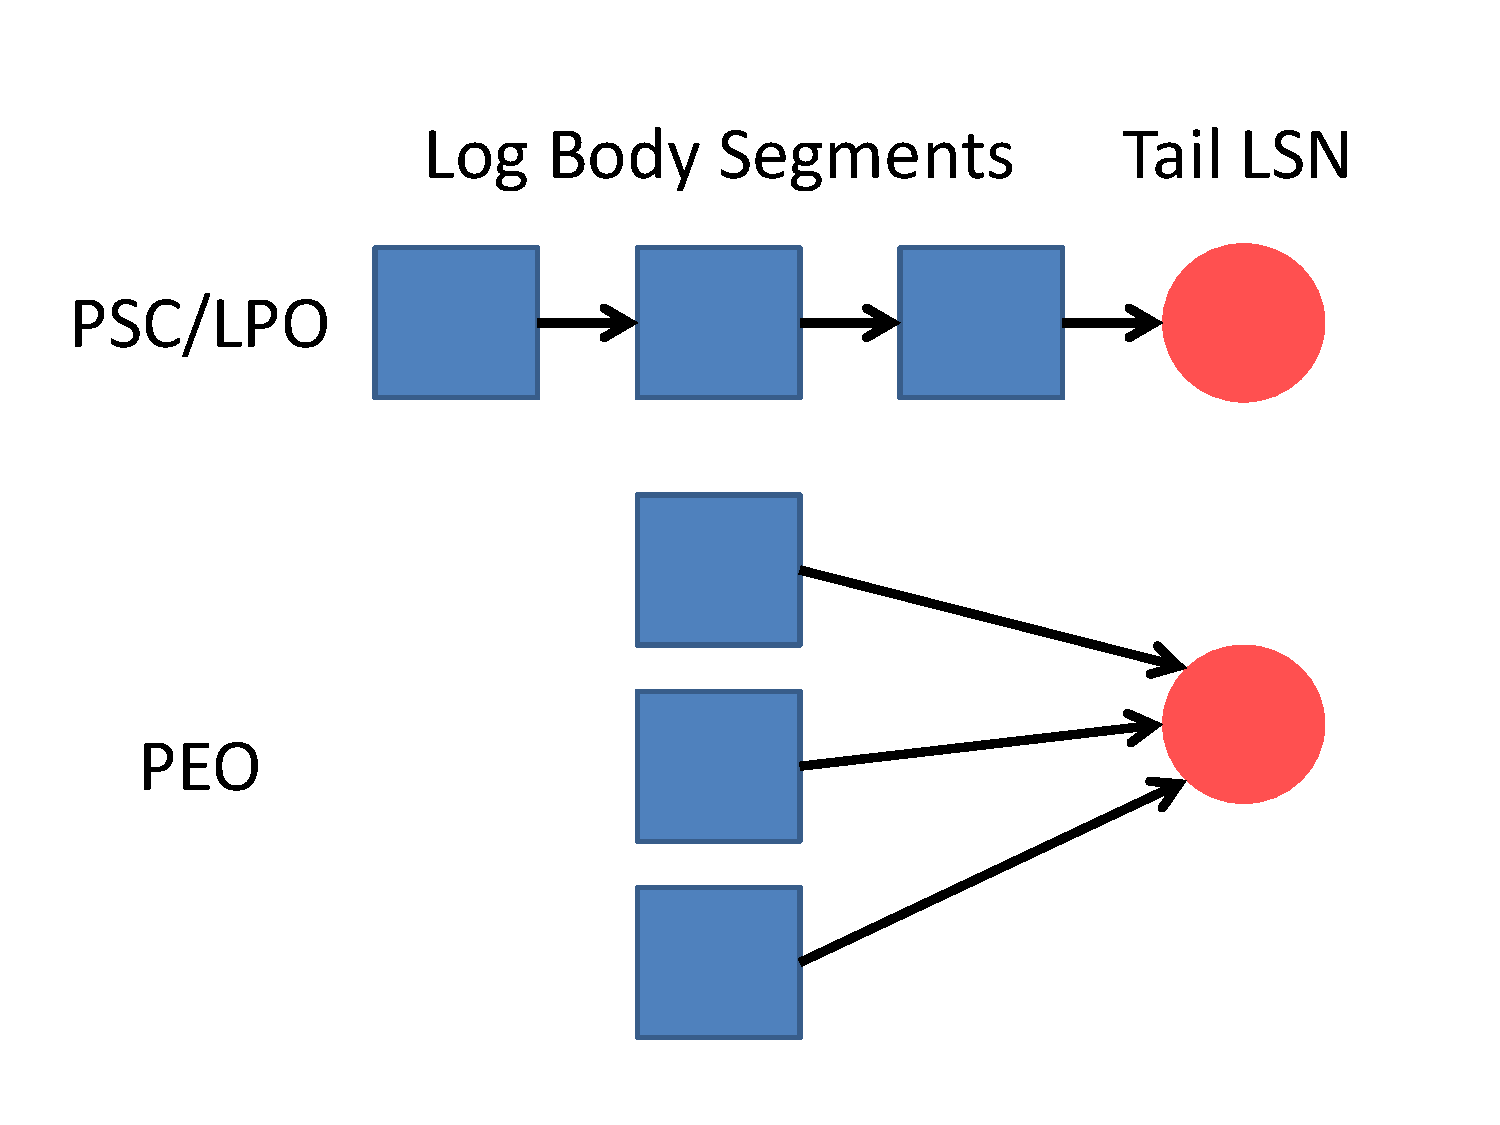
\includegraphics[width=.7\textwidth]{PMC/persist_wal.pdf}
\caption{\textbf{Partial Epoch Order.} PEO allows regions of NVRAM to persist in parallel while enforcing recovery correctness. \texttt{persist\_wal} persists entire log entry bodies in parallel using epochs.}
\label{fig:persist_wal_persist}
\end{figure}


Consider the ARIES log from Chapter~\ref{chap:OLTP_design}, demonstrated in \texttt{persist\_wal} (Figure~\ref{fig::Code}) with persist dependencies shown in Figure~\ref{fig:persist_wal_persist}.
Persisting a single entry requires first persisting the entry's body, followed by the tail LSN.
Most log entries are large (at least 100 bytes), containing information about the transaction, store, page, tuple, and action taken.
According to PSC and LPO all persists (8 byte segments) to the log entry body must occur in program order -- an unnecessary constraint that increases persist critical path.
Instead, BPFS allows the entire log entry body to persist in parallel, and guarantees that the body persists before the LSN using a persist barrier.

In consistency terms BPFS produces a total ordering between persist epochs that communicate through memory (Total Epoch Order -- TEO -- would be an appropriate name for this model).
This ordering resembles transactional memory -- producing a total order on memory transactions -- except BPFS does not provide concurrency control (conflicts are not detected and transactions can not roll back).
However, attempting to provide a total epoch order produces problems; races (data or synchronization) within BPFS epochs may result in deadlock.
The authors specifically prohibit races within their implementation, possibly recognizing that they introduce deadlocks.
However, preventing synchronization races restricts useful programming patterns.
I will demonstrate that the implementation as described allows deadlock and later provide example applications that make use of races.

{
\singlespacing
\newsavebox{\ThreadOne}
\begin{lrbox}{\ThreadOne}
  \begin{lstlisting}
Thread 1:

persist_bar
A = 1
B = 1
persist_bar
  \end{lstlisting}
\end{lrbox}

\newsavebox{\ThreadTwo}
\begin{lrbox}{\ThreadTwo}
  \begin{lstlisting}
Thread 2:

persist_bar
B = 2
A = 2
persist_bar
  \end{lstlisting}
\end{lrbox}

\begin{figure}[]
\centering
\subfigure{ \usebox{\ThreadOne} }
\hspace{1 in}
\subfigure{ \usebox{\ThreadTwo} }
\caption{\textbf{BPFS deadlock.} BPFS attempts to produce a total order on epochs.  Races within epochs create a cyclic order-dependence, resulting in deadlock.}
\label{fig:BPFS_deadlock}
\end{figure}
}

Consider Figure~\ref{fig:BPFS_deadlock}.
Each thread runs a single epoch with two persists to shared memory.
The second thread executes these persists in opposite order of the first.
If thread 1 writes to A at the same time thread 2 writes to B a deadlock occurs.
Thread 1 next attempts to write to B, fetching the cache line for B, and observes that thread 2 has not yet persisted, so thread 1's epoch must be ordered after thread 2's epoch.
Similarly, thread 2 attempts to write to A, ordering its epoch after thread 1's; a cycle has occurred, preventing forward progress.

This problem may occur even without data races or when persists have a total order.
Imagine that A and B on each thread are different variables, each protected by locks, but that thread 1's A (B) is on the same \emph{cache line} as thread 2's A (B).
Such \emph{false sharing} results in performance problems for existing volatile cache systems, but in the case of NVRAM and BPFS produces deadlock.
Furthermore, one might try to solve this problem by reordering thread 2's writes so that both thread 1 and thread 2 write in the same order, totally ordering the epochs (whoever accesses A first runs to completion while the other stalls).
However, relaxed consistency models allow the processor (or compiler) to reorder writes and persists within an epoch, arriving at the original problem.
In fact, it is not clear if instructions accessing only volatile data are permitted (or should be permitted) to reorder across epoch boundaries.
Next, A and B may represent synchronization races; consider atomic read-modify-write (such as compare-and-swap) to persistent address spaces.
BPFS, in assuming no races to persistent data, restricts the use of persistent locks.
Finally, certain data structures may specifically intend to allow races within persist epochs.
The \GroupCommit implementation described above, for example, requires threads to work concurrently towards a persistent state.

BPFS attempts to produce a total order of all epochs, producing deadlocks and preventing useful programming patterns.
I believe that the solution is to better define the interaction between persistence and the consistency model.
I next introduce a model strongly influenced by BPFS, that allows concurrent epochs to make forward progress at the cost of a slightly less intuitive interface.

\subsection{Partial Epoch Order}
\label{sec:PMC:PersistenceModels:PEO}

The third and final model relaxes persist order within a thread similarly to BPFS, but produces only a partial order of epochs between threads.
Partial Epoch Order (PEO) considers the epochs of two threads that communicate through memory to be \emph{concurrent}, and thus not ordered.
However, later epochs \emph{do} carry the dependence, allowing ordering of persists between threads while avoiding deadlock and allowing inter-thread persist concurrency.
When races do not occur within epochs PEO provides the same execution as BPFS.
As in LPO persists from concurrent epochs to the same address must have a total order, provided by the underlying consistency model.

{
\singlespacing
\newsavebox{\PEOThreadOne}
\begin{lrbox}{\PEOThreadOne}
  \begin{lstlisting}
Thread 1:

persist_bar (i)
persist A

persist_bar (ii)
persist B
write X

persist_bar (iii)
persist C
  \end{lstlisting}
\end{lrbox}

\newsavebox{\PEOThreadTwo}
\begin{lrbox}{\PEOThreadTwo}
  \begin{lstlisting}
Thread 2:

persist_bar (i)
persist D

persist_bar (ii)
read X
persist E

persist_bar (iii)
persist F
  \end{lstlisting}
\end{lrbox}

\begin{figure}[]
\centering
\subfigure{ \usebox{\PEOThreadOne} }
\hspace{1 in}
\subfigure{ \usebox{\PEOThreadTwo} }
\caption{\textbf{Partial Epoch Order (PEO).} PEO considers epochs in different threads containing a memory dependence to be concurrent.  This memory dependence does not enforce a persist order between the threads' epochs, but enforces this order on earlier and later epochs.  E must persist after A.}
\label{fig:PEO}
\end{figure}
}

Figure~\ref{fig:PEO} provides an example.
Two threads persist data and communicate through volatile object X, each persisting three epochs.
The threads communicate when thread 1, epoch (ii) writes to X, which thread 2 reads in its epoch (ii).
According to PEO, epochs (ii) of each thread are concurrent and do not enforce a persist order.
Thus, thread 1's persist to B may not necessarily occur before thread 2's persist to E.
However, epochs of thread 1 prior to (ii) must necessarily persist before epochs of thread 2 after (ii) -- When thread 2 reads a value from thread 1 it orders all later persist epochs after thread 1's earlier epochs.
Thread 1's persist to A must occur before thread 2's persist to F -- epochs containing shared memory accesses are concurrent, but later epochs carry the persist dependence.
The converse is not true -- thread 2's persist to D need not persist before thread 1's persist to C.
This model produces a partial ordering of persist epochs that all threads observe.

PEO removes the possibility of deadlock by relaxing persist order constraints.
However, PEO supports the same programming model as BPFS (a total epoch order).
Any program who's epochs contain only volatile races, or only persists (never both) will produce a total order on epochs containing shared memory persists, resulting in the same execution as BPFS.
Additionally, PEO's relaxed constraints allow advanced programming models such as batching.
Neglecting undo log (which must persist before store data) transactions in a batch may all execute within the same persist epoch.
Since these epochs are concurrent no persist order is enforced between persists of different threads.
When the batch ends transactions end their epoch and increment the semaphore/counter, as in Section~\ref{sec:PMC:PersistenceModels:LPO}.
The batch manager polls the counter until it matches the number of transaction threads, ends its own epoch, and invalidates the log.
In practice, transaction threads must use multiple epochs to order undo log persists before data persists; I would like to evaluate whether PEO provides sufficiently relaxed persist constraints or if other models (such as LPO) are required for batching performance.

It is unclear to me if volatile memory and non-memory instructions should be allowed to reorder with persist epoch barriers.
This will depend on the actual implementation, and if the hardware is able to easily distinguish persists from nonvolatile writes.
For example, thread 2's read to C in the previous example should be allowed to occur before the persist to B so long as the correct epoch order is enforced.
As persist barriers might be frequent, not allowing non-persistent instructions to reorder would limit the performance of \emph{volatile} memory instructions.

PEO provides effective single-thread persist parallelism while providing a relatively intuitive model for cross-thread persist-order dependencies.
PEO prevents deadlock and allows concurrent access to shared persistent memory spaces without enforcing a persist order.

\section{Conclusion}
\label{sec:PMC:Conclusion}

This chapter motivated the need for more precise persistent consistency models to allow greater persist performance and enforce correctness while providing an easy to program interface.
I proposed three new persistent consistency models and relate them to existing work.
While this chapter has focused on persistence semantics and the programming interface, the next chapter demonstrates common persistent data structures, focusing on potential performance concerns.


 %%%\chapter{Persistent Programming Patterns}
 %%%\label{chap:PMC_patterns}
 %%%The previous chapter looked at persistent memory programming from the perspective of consistency models and programming interfaces.
While necessary to define correct program behavior, I did not consider actual implementations or investigate specific optimizations.
This chapter investigates performance more directly, considering two simple persistent programming patterns -- a persistent log/buffer and a persistent linked list.
While I will describe how I expect the persistent memory consistency models from the previous chapters operate with each pattern, the point is to highlight potential performance bottlenecks and necessary optimizations.
I do not yet consider actual programming models or hardware to provide many of these optimizations.

Prior work has examined building data structures for NVRAM.
However, these works generally address other issues such as write endurance \cite{ChenGibbons11}, suggest data structures that intuitively fit NVRAM's programming interface without concern for performance \cite{VenkataramanTolia11}, or propose complicated software mechanisms to work around incomplete or inferior persistent consistency models \cite{FangHsiao11}.
While BPFS \cite{ConditNightingale09} takes a more holistic approach, their model falls short in terms of correctness, multi-threaded performance, and possibly single-thread performance, as I will show shortly.
I take a different approach, looking at useful data structures and potential performance concerns and using this insight to imagine new persistent consistency models and optimizations.

\section{Persistent Buffer}
\label{sec:PMC_patterns:Buffer}

\begin{figure}
\centering
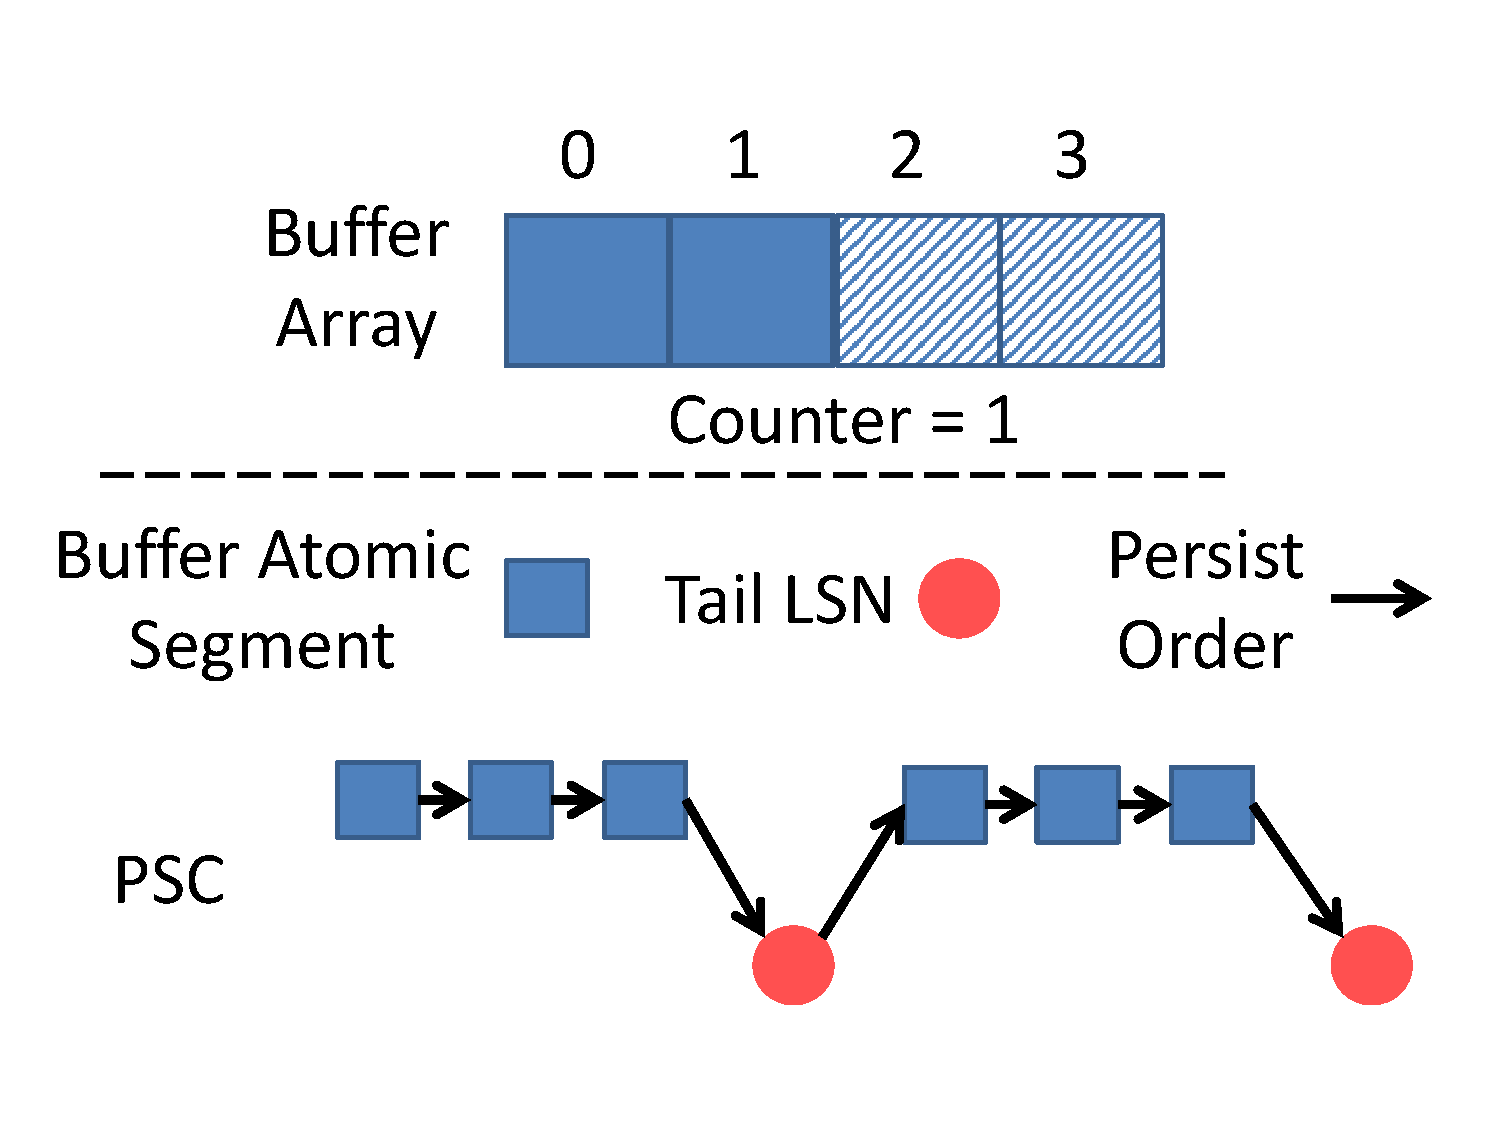
\includegraphics[width=\textwidth]{PMC_patterns/buffer.pdf}
\caption{Persistent buffer. The persistent buffer constists of a persistent array and counter (top).  The array holds persistent data.  The persistent counter marks the greatest persistent slot.  Persisting to the buffer under PSC places depdencies between writing buffer data and updating the counter, as well between persisting the counter and the next buffer persist, forming a chain (bottom).  This occurs both for single threaded and multithreaded use.}
\label{fig:buffer}
\end{figure}


I first discuss a persistent buffer, used as an OLTP database centralized log in \cite{FangHsiao11}.
The version presented here is a simplification of the implementation originally proposed, but illustrates the necessary performance concerns.
This log buffer contains a persistent data array as well as a persistent counter, marking the end of the valid, persistent region of the buffer, shown at the top of Figure~\ref{fig:buffer}.
In the example buffer slots 0 and 1 are persistent and valid, while slots 2 and 3 are not (0 and 1 will be recovered on failure).
For simplicity, I neglect details that require data to wrap around the end of the buffer and instead pretend that the valid region of the buffer always grows from the base offset of the buffer through the address marked by the counter.
Data are inserted into this buffer by acquiring a volatile lock on the structure, reading the counter to determine the next available address, persisting data to that address, and incrementing the counter by the size of the inserted data before releasing the lock.
For correctness, buffer data must persist before the new counter value persists, and all counter values must persist in order.
These dependencies guarantee that, on recovery, the valid portion of the buffer includes the base address through the address located in the persistent counter.

\cite{FangHsiao11} assumes the BPFS consistency model, noting that updates to the counter field will cause each thread to stall while the previous value persists.
Their work provides several complicated optimizations to 1) allow log entries from different threads to persist in parallel (by explicitly removing or re-ordering cross-thread dependencies) and (2) only persist intermediate values of the counter, removing a chain of persist dependencies that would otherwise limit throughput.
Such design improves performance but requires additional effort and is unintuitive.
Other persistent consistency models might enable these optimizations without the use of error-prone software implementations.
I qualitatively evaluation my three consistency models with this buffer, reasoning about persist critical path length per buffer insert.

\textbf{PSC.} Under PSC (recall, persistent sequential consistency) all persists to the buffer and counter form a dependence chain, shown at the bottom of Figure~\ref{fig:buffer}.
Every atomically persistable segment (8 bytes) of buffer data persists in serial, followed by the new value of the counter.
The next thread to insert into the buffer reads the counter, a shared variable, ordering all subsequent persists after persists of the previous insert.
Assuming log entries are 100 bytes on average, each insert requires 14 serial persists (13 to persist the log entry data, 1 to persist the counter).
If NVRAM persists take even 100ns (a conservative estimate), entries can only be inserted every 1.4\textmu s, on average (any faster and buffers will eventually fill).
This rate is significantly slower than the throughput of modern concurrent buffers, where cache invalidations take anywhere from 10s to 100s ns (multi-core to multi-socket, respectively).
Without relaxed persistent memory consistency models, NVRAM persists will necessarily create a throughput bottleneck.


\begin{figure}
\centering
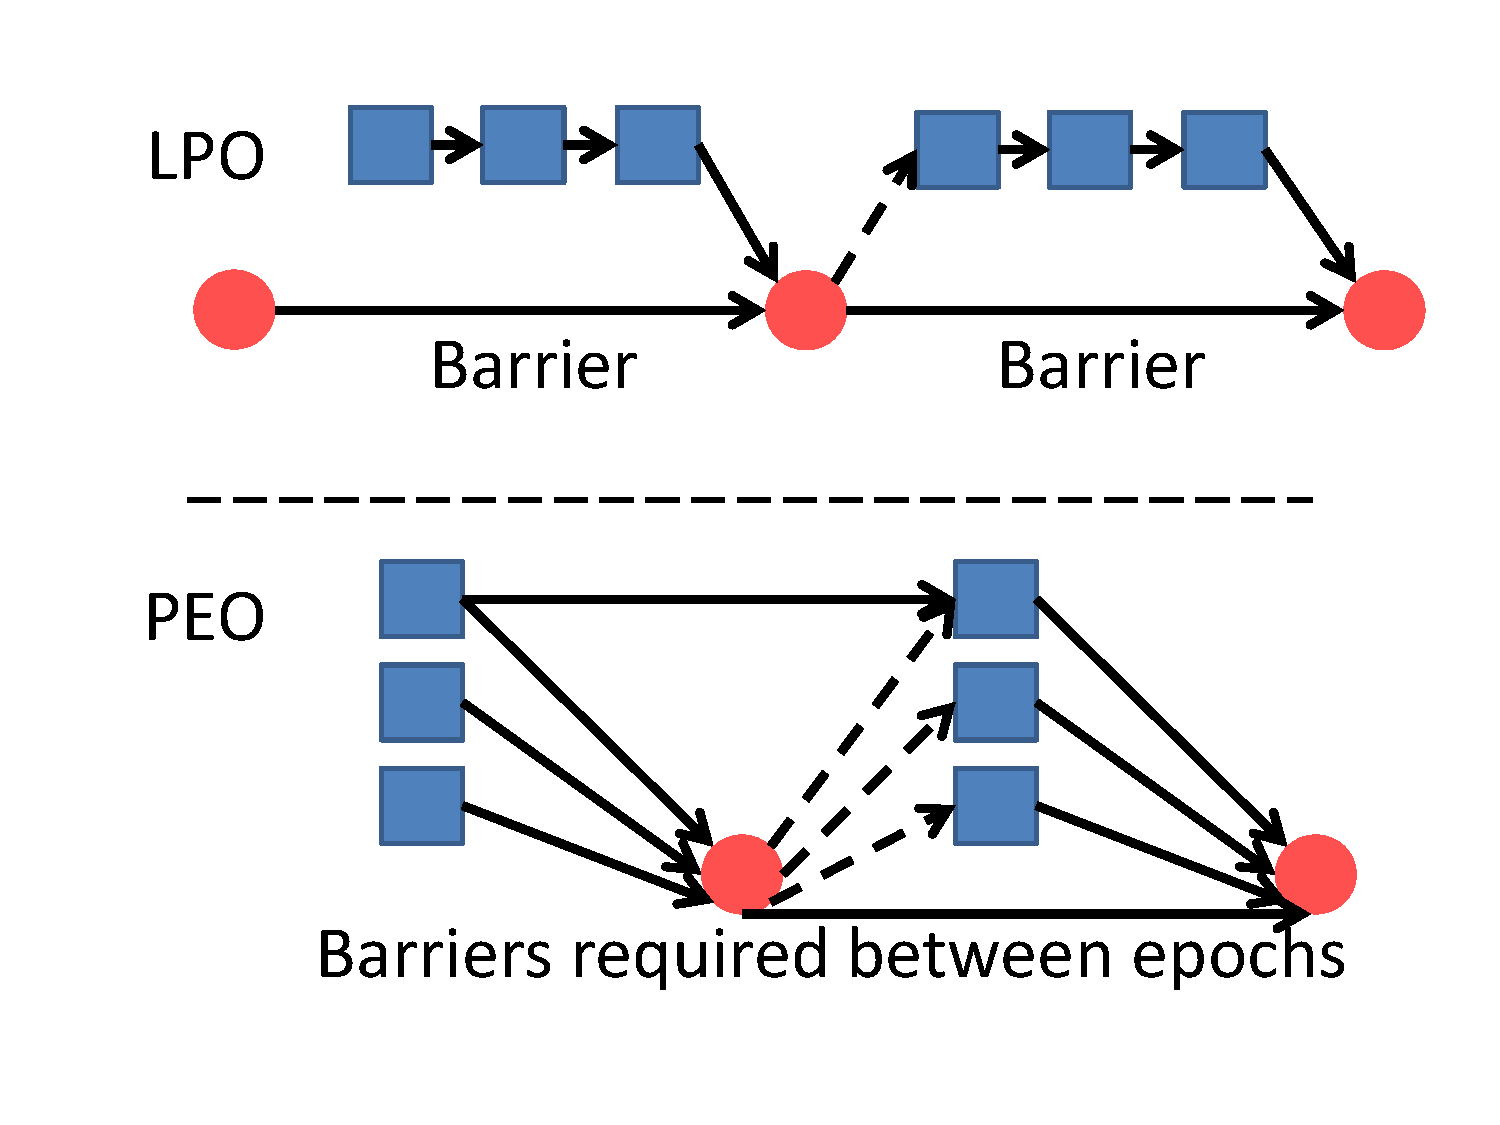
\includegraphics[width=.7\textwidth]{PMC_patterns/buffer_PEO_LPO.pdf}
\caption{\textbf{Buffer execution under LPO and PEO.}  LPO (top) removes persist dependencies between the counter value and subsequent buffer persists on other threads.  Dependencies remain when adjacent buffer inserts are from the same thread (dashed line).  PEO (bottom) allows buffer data to persist in parallel.}
\label{fig:buffer_PEO_LPO}
\end{figure}

\textbf{LPO.} Next I consider the relaxed persistent consistency models introduced in Section~\ref{sec:PMC:PersistenceModels}, starting with LPO.
Recall that LPO (local persist order) enforces program-order persist order within threads, but not cross-thread dependence order (barriers necessary).
Figure~\ref{fig:buffer_PEO_LPO} shows execution of LPO at the top.
Buffer persists continue to serialize and must persist before the counter, but there is no longer a dependence between the counter persisting and later buffer persists from other threads.
Counter values must still persist in-order, which will be enforced with a persist barrier or as a result of persists to the same memory address.
Dependencies \emph{do} exist between counter persists and subsequent buffer persists on the same thread, shown as a dashed line in the Figure.
If every log entry is inserted by a separate thread, LPO results in a persist critical path that involves only counter persists.
However, log entries within a single thread must persist in-order, limiting the throughput of each individual thread.
LPO is easy to program, as all persists within a thread occur-in order, and provides high throughput given sufficient buffering and a large number of threads to yield persist parallelism.

{
\singlespacing
\newsavebox{\BufferPEO}
\begin{lrbox}{\BufferPEO}
  \begin{lstlisting}
PEO:

persist_bar (i)
lock_acquire()
dest = buffer[counter] # reads counter
memcpy(buffer, entry) # persists buffer

persist_bar (ii)
counter += entry.size # persists counter
lock_release()
  \end{lstlisting}
\end{lrbox}

\newsavebox{\BufferTEO}
\begin{lrbox}{\BufferTEO}
  \begin{lstlisting}

TEO:

persist_bar (i)
lock_acquire()

persist_bar (ii)
dest = buffer[counter] # reads counter
memcpy(buffer, entry) # persists buffer

persist_bar (iii)
counter += entry.size # persists counter

persist_bar (iv)
lock_release()
  \end{lstlisting}
\end{lrbox}

\begin{figure}[]
\centering
\subfigure{ \usebox{\BufferPEO} }
\vspace{1 in}
\subfigure{ \usebox{\BufferTEO} }
\caption{\textbf{Buffer insert with PEO/TEO.} Pseudocode implements buffer insert with two persist barriers.  PEO's concurrent epochs allow epoch (ii) to persist in parallel with epoch (i) of the next insert operation. TEO simplifies persist-order reasoning, separating volatile races from persists.  PEO requires four barriers and introduces persist dependencies between persisting buffer data and the previous counter value.}
\label{fig:buffer_PEO_pseudocode}
\end{figure}
}

\textbf{PEO.} The bottom of Figure~\ref{fig:buffer_PEO_LPO} displays buffer execution for PEO -- partial epoch order.
Partial epoch order allows single-thread persists to occur in parallel by placing them in epochs.
Epochs across threads are ordered (or considered concurrent) according to the consistency model and memory sharing.
PEO allows buffer data to persist in parallel, and removes ordering constraints between buffer persists and the previous counter persist from another thread (epochs are concurrent -- see Figure~\ref{fig:buffer_PEO_pseudocode}).
However, buffer persists are ordered after buffer persists of the previous insert (solid arrows in the Figure), and ordered after counter persists from the same thread (dashed arrows in the Figure).

Assuming subsequent inserts occur from different threads the persist critical path forms a chain of only one persist epoch per insert (either through the counters or through the buffer persists).
Using our earlier assumptions, this model allows inserts every 100ns on average.
Such delays are similar to invalidation delays in modern multi-socket CPU systems, but NVRAM may require more than 100ns per serialized persist.
Furthermore, PEO requires frequent persist barriers, placing a burden on the programmer.
While these epoch barriers are deemed intuitive, they are not as easy to use as sequential consistency (no barriers required) and are more complicated to reason about with multi-threading (as evident by BPFS allowing deadlocks).

Reasoning about concurrent epochs is quite difficult.
I provide a second implementation of buffer insert under PEO (Figure~\ref{fig:buffer_PEO_pseudocode}, bottom) that allows a total order of persist epochs (as intended by BPFS).
Epochs in this implementation have either volatile races (lock/release) or persists, not both.
Additionally, a barrier is still required to guarantee that buffer data persists before updating the counter.
This implementation, while more obviously correct, increases persist critical path by introducing a dependence between counter persist and the next buffer data persist (the dashed arrow of Figure~\ref{fig:buffer_PEO_LPO} occurs even for cross-thread dependencies).


\begin{figure}
\centering
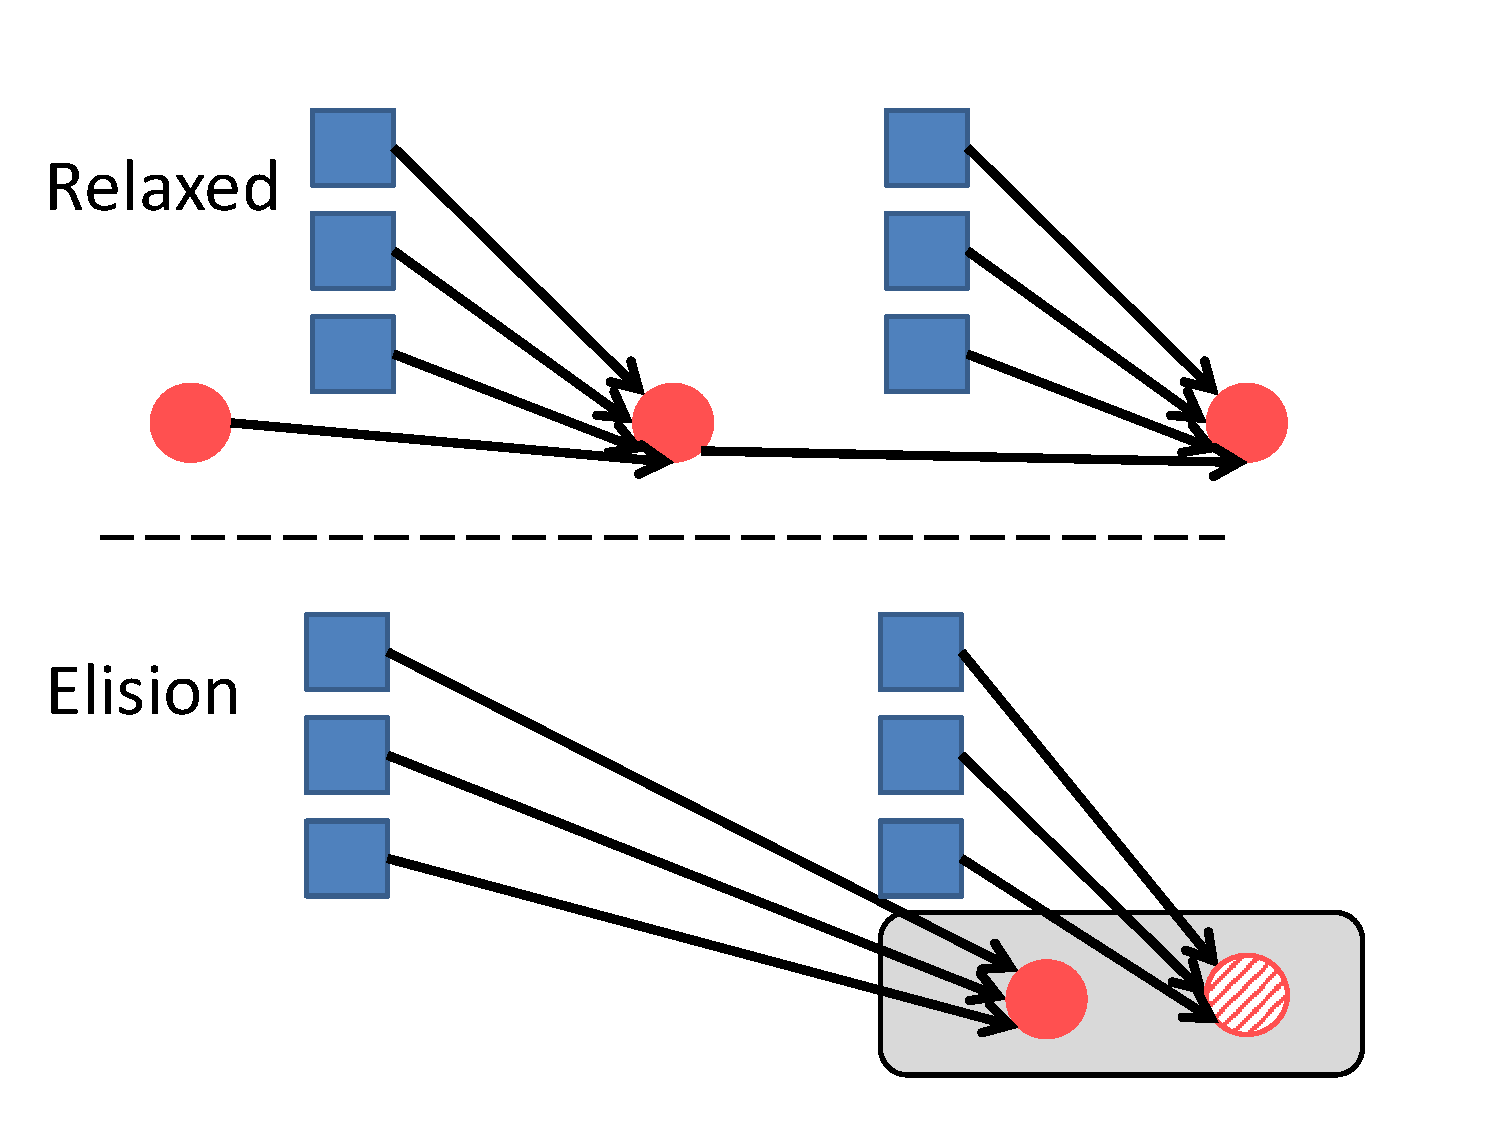
\includegraphics[width=.7\textwidth]{PMC_patterns/buffer_relaxed_elision.pdf}
\caption{\textbf{Buffer execution under relaxed persistent consistency.}  Relaxing persistent consistency removes unnecessary cross-thread dependencies (as in LPO), allows epochs to persist in parallel (as in PEO), and removes unnecessary serial epoch dependencies within threads (top).  Epochs/dependencies are elided by persisting only select counter values (bottom).}
\label{fig:buffer_relaxed_elision}
\end{figure}

\textbf{Relaxed persistent consistency.}
Finally, I imagine a relaxed consistency model for this buffer, shown in Figure~\ref{fig:buffer_relaxed_elision} (top).
I will not describe the semantics of this model, but rather the desired persist dependencies.
Like PEO buffer data persists in parallel.
Like LPO there are no dependencies between counter persists subsequent buffer persists.
In fact, this is true even for single-threaded use.
Doing so requires more complicated barriers that do not impose serial dependencies between epochs, but instead allow precise, possibly named dependencies.
For example, a barrier may enforce that a given epoch depends only on the previous epoch from the same thread, and no other epochs regardless of thread communication or data dependencies.
Such a barrier would allow a programmer to persist buffer data and guarantee that buffer persists never serialize after counter persists.

I introduce an additional optimization to the relaxed consistency model, leveraging the insight from \cite{FangHsiao11} that not all values must persist, shown at the bottom of Figure~\ref{fig:buffer_relaxed_elision}.
Persistent memory consistency models describe the set of \emph{allowable} persistent states, yet not every allowable state must actually persist.
Since the counter is atomically persistable (8 bytes), the memory system may defer persisting new values of the counter.
Once the buffer data for two (or more) adjacent log entries successfully persist, the counter value for the last entry persists, implicitly persisting all intermediate counter values at once and validating the log entries, eliding persist epochs entirely.
By recognizing that the counter variable is atomically persistable and exists in an epoch by itself, we might imagine a new epoch barrier that restricts the epoch to a single persist of atomic persist size.
This persist will defer, hoping to coalesce with similar persist epochs.
A new value will eventually persist, but may skip any intermediate values so long as all the coalesced persist epochs' dependencies are satisfied.
The result is that the persist critical path is now bounded to a constant -- persists should never limit the throughput of this buffer (assuming large but finite buffers).

More generally, persist dependencies form a schedule or DAG, with persist epochs forming nodes in the graph and epoch dependencies forming edges.
Nodes in the DAG may be combined into an elision super node (combining all the nodes' persists) so long as 1) all persists in the super node fit in an atomically persistable size, 2) combining nodes retains the DAG (no cycles introduced), and 3) the super node inherits all dependencies of its member nodes, and all nodes that previously depended on the super node's member nodes now depend on the super node.
An interesting prospect is that as NVRAM technologies progress, the atomically persistable size may increase (say, from 8 bytes to 64 bytes).
Larger atomic persists allow additional persist epochs to coalesce into super nodes, decreasing persist critical path, possibly without intervention from the user.
It remains unclear if this property should be leveraged by hardware or in the consistency model, if at all.

\section{Persistent Linked List}
\label{sec:PMC_patterns:LinkedList}

\begin{figure}
\centering
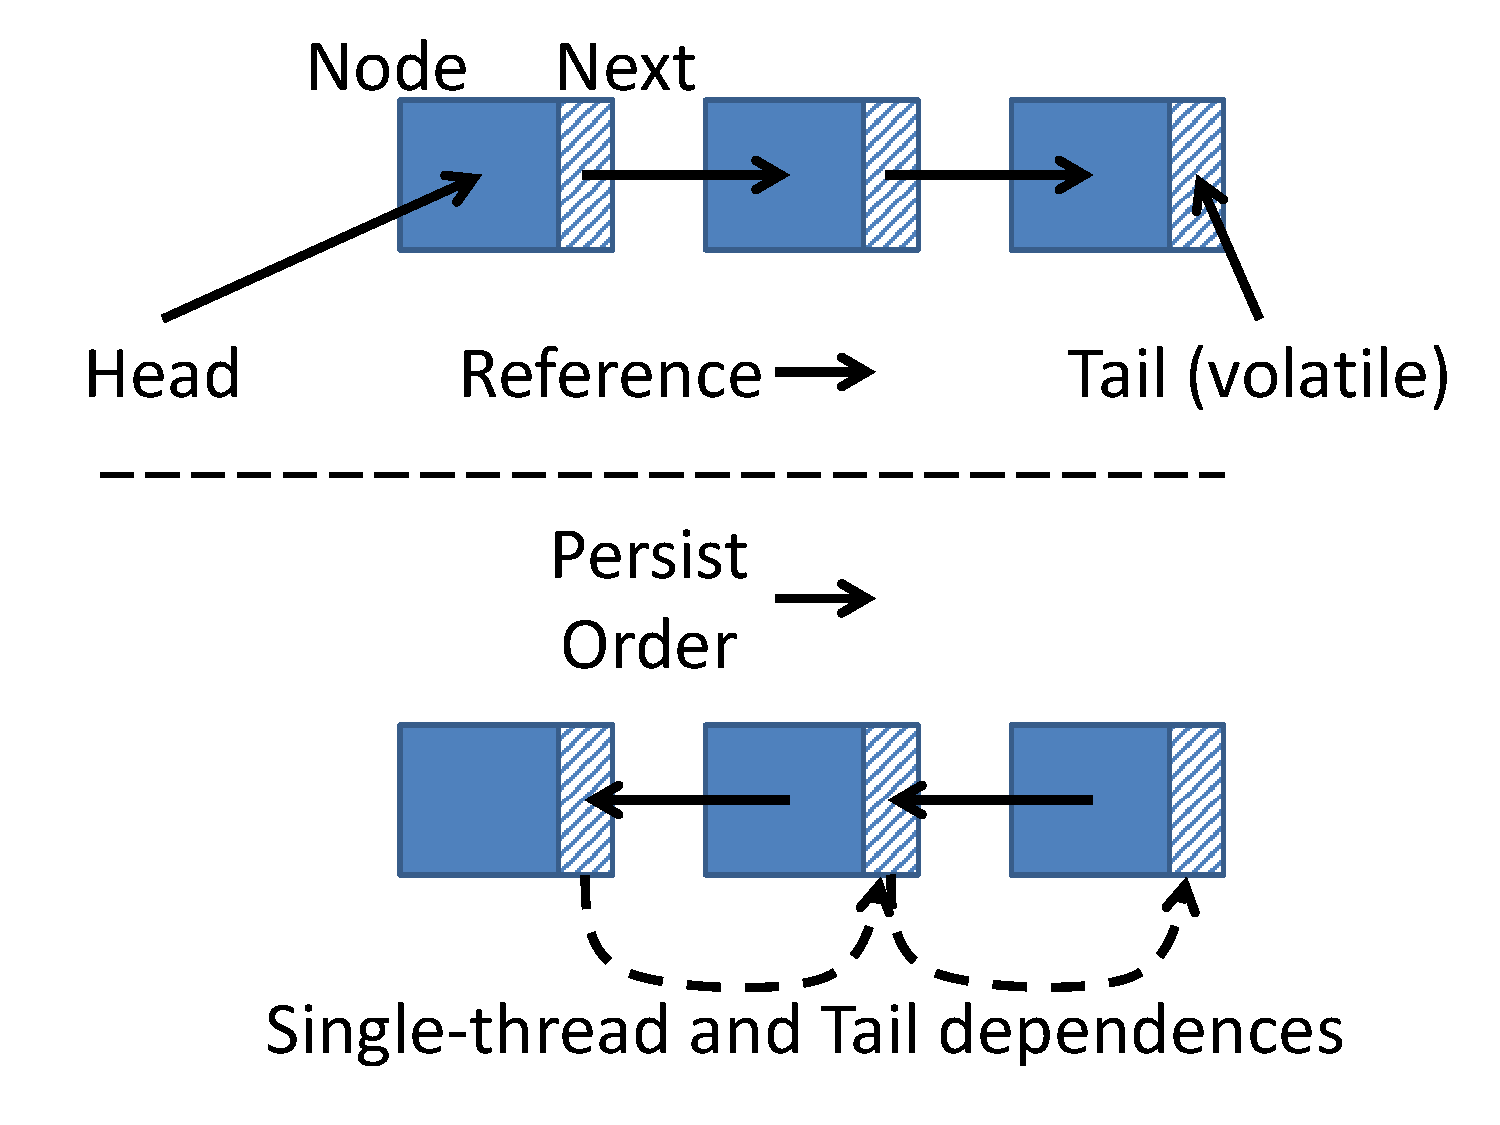
\includegraphics[width=.7\textwidth]{PMC_patterns/linkedlist.pdf}
\caption{\textbf{Persistent linked list.}  The linked list constains nonvolatile Head pointer, volatile Tail pointer, and nodes (data -- solid square; \emph{next} reference -- patterned box).  Nodes persist in parallel (data must still persist before references).  Dashed lines show unnecessary dependencies enforced by strict persistent consistency models, forming a dependence chain.  The valid list is determined at recovery by traversing from Head to the last valid node reference.  Implementing efficient sync remains a challenging.}
\label{fig:LinkedList}
\end{figure}


Finally, I consider a persistent linked list, shown in Figure~\ref{fig:LinkedList}.
The linked list contains a persistent Head reference, persistent nodes (each containing a \emph{next} reference), and a volatile Tail reference to quickly find the end of the list for insertion (although I assume that at recovery the list will only be traversed from the Head).
Unlike the persistent buffer, where log entries persist in parallel and the counter is overwritten, the linked list does not overwrite any values as new nodes are added.
For correctness, node data must persist before the node \emph{next} reference pointing to that data.
However, strict persistent consistency models will enforce that all nodes persist in the order that they are inserted into the list (dependencies shown as dotted lines in the bottom of the Figure).
Ignoring sync operations briefly, it would be correct to allow nodes to persist in parallel (references persisting after associated data), and simply determine the persistent and valid portion of the list at recovery.
Doing so bounds the persist critical path to a constant.
However, there is now no efficient way to sync the list short of traversing the entire list again, ordering the sync after all persists within the traversal.
This is an interesting design for persistent lists that require high throughput, rarely sync, and prefer linked lists (perhaps to insert in the middle).
Faster, more efficient, yet intuitive sync design remains an interesting challenge.

\section{Conclusion and Future Work}
\label{sec:PMC_patterns:Conclusion}

This chapter considered persistent memory consistency from a performance perspective.
I investigated two simple programming patterns, considering how my proposed persistent consistency models might perform and imagining additional optimizations, separate from the programming model, necessary to increase persistent data structure throughput.

For the future, I would like to develop these ideas and design some sort of methodology to support my claim that persistent memory consistency models are a necessary tool and require further investigation.
To start, I would like to implement the above data structures, annotating the code with persist dependencies and using a timing model similar to the one outlined in Section~\ref{sec:OLTP_design:Methodology}.
Additionally, I would consider implementing these models in Shore-MT.
Finally, I will consider additional models if the described models do not provide sufficient performance, or I discover that other models provide sufficient performance and are easier to program for.
I am especially interested in determining if models stricter than BPFS (fewer barriers) provide sufficient performance.
I plan to submit a paper based on these ideas to this upcoming ISCA, November 2013, and defend next year (2014).

Future work (hopefully outside the scope of my thesis) might consider an evaluation framework that does not require code annotation -- programs are written truly assuming consistency models and executed via simulation.
Additionally, future work will consider actual hardware implementations of useful persistent memory consistency models.


 \chapter{Memory Persistency}
 \label{chap:Persistency}
 The previous chapters considered how to design recoverable software assuming various latencies for persist barriers.
However, the memory system implementation remained unspecified, and ultimately will determine performance.
The remainder of this dissertation in turn investigates programming interfaces for persistent memory and how the interface might affect system performance.

This chapter motivates and defines \emph{memory persistency}, a framework for reasoning about and enforcing the order of persist operations.
The following chapters propose and evaluate example persistency models.
This work was completed in collaboration with my advisor, Thomas F. Wenisch, and Professor Peter M. Chen.
Refer to Section~\ref{sec:Background:MemoryConsistency} for a discussion of memory consistency and consistency models.

\section{Introduction}
\label{sec:Persistency:Intro}

Emerging nonvolatile memories (NVRAM) promise high performance recoverable systems.
These technologies, required as replacements for Flash and DRAM as existing technologies approach scaling limits \cite{LeeIpek09}, pair the high performance and byte addressability of DRAM with the durability of disk and Flash memory.
Future systems will place these devices on a DRAM-like memory bus, providing systems with throughput similar to DRAM, yet recoverability after failures.

However, ensuring proper recovery requires constraining the order of NVRAM writes.
Existing DRAM architectures lack the interface to describe and enforce write ordering constraints; ordering constraints that arise from memory consistency requirements are usually enforced at the processor, which is insufficient for failure tolerance with acceptable performance.
Recent work has suggested alternative interfaces to enforce NVRAM write order and guarantee proper recovery, for example durable transactions and persist barriers \cite{VolosTack11, ConditNightingale09}.
While intuitive and suitable to specific applications, I wish to investigate a more general framework for reasoning about NVRAM write ordering including mechanisms for expressing write constraints that are independent of specific concurrency control mechanisms.

Instead, I recognize that the problem of constraining NVRAM write concurrency resembles memory consistency.
Memory consistency restricts the visible order of loads and stores (equivalently, allowable visible memory states) between processors or cores, allowing operations to reorder so long as expected behavior is guaranteed.
Memory consistency models provide an interface and set of memory order guarantees for the programmer, but separate the implementation; several distinct implementations may fulfill the same memory consistency model, allowing sophisticated optimization (e.g., speculation \cite{Blundell09,Wenisch07,Ceze07,Gniady99,Ranganathan97}).
Relaxing the memory consistency model places an additional burden on the programmer to understand the model and insert the correct annotations, but often allows greater performance.

I introduce \emph{Memory Persistency}, a framework motivated by memory consistency to provide an interface for enforcing the order in which NVRAM writes become durable, an operation referred to as a ``persist'' (as in previous chapters).
Memory persistency prescribes the order of persist operations with respect to one another and loads and stores, and allows the programmer to reason about guarantees on the ordering of persists with respect to system failures.
The memory persistency model relies on the underlying memory consistency model and volatile memory execution to define persist ordering constraints and the values written to persistent memory.

In the following chapters, I define memory persistency, describe the design space of memory persistency models, and introduce and evaluate several new persistency models.
Much like consistency, I identify \emph{strict} and \emph{relaxed} classes of persistency models.
Strict persistency relies on implicit guarantees to order persists and couples persistent semantics to the underlying memory consistency model: any two stores to the persistent address space that are guaranteed to be observed in a well-defined order from the perspective of a third processor imply well-ordered NVRAM writes.
Thus, the same mechanisms the consistency model provides a programmer to enforce order for stores also enforce order for the corresponding persists. 
Alternatively, relaxed persistency separates volatile and persistent memory execution, allowing the order of persist operations to differ from the order in which the corresponding stores become visible.
Relaxed persistency facilitates concurrent persists even when volatile memory operations become visible according to sequential consistency.
Memory persistency further provides an interface for uniprocessors, which may not ordinarily order stores, to specify persist ordering constraints.
While separating memory consistency and persistency provides advantages to programmability and performance, it also introduces new challenges, as separate annotations define allowable reorderings for visibility and persistence of writes to the persistent address space.

Using this framework, I introduce successively relaxed memory persistency models and demonstrate how programmers can exploit the reorderings they allow through several example implementations of a thread-safe persistent queue.
I demonstrate that conservative memory consistency (such as sequential consistency) with strict persistency must rely on thread parallelism to enable NVRAM write concurrency.
On the other hand, relaxed persistency allows high instruction execution performance, NVRAM write concurrency, and simplified data structures.

Finally, I evaluate my memory persistency models and queue designs.
Just as with memory consistency, a memory persistency model is defined separately from its implementation.
Instead of assuming specific storage technologies and memory system implementations, I measure NVRAM write performance as the critical path of persist ordering constraints, assuming that NVRAM writes form the primary system bottleneck and that practical memory systems effectively use available concurrency.
I demonstrate that relaxed persistency models substantially improve write-concurrency over sequential consistency with strict persistency; for a 500ns NVRAM write latency, these concurrency gains improve performance to the throughput limit of instruction execution---as much as 30x speedup over strict persistency.

\section{Memory Persistency Goals}
\label{sec:Persistency:Goals}

Correct recovery of durable systems requires persists to observe some set of happens-before relations, for example, that persists occur before an externally observable action, such as a system call.  
However, I expect NVRAM writes to be much slower than writes to volatile memory.
Provided the minimal set of happens-before relations is observed, the gap between volatile execution and NVRAM write performance can be shrunk by optimizations that increase concurrency. 
I am interested in defining persistency models that create opportunities for two specific optimizations: \emph{persist buffering}, and \emph{persist coalescing}.
Additionally, I intend to propose persistency models that maximize instruction execution throughput and preserve existing thread synchronization patterns, including synchronization to the persistent address space.

\textbf{Persist Buffering.}
Buffering durable writes and allowing thread execution to proceed ahead of persistent state greatly accelerates performance \cite{ConditNightingale09}.
Such buffering overlaps NVRAM write latency with useful execution. 
To be able to reason about buffering, I draw a distinction between a ``store'', the cache coherence actions required to make a write (including an NVRAM write) visible to other processors, and a ``persist'', the action of writing durably to NVRAM.
Buffering permits persists to occur asynchronously.  

Ideally, persist latency is fully hidden and the system executes at native volatile memory speed.
With finite buffering, performance is ultimately limited by the slower of the average rate that persists are generated (determined by volatile execution rate) and the rate persists complete.
At best, the longest chain (critical path) of persist ordering constraints determines how quickly persists occur (at worst, constraints within the memory system limit persist rate, such as bank conflicts or bandwidth limitations).
In defining persistency models, my goal is to admit as much persist concurrency as possible by creating a memory interface that avoids unnecessary constraints.
Persistency model implementations might buffer persists in existing store queues and caches or via new mechanisms, such as buffers within NVRAM devices.

\textbf{Persist Coalescing.}
I expect that NVRAM devices will guarantee atomicity for persists of some size (e.g., eight-byte atomicity \cite{ConditNightingale09}).
Persists to the same atomically persistable block may coalesce (be performed in a single persist operation) provided no happens-before constraints are violated. 
Persist coalescing creates an opportunity to avoid frequent persists to the same address, and allows caching/buffering mechanisms to act as bandwidth filters \cite{Goodman83}.
Coalescing also reduces the total number of NVRAM writes, which may be important for NVRAM devices that are subject to wear.
Larger atomic persists facilitate greater coalescing.
Similarly, persistency models that avoid unnecessary ordering constraints allow more coalescing. 

While similar gains may be achieved through software (by caching values in nonpersistent memory and precisely controlling when they are persisted), I believe that hardware-enabled persist coalescing is an important feature.
Automatic coalescing relieves the programmer of the burden to manually orchestrate coalescing and specify when persists occur via copies.
Additionally, automatic coalescing provides backwards compatibility by allowing new devices to increase the size of atomic persists to improve coalescing performance.
I do not consider specific hardware implementations to detect when persists may coalesce, but assume that it is an important property of high performance persistent memory systems.

\textbf{Minimizing non-persistent overheads.}
Existing data structures intended for volatile memory must be modified for persistent memory, for example, by adding logging or copy-on-write to make persistent updates atomic with respect to recovery.
Additionally, new synchronization delays will be introduced with strict persistency if store barriers are inserted to enforce persist order (under strict persistency store barriers are also persist barriers).
Data structures modified to be recoverable will ultimately run more slowly even on existing volatile memory systems.
The persistency model will determine how invasive these software transformations are as well as the extent of their performance impact, thus motivating the need to explore the design space of persistency models.

Finally, persistent memory systems must continue to support advanced thread synchronization mechanisms.
One area that has not yet been investigated is synchronization to persistent memory, including locks, atomic read-modify-write (e.g., add, exchange, test-and-set), and compare-and-swap.
While this work does not attempt to use these primitives, I intend to introduce persistency models that properly define their with NVRAM.
Extending existing consistency models provides a framework to define persistent behavior for atomic synchronization primitives.

\section{Memory Persistency}
\label{sec:Persistency:Persistency}

Recovery mechanisms require specific orders of persists.
Failure to enforce this order results in data corruption.
A persistency model enables software to label those persist-order constraints necessary for recovery-correctness while allowing concurrency among other persists.
As with consistency models, my objective is to strike a balance between programmer annotation burden and the amount of concurrency (and therefore improved performance) the model enables.

I introduce memory persistency as an extension to memory consistency to additionally order persists and facilitate reasoning about persist order with respect to failures.
Conceptually, I reason about failure as a \emph{recovery observer} that atomically reads all of persistent memory at the moment of failure.
Ordering constraints for correct recovery thus become ordering constraints on memory and persist operations as viewed from the recovery observer.
With this abstraction, one may apply the reasoning tools of memory consistency to persistency---any two stores to the persistent memory address space that are ordered with respect to the recovery observer imply an ordering constraint on the corresponding persists.
Conversely, stores that are not ordered with respect to the observer allow corresponding persists to be reordered or performed concurrently.
The notion of the recovery observer implies that even a uniprocessor system requires memory persistency as the single processor must still interact with the observer (i.e., uniprocessor optimizations for cacheable volatile memory may be incorrect for persistent memory).

Much like consistency models, there may be a variety of implementations for a particular memory persistency model.
Like the literature on consistency, I separate model semantics from implementation; my focus in this work is on exploring the semantics.
While I do discuss some implementation considerations, I omit details and leave system design and optimization to future work.
I divide persistency models into \emph{strict} and \emph{relaxed} classes, and consider each with respect to the underlying consistency model.

\subsection{Strict Persistency}

The most intuitive memory persistency model is \emph{strict persistency.}
Strict persistency couples memory persistency to the memory consistency model, using the existing consistency model to specify persist ordering.
Minimal programmer annotations are required---while processor memory barriers are unnecessary, compiler barriers prevent optimizations that interfere with proper recovery.
Under strict persistency, the recovery observer participates in the memory consistency model precisely as if it were an additional processor.  
Hence, any store ordering that can be inferred by observing memory order implies a persist ordering constraint.
Persist order must match the (possibly partial) order in which stores are performed in a particular execution.
 
Conservative consistency models, such as SC, do not allow stores from each thread to reorder from the perspective of other threads; all stores, and therefore persists, occur in each thread's program order.
However, such models can still facilitate persist concurrency by relying on thread concurrency (stores from different threads are often concurrent).
On the other hand, relaxed consistency models, such as RMO, allow stores to reorder.
Using such models it is possible for many persists from the same thread to occur in parallel.
However, the programmer is now responsible for inserting the correct memory barriers to enforce the intended behavior, as is currently the case for shared-memory workloads.

Strict persistency unifies the problem of reasoning about allowable memory order and allowable persist order (equivalently, allowable persistent states at recovery); a program that is correctly synchronized with respect to the consistency model is also correctly labeled with respect to the recovery observer.
However, directly implementing strict persistency implies frequent stalls---consistency ordering constraints (e.g., at every memory operation under SC and at memory barriers under RMO) stall execution until NVRAM writes complete. 
A programmer seeking to maximize persist performance must rely either on relaxed consistency (with the concomitant challenges of correct program labeling), or must aggressively employ thread concurrency to eliminate persist ordering constraints.
As I will show, decoupling persistency and consistency ordering allows recoverable data structures with high persist concurrency even under SC.

I introduce one important optimization to strict persistency, \emph{buffered strict persistency}, which can improve performance while still guaranteeing strict ordering of persists and visible side effects.  
Buffered strict persistency allows instruction execution to proceed ahead of persistent state, thus allowing overlap of volatile execution and serial draining of queued persist operations.
In terms of the recovery observer, buffered strict persistency allows the observer to lag arbitrarily far behind other processors in observing memory order.
Therefore, the persistent state of the system corresponds to some prior point in the observable memory order.
As side effects may otherwise become visible prior to earlier persists, I additionally introduce a \emph{persist sync} operation to synchronize instruction execution and persistent state (i.e., require the recovery observer to ``catch up'' to present state). 
The persist sync allows the programmer to order persists and non-persistent, yet visible, side effects.

\subsection{Relaxed Persistency}

Strict persistency provides mechanisms to reason about persist behavior using pre-existing memory consistency models.
However, memory consistency models are often inappropriate for persist performance.
Conservative consistency models such as SC and TSO serialize the visible order of stores; while high performance implementations of these models exist for volatile instruction execution \cite{Singh12,Lin12}, the high latency of NVRAM persists suggests that more relaxed persistency models may be desirable.

I decouple memory consistency and persistency models via \emph{relaxed persistency.}
Relaxed persistency loosens persist ordering constraints relative to the memory consistency model---that is, the visible order of persists (from the perspective of the recovery observer) is allowed to deviate from the visible order of stores.
Relaxing persistency requires separate memory consistency and persistency barriers.
Memory consistency barriers enforce the visibility of memory operation ordering with respect to other processors, while memory persistency barriers constrain the visible order of persists from the perspective of only the recovery observer.

Relaxing persistency allows systems with conservative consistency, such as SC, to improve persist concurrency without requiring additional threads or complicating thread communication.
In later chapters I introduce and explore several relaxed persistency models under SC.

Simultaneously relaxing persistency and consistency allows both the visibility of loads and stores to reorder among processors, and further allows the order of persists to differ from the order of stores.
An interesting property of such systems is that memory consistency and persistency barriers are decoupled---store visibility and persist order are enforced separately---implying that persists may reorder across store barriers and store visibility may reorder across persist barriers.
Separating store and persist order complicates reasoning about persists to the same address, as I show next.

\subsection{Relaxed Persistency and Cache Coherence}
Under SC, both strict and relaxed persistency imply that persists to a single address are totally ordered by cache coherence.
A recovery observer can only view stores to a single address in the order observed by cache coherence, and therefore the associated persists must follow this same order.
On the other hand, allowing separate memory consistency and persistency barriers can allow persists to occur in an order other than that observed by cache coherence---a behavior that may astonish programmers.
This behavior is desirable when synchronization (such as a lock) already guarantees that races cannot occur; treating all persist barriers additionally as consistency store barriers would unnecessarily delay instruction execution.

\begin{figure}
  \centering
  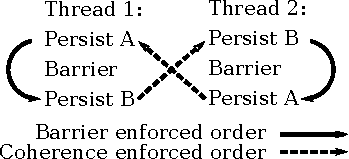
\includegraphics[width=.45\linewidth]{Persistency/cycle.pdf}
  \caption{\textbf{Cache Coherence Ordered Persists.} Thread 1's store visibility reorders while still attempting to enforce persist order.  The resulting persist order cycle is resolved by violating cache coherence persist order or by preventing stores from reordering across persist barriers.}
  \label{fig::Cycle}
\end{figure}


The example in Figure~\ref{fig::Cycle} demonstrates that it is not possible to simultaneously (1) allow store visibility to reorder across persist barriers, (2) enforce persist barriers, and (3) enforce persist order to a single address according to the order cache coherence observes those stores.
The example considers two distinct persistent objects, A and B.
Threads 1 and 2 persist to these objects in different program orders.
Thread 1's execution reorders the visibility of stores, while Thread 2 executes its stores in program order.
Note that the persist barrier implies that thread 1's persist to B occurs after its persist to A, but the values produced by these operations may become visible to other processors out of program order.

Figure~\ref{fig::Cycle} additionally annotates the persist order constraints (happens-before relationships) due to persist barriers and cache coherence store order.
As shown, these constraints form a cycle and hence cannot be enforced.
The cycle can be resolved by either coupling persist and store barriers---every persist barrier also prevents store visibility from reordering---or relaxing cache coherence persist order and providing additional mechanisms to order persists across threads.
It remains unclear how to best solve this dilemma.

%\textbf{Consistency and persistency interaction.}
%The consistency model and persistency model define separate memory orders (volatile memory order and persistent memory order) each containing the same memory events but distinct ordering constraints.
%The ordering constraint sets may be identical, as in strict persistency.
%Typical uses of relaxed persistency result in persistent memory order's constraint set being a subset of volatile memory order's constraint set.
%However, it is possible for persisent memory order to introduce ordering constraints not found in volatile memory order (e.g., a persist barrier that does not enforce store visibility order).
%Taken to an extreme, neither set of ordering constraints is a subset of the other.
%
%Additionally, persistent memory execution affects volatile memory execution.
%For example, once a cache line is evicted, the next load will retrieve the value stored by the most recent \emph{persist,} defined by persistent memory order, not volatile memory order.
%Therefore, any ordering constraints between stores/persists to the same address in volatile memory order must also be present in persistent memory order.
%If this cannot be enforced (e.g., additional constraints on persistent memory order introduce a cycle) the consistency and persistency models must be modified or behavior declared undefined (and thus the model specifies that it is up to the programmer to avoid such situations and how to do so).
%

\textbf{Store atomicity.}
Cache coherence provides \emph{store atomicity} for memory consistency models and their resulting memory orders \cite{Adve96}.
Store atomicity requires that stores become visible in their entirety (no partial stores) and that stores are atomically visible to all processors, and thus stores to each address are serializable.
Store atomicity is violated when a store is visible to only a subset of processors (although many memory systems allow store buffering and forwarding within the same processor without violating store atomicity).
Similar principles apply to memory persistency.

I define a memory persistency model to be \emph{persist-atomic} if persists to the same address are serializable.
Equivalently, a model is persist-atomic if recovery establishes a single unique value for each address in the persistent address space.
While persist atomicity requires that persists of a certain size occur atomically, persist atomicity additionally places constraints on the order of persists.
Persist atomicity is violated when processors recover different values for the same address (e.g., processors recover using persistent per-processors logs---similar behavior in distributed caches violates store atomicity).

Store and persist atomicity are useful features for defining intuitive consistency and persistency models.
However, it is entirely possible for a memory model to exhibit both store and persist atomicity, but for the order of stores and persists to deviate.
In such cases persists to the same address are reordered relative to their underlying stores but still retain some total order.
I additionally define \emph{strong persist atomicity} to describe memory models that provide both store and persist atomicity and where the order of stores to each address agrees with the order of persists.
All persistency models discussed in the remainder of this study provide strong persist atomicity.

\section{Conclusion}
\label{sec:Persistency:Conclusion}

Existing memory systems lack mechanisms to describe and enforce the order of persists.
I introduce memory persistency to explore the design space of interfaces and semantics for persistent memory.
Memory persistency builds on memory consistency to determine the values for and order of persist operations.
Memory persistency may be strict, relying on the consistency model to provide both thread and persist synchronization, or relaxed, decoupling thread synchronization from persist order and requiring additional persist barriers.
The next chapter introduces three persistency models and details their expected performance using a thread-safe persistent queue.


 \chapter{Memory Persistency Models}
 \label{chap:PersistencyModels}
 This chapter provides examples of memory persistency models and data structures using the memory persistency framework defined in the previous chapter.
I first introduce a concurrent, persistent queue, outlining several design choices and reasoning about persist performance.
I then define specific memory persistency models under sequential consistency (SC), demonstrating their use with the persistent queue.
The final chapter of this dissertation evaluates these persistency models using the persistent queue.

\section{Persistent Queue}
\label{sec:PersistencyModels:Queue}

To understand and evaluate persistency models I first introduce a motivating benchmark: a thread-safe persistent queue.
Several workloads require high-performance persistent queues, such as write ahead logs (WAL) in databases and journaled file systems.
Previous work investigated the design of an NVRAM log assuming byte-addressable NVRAM with a persist barrier \cite{FangHsiao11}.
I extend this work, outlining three queue designs with several persistency models.

Fundamentally, a persistent queue inserts and removes entries while maintaining their order.
The queue must recover after failure, preserving proper entry values and order.

My goals in designing a persistent queue are to (1) maximize the instruction execution rate, including multi-thread throughput, (2) improve the persist concurrency of insert operations through greater thread concurrency, and (3) further improve persist concurrency using relaxed persistency.
All designs are concurrent (thread-safe) but allow varying degrees of persist concurrency.
Additionally, the three designs are fashioned as circular buffers, containing a data segment and head and tail pointers.
Psuedo-code for the three designs is shown in Figure~\ref{Alg::Queue}.
I outline their execution, recovery, and the minimal necessary persist dependences.

\begin{figure}

%\begin{algorithm}
  \caption{\textbf{Psuedo-code for insert operations.}  I include the annotations required by relaxed persistency models, discussed in Section~\ref{sec:PersistencyModels:Models}.  $PersistBarrier$ applies to epoch persistency and strand persistency, $NewStrand$ applies only to strand persistency.}
  \label{Alg::Queue}
  \begin{algorithmic}[1]
  \Require $head$ is a persistent pointer, $data$ a persistent array.
  \State $sl \gets$ \Call{sizeof}{length}
  \Function{InsertCWL}{$length$, $entry$}
    \State \Call{lock}{$queueLock$}
    \State \Call{NewStrand}{}
    \State \Call{copy}{$data[head]$, ($length$, $entry$), $length+sl$}
    \State \Call{PersistBarrier}{}
    \State $head \gets head+length+sl$
    \State \Call{unlock}{$queueLock$}
  \EndFunction
  \State
  \Function{Insert2LC}{$length$, $entry$}
    \State \Call{lock}{$reserveLock$}
    \State $start \gets headV;$ $headV \gets headV+length+sl$
    \State $node \gets insertList$.\Call{append}{$headV$}
    \State \Call{unlock}{$reserveLock$}
    \State \Call{NewStrand}{}
    \State \Call{copy}{$data[head]$, ($length$, $entry$), $length+sl$}
    \State \Call{lock}{$updateLock$}
    \State ($oldest$, $newHead$) $\gets insertList$.\Call{remove}{$node$}
    \State \Call{unlock}{$updateLock$}
    \If{$oldest$}
      \State \Call{PersistBarrier}{}
      \State $head \gets newHead$
    \EndIf
    \State $unlock(reserveLock)$
  \EndFunction
  \State
  \Function{InsertQH}{$length$, $entry$}
    \State \Call{lock}{$queueLock$}
    \State \Call{NewStrand}{}
    \State $start \gets head$; $endPos \gets start+length+sl$ %\Comment{marks $endBit$}
    \State $data[start] \gets length$; $data[endPos] \gets 0$
    \State \Call{PersistBarrier}{}
    \State $head \gets head+length+sl+1$
    \State \Call{unlock}{$queueLock$}
    \State \Call{copy}{$data[start+sl]$, $entry$, $length$}
    \State \Call{PersistBarrier}{}
    \State $data[endPos] \gets 1$
  \EndFunction
  \end{algorithmic}
%\end{algorithm}

\end{figure}


The first design, \emph{Copy While Locked} (CWL), serializes insert operations with a lock, first persisting each entry's length and data to the queue's data segment, then persisting the new head pointer.
As a result, persists from subsequent insert operations, even if they occur on separate threads, are ordered by lock accesses.
If the systems fails before the persist to the head pointer in line 6, the entry is ignored and the insert has failed.

I improve persist concurrency in the second design, \emph{Two-Lock Concurrent} (2LC), by using two different locks to reserve data segment space and persist to the head pointer, respectively.
Neither lock is held while entry data persists to the data segment, allowing concurrent persists from different threads.
Additionally, a volatile \emph{insert list} is maintained to detect when insert operations complete out of order and prevent holes in the queue.
The double-checked locking pattern prevents data races while updating the insert queue.
\emph{Two-Lock Concurrent} employs the same recovery as \emph{Copy While Locked}---an entry is not valid and recoverable until the head pointer encompasses the associated portion of the data segment.

\begin{figure}
  \centering
  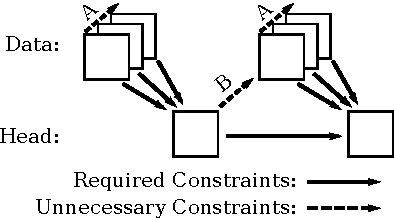
\includegraphics[width=.55\linewidth]{PersistencyModels/CWL_2LC_dependences.pdf}
  \caption{\textbf{Queue Persist Dependences.} Persist ordering dependences for \emph{Copy While Locked} and \emph{Two-Lock Concurrent}.  Constraints necessary for proper recovery shown as solid arrows; unnecessary constraints incurred by strict persistence appear as dashed arrows and are labelled as A (removed with epoch persistency) and B (further removed by strand persistency).}
  \label{fig::CWL_dependences}
\end{figure}


Both queue designs use the persistency model to prevent persists to the head pointer from occurring before persists to the data segment.
Figure~\ref{Alg::Queue} includes barriers for two different persistency models (described later in Section~\ref{sec:PersistencyModels:Models}).
Additionally, persist dependences (and unnecessary constraints introduced by strict persistency models) are shown in Figure~\ref{fig::CWL_dependences}.
Recovery requires that persists to the head pointer are ordered after persists to the data segment from the same insert operation and persists to the head pointer occur in insert-order to prevent holes in the queue (persists to the head pointer may coalesce so long as no ordering constraint is violated).
All other persists within the same insert operation and between operations may occur concurrently without compromising recovery correctness.

While not necessary for correct recovery, these persist dependences are difficult to describe minimally; ordering mechanisms often introduce unnecessary persist constraints (dashed lines in the Figure).
Persistency models that enforce program order of persists in each thread must serialize persists for the data of each entry to the data segment (when the entire entry cannot be persisted atomically), shown as ``A" in the Figure.
Additionally, persists to the data segment may be ordered after a previous insert's persist to the head pointer, denoted as ``B" in the Figure.

The previous designs trade off concurrency and complexity.
\emph{Copy While Locked}, while simple, serializes persists between insert operations.
On the other hand, \emph{Two-Lock Concurrent} allows greater concurrency, but requires two locks be acquired per insert and a volatile \emph{insert list} be maintained.
I consider a third design, \emph{Queue Holes}, that provides both improved persist concurrency and a high execution rate (first introduced in \cite{FangHsiao11}).

\begin{figure}
  \centering
  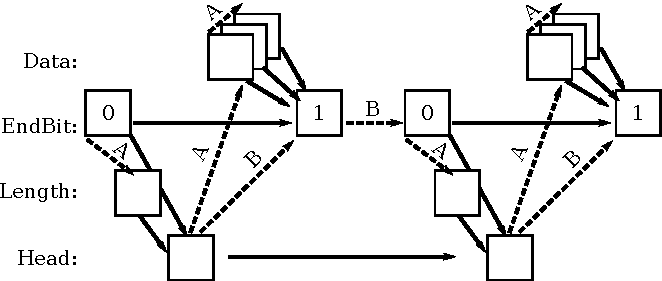
\includegraphics[width=\linewidth]{PersistencyModels/holes_dependences.pdf}
  \caption{\textbf{\emph{Queue Holes} Dependences.} The head pointer may not persist before \emph{endBit} and length; final \emph{endBit} may not persist until the entry persists to the data segment.  Strict persistency introduces several unnecessary constraints.}
  \label{fig::holes_dependences}
\end{figure}


\emph{Queue Holes} prepends each queue entry with its length and appends the entry with an endBit.
A single lock is held while reserving queue space and updating the head pointer, but is released prior to persisting the entry into the data segment.
An entry is recovered after failure if the entry is located within the region indicated by the head pointer (as in CWL and 2LC) and the entry's endBit is set.
The minimal set of persist dependences necessary for correct recovery are shown in Figure~\ref{fig::holes_dependences}.
The length and cleared endBit persist before the head pointer; the data segment persists before setting the endBit; and persists to the same address occur in the order observed by cache coherence (endBits and the head pointer).
An inserted entry is recoverable only after the persist at line 37 completes, even though the head pointer is persisted earlier at line 33.

As with the other queue designs many unnecessary persist constraints may be introduced by strict persistency models, shown as dashed lines in Figure~\ref{fig::holes_dependences}.
Many constraints are introduced by persistency models that enforce the program order of persists, labeled ``A."
Additional constraints may be introduced between persists within an insert operation or across insert operations, labeled ``B."

\section{Memory Persistency Models}
\label{sec:PersistencyModels:Models}

Section~\ref{sec:Persistency:Persistency} outlined potential classes of persistency models.
I now introduce several specific persistency models to be evaluated in the next chapter.
All models assume SC as the underlying memory consistency model, and successively relax persistency to introduce specific optimizations.
For each model I discuss its motivation, give a definition, describe necessary annotations for and performance of the persistent queues, and offer possible implementations.

\subsection{Strict Persistency}
\label{section:PersistencyModels:Strict}

\textbf{Motivation.}
The first persistency model is Strict Persistency, as discussed in Section~\ref{sec:Persistency:Persistency}.
Strict persistency simplifies reasoning about persist ordering by coupling persist dependences to the memory consistency model.
No additional persist barriers are required, easing the burden on the programmer.
While strict persistency provides an intuitive first model, under SC, it imposes persist ordering constraints that unnecessarily limit persist concurrency for many data structures, and requires programmers to resort to multi-threading to obtain concurrency.

\textbf{Definition.}
Under strict persistency, persist order observes all happens-before relations implied by execution's dynamic order of memory operations as viewed by the recovery observer.
Thus, all persists are ordered with respect to the program order of the issuing thread.
Note that, like store operations, persists from different threads that are unordered by happens-before (i.e., the recovery observer cannot distinguish which is first) are concurrent.

\textbf{Persist Performance.}
Strict persistency under SC introduces many unnecessary persist dependences.
Consequently, strict persistency must rely entirely on thread concurrency to enable concurrent persists.
Figures~\ref{fig::CWL_dependences} and~\ref{fig::holes_dependences} illustrate these unnecessary dependences and their causes.
Lacking mechanisms to relax persist ordering, strict persistency under SC introduces all the shown dependences (dashed lines).

These dependences are introduced because persists occur in program order under SC.
This persistency model lacks the ability to declare two persists from the same thread to be concurrent.
However, persist concurrency may be created by using multiple threads to concurrently insert into the queue.
\emph{Two-Lock Concurrent} and \emph{Queue Holes} each allow concurrent inserts, and thus persists from different threads into the data segment are concurrent---The dashed line labeled ``B" in Figure~\ref{fig::CWL_dependences} no longer implies a constraint.

\textbf{Implementation.}
A straight-forward implementation of strict persistency stalls issue of subsequent memory accesses until a store and its corresponding persist both complete.
Conventional speculation mechanisms may allow loads to speculatively reorder with respect to persistent stores \cite{Gharachorloo91}.
Buffered strict persistency can be implemented by serializing persists to a single, totally ordered queue in front of persistent memory (e.g., in a bus-based multiprocessor, persists can be queued after they are serialized by the bus).
Delays still occur when buffers fill, to drain the queue at persist sync instructions, or under contention to the persist queue.

More advanced implementations might consider distributed queues (i.e., one queue per thread/core) or extensions to the existing cache system.
Mechanisms must be introduced to ensure that persists of each thread occur in program order and that persists are ordered by conflicting accesses from different threads, but persists from several threads may occur concurrently (they are not serialized) while persists buffer and execution proceeds ahead of persistent state.
Under the definition of SC such implementations must detect load-before-store races between threads, ordering persists prior to the load (on the first thread) before persists after the store (on the second thread).
A single store may introduce persist ordering constraints with many threads, each having loaded data from the store's address.
It is unclear how to design a system that satisfies these constraints without frequent delays.

While insufficient for SC, TSO might be implemented by recording a ``persist counter" and thread in each cache line.
Each time a thread persists it increments its persist counter, and each store (both volatile stores and persists) writes the thread and persist counter into the cache line.
Persists drain in program order by maintaining a persist queue per thread/core.
Persist order between threads is enforced at each load and store by observing the previously recorded thread and counter in the operation's cache line---all subsequent stores from the executing thread must occur after the last persist to the cache line.
These inter-thread persist constraints may be recorded in threads' queues or by delaying immediately until the other thread's queue drains.
Such a system resembles BPFS (discussed next in Section~\ref{section:PersistencyModels:PersistEpochs} and later in Section~\ref{sec:PersistencyModels:RelatedWork}) where each persist occurs in its own epoch \cite{ConditNightingale09}.

Strict persistency under SC may also be implemented using in-hardware NVRAM logs or copy-on-write and indirection to give the appearance of SC while persists occur concurrently.
Hardware must ensure both that persists do not occur out of program order for any thread and that conflicting accesses properly enforce persist order across threads.
An intriguing possibility would be to leverage existing hardware transactional memories (HTM), partitioning program execution into transactions that enforce atomicity, isolation, and durability---resembling BulkSC with durable transactions \cite{CezeTuck07}.
Transactions must be long enough to minimize transaction overhead (including persist barriers for each durable transaction) and improve persist concurrency (by placing many persists in the same transaction), but short enough to bound resources necessary for atomic transactions (such as a log) and to minimize forward progress lost when a transaction aborts.
%Additionally, transactions may buffer persists so long as transactions become visible to recovery in their proper order.
%I leave it to future work to investigate how to coalesce persists between durable transactions.

\subsection{Epoch Persistency}
\label{section:PersistencyModels:PersistEpochs}

\textbf{Motivation.}
Strict persistency under SC introduces many persist dependences unnecessary for correct recovery.
The most common unnecessary persist dependence occurs due to the program-order constraint of SC.
Programs frequently persist to large, contiguous regions of memory that logically represents a single object, but which cannot occur atomically (due to their size).
Under strict persistency, the persists serialize.
I remove the program-order-implied persist order constraint with \emph{epoch persistency}, allowing consecutive persists from the same thread to reorder and persist in parallel.
Doing so, however, requires annotation by the programmer in the form of persist barriers to divide execution into epochs when ordering is required by the recovery algorithm.
Epoch persistency additionally allows persists to addresses protected by a lock to reorder with respect to the lock operations (e.g., avoid delaying the lock release while the persist completes); my queue implementations leverage this optimization opportunity.

\textbf{Definition.}
Epoch persistency defines a new \emph{persistent memory order} in addition to execution's existing memory order (referred to as the \emph{volatile memory order}).
Persistent memory order contains a subset of constraints from the volatile memory order.
Any pair of persists ordered in the persistent memory order may not be observed out of that order with respect to the recovery observer.

Volatile memory order satisfies SC.
Each thread's execution is additionally separated into \emph{persist epochs} by persist barrier instructions.
Epoch persistency provides several rules to inherit memory order constraints from the volatile memory order: (1) any two memory accesses on the same thread and separated by a persist barrier are ordered, (2) any two memory accesses (from the same or different threads) that conflict (they are to the same or overlapping addresses and at least one is a store/persist) assume the order observed from volatile memory order (enforced via cache coherence), and (3) eight-byte persists are atomic with respect to the recovery observer and failure.
This last rule is relaxed in my evaluation, requiring only that eight-byte \emph{aligned} persists be atomic.

Persist barriers enforce that no persist after the barrier may occur before any persist before the barrier.
Persists within each epoch (not separated by a barrier) are concurrent and may reorder or occur in parallel.
Additional complexity arises in reasoning about persist ordering across threads. 
I define a \emph{persist epoch race} as persist epochs from two or more threads that include memory accesses (to volatile or persistent memory) that race, including synchronization races, and at least two of the epochs include persist operations. 
In the presence of a persist epoch race, rules (1) and (2) order accesses prior to the epoch of the earlier access in the race before accesses following the epoch of the later access in the race.
Additionally, conflicting accesses are themselves ordered according to the volatile memory order.
Consequently, two persists to the same address are always ordered even if they occur in racing epochs.

\textbf{Discussion.}
Epoch persistency provides an intuitive mechanism to guarantee proper recovery as it is impossible at recovery to observe a persist from after a barrier while failing to observe a persist from before the same barrier.
However, many persists (those within the same epoch) are free to occur in parallel, improving persist concurrency.

As noted in the definition, reasoning about persist order across threads can be challenging.
Synchronization operations within persist epochs impose ordering across the store and load operations (due to SC memory ordering), but do not order corresponding persist operations.
Hence, persist operations correctly synchronized under SC by volatile locks may nevertheless result in astonishing persist ordering.
A simple (yet conservative) way to avoid persist epoch races is to place persist barriers before and after all lock acquires and releases, and to only place locks in the volatile address space.
The persist behavior of strict persistency can be achieved by preceding and following all persists with a persist barrier.

Persist epoch races may be intentionally introduced to increase persist concurrency; I discuss such an optimization below.
Enforcing persist order between threads with volatile locks requires that the persists be synchronized outside of the epochs in which the persists occur.
However, synchronization through persistent memory is possible.
Since persists to the same address must follow the order observed by cache coherence, even if they occur in epochs that race, the outcome of persist synchronization is well defined.
Hence, atomic read-modify-write operations to persistent memory addresses provide the expected behavior.

\textbf{Persist ordering example.}
\begin{figure}
  \centering
  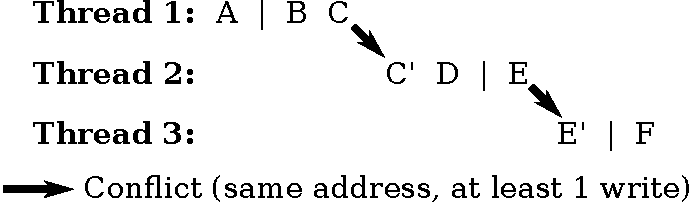
\includegraphics[width=.55\linewidth]{PersistencyModels/propagation.pdf}
  \caption{\textbf{Epoch persistency persist order.} Persistent memory order is enforced through persist barriers (shown as `` $\vert$ ") and access conflicts.  Access A is ordered by transitivity before access F.  If these accesses are persists they may not be reordered with respect to the recovery observer.  This order is enforced even if accesses are to the volatile address space.  Access B is concurrent with all shown accesses from threads 2 and 3, while access D is concurrent with accesses from thread 1.}
  \label{fig::EpochPersistencyPropagation}
\end{figure}

Figure~\ref{fig::EpochPersistencyPropagation} demonstrates a sample memory execution and the resulting persistent memory order.
Capital letters denote memory accesses (loads, stores, and persists), accesses labeled by the same letter are to the same address.
`` $\vert$ " implies a persist barrier.
Arrows show access conflicts and the order that the conflict is observed in volatile memory order.

According to rule (1) of epoch persistency all accesses on the same thread are ordered if separated by a persist barrier (A before B and C; C' and D before E; and E' before F).
By rule (2) all conflicts are ordered according to volatile memory order (C before C'; E before E').
Transitivity of these rules additionally orders accesses (A before C', E, E', and F; C before E, E', and F; C' and D before E' and F; and E before F).
Notably, B is unordered with all shown accesses by threads 2 and 3, and D is unordered with accesses by thread 1 (such accesses are concurrent).
Any accesses that are persists may not be observed out of this order by the recovery observer (e.g., a persist to F may not be observed while a persist to A is not).

This order is enforced on conflicts (between C and C'; E and E') to both volatile and persistent address spaces and as long as one of the accesses is a store or persist.
This includes the case where the first access is a load and the second a store/persist.
Providing an implementation to enforce this constraint remains a challenge, as persists must complete before a subsequent load executes or all load-store conflicts must be detected and enforced at some later time.

The resulting persist order resembles RMO \cite{SPARCv9} with (at least) one important difference: memory order constraints introduced due to control and register data dependencies do not impose a persistent memory order constraint in epoch persistency.
For example, consider that access C is a persist, C' a load, and D a persist whose value depends on C'.
According to RMO such a register dependence initiated by a load introduces a (volatile) memory order constraint.
Strict persistency under RMO would now allow persist D to be observed without also observing persist C.
Epoch persistency, on the other hand, allows such behavior, violating RMO.
In general persistent memory order need not order accesses that contain a register dependence, but this may produce unintuitive or unintended behavior.

\textbf{BPFS.}
My definition of epoch persistency is inspired by the programming model and hardware extensions for caching persistent memory proposed for the Byte-addressable Persistent File System (BPFS) \cite{ConditNightingale09}.
However, I introduce several subtle differences that I believe make epoch persistency a more intuitive model.
My definition considers all memory accesses when determining persist ordering among threads, whereas the BPFS memory system orders persists only when conflicts occur to the persistent address space.
While the BPFS file system implementation avoids persist epoch races, it is not clear that the burden falls to the programmer to avoid such accesses or what persist behavior results when such races occur (I believe the BPFS authors' intent was to prohibit programs containing such races---the cache implementation deadlocks under persist epoch races containing circular persist dependences).  
Furthermore, BPFS detects conflicts to the persistent address space by recording the last thread and epoch to persist to each cache line; the next thread to access that line will detect the conflict.
Such an implementation, however, cannot detect conflicts where the first access is a load and the second a store.
While occasionally unintuitive, such behavior rarely results in unintended behavior and greatly simplifies the memory system.
Existing memory consistency models similarly order accesses, including TSO \cite{SPARCv9}).

\textbf{Persist Performance.}
Epoch persistency removes all unnecessary persist dependences that result from strict persistency's program order constraint.
All versions of the persistent queue benefit from allowing persist entries to persist to the data segment concurrently.
Additionally, \emph{Queue Holes} allows entry length and \emph{endBit} to persist concurrently (although both are ordered with respect to the subsequent persist of the head pointer).
Finally, many persist constraints between threads are removed by intentionally allowing persist epoch races.
Lock operations occur in the same epoch as the first persists of the insert operation, while unlock operations occur in the same epoch as the last persists; persists from the last epoch of an insert and the first epoch of the subsequent insert are concurrent.
As a result, persists protected by a lock now occur concurrently.
\emph{Copy While Locked} and \emph{Queue Holes} retain recovery correctness by still ordering all persists to the head marker (persists occur according to cache coherence order).

Figure~\ref{Alg::Queue} demonstrates how to use epoch persistency's barriers (shown in the code as $PersistBarrier$) within each queue design.
The constraints in Figures~\ref{fig::CWL_dependences} and~\ref{fig::holes_dependences} annotated with ``A" are removed under epoch persistency relative to strict persistency.

\textbf{Implementation.}
BPFS \cite{ConditNightingale09} outlines cache extensions that provide a persistency model similar to persist epochs, assuming the TSO consistency model.
Modifications must be made to detect load-before-store conflicts (and thus enforce SC rather than TSO ordering) and track conflicts to volatile memory addresses as well as persistent memory addresses; detecting load-before-store conflicts and enforcing persist order without frequent delays remains an open problem.
Instead of delaying execution to enforce persist ordering among threads, optimized implementations avoid stalling execution by buffering persists while recording and subsequently enforcing dependences among them, allowing persists to occur asynchronously despite access conflicts.

More advanced techniques might rely on hardware NVRAM logging and hardware transactional memory, partitioning program execution into transactions as discussed above for strict persistency.
Under epoch persistency any transaction that contains only a single epoch need not persist atomically, and therefore logging is unnecessary (persist order must still be enforced between transactions).
Persist barriers may be used as hints to establish transaction boundaries and minimize durable transaction logging.

\subsection{Strand Persistency}
\label{section:PersistencyModels:PersistStrands}

\textbf{Motivation.}
Epoch persistency relaxes persist dependences within and across threads.
However, only consecutive persists within a thread may be labeled as concurrent.
Likewise, persists from different threads are only concurrent if their epochs race or if they are not synchronized.
Many persists within and across threads may still correctly be made concurrent even if they do not fit these patterns.
I introduce \emph{strand persistency}, a new model to minimally annotate persist dependences.

\textbf{Definition.}
A strand is an interval of memory execution from a single thread.
Strands are separated via \emph{strand barriers}; each strand barrier begins a new strand.
The strand barrier clears all previously observed persist dependences from the executing thread.
Within each strand new and observed persists are ordered using persist barriers according to the epoch persistency model.
Rule (1) of epoch persistency may be modified to read: any two memory accesses on the same \emph{strand} separated by a persist barrier assume the order observed from volatile memory order (accesses from different strands never assume a program order constraint, and will only be ordered through conflicts or ordering constraints with accesses in the same strand).
Rules (2) and (3) of epoch persistency apply without modification.

\textbf{Discussion.}
There are no implicit persist ordering constraints across strands for persists to different addresses on the same thread of execution.
Ordering constraints arise only for persists to the same address as implied by cache coherence.
Hence, persists on a new strand may occur as early as possible and overlap with all preceding persists.
Strand persistency allows programmers to indicate that logical tasks on the same thread are independent from the perspective of persistency.
To enforce necessary ordering, a persist strand begins by reading any memory locations after which new persists must be ordered.
These reads introduce an ordering dependency due to cache coherence, which can then be enforced with a subsequent persist barrier.
This programming interface allows ordering constraints to be specified at the granularity of individual addresses; the minimal set of persist dependences is achieved by placing each persist in its own strand, loading all addresses the persist must depend on, inserting a persist barrier, and then executing the persist.

The performance of epoch persistency is achieved by using a single persist strand on each thread (strand persistency is equivalent to epoch persistency under such conditions).
While I enforce persist order within strands according to epoch persistency, other persistency models may be used (e.g., strict persistency/SC orders persists within strands but new strands clear previously observed dependences).

While intended for persistency, strand persistency additionally functions as a consistency model (\emph{strand consistency}).
Strand consistency requires full memory barriers in lieu of persist barriers; loads and stores may not reorder across memory barriers.
Additionally, the execution of loads and stores may not reorder across strand barriers for the purpose of observing memory dependences between strands on the same thread, but loads and stores from different strands that do not interact may reorder with respect to other processors and threads.
Dependences propagate through memory execution and cache coherence, with strands from the same thread being concurrent if they do not share conflicts through memory (i.e., the visibility of loads and stores from different strands may reorder).
Recent trends suggest that such a relaxed consistency model is unnecessary for typical memory architectures as memory systems have tended towards stricter models with improved performance.

\textbf{Persist Performance.}
The persistent queue implementations place each insert task in a separate persist strand.
The result is that all unnecessary persist constraints are removed, including constraints between inserts from the same thread.
Figure~\ref{Alg::Queue} includes the necessary strand persistency annotations ($NewStrand$ and $PersistBarrier$).
All unnecessary constraints from Figures~\ref{fig::CWL_dependences} and~\ref{fig::holes_dependences} are removed; those removed in moving from epoch persistency to strand persistency are labeled ``B."
The required persist dependences (and only those required for correct recovery) remain, maximizing persist concurrency.

\textbf{Implementation.}
Strand persistency builds on the hardware requirements to track persist dependencies as in epoch persistency, but further requires mechanisms to separate tracking of dependencies for different strands.
In addition to tracking the last thread to access each persistent location, the strand within the thread must also be tracked.
Unordered persists on different strands can traverse separate queues (e.g., on separate virtual channels) throughout the persistent memory system.
Strand persistency gives enormous implementation latitude and designing efficient hardware to track and observe only the minimal ordering requirements remains an open research challenge.
In this work, I focus on demonstrating the potential performance that the model allows.

\section{Related Work}
\label{sec:PersistencyModels:RelatedWork}

Durable storage has long been used to recover data after failures.
All systems that use durable storage must specify and honor dependencies between the operations that update that storage.
For example, file systems must constrain the order of disk operations to metadata to preserve a consistent file system image~\cite{Ganger00,Chidambaram13}, and databases must obey the order of durable storage updates specified in write-ahead logging~\cite{MohanHaderle92}.

Specifying and honoring these dependencies becomes harder when the interface to durable storage are loads and stores to a persistent address space.
Store instructions to an address space are more frequent and fine grained than update operations when using a block-based interface to durable storage (such as a file system).
In addition, CPU caches interpose on store instructions, which leads to the interaction of persistency and cache consistency discussed in this dissertation.

Recent developments in nonvolatile memory technologies have spurred research on how to use these new technologies.
Some research projects keep the traditional block-based interface to durable storage and devise ways to accelerate this interface~\cite{CaulfieldDe10}.
Other projects provide a memory-based interface to durable storage~\cite{CoburnCaulfield11}.
My approach follows the path of providing a memory-based interface to durable storage, arguing that the high speed and fine-grained access of new nonvolatile memories provides a natural fit with native memory instructions.

Combining a memory interface to durable storage with multiprocessors adds concurrency control issues to those of durability.
Transactions are a common and powerful paradigm for handling both concurrency control and durability, so many authors have proposed layering transactions on top of nonvolatile memory~\cite{Lowell97,CoburnCaulfield11,VolosTack11,Coburn13}.
Similarly, a recent paper proposes to couple concurrency control with recovery management by committing execution to durable storage at the granularity of the outermost critical section~\cite{Chakrabarti13}.

While transactions and critical sections are powerful mechanisms for concurrency control, many programs use other mechanisms besides these, such as conditional waits.
Because of this diversity of concurrency control, I believe it is useful to treat the issues of consistency and persistency separately.
Just as much work has been done to create a framework of memory consistency models~\cite{Adve96}, I seek to begin a framework on memory persistency models.

\textbf{Kiln.}
Zhao \emph{et al.} recently proposed Kiln, a persistent system using multi-versioning in a persistent cache to provide durable transactions \cite{ZhaoLi13}.
A key feature of this system is that persistence control and thread synchronization are de-coupled; persistent transactions do not ensure isolated transactions (I believe it is implied that additional synchronization must already ensure that transactions are isolated).
Several persistent transactions may occur within a single critical section without the thread synchronization overheads of isolated multi-thread transactions.

In my work I investigate additional interactions between thread communication and persist ordering.
Kiln provides no mechanism to allow concurrent persists between interacting threads as I do with epoch persistency and strand persistency.
Zhao introduces ordered and unordered transactions, but it is unclear if ordered transactions are totally ordered between all threads or interact with thread synchronization to establish order, and how to enforce any order with unordered transactions (completely unordered transactions do not provide functionality for useful recovery).
Finally, as with racing persist epochs, durable transactions that race break transaction atomicity; persists to cache lines that contain conflicting writes from two transactions may reach NVRAM (and be visible at recovery) before or after the transactions commit.
A precise persistency model must specify how to avoid such behavior or what intended behavior results from persistent transaction races.

\textbf{BPFS.}
The techniques most closely related to those proposed in this dissertation are the primitives for describing persist dependencies in the Byte-Addressable Persistent File System (BPFS)~\cite{ConditNightingale09}.
Condit \emph{et al.} introduce \emph{persist barriers}, similar to existing memory barriers, that constrain the order of writes to the persistent address space.
Any two persists separated by a barrier must occur in program order, but persists within the same epoch (interval of execution separated by barriers) are concurrent.
Additionally, Condit assumes that NVRAM allows eight byte atomic writes, allowing many updates to write atomically in-place without additional recovery mechanisms.
Finally, the proposed cache implementation allows volatile execution of each thread to proceed ahead of the persistent state, although sharing persistent data between threads causes processors to stall.
I assume similar mechanisms.

I view BPFS as a single point in the memory persistency design space.
While similar to my epoch persistency design, there are subtle, yet important differences, described in Section~\ref{section:PersistencyModels:PersistEpochs}.
I highlight complications with the BPFS programming model, specifically persist epoch races.
Epochs that race and form a cycle may cause the BPFS system to deadlock.
This problem remains when the access cycle occurs at cache line granularity (false sharing), even if true races do not occur.
An important aspect of memory persistency is to precisely define allowable behavior under such scenarios.
I investigate the more-general design space of memory persistency and its interactions with memory consistency.

\textbf{Alternatives to persistent storage.}
Recent work (e.g., H-Store \cite{StonebrakerMadden07}) suggests highly available systems as an outright replacement for durability.
Additionally, battery-backed memory and storage obviate the need for memory persistency, allowing more expensive persist synchronization only when necessary (e.g., Whole-System Persistence \cite{NarayananHodson12}).
I argue that computers and storage systems will always fail, and durability remains a requirement for many applications.

More importantly, highly available systems and battery-backed storage are not universally available.
Mobile devices, for example, must rely on persistent storage for data recovery.
Devices in the "Internet of Things" will require high performance while recovering after failure.
Any device expected to fail frequently (due to low power operation or unreliable power sources) can use memory persistency alongside NVRAM to improve performance while retaining data integrity.

\section{Conclusion}
\label{sec:PersistencyModels:Conclusion}

Relaxed persistency offers new tools to enforce recovery correctness while minimizing delays due to persists.
In the next chapter I use these queue designs and persistency models to quantitatively evaluate the opportunity relaxed persistency holds to improve performance with NVRAM.


 \chapter{An Evaluation of Memory Persistency}
 \label{chap:PersistencyEval}
 The previous two chapters described a recoverable persistent queue data structure as well as three memory persistency models.
This chapter uses the queue and models to motivate the need for relaxed memory persistency models.
First, I describe the methodology used for this evaluation.

\section{Methodology}
\label{sec:PersistencyEval:Methodology}

To evaluate persistent queue designs and persistency models I measure instruction execution rate on a real server and persist concurrency via memory traces.
All experiments run the queue benchmarks optimized for volatile performance.
Memory padding is inserted to objects and queue inserts to provide 64-byte alignment to prevent false sharing.
%All threads are constrained to a single socket using the Linux \emph{taskset} utility.
Critical sections are implemented using MCS locks \cite{Mellor-Crummey91}, a high-throughput queue based lock.
Experiments insert 100-byte queue entries.
%Once the queue fills a thread flash-clears the queue by copying the entire valid portion of the data segment at once and updating the circular buffer tail pointer, simulating an archive process.
%Archiving in this manner minimizes interference between archive threads and inserting threads that would otherwise increase lock contention increase persist ordering constrain critical path.
Instruction execution rate is measured as inserts per second while inserting 100,000,000 entries between all threads using an Intel Xeon E5645 processor (2.4GHz).
The remainder of this section describes how I measure persist concurrency for the queue benchmarks.

\textbf{Persist Ordering Constraint Critical Path.}
Instead of proposing specific hardware designs and using architectural simulation, I instead measure, via memory traces, the persist ordering constraint critical path.
The evaluation assumes a memory system with infinite bandwidth and memory banks (so bank conflicts never occur), but with finite persist latency.
Thus, persist throughput is limited by the longest chain (critical path) of persist ordering constraints observed by execution under different memory persistency models.
While real memory systems must necessarily delay elsewhere due to limited bandwidth, bank conflicts, and other memory-related delays incurred in the processor, measuring persist ordering constraint critical path offers an implementation-independent measure of persist concurrency.

%Measuring persist critical path still requires several assumptions about the memory system.
I measure persist critical path under the following assumptions.
Every persist to the persistent address space occurs in place (there is no hardware support for logging or indirection to allow concurrent persists).
I track persist dependences at variable granularity (e.g., eight-byte words or 64-byte cache lines).
Coarse-grained persist tracking is susceptible to false sharing, introducing unnecessary persist ordering constraints due to accesses to the same cache line but not to overlapping addresses.
I similarly track persist coalescing with variable granularity.
Every persist attempts to coalesce with the last persist to that address.
A persist successfully coalesces if the persist fits within an atomically persistable memory block and coalescing with the previous persist to the same block does not violate any persist order constraints.
%Both persist dependence tracking and coalescing occurs within aligned blocks of memory.
%Using these assumptions, we generate memory access traces and simulate persist timing to determine persist ordering constraint critical path.

\textbf{Memory Trace Generation.}
I use PIN to instrument the queue benchmarks and generate memory access traces \cite{LukCohn05}.
Tracing multi-threaded applications requires additional work to ensure analysis-atomicity---application instructions and corresponding instrumentation instructions must occur atomically, otherwise the traced memory order will not accurately reflect execution's memory order.
I provide analysis atomicity by creating a bank of locks and assigning every memory address (or block of addresses) to a lock.
Each instruction holds all locks corresponding to its memory operands while being traced.
%Locks are numbered and acquired in lock number-order to avoid deadlocks.
%In addition to tracing memory accesses, we instrument the queue benchmarks with region-of-interest markers, persist barriers, and persistent malloc/free to distinguish persistent and volatile address spaces.
%Each annotation is implemented as a standard function and instrumented in PIN.
In addition to tracing memory accesses, I instrument the queue benchmarks with persist barriers and persistent malloc/free to distinguish volatile and persistent address spaces.
My tracing infrastructure is publicly available \cite{AtomicMemoryTrace}.

Tracing memory accesses in such a way ensures that the trace accurately reflects the order of memory accesses from execution.
%However, as only one instruction from any thread can access each memory region at once, and instructions on each thread occur in program order, our trace is limited to SC.
As only one instruction from any thread can access each address at once, and instructions on each thread occur in program order, the trace observes SC.
Thus, all evaluated memory persistency models assume SC as the underlying consistency model.

\textbf{Performance Validation.}
It is important that tracing not heavily influence thread interleaving, which would affect persist concurrency.
I measure the distance of insert operations between successive inserts from the same thread.
I observe that the distribution of insert distance is the same when running each queue natively and with instrumentation enabled, suggesting that thread interleaving is not significantly affected.

\textbf{Persist Timing Simulation.}
%Using the memory trace we measure persist ordering constraint critical path as the time of the last persist from any thread.
Persist times are tracked per address (both persistent and volatile) as well as per thread according to the persistency model.
For example, under strict persistency each persist occurs after or coalesces with the most recent persists observed through (1) each load operand, (2) the last store to the address being overwritten, and (3) any persists observed by previous instructions on the same thread.
Persists' ability to coalesce is similarly propagated through memory and thread state to determine when coalescing will violate persist ordering constraints---a persist may coalesce if its most recent persist dependence (greatest timestamp) occurs to the same atomically persistable memory block and all other persist dependences are strictly older (timestamp strictly less).
Under such situations coalescing will not violate any of the earlier persist dependences.
The persistency models differ as to the events that propagate persist ordering constraints through memory and threads.

Next, I use this methodology to establish the need for relaxed persistency models, as well as measure their opportunity to accelerate recoverable systems.

\section{Evaluation}
\label{sec:PersistencyEval:Evaluation}

This section uses the previously described methodology to demonstrate that persist ordering constraints present a performance bottleneck under strict persistency.
However, relaxed persistency improves persist concurrency, removing stalls caused by persists.
I also show that relaxed persistency models are resilient to large persist latency, allowing maximum throughput as persist latency increases.
Finally, I consider the effects of larger atomic persists and coarse-grained persist dependence tracking. 

\subsection{Relaxed Persistency Performance}
\label{section:Evaluation:PersistencyPerformance}

NVRAM persists are only a concern if they slow down execution relative to non-recoverable systems.
If few enough persists occur, or those persists are sufficiently concurrent, performance remains bounded by the rate that instructions execute with few delays caused by persists.
To determine system performance, I assume that only one of the instruction execution rate and persist rate is the bottleneck: either the system executes at its instruction execution rate (measured on current hardware), or throughput is limited solely by persist rate (while observing persist dependencies and retaining recovery correctness).

\begin{table*}
  \centering
  \begin{tabular}{ l l l l l l l l l l }
    \hline
    Threads & \multicolumn{3}{c}{Copy While Locked} & \multicolumn{3}{c}{Two-Lock Concurrent} & \multicolumn{3}{c}{Queue Holes} \\
    & Strict & Epochs & Strands & Strict & Epochs & Strands & Strict & Epochs & Strands \\
    \hline \hline
    %1 & 0.03402668948225257 & 0.17329066524439704 & 12.395878787878786 & 0.07956161591630416 & 0.5569551810923878 & 28.931290043290044 & 0.03243921666510665 & 0.17329066524439704 & 13.36387317909169 \\
    %8 & 0.05787677206992028 & 3.167189491481337 & 21.084432900432898 & 0.4319337035691424 & 3.3529680365296803 & 21.615757575757577 & 0.2539605628870943 & 1.9442439473904665 & 19.535723905723902 \\
    1 & 0.034 & 0.17 & \textbf{12} & 0.080 & 0.56 & \textbf{29} & 0.032 & 0.17 & \textbf{13} \\
    8 & 0.058 & \textbf{3.2} & \textbf{21} & 0.43 & \textbf{3.4} & \textbf{22} & 0.25 & \textbf{1.9} & \textbf{20} \\
    \hline
  \end{tabular}
  \caption{
    \textbf{Relaxed Persistency Performance.}
    Persist-bound insert rate normalized to instruction execution rate assuming 500ns persist latency.
    System throughput is limited by the lower of persist and instruction rates---at greater than 1 (bold) instruction rate limits throughput; at lower than 1 execution is limited by the rate of persists.
    While strict persistency limits throughput, persist epochs maximizes performance for many threads and persist strands are necessary to maximize performance with one thread.
  }
  \label{table::RelaxedPerformance}
\end{table*}


Table~\ref{table::RelaxedPerformance} shows the achievable throughput for the queue benchmarks and persistency models for both one and eight threads assuming 500ns persists.
Rates are normalized to instruction execution---normalized rates above one (bold) admit sufficient persist concurrency to achieve the instruction execution rate while normalized rates below one are limited by persists.
Instruction execution rates vary between log version and number of threads (not shown).

Strict persistency, the most conservative model, falls well below instruction execution rate, suggesting that memory systems with such restrictive models will be persist-bound.
\emph{Copy While Locked} with one thread suffers nearly a 30$\times$ slowdown; over-constraining persist order greatly limits workload throughput.
%The leftmost bar represents strict persistency with SC, our most conservative model.
%The achievable throughput for this model sits well below the instruction execution rate, suggesting that a memory system using such restrictive models will be persist-bound.
%\emph{Copy While Locked} with one thread sees a 30$\times$ slowdown relative to instruction execution rate; over-constraining persist order greatly limits workload throughput.

Relaxing persistency improves throughput for persist-bound configurations.
Epoch persistency improves persist concurrency by allowing entire queue entries to persist concurrently and removes a number of unnecessary persist constraints via intentional persist epoch races.
All queue designs see a substantial increase in throughput, with the eight thread configurations achieving instruction execution rate.
At the same time, the one thread configurations remain persist-bound and their throughput suffers relative to a nonrecoverable system.
Nevertheless, \emph{Copy While Locked} with one thread is now only $5.9\times$ slower than the instruction execution rate.

While execution for all queue designs with many threads is already compute bound and does not benefit from further relaxing persistency, the single thread configurations require additional persist concurrency to improve performance.
Strand persistency allows concurrent persists from the same thread while still ensuring correct recovery.
This model enables incredibly high persist concurrency such that all log versions are compute-bound even for a single thread.
Sufficiently relaxed persistency models allow data structures and systems that recover from failure while retaining the throughput of existing main-memory data structures.

\textbf{Persist Latency.}
The previous results argue for relaxed persistency models under large persist latency.
However, for fast enough NVRAM technologies additional persist concurrency is unnecessary to achieve instruction execution rate.
Figure~\ref{fig::PersistLatency} shows the achievable execution rate (limited either by persist rate or instruction execution rate) for \emph{Copy While Locked} with one thread.
The x-axis shows persist latency on a logarithmic scale, ranging from 10ns to 100\textmu s.

%\input{graphs/Fig.Latency.Coalescing.FalseSharing}
 \begin{figure}
  \centering
  %\subfloat[\textbf{1 Thread.}]{\includegraphics[width=\linewidth]{graphs/Latency1Thread.pdf}}
  %\qquad
  %\subfloat[\textbf{8 Threads.}]{\includegraphics[width=\linewidth]{graphs/Latency8Threads.pdf}}
  \includegraphics[width=.55\linewidth]{PersistencyEval/Latency1Thread.pdf}
  \caption{\textbf{Persistency Model Performance vs Persist Latency.} \emph{Copy While Locked}, 1 thread.  At low persist latency all persistency models compute-bound (horizontal line formed at top).  As persist latency increases each persistency model becomes persist-bound and thereafter throughput degrades.  Relaxed persistency models are resilient to large persist latency.}
  \label{fig::RelaxedPerformance}
\end{figure}


At low persist latency all persistency models achieve instruction execution rate (horizontal line formed at the top).
However, as persist latency increases each model eventually becomes persist-bound and throughput quickly degrades.
Strict persistency becomes persist-bound at only 17ns.
Epoch persistency improves persist concurrency---instruction execution rate and persist rate break even at 119ns.
While this is a great improvement, I expect most NVRAM technologies to exhibit higher persist latency.
Finally, strand persistency offers sufficient persist concurrency to become persist-bound only above 6us, greater than expected NVRAM persist latency.

In all cases throughput quickly decreases once execution is persist-bound as persist latency continues to increase.
Persists limit the most conservative persistency models even at DRAM-like write latencies.
However, relaxed persistency models are resilient to large persist latencies and achieve instruction execution rate.

%\subsection{Strict Persistency}
%\label{section:Evaluation:StrictPersistency}
%
%Proper failure recovery requires that execution observes certain persist ordering constraints.
%We begin our evaluation with the simplest interface to describe these persist ordering constraints: SC with strict persistence.
%This model implies that that persistent state always resembles some previously observable nonpersistent memory state (for SC persists from each thread may not occur out of program order and persists appear as a valid interleaving of program order from the threads).
%While strict persistency allows programmers to easily enforce persist order constraints, performance suffers if persists ordering is over-constrained.
%This is especially important given the long persist latencies of several candidate NVRAM technologies.
%The strict persistency model under SC emits little persist concurrency; we must rely on a software design to provide persist concurrency via multi-thread store concurrency.
%
%\input{graphs/Fig.StrictPerformance}
%
%Figure~\fixme{figure} shows the average persist constraint critical path per each queue insert (total critical path divided by number of inserts) as the number of threads increases from one to eight.
%We show all our persistent queue designs inserting 100-byte entries.
%Persist ordering constraints are tracked in eight byte, aligned memory segments.
%Similarly, persists may occur atomically to eight byte, aligned memory segments.
%When using only a single thread (left in the graph) all persists serialize, although coalescing may occur between subsequent persists that may occur atomically.
%\emph{Copy While Locked} and \emph{Two-Lock Concurrent} each require 14 persists per insert (13 to persist the entry into the data segment and one to persist the head pointer), while \emph{Queue Holes} requires 17 persists per insert (in order: entry length, \emph{end\_bit}, head pointer, entry body; persist to final \emph{end\_bit} coalesces with the end of the entry body).
%
%As the number of threads increases we introduce the potential for persist concurrency.
%\emph{Copy While Locked} continues to serialize all persists (persists occur while lock is held), and holds steady at 14 persists per insert, all of which appear on the persist ordering constraint critical path.
%\emph{Two-Lock Concurrent} still requires 14 persists per insert, but the persists from insert operations on different threads are concurrent and now overlap.
%In addition, subsequent inserts's persists to the head pointer now coalesce.
%The result is that 14 persists appear on the persist ordering critical path \emph{per round robin insert by each thread}.
%\emph{Queue Holes} similarly allows persists to the data segment to occur in parallel, but still serializes persists that occur while holding the lock.
%As a result, three persists are added to the critical path per insert, and 13 persists are added to the critical path per round robin insert by each thread -- persisting the entry body to the data segment is amortized over the number of threads, but persists occurring in the critical section are not.
%The result is that \emph{Two-Lock Concurrent} provides substantial persist concurrency, and concurrency continues to increase with the number of threads (albeit with diminishing returns).
%\emph{Queue Holes} provides similar persist concurrency so long as inserted queue entries are large, yet each entry still imposes a small fixed increase in persist ordering constraint critical path.
%
%Decreasing the persist ordering constraint critical path will improve the performance of a persist-bound application.
%However, total system performance is determined by the slower of persistent and nonpersistent performance.
%Therefore, using a software design to expose persist concurrency only makes sense if persists are expensive and likely to always be the bottleneck, or if the software design negligibly affects nonpersistent performance.
%
%\input{graphs/Volatile}
%
%Table~\fixme{table} lists achievable nonpersistent insert rates for each queue design for one and eight threads.
%Additionally, each rate is listed as normalized to \emph{Copy While Locked} with one thread, the best performing combination.
%These results show that software overheads and thread synchronization largely limit nonpersistent performance.
%\emph{Copy While Locked} performs best, even though the lock is held while data is copied.
%\emph{Queue Holes} performs similarly, requiring only a few more writes to the queue.
%\emph{Two-Lock Concurrent} sees a significant drop in performance, as each insert operation must now acquire two locks and maintain a linked-list of task order.
%
%\input{graphs/Fig.StrictDecision}
%
%Different queue designs provide the best performance depending on the latency incurred by each persist.
%Figure~\fixme{figure} demonstrates the best achievable queue performance as persist latency increases for eight threads.
%The Figure is annotated to show which queue design provides the best performance and whether it is bound by persistent or nonpersistent execution rate.
%When persists are instantaneous \emph{Copy While Locked} performs best, providing the best nonpersistent performance.
%As persist latency increases, eventually persistent performance will determine the bottleneck, and for a small range of latencies (from \fixme{range}) \emph{Copy While Locked} is persist-bound, but still performs better than \emph{Queue Holes}.
%\emph{Queue Holes} quickly becomes the best design, providing only slightly worse nonpersistent performance than \emph{Copy While Locked} but far superior persist concurrency.
%\emph{Queue Holes} retains the best performance and remains compute/nonpersistent-bound until persists require \fixme{latency}, at which point it becomes persist-bound.
%At this point it still provides better performance than \emph{Two-Lock Concurrent}'s nonpersistent rate, but performance continues to degrade as persist latency increases.
%At \fixme{latency}, \emph{Two-Lock Concurrent} provides better peristent and nonpersistent performance than persist-bound \emph{Queue Holes}, and thus \emph{Two-Lock Concurrent} becomes the best choice (persist bound).
%As persist latency increases further each design becomes more persist-bound, and \emph{Two-Lock Concurrent}, offering the greatest persist concurrency, remains the best choice (even as performance continues to degrade).
%
%Figure~\fixme{same figure} shows that SC with strict persistency offers a trade-off between persistent and nonpersistent performance; no design universally provides the best performance.
%Instead, we would a design that provides the nonpersistent performance of \emph{Copy While Locked} that is even less sensitive to increases in persist latency than \emph{Two-Lock Concurrent}.
%To achieve this design we relax persistency.

%\subsection{Relaxed Persistency}
%\label{section:Evaluation:RelaxedPersistency}
%

%We next turn to relaxed persistency models.
%Using these models exposes more persist concurrency.
%Figure~\fixme{figure} shows the average persist ordering constraint critical path per insert for several combinations of queue versions and persistency models as the number of threads increases.
%\emph{Two-Lock Concurrent} under strict persistency is shown at the top to provide a comparison to Figure~\fixme{strict persistency figure}.
%In addition, each queue is shown using \emph{Persist Epoch Race-Free} and \emph{Copy While Locked} and \emph{Queue Holes} are shown with \emph{Persist Epoch Race Concurrent}.
%\emph{Two-Lock Concurrent} does not benefit from PERC, thus this combination is omitted.
%
%Compared to strict persistency, PERF enables much greater persist concurrency (lower persist ordering constraint critical path).
%This arises from allowing each insert's entry body to persist concurrently.
%Additional constraints remain.
%The result is that \emph{Copy While Locked} requires two ordered persists per insert (persist entire entry body, persist head pointer), \emph{Two-Lock Concurrent} requires two persists per round-robin thread insert (epochs persisting entry bodies occur in parallel, persists to head coalesce), and \emph{Queue Holes} requires two ordered persists per insert and an additional two persists per round-robin thread insert (entry length and \emph{end\_bit} persist together, followed by head; persists from subsequent inserts are serialized by the lock.  Persists to the data segment from each insert may occur concurrently.  The final persist to \emph{end\_bit} may only coalesce with persists for the entry body if the entire entry body and \emph{end\_bit} can persist atomically in a single persist).
%Interestingly, under PERF \emph{Copy While Locked} strictly dominates \emph{Queue Holes} (a queue designed specifically for this persistency model), providing better nonpersistent and persistent performance.
%This suggests that designing data structures for persistent performance is difficult and requires more intuitive performance models.
%
%PERC further decreases persist ordering constraint critical path.
%\emph{Copy While Locked} now allows persists for the entry body to occur concurrent with persists from the previous insert (so long as the previous insert was on another thread).
%This is allowable so long as there is sufficient room for the insert (by caching and periodically re-reading the tail pointer) and as long as the head pointer is updated in-order.
%The resulting behavior is that persists to the data segment occur concurrently and persists to the head pointer coalesce, giving the same persist concurrency as \emph{Two-Lock Concurrent} under PERF (yet greater nonpersistent throughput).
%\emph{Queue Holes} allows similar persist concurrency, allowing inserts from different threads to persist length and initial \emph{end\_bit} concurrently.
%Additionally, persists to the head pointer may now coalesce.
%Four ordered persists are required per round-robin thread insert.
%We provide the break-even persist latency where each combination of queue design and persistency model provides equal persistent and nonpersistent throughput in Table~\fixme{table}.
%
%\input{graphs/Breakeven}
%
%Finally, we consider \emph{Persist Strands}.
%Persist strands allow nearly all persists from different inserts, even from the same physical thread of execution, to occur concurrently.
%Persist ordering constraints occur only within each insert task and when the queue is cleared (insert and remove tasks interact through the head and tail pointers).
%When the queue is only archived once filled only a small fixed number of persist ordering constraints are observed each time through the queue, regardless of the number of inserts or the threads involved.
%For a queue circular buffer size of \fixme{list it} \emph{Copy While Locked} adds an average of \fixme{list} to the persist ordering critical path per insert, while \emph{Queue Holes} contributes \fixme{list}, on average, per insert (these values are too low to display in Figure~\fixme{last figure}).
%The break-even persist latencies where persistent performance matches nonpersistent performance are additionally listed in Table~\fixme{same table, also say them in the text}.
%We expect that relaxing persist ordering constraints to such a degree may allow minimally invasive persistent systems (for example, by allowing write-back caches to continue to operate normally).
%
%Relaxed persistency greatly increases persist concurrency.
%Sufficiently relaxed models allow the highest performance data structures to remain compute/nonpersistent-bound (in other words, persistence has no effect on performance).
%However, the implementation of real persistent memory systems may degrade allowable persist concurrency, even with relaxed persistency models.

\subsection{Atomic Persist and Tracking Granularity}
\label{section:Evaluation:Granularity}

The previous experiments consider performance for queue designs and persistency models assuming that persist ordering constraints propagate through memory at eight-byte granularity (i.e., a race to addresses in the same eight-byte, aligned memory block introduces a persist ordering constraint according to the persistency model).
Additionally, experiments assume that persists occur atomically to eight-byte, aligned memory blocks.
Both of these may vary in real implementations; I measure their effect on persist ordering constraint critical path.

\textbf{Atomic Persist Granularity.}
Atomic persist granularity is an important factor for persist concurrency and performance.
As in \cite{ConditNightingale09} I assume NVRAM persists atomically to at least eight-byte (pointer-sized) blocks of memory (a persist to an eight-byte, aligned memory block will always have occurred or not after failure; there is no possibility of a partial persist).
However, increasing atomic persist granularity creates opportunities for additional persist coalescing.
Nearby or adjacent persists may occur atomically and coalesce so long as no persist dependences are violated.
%For example, consider two ordered persists to adjacent eight-byte objects.
%With eight byte atomic persists these two persists occur one ordered after the other, but with 16 byte atomic persists the two occur atomically together.
If the originally enforced ordering between two persist operations appeared on the persist dependence critical path, coalescing due to increased atomic persist granularity may decrease the critical path and reduce the likelihood of delay due to persists.

 \begin{figure}
  \centering
  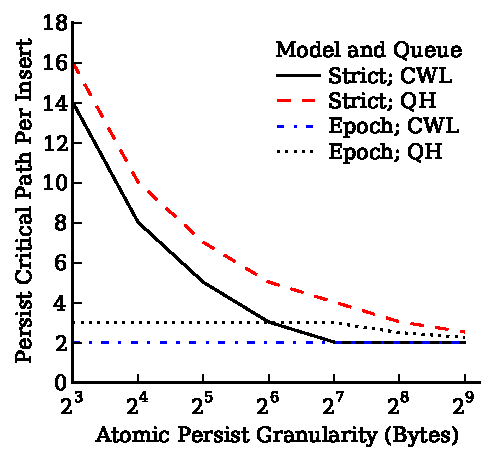
\includegraphics[width=.55\linewidth]{PersistencyEval/Coalescing.pdf}
  \caption{\textbf{Atomic Persist Size.} 1 Thread. Large atomic persists allow coalescing, increasing persist concurrency.  While effective for strict persistency, large atomic persists do not improve persist concurrency for relaxed models.}
  \label{fig::Coalescing}
\end{figure}


Figure~\ref{fig::Coalescing} displays average persist ordering critical path per insert for \emph{Copy While Locked} and \emph{Queue Holes} for both strict persistency and epoch persistency as atomic persist size increases from eight to 512 bytes.
At eight-byte persists there is a large separation between strict persistency and epoch persistency.
As atomic persist size increases the persist critical path of strict persistency steadily decreases while the critical path of epoch persistency remains largely unchanged.
At 512-byte atomic persists (right of the Figure) strict persistency matches epoch persistency.
For these queue benchmarks larger atomic persists provide the same improvement to persist critical path as relaxed persistency, but offer no improvement to relaxed models.
Increasing atomic persist granularity offers an alternative to relaxed persistency models.

\textbf{Persist False Sharing.}
Just as in existing memory systems, persists suffer from false sharing, degrading performance.
False sharing traditionally occurs under contention to the same cache line even though threads access disjoint addresses in that cache line.
Similarly, \emph{persistent false sharing} occurs when a persist ordering constraint is unnecessarily introduced due to the coarseness at which races are observed.
Persistent false sharing occurs in races to both persistent and volatile memory, as races to both address spaces establish persist ordering constraints.

 \begin{figure}
  \centering
  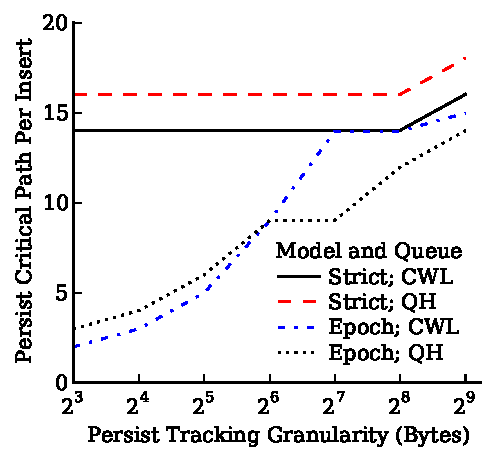
\includegraphics[width=.55\linewidth]{PersistencyEval/FalseSharing.pdf}
  \caption{\textbf{Persistent False Sharing.} 1 Thread.  False sharing negligably affects strict persistency (persists already serialized); relaxed models reintroduce constraints.}
  \label{fig::FalseSharing}
\end{figure}


Figure~\ref{fig::FalseSharing} shows average persist critical path per insert for \emph{Copy While Locked} and \emph{Queue Holes} for both strict persistency and epoch persistency as the granularity at which persist ordering constraints propagate increases.
For fine-grained tracking epoch persistency provides a far lower persist critical path than strict persistency.
As tracking granularity increases, strict persistency performance remains the same while epoch persistency decreases (critical path increases).
At 512-byte tracking granularity strict persistency and epoch persistency provide comparable persist critical paths; many of the persist constraints removed by relaxing consistency are reintroduced through false sharing.

\section{Future Work}
\label{sec:PersistencyEval:FutureWork}

This dissertation lays the foundation for reasoning about NVRAM performance and programming interfaces, culminating in memory persistency.
However, I leave it to future work to investigate how best to use persistency to build recoverable systems with NVRAM.

\textbf{Software for NVRAM.}
NVRAM should eventually allow data structures with the performance of existing DRAM systems but that recover after failures.
Such software will require transformations to introduce logs or indirection, and to properly order writes.
These transformations slow execution on even volatile memory systems.
However, an instruction-direct memory interface holds the potential to improve execution beyond block and transaction interfaces by increasing thread concurrency and removing frequent copies inherent in block storage interfaces.

New data structures must be developed to bridge the gap between existing high performance main-memory versions and those that provide recovery with disk.
For example, ordered indexes are typically implemented as B+Trees with disk, but novel (and complicated) variations exist for main memory, such as highly concurrent balanced trees and lock-free skip lists.
With NVRAM and memory persistency one might imagine a recoverable lock-free tree or skip list with bounded recovery time.
How to design such data structures remains uncertain, as does their true performance potential.

\textbf{New models and hardware implementations.}
Once software has been designed we will require hardware implementations of persistency models and NVRAM memory systems.
Existing memory consistency encompasses a broad literature of models and implementations, detailing specific relaxations to improve performance.
High performance techniques involving speculation further improve performance for strict consistency models.
The same will be true for persistency models, yet I expect persistency models must be further relaxed compared to consistency models (an NVRAM persist may take an order of magnitude longer than making a store visible to other processors).
Akin to speculation, logging and indirection (such as copy-on-write) may improve performance of strict persistency models.

Designing high performance and highly concurrent data structures, even without regard for persistency, remains a challenge.
To simplify matters researchers have introduced ``programmer-centric" memory consistency models---models that provide the appearance of SC when certain criteria are met (e.g., data-race-free-zero \cite{Adve96}).
Memory persistency may be similarly simplified by identifying programming patterns and the minimal synchronization constructs to present the appearance of SC while still giving the compiler and processor as much freedom as possible to reorder persists.

\textbf{Implementing efficient persist coalescing.}
Finally, the previous chapters assume that coalescing will be an important feature of NVRAM systems; indeed, recent work has already demonstrated that without hardware coalescing the software must cache and coalesce persists, introducing additional instructions and increasing the likelihood of design errors \cite{ConditNightingale09,FangHsiao11}.
Coalescing presents several problems such as detecting when coalescing is allowable and determining how long persists should be delayed (delaying a persist increases the chance that it will coalesce with future persists, but may delay important events such as transaction commit).
Future work must investigate language, compiler, and hardware mechanisms to provide persist coalescing.
It is possible for coalescing to occur only under specific conditions (e.g., coalescing only occurs between persists on the same thread, coalescing only occurs to a limited number of addresses labeled by the programmer), reducing hardware complexity.

\section{Conclusion}
\label{sec:PersistencyEval:Conclusion}

Future NVRAM technologies offer the performance of DRAM with the durability of disk.
However, existing memory interfaces are incapable of guaranteeing proper data recovery by properly enforcing persist order.
In previous chapters I introduced \emph{memory persistency}, an extension to memory consistency that allows programmers to describe persist order constraints.
Additionally, I outlined the design space of possible memory persistency models and detailed three persistency models and their use in implementing a persistent queue.
In this chapter I use memory tracing and simulation to demonstrate that strict persistency models suffer a 30$\times$ slowdown relative to instruction execution rate, and that relaxed persistency effectively regains this performance.
Memory persistency represents a framework for defining programmer interfaces for NVRAM and reasoning about program correctness for recoverable applications.


\startappendices
 \appendix{Understanding and Abstracting Total Data Center Power}
 \label{app:WEED}
 %\documentclass[a4paper]{acm_proc_article-sp}

%\usepackage{setspace}  % For single/double spacing
%\usepackage{booktabs}
%\usepackage{tabularx}
%\usepackage{times} % For times font
%\usepackage{subfigure}
%\usepackage{xspace} 
%\usepackage[numbers,square,sort]{natbib} 
%\usepackage[usenames]{color}
%\usepackage[margin=.9in]{geometry}

%\hyphenation{component\-by\-compo-nent}

%\begin{document}

%\addtolength{\topmargin}{-.25 in}
%\addtolength{\textheight }{.5 in}


 \newcommand{\simname}{Simulation Name}
 \newcommand{\modelname}{Model Name}

 \newcommand{\U}{$U$\xspace}
 \newcommand{\usrv}{$u_{Srv}$\xspace}
 \newcommand{\Toutside}{$T_{\mathrm{Outside}}$\xspace}
 \newcommand{\el}{$\ell$\xspace}

%\newcommand{\fixme}[1]{\textbf{\textcolor{red}{[ Fixme: #1]}}}
%\newcommand{\needref}{\textcolor{red}{[ref]}\xspace}

% \twocolumn[%
% \centerline{\huge Understanding and Abstracting Total Data Center Power}
% 
%    \medskip
%
%
% \centerline{ \large Steven Pelley$^\dagger$  \hspace{.3 in} David Meisner$^\dagger$ \hspace{.3 in}  Thomas F. Wenisch$^\dagger$ \hspace{.3 in} James W. VanGilder$^\ddagger$}
% 
%   \medskip
% 
%  
%\centerline{ \large \{spelley, meisner, twenisch\}@umich.edu \hspace{.3 in} Jim.VanGilder@apc.com}
% 
%   \medskip
%
% \centerline{ \large \hspace{.1 in} $^\dagger$Advanced Computer Architecture Lab \hspace{.3 in} $^\ddagger$APC by Schneider Electric}
%\centerline{ \large  \hspace{.1 in} The University of Michigan \hspace{2.3 in}}
%
% \bigskip
% 
% ]
%
% \vspace{ .1in}

% appendix authors
{
\centering
Steven Pelley, David Meisner, Thomas F. Wenisch, and James W. VanGilder \\
\vspace{2\baselineskip}
}
 
 
%\small


%\singlespacing
%\vspace{-0.7in}
%\begin{abstract}
%\small
\emph{Data center power infrastructure incurs massive capital costs, which typically exceed energy costs over the life of the facility. To squeeze maximum value from the infrastructure, researchers have proposed over-subscribing power circuits, relying on the observation that peak loads are rare.  To ensure availability, these proposals employ} power capping, \emph{which throttles server performance during utilization spikes to enforce safe power budgets.  However, because budgets must be enforced locally---at each power distribution unit (PDU)---local utilization spikes may force throttling even when power delivery capacity is available elsewhere.  Moreover, the need to maintain reserve capacity for fault tolerance on power delivery paths magnifies the impact of utilization spikes.}

\emph{In this paper, we develop mechanisms to better utilize installed power infrastructure, reducing reserve capacity margins and avoiding performance throttling. Unlike conventional high-availability data centers, where collocated servers share identical primary and secondary power feeds, we reorganize power feeds to create} shuffled \emph{power distribution topologies. Shuffled topologies spread secondary power feeds over numerous PDUs, reducing reserve capacity requirements to tolerate a single PDU failure.  Second, we propose} Power Routing, \emph{which schedules IT load dynamically across redundant power feeds to: (1) shift slack to servers with growing power demands, and (2) balance power draw across AC phases to reduce heating and improve electrical stability.  We describe efficient heuristics for scheduling servers to PDUs (an NP-complete problem). Using data collected from nearly 1000 servers in three production facilities, we demonstrate that these mechanisms can reduce the required power infrastructure capacity relative to conventional high-availability data centers by 32\% without performance degradation.}

%%%\end{abstract}
%%%
%%%\normalsize
%%%
%%%\category{C.5.5}{Computer System Implementation}{Servers}
%%%
%%%\terms
%%%Design, Measurement
%%%
%%%\keywords
%%%power infrastructure, data centers



\section{Introduction}

Data center power consumption continues to grow at an alarming pace; it is projected to reach 100 billion kWh at an annual cost of \$7.4 billion within two years \cite{EPA07}, with a world-wide carbon-emissions impact similar to that of the entire Czech Republic \cite{Mankoff08}. In light of this trend, computer systems researchers, application designers, power and cooling engineers, and governmental bodies have all launched research efforts to improve data center energy efficiency.  These myriad efforts span numerous aspects of data center design (server architecture \cite{Lefurgy03,Meisner09}, scheduling \cite{Moore06, Parolini08},  power delivery systems \cite{Fan07}, cooling infrastructure \cite{Patel02}, etc.).  However, with few exceptions, existing efforts focus narrowly on energy-efficiency of single subsystems, without considering global interactions or implications across data center subsystems. 

As sophisticated power management features proliferate, the dynamic range of data center power draw (as a function of utilization) is increasing, and interactions among power management strategies across subsystems grow more complex; subsystems can no longer be analyzed in isolation.   Even questions that appear simple on their face can become quite complicated.

Reasoning about total data center power is difficult because of the diversity and complexity of data center infrastructure.  Five distinct sub-systems (designed and marketed by different industry segments) account for most of a data center's power draw:  (1) servers and storage systems, (2) power conditioning equipment, (3) cooling and humidification systems, (4) networking equipment, and (5) lighting/physical security.  Numerous sources have reported power breakdowns \cite{EPA07,Meisner09}; Table~\ref{table::PowerDistribution} illustrates a typical breakdown today.   The first three subsystems dominate and their power draw can vary drastically with data center utilization. Cooling power further depends on ambient weather conditions around the data center facility. Even the distribution of load in each subsystem can affect power draws, as the interactions among sub-systems are non-linear
%(e.g., thermal hot spots disproportionately increase cooling requirements).

In this paper, our objective is to provide tools to the computer systems community to assess and reason about total data center power.  Our approach is two-fold, targeting both \emph{data center simulation} and \emph{abstract analytic modeling}.  First, we have collected a set of detailed power models (from academic sources, industrial white papers, and product data sheets) for each critical component of data center infrastructure, which describe power draw as a function of environmental and load parameters.  Each model describes the power characteristics of a single device (i.e., one server or computer room air handler (CRAH)) and, as such, is suitable for integration into a detailed data center simulator.  We describe how these models interact (i.e., how utilization, power, and heat flow among components) and outline the design of such a simulator. To our knowledge, we are the first to describe an integrated data center simulation infrastructure; its implementation is underway.

Although these detailed models enable data center simulation, they do not allow direct analytic reasoning about total data center power.  Individual components' power draw vary non-linearly with localized conditions (i.e., temperature at a CRAH inlet, utilization of an individual server), that require detailed simulation to assess precisely.  Hence, to enable back-of-the-envelope reasoning, we develop an \emph{abstract model} that replaces key steps of the data center simulation process with simple parametric models that enable analysis of average behavior.  In particular, we abstract away time-varying scheduling/load distribution across servers and detailed tracking of the thermodynamics of data center airflow.  Our abstract model provides insight into how data center sub-systems interact and allows quick comparison of energy-efficiency optimizations.

\begin{table}[t]
\begin{center}
\caption{ \textbf{Typical Data Center Power Breakdown.} }
\label{table::PowerDistribution}

\begin{tabularx}{\linewidth}{c c c c c}
    \toprule
    Servers & Cooling & Power Cond. & Network & Lighting \\
    \midrule
    56\% & 30\% & 8\% & 5\% & 1\% \\
    \bottomrule
  \end{tabularx}
\end{center}

\end{table}


\begin{figure*}[!ht]
\centering
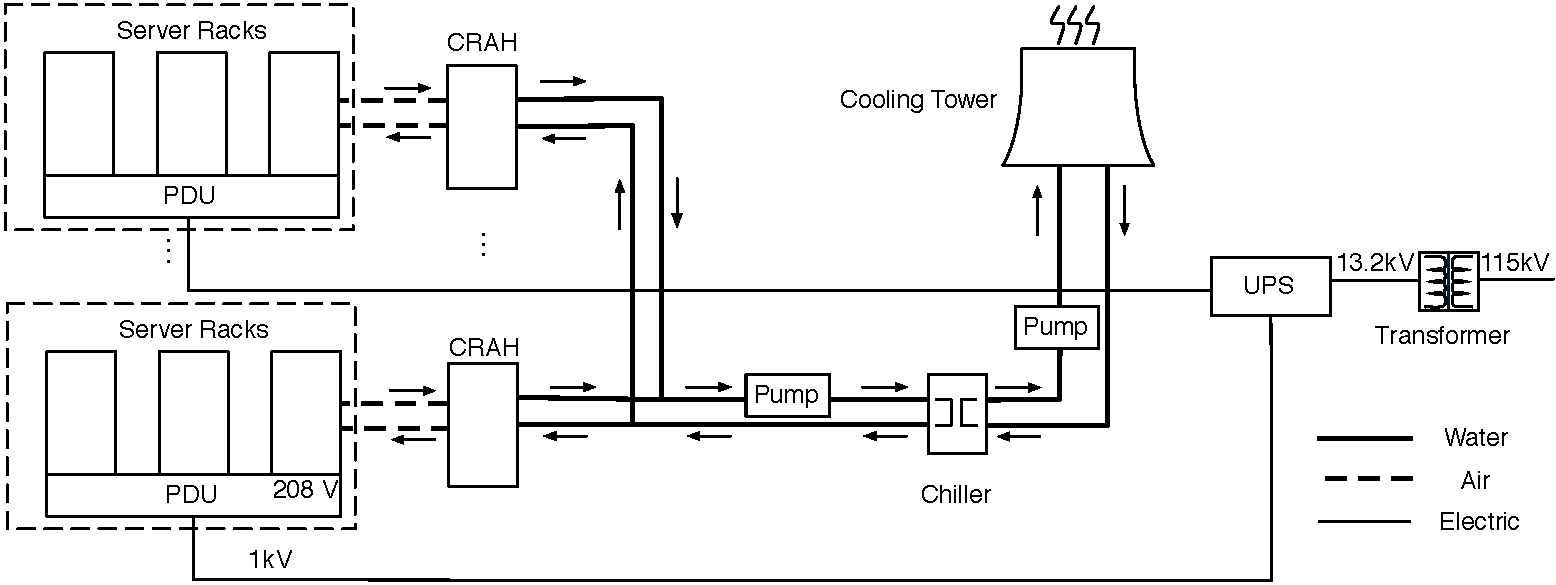
\includegraphics[width = 6.5 in]{Appendices/WEED/figure/HeatFlow.pdf}
\caption{ \textbf{Power and Cooling Flow.} }
\label{figure::PowerFlow}
\vspace{-.1 in}
\end{figure*}

\section{Related Work}

%{\bf Modeling system power}

The literature on computer system power management is vast; a recent survey appears in \cite{KaxirasBook08}.  A tutorial on data center infrastructure and related research issues is available in \cite{BarrosoBook09}.  

Numerous academic studies and industrial whitepapers describe or apply models of power draw for individual data center subsystems.  Prior modeling efforts indicate that server power varies roughly linearly in CPU utilization \cite{Fan07,Rivoire08}. Losses in power conditioning systems and the impact of power overprovisioning are described in \cite{Fan07, Rasmussen113}. Our prior work proposes mechanisms to eliminate idle power waste in servers \cite{Meisner09}.  Other studies have focused on understanding the thermal implications of data center design  \cite{Heath06, Patel02}.  Power- and cooling-aware scheduling and load balancing can mitigate data center cooling costs  \cite{Moore06, Parolini08}.  Though each of these studies examines particular aspects of data center design, none of these present a comprehensive model for total data center power draw.  

%{\bf Modeling thermal}






\vspace{0.1 in}
\section{Data Center Power Flow}

We begin by briefly surveying major data center subsystems and their interactions. Figure  \ref{figure::PowerFlow} illustrates the primary power-consuming subsystems and how power and heat flow among them.  Servers (arranged in racks) consume the dominant fraction of data center power, and their power draw varies with utilization.  

The data center's power conditioning infrastructure typically accepts high-voltage AC power from the utility provider, transforms its voltage, and supplies power to uninterruptible power supplies (UPSs).  The UPSs typically charge continuously and supply power in the brief gap until generators can start during a utility failure.   From the UPS, electricity is distributed at high voltage (480V-1kV) to power distribution units (PDUs), which  regulate voltage to match IT equipment requirements.  Both PDUs and UPSs impose substantial power overheads, and their overheads grow with load. 

Nearly all power dissipated in a data center is converted to heat, which must be evacuated from the facility.  Removing this heat while maintaining humidity and air quality requires an extensive cooling infrastructure.  Cooling begins with the computer room air handler (CRAH), which transfer heat from servers' hot exhaust to a chilled water/glycol cooling loop while supplying cold air throughout the data center.
CRAHs appear in various forms, from room air conditioners that pump air through underfloor plenums to in-row units located in containment systems.
The water/glycol heated by the CRAHs is then pumped to a chiller plant where heat is exchanged between the inner water loop and a second loop connected to a cooling tower, where heat is released to the outside atmosphere.
Extracting heat in this manner requires substantial energy; chiller power dominates overall cooling system power, and its requirements grow with both the data center thermal load and outside air temperature. 


%Within a data center the power that each component uses varies substantially.
%Ideally, nearly all power would be consumed by the IT equipment.
%In reality, the other devices frequently draw the majority of power.
%Figure  \ref{figure::PowerFlow} shows the power distribution of a typical highly available dual-power-path data center with N+1 CRAC units.
%The data center under consideration runs at 30\% of peak capacity.
%Only 30\% of the eletrical power in reaches the servers, corresponding to a PUE of 3.33.
%The cooling system as a whole consumes 45\% of total power, the majority by the chiller plant.
%23\% of the power is lost by the power conditioning equipment.
%Finally, fixed-cost facilities such as lighting account for the final 2\%.



%Data center power draw varies primarily as a function of total data center utilization and external ambient temperature.
%Figure \ref{figure::Dependencies} shows how the various components effect each other's power draw.
%The total load directly determines the power needed by the servers and IT equipment.
%All of this power must be provided through the power conditioning system - UPS and PDU.
%As the power draw in the UPS and PDU is electrical loss, the power conditioning system as a whole accounts for power draw roughly proportional to total data center utilization.
%The servers and power conditioning equipment together produce heat that must be removed by the cooling system.
%Each component of the cooling system requires power that grows superlinear with the heat to be removed.
%Thus, the overall cooling power necessary will increase as utilization increases.
%Additionally, the power required by the chiller greatly increases as the outside ambient air temperature rises.


%Numerous components in a data center consume power.
%Generally, devices can be characterized as part of the electrical infrastructure or cooling infrastructure.
%See Figure \ref{figure::PowerFlow} for a depiction of typical data center components.
%In order to meet the high power demands of servers, data centers require power distribution units (PDU) capable of transforming and regulating voltages.
%As can be seen, each PDU supports a number of racks in the computer room.
%Additionally, uninterruptable power supplies (UPS) are necessary to ensure the availability of servers and other computing resources in the event of a power failure.
%Together, the servers, PDU, and UPS generate excessive amounts of heat, requiring an extensive cooling infrastructure.
%Cooling begins with the computer room air conditioner (CRAC).
%The CRAC blows air through the computer room, transfering heat from the warm computer room air to a chilled water or glycol supply.
%The liquid is pumped to a chiller plant where heat is exchanged between the inner water loop and a second loop connected to a cooling tower.
%The chiller must provide the cooling tower with water hotter than the outside air in order for heat to transfer from the cooling tower to the atmosphere.
%As the outside temperature increases, the chiller consumes more energy.
%During design, sufficient resources must be accounted for in order to power and cool the data center at peak utilization.
%It is important to realize that nearly every component discussed here runs less efficiently at lower loads.
%Understanding the power and cooling requirements of each of these components is central to developing a comprehensive model of data center power consumption.

%We construct a model for the total data center power draw by developing detailed component-wise models for each of the primary power-consuming components of a data center.
%We base each component model on existing models captured in computer engineering and ASHRAE literature as well as manufacturer spec sheets.
%In order to understand data center power usage, it is important to decompose the various sub-systems and their unique purposes and power consumption characteristics.


\section{Modeling Data Center Power} 
\label{section:Model}


Our objective is to model total data center power at two granularities: for detailed simulation and for abstract analysis.  Two external factors primarily affect data center power usage: the aggregate load presented to the compute infrastructure and the ambient outside air temperature (outside humidity secondarily affects cooling power as well, but, to limit model complexity, we do not consider it here).  We construct our modeling framework by composing models for the individual data center components.  In our abstract models, we replace key steps that determine the detailed distribution of compute load and heat with simple parametric models that enable reasoning about average behavior.

\begin{table}[t]
\centering
\caption{ \textbf{Variable Definitions.} }
\label{table::VariableDefinitions}
%\begin{tabularx}{\linewidth}{r l r l}
\begin{tabular}{r l r l}
   \toprule
    $U$ & Data Center Utilization  & $T$ & Temperature \\
    $u$ & Component Utilization & $\dot{m}$ & Flow Rate \\
    $\kappa$ & Containment Index & $C_{\mathrm{p}}$ & Heat Capacity \\
    $\ell$ & Load Balancing Coefficient & $N_{\mathrm{Srv}}$ & \# of Servers \\
    $E$ & Heat Transfer Effectiveness & $P$ & Power \\
    $\pi$ & Loss Coefficient & $q$ & Heat \\
    $f$ & Fractional Flow Rate & & \\

    %$T$ & Temperature \\
    %$\dot{m}_{\mathrm{air}}$ & Volumetric Flow Rate of Air \\
    %$C_{\mathrm{p}_{\mathrm{air}}}$ & Specific Heat Capacity of Air \\
    %$\kappa$ & Containment Index \\
    %$E$ & Heat Transfer Effectiveness \\
    %$\dot{m}_{\mathrm{F}}$ & Fractional Volumetric Flow Rate \\
   \bottomrule
  \end{tabular}
  %\end{tabularx}
\end{table}

{\bf Framework.}  We formulate total data center power draw, $P_{\mathrm{Total}}$, as a function of total utilization, \U, and ambient outside temperature, \Toutside.  Figure \ref{figure::DataFlow} illustrates the various intermediary data flows and models necessary to map from \U and \Toutside to $P_{\mathrm{Total}}$. Each box is labeled with a sub-section reference that describes that step of the modeling framework.  In the left column, the power and thermal burden generated by IT equipment is determined by the aggregate compute infrastructure utilization, \U.  On the right, the cooling system consumes power in relation to both the heat generated by IT equipment and the outside air temperature.


{\bf Simulation \& Modeling.} In simulation, we relate each component's utilization (processing demand for servers, current draw for electrical conditioning systems, thermal load for cooling systems, etc.) to its power draw on a component-by-compo\-nent basis.  Hence, simulation requires precise accounting of per-component utilization and the connections between each component.  For servers, this means knowledge of how tasks are assigned to machines; for electrical systems, which servers are connected to each circuit; for cooling systems, how heat and air flow through the physical environment.  We suggest several approaches for deriving these utilizations and coupling the various sub-systems in the context of a data center simulator; we are currently developing such a simulator.

However, for high-level reasoning, it is also useful to model aggregate behavior under typical-case or parametric assumptions on load distribution. Hence, from our detailed models, we construct abstract models that hide details of scheduling and topology.

\begin{figure}[t!]
\centering
\includegraphics[width = 3 in]{Appendices/WEED/figure/Dependencies.pdf}
\caption{ \textbf{Data Flow.} }
\label{figure::DataFlow}
\end{figure}

{\bf 4.1. Abstracting Server Scheduling.}

The first key challenge in assessing total data center power involves characterizing server utilization and the effects of task scheduling on the power and cooling systems.  Whereas a simulator can incorporate detailed scheduling, task migration, or load balancing mechanisms to derive precise accounting of per-server utilization, we must abstract these mechanisms for analytic modeling.

As a whole, our model relates total data center power draw to aggregate data center utilization, denoted by \U.  Utilization varies from 0 to 1, with 1 representing the peak compute capacity of the data center.  We construe \U as unitless, but it might be expressed in terms of number of servers, peak power (Watts), or compute capability (MIPS).
%Total data center power is the sum of subsystem power draws---servers, power conditioning, cooling, networking, and overhead, each itself a function of \U.
For a given \U, individual server utilizations may vary (e.g., as a function of workload characteristics, consolidation mechanisms, etc.). We represent the per-server utilizations with \usrv, where the subscript indicates the server in question.
For a homogeneous set of  servers:

\begin{equation}
 U = \frac{1}{N_{\mathrm{Srv}}}\sum_{\mathrm{Servers}}u_{\mathrm{Srv}[i]}
\end{equation}

For simplicity, we have restricted our analytic model to a homogeneous cluster.
In real data centers, disparities in performance and power characteristics across servers require detailed simulation to model accurately, and their effect on cooling systems can be difficult to predict \cite{Nathuji08}.

%As we shall see, server power draw is non-linear in \U.  In particular, one might consolidate workloads and turn servers off when \U is low, conserving idle power. Hence, precisely how \U decomposes into per-server power draws is critical to total power requirements.

To abstract the effect of consolidation, we characterize the individual server utilization, \usrv, as a function of \U and a measure of task consolidation, \el.  We use \el to capture the degree to which load is concentrated or spread over the data center's servers. For a given \U and \el we define individual server utilization as:

\begin{equation}
u_{\mathrm{Srv}} = \frac{U}{U + (1-U)\ell}
\end{equation}

\usrv only holds meaning for the $N_{\mathrm{Srv}}(U + (1-U)\ell)$  servers that are non-idle; the remaining servers have zero utilization, and are assumed to be powered off. Figure \ref{figure::ServerUtilization} depicts the relationship among \usrv, \U, and \el.
$\ell = 0$ corresponds to perfect consolidation---the data center's workload is packed onto the minimum number of servers, and the utilization of any active server is 1. $\ell = 1$ represents the opposite extreme of perfect load balancing---all servers are active with \usrv~=~\U.  Varying \el allows us to represent consolidation between these extremes. 

%\begin{figure}[t!]
%  \centering
%  \includegraphics[width = 3.5 in]{figure/LoadBalancingCoeff.pdf}
%  \caption{ \textbf{ Server Utilization. } }
%  \label{figure::ServerUtilization}
%\end{figure}



{\bf 4.2. Server Power.} 

Several studies have characterized server power consumption \cite{BarrosoBook09,Fan07,Meisner09,Rivoire08}.
Whereas the precise shape of the utilization-power relationship varies, servers generally consume roughly half of their peak load power when idle, and power grows with utilization.
In line with prior work \cite{Rivoire08}, we approximate a server's power consumption as linear in utilization between a fixed idle power and peak load power.

\begin{equation}
P_{\mathrm{Srv}} = P_{\mathrm{Srv}_{\mathrm{Idle}}} + ( P_{\mathrm{Srv}_{\mathrm{Peak}}} - P_{\mathrm{Srv}_{\mathrm{Idle}}}) u_{\mathrm{Srv}}
\end{equation}

%In actuality, power draw depends on per-component utilization within the server.  Various components
%exhibit a variety of power to utilization relationships (near constant to quadratic).
%However, CPU utilization is a good approximation for overall system utilization for most workloads  \cite{Rivoire08}.

%\begin{figure}[t!]
%  \centering
%  \includegraphics[width = 3.5 in]{figure/spec.pdf}
%  \caption{ \textbf{ Server Power. } }
%  \label{figure::Spec}
%\end{figure}

Power draw is not precisely linear in utilization; server sub-components exhibit a variety of relationships (near constant to quadratic).
It is possible to use any nonlinear analytical power function, or even a suitable piecewise function.
Additionally, we have chosen to use CPU utilization as an approximation for overal system utilization; a more accurate representation of server utilization might instead be employed.
In simulation, more precise system/workload-specific power modeling is possible by interpolating in a table of measured power values at various utilizations (e.g., as measured with the SpecPower benchmark).
Figure \ref{figure::Spec} compares the linear approximation against published SpecPower results for two recent Dell systems.

{\bf 4.3. Power Conditioning Systems.} 

Data centers require considerable infrastructure simply to distribute uninterrupted, stable electrical power.  PDUs transform the high voltage power distributed throughout the data center to voltage levels appropriate for servers. They incur a constant power loss as well as a power loss proportional to the square of the load \cite{Rasmussen113}:

\begin{equation}
P_{\mathrm{PDU}_{\mathrm{Loss}}} = P_{\mathrm{PDU}_{\mathrm{Idle}}} + \pi_{\mathrm{PDU}}(\sum_{Servers}P_{\mathrm{Srv}})^{2}
\end{equation}

where $P_{\mathrm{PDU}_{\mathrm{Loss}}}$ represents power consumed by the PDU, $\pi_{\mathrm{PDU}}$ represents the PDU power loss coefficient, and $P_{\mathrm{PDU}_{\mathrm{Idle}}}$ the PDU's idle power draw. PDUs typically waste 3\% of their input power.
As current practice requires all PDUs to be active even when idle, the total dynamic power range of PDUs for a given data center utilization is small relative to total data center power; we chose not to introduce a separate PDU load balancing coefficient and instead assume perfect load balancing across all PDUs.

UPSs provide temporary power during utility failures.  UPS systems are typically placed in series between the utility supply and PDUs and impose some power overheads even when operating on utility power.  UPS power overheads follow the relation \cite{Rasmussen113}:

\begin{equation}
P_{\mathrm{UPS}_{\mathrm{Loss}}} = P_{\mathrm{UPS}_{\mathrm{Idle}}} + \pi_{\mathrm{UPS}}\sum_{PDUs}P_{\mathrm{PDU}}
\end{equation}

where $\pi_{\mathrm{UPS}}$ denotes the UPS loss coefficient.  UPS losses typically amount to 9\% of their input power at full load.

%\begin{figure}[t!]
%  \centering
%  \includegraphics[width = 3.5 in]{figure/PowerConditioning.pdf}
%  \caption{ \textbf{ Power Conditioning Losses } }
%  \label{figure::PowerConditioning}
%\end{figure}

%
%\begin{figure*}[ht]
%\centering

%\subfigure[\textbf{ Server Utilization. }]{
%  \includegraphics[width = 2 in]{figure/LoadBalancingCoeff.pdf}
%  \label{figure::ServerUtilization}
%}

%\subfigure[\textbf{ Server Power. } ]{
%  \includegraphics[width = 2 in]{figure/spec.pdf}
%  \label{figure::Spec}
%}

%\subfigure[\textbf{ Power Conditioning Losses }]{
%  \includegraphics[width = 2 in]{figure/PowerConditioning.pdf}
%  \label{figure::PowerConditioning}
%}

%\end{figure*}


\begin{figure*}[ht]

%\begin{minipage}[b]{0.5\linewidth}

\begin{minipage}[b]{.5\linewidth}
  \centering
  \includegraphics[width=\linewidth]{Appendices/WEED/figure/LoadBalancingCoeff.pdf}
  \caption{\textbf{ Individual Server Utilization. }}
  \label{figure::ServerUtilization}
\end{minipage}
\begin{minipage}[b]{0.5\linewidth}
  \centering
  \includegraphics[width = \linewidth]{Appendices/WEED/figure/spec.pdf}
  \caption{\textbf{ Individual Server Power. } }
  \label{figure::Spec}
\end{minipage}
\begin{minipage}[b]{0.5\linewidth}
\centering
  \includegraphics[width = \linewidth]{Appendices/WEED/figure/PowerConditioning.pdf}
\caption{\textbf{ Power Conditioning Losses. }}
  \label{figure::PowerConditioning}
\end{minipage}

\end{figure*}

%Because they are in series, PDU and UPS losses compound.
Figure \ref{figure::PowerConditioning} shows the power losses for a 10MW (peak server power) data center.
At peak load, power conditioning loss is 12\% of total server power.  Furthermore, these losses result in additional heat that must be evacuated by the cooling system.

{\bf 4.4. Heat and Air Flow.} 

Efficient heat transfer in a data center relies heavily on the CRAH's ability to provide servers with cold air.  
CRAHs serve two basic functions: (1) to provide sufficient airflow to prevent recirculation of hot server exhaust to server inlets, and (2) to act as a heat exchanger between server exhaust and some heat sink, typically chilled water.

In general, heat is transferred between two bodies according to the following thermodynamic principle:

\begin{equation}
q = \dot{m} C_{\mathrm{p}} ( T_{\mathrm{h}} - T_{\mathrm{c}})
\end{equation}

Here $q$ is the power transferred between a device and fluid, $\dot{m}$ represents the fluid mass flow, and $C_{\mathrm{p}}$ is the specific heat capacity of the fluid.
$T_{\mathrm{h}}$ and $T_{\mathrm{c}}$ represent the hot and cold temperatures, respectively.
The values of $\dot{m}$, $T_{\mathrm{h}}$, and $T_{\mathrm{c}}$ depend on the physical air flow throughout the data center and air recirculation.

Air recirculation arises when hot and cold air mix before being ingested by servers, requiring a lower cold air temperature and greater mass flow rate to maintain server inlet temperature within a safe operating range.
%Even a small amount of recirculation can require a several degree reduction in CRAH cold-air supply temperature to avoid local hot spots and server overheating.
Data center designers frequently use computational fluid dynamics (CFD) to model the complex flows that arise in a facility and lay out racks and CRAHs to minimize recirculation.  The degree of recirculation depends greatly on data center physical topology, use of containment systems, and the interactions among high-velocity equipment fans.  In  simulation, it is possible to perform CFD analysis to obtain accurate flows. 

For abstract modeling, we replace CFD with a simple parametric model of recirculation that can capture its effect on data center power.  We introduce a \emph{containment index} ($\kappa$), based on previous metrics for recirculation \cite{Tozer09, VanGilder07}.
Containment index is defined as the fraction of air ingested by a server that is supplied by a CRAH (or, at the CRAH, the fraction that comes from server exhaust).
The remaining ingested air is assumed to be recirculated from the device itself.
Thus, a $\kappa$ of 1 implies no recirculation (a.k.a. perfect containment).
Though containment index varies across servers and CRAHs (and may vary with changing airflows), our abstract model uses a single, global containment index to represent average behavior, resulting in the following heat transfer equation:

\begin{equation}
q  = \kappa \dot{m}_{\mathrm{air}} C_{\mathrm{p}_{\mathrm{air}}} ( T_{\mathrm{a}_\mathrm{h}} - T_{\mathrm{a}_\mathrm{c}})
\label{equation::HeatTransfer}
\end{equation}

%\begin{figure}[t!]
%  \centering
%  \includegraphics[width = 3.5 in]{figure/AirFlow1CRAHSupply.pdf}
%  \caption{ \textbf{ Effects of $\kappa$ and u on air flow } }
%  \label{figure::AirFlow}
%\end{figure}
\begin{figure*}[ht]

%\begin{minipage}[b]{0.5\linewidth}

\begin{minipage}[b]{0.5\linewidth}
  \centering
  \includegraphics[width = \linewidth]{Appendices/WEED/figure/AirFlow1CRAHSupply.pdf}
  \caption{ \textbf{ CRAH Supply Temperature. } }
  \label{figure::AirFlow}
\end{minipage}
\begin{minipage}[b]{0.5\linewidth}
\centering
  \includegraphics[width = \linewidth]{Appendices/WEED/figure/CRAH1CI.pdf}
  \caption{ \textbf{ CRAH Power. } }
  \label{figure::CRAH}
\end{minipage}
\begin{minipage}[b]{0.5\linewidth}
  \centering
 \includegraphics[width = \linewidth]{Appendices/WEED/figure/ChillerCHWSvaryQ.pdf}
   \caption{ \textbf{ Chilled Water Temperature.} }
  \label{figure::ChillerA}
\end{minipage}

\end{figure*}
For this case, $q$ is the heat transferred by the device (either server or CRAH), $\dot{m}_{\mathrm{air}}$ represents the total air flowing through the device, $T_{\mathrm{a}_{\mathrm{h}}}$ the temperature of the air exhausted by the server, and $T_{\mathrm{a}_{\mathrm{c}}}$ is the temperature of the cold air supplied by the CRAH.  These temperatures represent the hottest and coldest air temperatures in the system, respectively, and are not necessarily the inlet temperatures observed at servers and CRAHs (except for the case when $\kappa = 1$).

Using only a single value for $\kappa$ simplifies the model by allowing us to enforce the conservation of air flow between the CRAH and servers.
Figure \ref{figure::AirFlow} demonstrates the burden air recirculation places on the cooling system. We assume flow through a server increases linearly with server utilization (representing variable-speed fans) and a peak server power of 200 watts.
The left figure shows the CRAH supply temperature necessary to maintain the typical maximum safe server inlet temperature of 77$^{\circ}$F.  As $\kappa$ decreases, the required CRAH supply temperature quickly drops.  Moreover, required supply temperature drops faster as utilization approaches peak.  As we show next, lowering supply temperature results in super-linear increases in CRAH and chiller plant power.
Preventing air recirculation (e.g., with containment systems) can drastically improve cooling efficiency.

{\bf 4.5. Computer Room Air Handler.} 

CRAHs transfer heat out of the server room to the chilled water loop.  We model this exchange of heat using a modified effectiveness-NTU method \cite{Cengel03}:

\begin{equation}
q_{\mathrm{crah}} = E \, \kappa  \,\dot{m}_{\mathrm{air}} C_{\mathrm{p}_\mathrm{air}} f^{0.7} (\kappa \, T_{\mathrm{a}_\mathrm{h}} + (1-\kappa) T_{\mathrm{a}_\mathrm{c}} - T_{\mathrm{w}_\mathrm{c}})
\end{equation}

$q_{\mathrm{crah}}$ is the heat removed by the CRAH, $E$ is the transfer efficiency at the maximum mass flow rate (0 to 1), $f$ represents the volume flow rate as a fraction of the maximum volume flow rate, and $T_{\mathrm{w}_\mathrm{c}}$ the chilled water temperature.

CRAH power is dominated by fan power, which grows with the cube of mass flow rate to some maximum, here denoted as $P_{\mathrm{CRAH}_{\mathrm{Dyn}}}$.
Additionally, there is some fixed power cost for sensors and control systems, $P_{\mathrm{CRAH}_{\mathrm{Idle}}}$.  We model CRAH units with variable speed drives (VSD) that allow volume flow rate to vary from zero (at idle) to the CRAH's peak volume flow.  Some CRAH units are cooled by air rather than chilled water or contain other features such as humidification systems which we do not consider here.

\begin{equation}
P_{\mathrm{CRAH}} = P_{\mathrm{CRAH}_{\mathrm{Idle}}} +  P_{\mathrm{CRAH}_{\mathrm{Dyn}}} f^3
\end{equation}

As the volume flow rate through the CRAH increases, both the mass available to transport heat and the efficiency of heat exchange increase. This increased heat transfer efficiency somewhat offsets the cubic growth of fan power as a function of air flow.  The true relationship between CRAH power and heat removed falls between a quadratic and cubic curve.
Additionally, the CRAH's ability to remove heat depends on the temperature difference between the CRAH air inlet and water inlet. Reducing recirculation and lowering the chilled water supply temperature reduce the power required by the CRAH unit.% (though lower chilled water supply temperature implies higher power cost at the chiller plant). 




%\begin{figure}[t!]
%  \centering
%  \includegraphics[width = 3.5 in]{figure/CRAH1CI.pdf}
%  \caption{ \textbf{ Effects of $\kappa$, U, and Chiller Water Supply Temperature on CRAH Power. } }
%  \label{figure::CRAH}
%\end{figure}

The effects of containment index and chilled water supply temperature on CRAH power are shown in Figure \ref{figure::CRAH}. Here the CRAH model has a peak heat transfer efficiency of 0.5, a maximum airflow of 6900 CFM, peak fan power of 3kW, and an idle power cost of 0.1 kW.  When the chilled water supply temperature is low, CRAH units are relatively insensitive to changes in containment index.
For this reason data center operators often choose low chilled water supply temperature, leading to overprovisioned cooling in the common case.

{\bf 4.6. Chiller Plant and Cooling Tower.} 

The chiller plant provides a supply of chilled water or glycol, removing heat from the warm water return.
Using a compressor, this heat is transferred to a second water loop, where it is pumped to an external cooling tower.  The chiller plant's compressor accounts for the majority of the overall cooling cost in most data centers.  Its power draw depends on the amount of heat extracted from the chilled water return, the selected temperature of the chilled water supply, the water flow rate, the outside temperature, and the outside humidity.  For simplicity, we neglect the effects of humidity.  In current-generation data centers, the water flow rate and chilled water supply temperature are held constant during operation (though there is substantial opportunity to improve cooling efficiency with variable-temperature chilled water supply).

Numerous chiller types exist, typically classified by their compressor type.  The HVAC community has developed several modeling approaches to assess chiller performance. Although physics-based models do exist, we chose the Department of Energy's DOE2 chiller model \cite{DOE2}, an empirical model comprising a series of regression curves.  Fitting the DOE2 model to a particular chiller requires numerous physical measurements.  Instead, we use a benchmark set of regression curves provided by the California Energy Commission \cite{CEC}. We do not detail the DOE2 model here, as it is well documented and offers little insight into chiller operation.  We neglect detailed modeling of the cooling tower, using outside air temperature as a proxy for cooling tower water return temperature.

As an example, a chiller at a constant outside temperature and chilled water supply temperature will require power that grows quadratically with the quantity of heat removed (and thus with utilization).  A chiller intended to remove 8MW of heat at peak load using 3,200 kW at a steady outside air temperature of 85$^{\circ}$F, a steady chilled water supply temperature of 45$^{\circ}$F, and a data center load balancing coefficient of 0 (complete consolidation) will consume the following power as a function of total data center utilization (kW):

$$P_{\mathrm{Chiller}} = 742.8 U^{2} + 1,\!844.6 U + 538.7$$

\begin{figure*}[ht]
\begin{minipage}[b]{0.5\linewidth}
\centering
    \includegraphics[width = \linewidth]{Appendices/WEED/figure/ChillerLoadvaryOutside.pdf}
  \caption{\textbf{ Effects of $U$ and $T_{\mathrm{Outside}}$ on $P_{\mathrm{Chiller}}$ } }
  \label{figure::ChillerB}
  \end{minipage}
  \hspace{0.5cm}
  \begin{minipage}[b]{0.5\linewidth}
\centering
    \includegraphics[width = \linewidth]{Appendices/WEED/figure/comparison.pdf}
  \caption{\textbf{ A Case Study of Power-Saving Features.} }
  \label{figure::comparison}
  \end{minipage}

\end{figure*}

Figure \ref{figure::ChillerA} demonstrates the power required to supply successively lower chilled water temperatures at various \U for an 8MW peak thermal load.
When thermal load is light, chiller power is relatively insensitive to chilled water temperature, which suggests using a conservative (low) set point to improve CRAH efficiency.  
However, as thermal load increases, the power required to lower the chilled water temperature becomes substantial.
The difference in chiller power for a 45$^{\circ}$F and 55$^{\circ}$F chilled water supply at peak load is nearly 500kW.
Figure \ref{figure::ChillerB} displays the rapidly growing power requirement as the cooling load increases for a 45$^{\circ}$F chilled water supply.
The graph also shows the strong sensitivity of chiller power to outside air temperature.

{\bf 4.7. Miscellaneous Power Draws.} 

Networking equipment, pumps, and lighting all contribute to total data center power.  However, the contribution of each is quite small (a few percent). None of these systems have power draws that vary significantly with data center load.  We account for these subsystems by including a term for fixed power overheads (around 6\% of peak) in the overall power model.  We do not currently consider the impact of humidification within our models.

{\bf 4.8. Applying the Model: A Case Study.} 

To demonstrate the utility of our abstract models, we contrast the power requirements of several hypothetical data centers.  Each scenario builds on the previous, introducing a new power-saving feature. We analyze each data center at 25\% utilization.
Table \ref{table::MockDataCenters} lists our scenarios and Figure \ref{figure::comparison} displays their respective power draws.
\begin{table}[b]
\begin{center}
%\footnotesize
\caption{ \textbf{Hypothetical Data Centers.} }
\label{table::MockDataCenters}
%\begin{tabularx}{\linewidth}{l l l l l l}
\begin{tabular}{l l l l l l}
   \toprule
      Data Center & $\ell$ & $\kappa$ & $\frac{P_{\mathrm{Idle}}}{P_{\mathrm{Peak}}}$ & $T (F)$ & Opt. Cooling \\
    \midrule
      Austin & .95 & .9 & .6 & 70 & no \\
      Ann Arbor & .95 & .9 & .6 & 50 & no \\
      +Consolidation & .25 & .9 & .6 & 50 & no \\
      +PowerNap & .25 & .9 & .05 & 50 & no \\
      +Opt. Cooling & .25 & .9 & .05 & 50 & yes \\
      +Containers & .25 & .99 & .05 & 50 & yes \\
  \bottomrule
  %\end{tabularx}
  \end{tabular}
\end{center}
\end{table}
\emph{Austin} and \emph{Ann Arbor} represent conventional data centers with legacy physical infrastructure typical of facilities commissioned in the last three to five years.  We use yearly averages for outside air temperature (reported in $^{\circ}$F).  We assume limited server consolidation and a relatively poor (though not atypical) containment index of 0.9. Furthermore, we assume typical (inefficient) servers with idle power at 60\% of peak power, and static chilled water and CRAH air supply temperatures set to 45$^{\circ}$F and 65$^{\circ}$F, respectively.  We scale the data centers such that the Austin facility consumes precisely 10MW at peak utilization. With the exception of \emph{Austin}, all data centers are located in Ann Arbor.

The outside air temperature difference between \emph{Austin} and \emph{Ann Arbor} yields substantial savings in chiller power.  Note, however, that aggregate data center power is dominated by server power, nearly all of which is wasted by idle systems.  \emph{Consolidation} represents a data center where virtual machine consolidation or other mechanisms reduce \el  from 0.95 to 0.25, increasing individual server utilization from 0.26 to 0.57 and reducing the number of active servers from 81\% to 44\%.
Improved consolidation drastically decreases aggregate power draw, but, paradoxically, it increases power usage effectiveness (PUE; total data center power divided by IT equipment power).  These results illustrate the shortcoming of PUE as a metric for energy efficiency---it fails to account for the (in)effi\-ciency of IT equipment.  \emph{PowerNap} \cite{Meisner09} allows servers to idle at 5\% of peak power by transitioning rapidly to a low power sleep state, reducing overall data center power another 22\%.  PowerNap and virtual machine consolidation take alternative approaches to target the same source of energy inefficiency: server idle power waste.

The \emph{Optimal Cooling} scenario posits integrated, dynamic control of the cooling infrastructure.
We assume an optimizer with global knowledge of data center load/environmental conditions that seeks to minimize chiller power.  The optimizer chooses the highest $T_{\mathrm{w}_\mathrm{c}}$ that still allows CRAHs to meet the maximum allowable server inlet temperature. 
This scenario demonstrates the potential for intelligent cooling management.  Finally, \emph{Container} represents a data center with a containment system (e.g., servers enclosed in shipping containers), where containment index is increased to 0.99.  Under this scenario, the cooling system power draw is drastically reduced and power conditioning infrastructure becomes the limiting factor on power efficiency.

%In a real data center, this optimization requires precise server inlet tracking and prediction of the optimal chilled water supply temperature, along with mechanisms to coordinate chiller operation.  

%\vspace{-.25 in}
%$$q_{\mathrm{crac}} = S \rho CFM \cdot C_{\mathrm{p}_\mathrm{a}} (T_{\mathrm{a}_\mathrm{h}} - T_{\mathrm{a}_\mathrm{c}})$$
%\vspace{-.25 in}
%
%\vspace{-.25 in}
%$$T_{\mathrm{a}_\mathrm{h}} = \frac{T_{\mathrm{a}_\mathrm{c}} - \tilde{E}(\frac{CFM_{\mathrm{crac}}}{CFM_{\mathrm{max}}})^{.7} T_{\mathrm{w}_\mathrm{c}}  }{ 1 - \tilde{E} (\frac{CFM_{\mathrm{crac}}}{CFM_{\mathrm{max}}})^{.7}  } $$
%\vspace{-.25 in}
%
%\vspace{-.25 in}
%$$CFM_{\mathrm{server}} = \frac{q_{\mathrm{total}}}{S \rho C_{\mathrm{p}_{\mathrm{air}}} (T_{\mathrm{a}_\mathrm{h}} - T_{\mathrm{a}_\mathrm{c}}) } $$
%\vspace{-.25 in}
%
%$\dot{m}_{\mathrm{crac}} =S \dot{m}_{\mathrm{server}}$, S = Number of servers assigned to CRAC
%
%$q_{\mathrm{CRAC}} = S q_{\mathrm{server}}$, $\dot{m} = \rho CFM$
%
%Effectiveness NTU
%
%$q = \epsilon \dot{m} C_\mathrm{p} (T_{\mathrm{h}_\mathrm{i}} - T_{\mathrm{c}_\mathrm{i}})$
%
%{\bf Pump.}
%
%Total Dynamic Head
%
%\vspace{-.25 in}
%$$TDH = H_{\mathrm{pipping}} + H_{\mathrm{tower}} + H_{\mathrm{condenser}} $$
%\vspace{-.25 in}
%
%\vspace{-.25 in}
%$$H_{\mathrm{pipping}} = (\frac{S^2}{2g} )(\frac{F \cdot L_{\mathrm{eq}}}{d} )$$
%\vspace{-.25 in}
%
%
%$S$ = Fluid Velocity, $f$ = friction factor
%$g$ = gravity, $h_{eq}$ = equivalent length of straight pipe
%$d$ = pipe diameter
%
%
%\vspace{-.25 in}
%$$F = \frac{1}{( -1.8 \log( \frac{6.9}{\Re_\mathrm{d}} + ( \frac{\varepsilon_\mathrm{p}}{d 3.7})^{1.11} ) )^2 }$$
%\vspace{-.25 in}
%
%$\eta$ = pump efficiency
%
%\vspace{-.25 in}
%$$P_{\mathrm{pump}} = (\frac{ gpm \cdot TDH}{3960 \cdot \eta_{\mathrm{pump}} })$$
%\vspace{-.25 in}
%
%$\eta_{\mathrm{motor}}$ = motor efficiency
%
%
%\vspace{-.25 in}
%$$P_{\mathrm{motor}} = (\frac{P_{\mathrm{pump}} }{\eta_{\mathrm{motor}} })$$
%\vspace{-.25 in}




\section{Conclusion}
\label{section::conclusion}

The capital cost of power delivery infrastructure is one of the largest components of data center cost, rivaling energy costs over the life of the facility.  In many data centers, expansion is limited because available power capacity is exhausted.  To extract the most value out of their infrastructure, data center operators over-subscribe the power delivery system.  As long as individual servers connected to the same PDU do not reach peak utilization simultaneously, over-subscribing is effective in improving power infrastructure utilization.  However, coordinated utilization spikes do occur, particularly among collocated machines, which can lead to substantial throttling even when the data center as a whole has spare capacity.

In this paper, we introduced a pair of complementary mechanisms, shuffled power distribution topologies and \PowerRouting, that reduce performance throttling and allow cheaper capital infrastructure to achieve the same performance levels as current data center designs.  Shuffled topologies permute power feeds to create strongly-connected topologies that reduce reserve capacity requirements by spreading responsibility for fault tolerance.  \PowerRouting schedules loads across redundant power delivery paths to shift power delivery slack to satisfy localized utilization spikes.  Together, these mechanisms reduce capital costs by 32\% relative to a baseline high-availability design when provisioning for zero performance throttling. Furthermore, with energy-proportional servers, the power capacity reduction increases to 47\%.


%%%%%%%%%%%%%%%%%%%%%%%%%%%%%%%%%%% 
%				Acknowledgements 
%%%%%%%%%%%%%%%%%%%%%%%%%%%%%%%%%% 
\section*{Acknowledgements} 

The authors would like to thank Joseph Kryza and the University of Michigan Medical Center IT staff for facilitating access to the Arbor Lakes data center, Andrew Caird and the staff at the Michigan Academic Computer Center for assistance in collecting the high performance computing cluster data, Laura Fink for assistance in collecting the departmental server utilization traces, and Vikram Adve and the anonymous reviewers for their feedback. This work was supported by an equipment grant from Intel, financial support from the Michigan Medical Center IT department, and NSF grant CCF-0811320.



%\begin{spacing}{1.0}
%\bibliographystyle{IEEEtranS}
%\bibliography{weed09}
%\end{spacing}
%
%\end{document}

 
 \appendix{Power Routing: Dynamic Power Provisioning in the Data Center}
 \label{app:PowerRouting}
 %&latex

%%%%%%%%%%%%%%%%%%%%%%%%%%%%%%%%%%
%				TeX Configuration
%%%%%%%%%%%%%%%%%%%%%%%%%%%%%%%%%%

%%%\documentclass[9pt,blockstyle,nonatbib]{sigplanconf}
%%%%\documentclass[11pt,times,letterpaper]{article}
%%%
%%%%\usepackage[top=.75in,left=.75in,right=.75in,bottom=.75in]{geometry}
%%%
%%%\usepackage{times} % For times font
%%%\usepackage{graphics}
%%%\usepackage[usenames]{color}
%%%\usepackage{color,graphicx}  % To import color graphics
%%%\usepackage{latexsym,amssymb,epsf}
%%%\usepackage{setspace}  % For single/double spacing
%%%\usepackage{subfigure} % subfigure support
%%%\usepackage{tabularx} % For tabular in author 
%%%\usepackage{multirow}
%%%\usepackage{booktabs}
%%%\usepackage{paralist} % For tabular in author 
%%%%\usepackage{titling} % For complicated author list layout
%%%\usepackage{cite} % To sort citation numbers
%%%\usepackage[format=hang,indention=-0.5in,margin=10pt,font={small,sf},labelfont=bf]{caption}  %Get figure captions to look sensible
%%%\usepackage{amsfonts}
%%%\usepackage{xspace} 
%%%\usepackage{fancyhdr}
%%%%\usepackage[numbers,square,sort]{natbib} 
%%%
%%%
%%%%\usepackage{url}
%%%%\usepackage{epsf}
%%%%\usepackage{pslatex}
%%%%\usepackage{amssymb}
%%%%\usepackage{enumerate}
%%%%\usepackage{algorithm}
%%%%\usepackage{colordvi}
%%%%\usepackage{floatflt}


\newcommand{\fix}{ {\bf \textcolor{red}{FIXME} }}
%\newcommand{\fixme}[1]{\textbf{\textcolor{red}{[ Fixme: #1]}}}


\newcommand{\PowerRouting}{Power Routing\xspace}

\newcommand{\MACClong}{Scientific Computing Data Center}
\newcommand{\MACC}{SCDC}

\newcommand{\field}[1]{\mathbb{#1}}


\newenvironment{packed_itemize}{
\begin{itemize}
  \setlength{\topsep}{0pt}
  \setlength{\partopsep}{0pt}
  \setlength{\itemsep}{0pt}
  \setlength{\parskip}{0pt}
  \setlength{\parsep}{0pt}
}{\end{itemize}}
%%%
%%%\widowpenalty=10000
%%%\clubpenalty=10000
%%%\raggedbottom
%%%
%%%% Shrink bib font 
%%%\def \bibfont {\normalsize}
%%%
%%%%\pagenumbering{arabic}

% authors for Appendix
{
\centering
Steven Pelley, David Meisner, Pooya Zandevakili, \\
Thomas F. Wenisch, and Jack Underwood \\
\vspace{2\baselineskip}
}

%	Abstract

%\singlespacing
%\vspace{-0.7in}
%\begin{abstract}
%\small
\emph{Data center power infrastructure incurs massive capital costs, which typically exceed energy costs over the life of the facility. To squeeze maximum value from the infrastructure, researchers have proposed over-subscribing power circuits, relying on the observation that peak loads are rare.  To ensure availability, these proposals employ} power capping, \emph{which throttles server performance during utilization spikes to enforce safe power budgets.  However, because budgets must be enforced locally---at each power distribution unit (PDU)---local utilization spikes may force throttling even when power delivery capacity is available elsewhere.  Moreover, the need to maintain reserve capacity for fault tolerance on power delivery paths magnifies the impact of utilization spikes.}

\emph{In this paper, we develop mechanisms to better utilize installed power infrastructure, reducing reserve capacity margins and avoiding performance throttling. Unlike conventional high-availability data centers, where collocated servers share identical primary and secondary power feeds, we reorganize power feeds to create} shuffled \emph{power distribution topologies. Shuffled topologies spread secondary power feeds over numerous PDUs, reducing reserve capacity requirements to tolerate a single PDU failure.  Second, we propose} Power Routing, \emph{which schedules IT load dynamically across redundant power feeds to: (1) shift slack to servers with growing power demands, and (2) balance power draw across AC phases to reduce heating and improve electrical stability.  We describe efficient heuristics for scheduling servers to PDUs (an NP-complete problem). Using data collected from nearly 1000 servers in three production facilities, we demonstrate that these mechanisms can reduce the required power infrastructure capacity relative to conventional high-availability data centers by 32\% without performance degradation.}

%%%\end{abstract}
%%%
%%%\normalsize
%%%
%%%\category{C.5.5}{Computer System Implementation}{Servers}
%%%
%%%\terms
%%%Design, Measurement
%%%
%%%\keywords
%%%power infrastructure, data centers



%	Introduction
\section{Introduction}

Data center power consumption continues to grow at an alarming pace; it is projected to reach 100 billion kWh at an annual cost of \$7.4 billion within two years \cite{EPA07}, with a world-wide carbon-emissions impact similar to that of the entire Czech Republic \cite{Mankoff08}. In light of this trend, computer systems researchers, application designers, power and cooling engineers, and governmental bodies have all launched research efforts to improve data center energy efficiency.  These myriad efforts span numerous aspects of data center design (server architecture \cite{Lefurgy03,Meisner09}, scheduling \cite{Moore06, Parolini08},  power delivery systems \cite{Fan07}, cooling infrastructure \cite{Patel02}, etc.).  However, with few exceptions, existing efforts focus narrowly on energy-efficiency of single subsystems, without considering global interactions or implications across data center subsystems. 

As sophisticated power management features proliferate, the dynamic range of data center power draw (as a function of utilization) is increasing, and interactions among power management strategies across subsystems grow more complex; subsystems can no longer be analyzed in isolation.   Even questions that appear simple on their face can become quite complicated.

Reasoning about total data center power is difficult because of the diversity and complexity of data center infrastructure.  Five distinct sub-systems (designed and marketed by different industry segments) account for most of a data center's power draw:  (1) servers and storage systems, (2) power conditioning equipment, (3) cooling and humidification systems, (4) networking equipment, and (5) lighting/physical security.  Numerous sources have reported power breakdowns \cite{EPA07,Meisner09}; Table~\ref{table::PowerDistribution} illustrates a typical breakdown today.   The first three subsystems dominate and their power draw can vary drastically with data center utilization. Cooling power further depends on ambient weather conditions around the data center facility. Even the distribution of load in each subsystem can affect power draws, as the interactions among sub-systems are non-linear
%(e.g., thermal hot spots disproportionately increase cooling requirements).

In this paper, our objective is to provide tools to the computer systems community to assess and reason about total data center power.  Our approach is two-fold, targeting both \emph{data center simulation} and \emph{abstract analytic modeling}.  First, we have collected a set of detailed power models (from academic sources, industrial white papers, and product data sheets) for each critical component of data center infrastructure, which describe power draw as a function of environmental and load parameters.  Each model describes the power characteristics of a single device (i.e., one server or computer room air handler (CRAH)) and, as such, is suitable for integration into a detailed data center simulator.  We describe how these models interact (i.e., how utilization, power, and heat flow among components) and outline the design of such a simulator. To our knowledge, we are the first to describe an integrated data center simulation infrastructure; its implementation is underway.

Although these detailed models enable data center simulation, they do not allow direct analytic reasoning about total data center power.  Individual components' power draw vary non-linearly with localized conditions (i.e., temperature at a CRAH inlet, utilization of an individual server), that require detailed simulation to assess precisely.  Hence, to enable back-of-the-envelope reasoning, we develop an \emph{abstract model} that replaces key steps of the data center simulation process with simple parametric models that enable analysis of average behavior.  In particular, we abstract away time-varying scheduling/load distribution across servers and detailed tracking of the thermodynamics of data center airflow.  Our abstract model provides insight into how data center sub-systems interact and allows quick comparison of energy-efficiency optimizations.

\begin{table}[t]
\begin{center}
\caption{ \textbf{Typical Data Center Power Breakdown.} }
\label{table::PowerDistribution}

\begin{tabularx}{\linewidth}{c c c c c}
    \toprule
    Servers & Cooling & Power Cond. & Network & Lighting \\
    \midrule
    56\% & 30\% & 8\% & 5\% & 1\% \\
    \bottomrule
  \end{tabularx}
\end{center}

\end{table}


% Background
\section{Background}
\label{section::background}

We begin with a brief overview of data center power provisioning infrastructure and power capping mechanisms.  A more extensive introduction to these topics is available in \cite{BarrosoBook09}.

\begin{figure*}[t]
\centering
\includegraphics[scale=.5]{Appendices/PowerRouting/figure/redundant.eps}
\vspace{-0.15 in}
\caption{ \textbf{Example power delivery system for a high-availability data center.} }
\vspace{-0.15 in}
\label{figure::redundant}
\end{figure*}


\textbf{Conventional power provisioning.} Today, most data centers operate according to power provisioning policies that assure sufficient capacity for every server. These policies are enforced by the data center operators at system installation time, by prohibiting deployment of any machine that creates the potential for overload.  Operators do their best to estimate systems' peak power draws, either through stress-testing, from vendor-supplied calculators, or through de-rating of nameplate specifications.

In high-availability data centers, power distribution schemes must also provision redundancy for fault tolerance; system deployments are further restricted by these redundancy requirements.  The Uptime Institute classifies data centers into tiers based on the nature and objectives of their infrastructure redundancy \cite{Turner05}. Some data centers provide no fault tolerance (Tier-1), or provision redundancy only within major power infrastructure components, such as the UPS system (Tier-2).  Such redundancy allows some maintenance of infrastructure components during operation, and protects against certain kinds of faults, but numerous single points-of-failure remain.  Higher-tier data centers provide redundant power delivery paths to each server. \PowerRouting is targeted at these data centers, as it exploits the redundant delivery paths to shift power delivery capacity.

\textbf{Example: A high-availability power system.} Figure~\ref{figure::redundant} illustrates an example of a high-availability power system design and layout for a data center with redundant distribution paths.  The design depicted here is based on the power architecture of the Michigan Academic Computer Center (MACC), the largest (10,000 square feet; 288 racks; 4MW peak load including physical infrastructure) of the three facilities providing utilization traces for this study. Utility power from two substations and a backup generator enter the facility at high voltage (13.2 kVAC) and meet at redundant automated transfer switches (ATS) that select among these power feeds.  These components are sized for the peak facility load (4MW), including all power infrastructure and cooling system losses.  The ATS outputs in turn are transformed to a medium voltage (480 VAC) and feed redundant uninterruptible power supply (UPS) systems, which are also each sized to support the entire facility.  These in turn provide redundant feeds to an array of power distribution units (PDUs) which further transform power to 208V 3-phase AC.  

PDUs are arranged throughout the data center such that each connects to two neighboring system clusters and each cluster receives redundant power feeds from its two neighboring PDUs.  The power assignments wrap from the last cluster to the first.  We refer to this PDU arrangement as a \emph{wrapped topology}. The wrapped topology provides redundant delivery paths with minimal wiring and requires each PDU to be sized to support  at most 150\% of the load of its connected clusters, with only a single excess PDU beyond the minimum required to support the load (called an ``N+1" configuration).  In the event of any PDU fault, 50\% of its supported load fails over to each of its two neighbors.  PDUs each support only a fraction of the data center's load, and can range in capacity from under ten to several hundred kilowatts.

Power is provided to individual servers through connectors (called ``whips"), that split the three phases of the 208VAC PDU output into the 120VAC single-phase circuits familiar from residential wiring.  (Some equipment may operate at higher voltages or according to other international power standards.) Many modern servers include redundant power supplies, and provide two power cords that can be plugged into whips from each PDU.  In such systems, the server internally switches or splits its load among its two power feeds.  For servers that provide only a single power cord, a rack-level transfer switch can connect the single cord to redundant feeds.

The capital costs of the power delivery infrastructure are concentrated at the large, high-voltage components: PDUs, UPSs, facility-level switches, generators, transformers and the utility feed.  The rack-level components cost a few thousand dollars per rack (on the order of \$1 per provisioned Watt), while the facility-level components can cost \$10-\$25 per provisioned Watt \cite{BarrosoBook09,Turner06}, especially in facilities with such high levels of redundancy.  With \PowerRouting, we focus on reducing the required provisioning of the facility-scale components while assuring a balanced load over the PDUs.  Though circuit breakers typically limit current both at the PDU's breaker panels and on the individual circuits in each whip, it is comparatively inexpensive to provision these statically to avoid overloads.  Though \PowerRouting is applicable to manage current limits on individual circuits, we focus on enforcing limits at the PDU level in this work.

\textbf{Phase balance}. In addition to enforcing current limits and redundancy, it is also desirable for a power provisioning scheme to balance power draw across the three phases of AC power supplied by each PDU.  Large phase imbalances can lead to current spikes on the neutral wire of a 3-phase power bus, voltage and current distortions on the individual phases, and generally increase heat dissipation and reduce equipment lifetime \cite{Gruzs90}.  Data center operators typically manually balance power draw across phases by using care in connecting equipment to particular receptacles wired to each phase.  \PowerRouting can automatically enforce phase balance by including it as explicit constraints in its scheduling algorithm. 


\textbf{Power capping.} Conservative, worst-case design invariably leads to power infrastructure over-provisioning \cite{Govindan09,Ranganathan06,Fan07,Wang09}.  Power capping mechanisms allow data center operators to sacrifice some performance in rare utilization spikes in exchange for substantial cost savings in the delivery infrastructure, without the risk of cascading failures due to an overload. In these schemes, some centralized control mechanism establishes a power budget for each server (e.g., based on historical predictions or observed load in the previous time epoch).  An actuation mechanism then enforces these budgets.  

\begin{figure*}[t]
\centering
\includegraphics[width = 6.0 in]{Appendices/PowerRouting/figure/failover2.eps}
\caption{ \textbf{Reduced reserve capacity under shuffled topologies (4 PDUs, fully-connected topology).}}
\label{figure::failover}
\vspace{-.1 in}
\end{figure*}

The most common method of enforcing power budgets is through control loops that sense actual power draw and modulate processor frequency and voltage to remain within budget.  Commercial systems from IBM \cite{Popa06} and HP \cite{HP09} can enforce budgets to sub-watt granularities at milli-second timescales.  Researchers have extended these control mechanisms to enforce caps over multi-server chassis, larger ensembles, and entire clusters \cite{Ranganathan06,Lefurgy08,Wang08, Femal05}, examine optimal power allocation among heterogeneous servers \cite{Gandhi09b} and identify the control stability challenges when capping at multiple levels of the power distribution hierarchy \cite{Raghavendra08,Wang09}. Others have examined extending power management to virtualized environments \cite{Nathuji07}.  Soft fuses \cite{Govindan09} apply the notion of power budgets beyond the individual server and enforce sustained power budgets, which allow for transient overloads that the power infrastructure can support.  Finally, prior work considers alternative mechanisms for enforcing caps, such as modulating between active and sleep states \cite{Gandhi09a}. 

Like prior work, \PowerRouting relies on a power capping mechanism as a safety net to ensure extended overloads can not occur.  However, \PowerRouting is agnostic to how budgets are enforced. For simplicity, we assume capping based on dynamic frequency and voltage scaling, the dominant approach.  

Though rare, peak utilization spikes do occur in some facilities.  In particular, if a facility runs a single distributed workload balanced over all servers (e.g., as in a web search cluster), then the utilization of all servers will rise and fall together \cite{Fan07}.  No scheme that over-subscribes the physical infrastructure can avoid performance throttling for such systems. The business decision of whether throttling is acceptable in these rare circumstances is beyond the scope of this study; however, for any given physical infrastructure budget, \PowerRouting reduces performance throttling relative to existing capping schemes, by shifting loads among PDUs to locate and exploit spare capacity.



% Design
\section{Power Routing.}
\label{section::powerrouting}


\PowerRouting relies on two central concepts.  First, it exploits \emph{shuffled topologies} for power distribution to increase the connectivity between servers and diverse PDUs.  Shuffled topologies spread responsibility to sustain the load on a failing PDU, reducing the required reserve capacity per PDU.  Second, \PowerRouting relies on a \emph{scheduling} algorithm to assign servers' load across redundant distribution paths while balancing loads over PDUs and AC phases.  When loads are balanced, the provisioned capacity of major power infrastructure components (PDUs, UPSs, generators, and utility feeds) can be reduced, saving capital costs.  We first detail the design and advantages of shuffled topologies, and then discuss \PowerRouting.

\subsection{Shuffled Topologies.}
\label{section::intermixed}

\begin{figure*}[t]
\centering
\subfigure[Wrapped (conventional)]{
\includegraphics[scale=.3]{Appendices/PowerRouting/figure/standard3.eps}
\label{figure::wrapped}
}
\hspace{0.3in}
\subfigure[Fully-connected]{
\includegraphics[scale=.3]{Appendices/PowerRouting/figure/full2.eps}
\label{figure::connected}
}
\qquad
\subfigure[Serpentine]{
\includegraphics[scale=.3]{Appendices/PowerRouting/figure/ring.eps}
\label{figure::ring}
}
\hspace{0.5in}
\subfigure[X-Y]{
\includegraphics[scale=.3]{Appendices/PowerRouting/figure/xy3.eps}
\label{figure::xy}
}

\vspace{-0.10 in}
\caption{ \textbf{Shuffled power distribution topologies.} }
\vspace{-0.15 in}
\label{figure::topologies}
\end{figure*}

In high-availability data centers, servers are connected to two PDUs to ensure uninterrupted operation in the event of a PDU fault.  A naive (but not unusual) connection topology provisions paired PDUs for each cluster of machines.  Under this data center design, each PDU must be sized to support the full worst-case load of the entire cluster; hence, the power infrastructure is 50\% utilized in the best case. As described in Section~\ref{section::background}, the more sophisticated ``wrapped" topology shown in Figure~\ref{section::background} splits a failed PDU's load over two neighbors, allowing each PDU to be sized to support only 150\% of its nominal primary load.  

By spreading the responsibility for failover further, to additional PDUs, the spare capacity required of each PDU can be reduced---the more PDUs that cooperate to cover the load of a failed PDU, the less reserve capacity is required in the data center as a whole.  In effect, the reserve capacity in each PDU protects multiple loads (which is acceptable provided there is only a single failure). 

Figure~\ref{figure::failover} illustrates the differing reserve capacity requirements of the wrapped topology and a shuffled topology where responsibility for reserve capacity is spread over three PDUs.  The required level of reserve capacity at each PDU is approximately $X / N$, where $X$ represents the cluster power demand, and $N$ the number of PDUs cooperating to provide reserve capacity. (Actual reserve requirements may vary depending on the instantaneous load on each phase).

The savings from shuffled topologies do not require any intelligent switching capability; rather, they require only increased diversity in the distinct combinations of primary and secondary power feeds for each server (ideally covering all combinations equally).   

The layout of PDUs and power busses must be carefully considered to yield feasible shuffled wiring topologies.   Our distribution strategies rely on overhead power busses \cite{Rasmussen129} rather than conventional under-floor conduits to each rack.  The power busses make it easier (and less costly) to connect many, distant racks to a PDU.  Power from each nearby bus is routed to a panel at the top of each rack, and these in turn connect to vertical whips (i.e., outlet strips) that supply power to individual servers.  The whips provide outlets in pairs (or a single outlet with an internal transfer switch) to make it easy to connect servers while assuring an appropriate mix of distinct primary and secondary power feed combinations.

Though overhead power busses are expensive, they still account for a small fraction of the cost of large-scale data center power infrastructure.  Precise quantification of wiring costs is difficult without detailed facility-specific architecture and engineering. We neglect differences in wiring costs when estimating data center infrastructure costs, and instead examine the (far more significant) impact that topologies have on the capacity requirements of the high-voltage infrastructure.  The primary difficulty of complex wiring topologies lies in engineering the facility-specific geometry of the large (and dangerous) high-current overhead power rails; a challenge that we believe is surmountable.

We propose three shuffled power distribution topologies that improve on the wrapped topology of current high-availability data centers.  The \emph{fully connected} topology collocates all PDUs in one corner of the room, and routes power from all PDUs throughout the entire facility.  This topology is not scalable. However, we study it as it represents an upper bound on the benefits of shuffled topologies. We further propose two practical topologies.  The \emph{X-Y} topology divides the data center into a checkerboard pattern of power zones, routing power both north-south and east-west across the zones.  The \emph{serpentine} topology extends the concept of the wrapped topology (see Figure~\ref{figure::redundant}) to create overlap among neighboring PDUs separated by more than one row.

Each distribution topology constrains the set of power feed combinations available in each rack in a different manner.  These constraints in turn affect the set of choices available to the \PowerRouting scheduler, thereby impacting its effectiveness.  


\textbf{Wrapped Topology}.  Figure~\ref{figure::wrapped} illustrates the wrapped topology, which is our term for the conventional  high-availability data center topology (also seen in Figure~\ref{figure::redundant}).  This topology provides limited connectivity to PDUs, and is insufficient for \PowerRouting. 

\textbf{Fully-connected Topology}.  Figure~\ref{figure::connected} illustrates the fully-connected topology.  Under this topology, power is routed from every PDU to every rack. As noted above, the fully-connected topology does not scale and is impractical in all but the smallest data centers.  However, one scalable alternative is to organize the data center as disconnected islands of fully-connected PDUs and rack clusters.  Such a topology drastically limits \PowerRouting flexibility, but can scale to arbitrary-sized facilities.

\textbf{Serpentine Topology}.  Figure~\ref{figure::ring} illustrates the serpentine topology.  Under this topology, PDUs are located at one end of the data centers' rows, as in the wrapped topology shown in Figure~\ref{figure::redundant}.  However, whereas in the wrapped topology a power bus runs between two equipment rows from the PDU to the end of the facility, in the serpentine topology, the power bus then bends back, returning along a second row.  This snaking bus pattern is repeated for each PDU, such that two power busses run in each aisle and four busses are adjacent to each equipment row.  The pattern scales to larger facilities by adding PDUs and replicating the pattern over additional rows.  It scales to higher PDU connectivity by extending the serpentine pattern with an additional turn.

\textbf{X-Y Topology}.  Figure~\ref{figure::xy} illustrates the X-Y topology. Under this topology, the data center is divided into square zones in a checkerboard pattern.  PDUs are located along the north and west walls of the data center.  Power busses from each PDU route either north-south or east-west along the centerline of a row (column) of zones.  Hence, two power busses cross in each zone.  These two busses are connected to each rack in the zone. This topology scales to larger facilities in a straight-forward manner, by adding zones to the ``checkerboard."  It scales to greater connectivity by routing power busses over the zones in pairs (or larger tuples).



\subsection{Power Routing.}

\PowerRouting leverages shuffled topologies to achieve further capital cost savings by under-provisioning PDUs relative to worst-case demand.   The degree of under-provisioning is a business decision made at design time (or when deploying additional systems) based on the probability of utilization spikes and the cost of performance throttling (i.e., the risk of failing to meet a service-level agreement).  \PowerRouting shifts spare capacity to cover local power demand spikes by controlling the assignment of each server to its primary or secondary feed.  The less correlation there is among spikes, the more effective \PowerRouting will be at covering those spikes by shifting loads rather than throttling performance.  \PowerRouting relies on a capping mechanism to prevent overloads when spikes cannot be covered.

\PowerRouting employs a centralized control mechanism to assign each server to its primary or secondary power feed and set power budgets for each server to assure PDU overloads do not occur.  Each time a server's power draw increases to its pre-determined cap (implying that performance throttling will be engaged), the server signals the \PowerRouting controller to request a higher cap.  If no slack is available on the server's currently active power feed, the controller invokes a scheduling algorithm (detailed in Section~\ref{section::scheduling}) to determine new power budgets and power feed assignments for all servers to try to locate slack elsewhere in the power distribution system.  The controller will reduce budgets for servers whose utilization has decreased and may reassign servers between their primary and secondary feeds to create the necessary slack.  If no solution can be found (e.g., because aggregate power demand exceeds the facilities' total provisioning), the existing power cap remains in place and the server's performance is throttled.  

In addition to trying to satisfy each server's desired power budget, the \PowerRouting scheduler also maintains sufficient reserve capacity at each PDU to ensure continued operation (under the currently-established power budgets) even if any single PDU fails.  A PDU's required reserve capacity is given by the largest aggregate load served by another PDU for which it acts as the secondary (inactive) feed.

Finally, the \PowerRouting scheduler seeks to balance load across the three AC phases of each PDU.  As noted in Section~\ref{section::background}, phase imbalance can lead to numerous electrical problems that impact safety and availability.  The scheduler constrains the current on each of the three phases to remain within a 20\% margin.

The key novelty of \PowerRouting lies in the assignment of servers to power feeds; sophisticated budgeting mechanisms (e.g., which assign asymmetric budgets to achieve higher-level QoS goals) have been extensively studied \cite{Ranganathan06,Lefurgy08,Wang08, Femal05,Raghavendra08,Wang09,Nathuji07,Gandhi09b}.  Hence, in this paper, we focus our design and evaluation on the power feed scheduling mechanism and do not explore QoS-aware capping in detail.

\subsection{Implementation.}

\PowerRouting comprises four elements: (1) an actuation mechanism to switch servers between their two redundant power feeds; (2) the centralized controller that executes the power feed scheduling algorithm;  (3) a communications mechanism for the controller to direct switching activity and assign budgets; and (4) a power distribution topology that provisions primary and secondary power feeds in varying combinations to the receptacles in each rack.   

\textbf{Switching power feeds}. The power feed switching mechanism differs for single- and dual-corded servers.  In a single-corded server, an external transfer switch attaches the server to its primary or secondary power feed.  In the event of a power interruption on the active feed, the transfer switch seamlessly switches the load to the alternative feed (a local, automatic action).  The scheduler assures that all PDUs have sufficient reserve capacity to supply all loads that may switch to them in the event of any single PDU failure.  To support phase balancing, the transfer switch must be capable of switching loads across out-of-phase AC sources fast enough to appear uninterrupted to computer power supplies.  External transfer switches of this sort are in wide-spread use today, and retail for several hundred dollars. In contrast to existing transfer switches, which typically switch entire circuits (several servers), \PowerRouting requires switching at the granularity of individual receptacles, implying somewhat higher cost. For dual-corded servers, switching does not require any additional hardware, as the switching can be accomplished through the systems' internal power supplies. 

\textbf{Control unit}. The \PowerRouting control unit is a microprocessor that orchestrates the power provisioning process.  Each time scheduling is invoked, the control unit performs four steps: (1) it determines the desired power budget for each server; (2) it schedules each server to its primary or secondary power feed; (3) it assigns a power cap to each server (which may be above the request, allowing headroom for utilization increase, or below, implying performance throttling); and (4) it communicates the power cap and power feed assignments to all devices.  The control unit can be physically located within the existing intelligence units in the power delivery infrastructure (most devices already contain sophisticated, network-attached intelligence units). Like other power system components, the control unit must include mechanisms for redundancy and fault tolerance.  Details of the control unit's hardware/software fault tolerance are beyond the scope of this study; the challenges here mirror those of the existing intelligence units in the power infrastructure.  

The mechanisms used in each of the control unit's four steps are orthogonal. As this study is focused on the novel scheduling aspect of \PowerRouting (step 2), we explore only relatively simplistic policies for the other steps.  We determine each server's desired power budget based in its peak demand in the preceding minute.  Our power capping mechanism assigns power budgets that throttle servers to minimize the total throttled power.
%\fixme{Add a comment citing work with more intelligent capping policies.}

\textbf{Communication.} Communication between the control unit and individual servers/transfer switches is best accomplished over the data center's existing network infrastructure, for example, using the Simple Network Management Protocol (SNMP) or BACnet.  The vast majority of power provisioning infrastructure already supports these interfaces.  Instantaneous server power draws and power budgets can also typically be accessed through SNMP communication with the server's Integrated Lights Out (ILO) interface. 

\textbf{Handling uncontrollable equipment.} Data centers contain myriad equipment that draw power, but cannot be controlled by \PowerRouting (e.g., network switches, monitors).  The scheduler must account for the worst-case power draw of such equipment when calculating available capacity on each PDU and phase.

\begin{figure}[b]
\centering
\includegraphics[width = 3.0 in]{Appendices/PowerRouting/figure/RoutingComparison.eps}
\caption{ \textbf{Shuffled Topologies: 6 PDUs, fully-connected}}
\label{figure::routingdemonstration}
\vspace{-.1 in}
\end{figure}

\subsection{Operating Principle.}

\PowerRouting relies on the observation that individual PDUs are unlikely to reach peak load simultaneously.
The power distribution system as a whole operates in one of three regimes.
The first, most common case is that the load on all PDUs is below their capacity.  In this case, the power infrastructure is over-provisioned, power capping is unnecessary, and the entire data center operates at full performance. At the opposite extreme, when servers demand more power than is available, the power infrastructure is under-provisioned, all PDUs will be fully loaded, and power capping (e.g., via performance throttling) is necessary.  In either of these regimes, \PowerRouting has no impact; the power infrastructure is simply under- (over-) provisioned relative to the server demand. 

\PowerRouting is effective in the intermediate regime where some PDUs are overloaded while others have spare capacity.  In current data centers, this situation will result in performance throttling that \PowerRouting can avoid.

To illustrate how \PowerRouting affects performance throttling, we explore its performance envelope near the operating region where aggregate power infrastructure capacity precisely meets demand.  Figure~\ref{figure::routingdemonstration} shows the relationship between installed PDU capacity and performance throttling (in terms of the fraction of offered load that is met) with and without  \PowerRouting (6 PDUs, fully-connected topology) and contrast these against an ideal, perfectly-balanced power distribution infrastructure.    The ideal infrastructure can route power from any PDU to any server and can split load fractionally over multiple PDUs.  (We detail the methodology used to evaluate \PowerRouting and produce these results in Section~\ref{section::methodology} below.)

The graph provides two insights into the impact of \PowerRouting.  First, we can use it to determine how much more performance \PowerRouting achieves for a given infrastructure investment relative to conventional and ideal designs.  This result can be obtained by comparing vertically across the three lines for a selected PDU capacity. As can be seen, \PowerRouting closely tracks the performance of the ideal power delivery infrastructure, recovering several percent of lost performance relative to a fully-connected topology without power routing.

The graph can also be used to determine the capital infrastructure savings that \PowerRouting enables while avoiding performance throttling altogether.  Performance throttling becomes necessary at the PDU capacity where each of the three power distributions dips below 1.0.  The horizontal distance between these intercepts is the capacity savings, and is labeled  ``Power Routing Capacity Reduction" in the figure. In the case shown here, \PowerRouting avoids throttling at a capacity of 255 kW, while 294 kW of capacity are needed without \PowerRouting. \PowerRouting avoids throttling, allowing maximum performance with less investment in power infrastructure.


% Scheduling
\section{Scheduling}
\label{section::scheduling}

\PowerRouting relies on a centralized scheduling algorithm to assign power to servers. Each time a server requests additional power (as a result of exhausting its power cap) the scheduler checks if the server's current active power feed has any remaining capacity, granting it if possible. If no slack exists, the scheduler attempts to create a new allocation schedule for the entire facility that will eliminate or minimize the need for capping. In addition to considering the actual desired power budget of each server, the scheduler must also provision sufficient reserve capacity on each feed such that the feed can sustain its share of load if any PDU fails.  Finally, we constrain the scheduler to allow only phase-balanced assignments where the load on the three phases of any PDU differ by no more than 20\% of the per-phase capacity.

The scheduling process comprises three steps: gathering the desired budget for each server, solving for an assignment of servers to their primary or secondary feeds, and then, if necessary, reducing server's budgets to meet the capacity constraints on each feed.

Whereas sophisticated methods for predicting power budgets are possible \cite{Choi08}, we use a simple policy of assigning each server a budget based on its average power demand in the preceding minute.  More sophisticated mechanisms are orthogonal to the scheduling problem itself.

Solving the power feed assignment problem optimally, even without redundancy, is an NP-Complete problem.  It is easy to see that power scheduling $\in$ NP; a nondeterministic algorithm can enumerate a set of assignments from servers to PDUs and then check in polynomial time that each PDU is within its power bounds.  To show that power scheduling is NP-Complete we transform PARTITION to it \cite{GareyBook}.  For a given instance of PARTITION of finite set $A$ and a size $s(a) \in \field{Z+}$ for each $a \in A$: we would like to determine if there is a subset $A' \in A$ such that the $\sum_{a \in A'}{s(a)} = \sum_{a \in A-A'}{s(a)}$. Consider $A$ as the set of servers, with $s(a)$ corresponding to server power draw. Additionally consider two PDUs each of power capacity $\sum_{a} s(a) / 2$. These two problems are equivalent. Thus, a polynomial time solution to power scheduling will yield a polynomial time solution to PARTITION (implying power scheduling is NP-Complete).

In data centers of even modest size, brute force search for an optimal power feed assignment is infeasible.  Hence, we resort to a heuristic approach to generate an approximate solution.  

We first optimally solve a power feed assignment problem allowing servers to be assigned fractionally across feeds using linear programming.  This linear program can be solved in polynomial time using standard methods \cite{CormenBook}. From the exact fractional solution, we then construct an approximate solution to the original problem (where entire servers must be assigned a power feed).  Finally, we check if the resulting assignments are below the capacity of each power feed.  If any feed's capacity is violated, we invoke a second optimization step to choose power caps for all servers.  

Determining optimal caps is non-trivial because of the interaction between a server's power allocation on its primary feed, and the reserve capacity that allocation implies on its secondary feed.  We employ a second linear programming step to determine a capping strategy that maximizes the amount of power allocated to servers (as opposed to reserve capacity).

{\bf Problem formulation.} We formulate the linear program based on the power distribution topology (i.e., the static assignment of primary and secondary feeds to each server), the desired server power budgets, and the power feed capacities.  For each pair of power feeds we calculate $Power_{i,j}$, the sum of power draws for all servers connected to feeds $i$ and $j$. (Our algorithm operates at the granularity of individual phases of AC power from each PDU, as each phase has limited ampacity). $Power_{i,j}$ is 0 if no server shares feeds  $i$ and $j$ (e.g., if the two feeds are different phases from the same PDU or no server shares those PDUs).  Next, for each pair of feeds, we define variables $Feed_{i,j}i$ and $Feed_{i,j}j$ to account for the server power from $Power_{i,j}$ routed to feeds $i$ and $j$, respectively.  Finally, a single global variable, $Slack$, represents the maximum unallocated power on any phase after all assignments are made.  
With these definitions, the linear program maximizes $Slack$ subject to the following constraints:

$\forall i, j \neq i$, $i$ and $j$ are any phases on different PDUs:

\vspace{-.2 in}
\begin{equation}\label{rationalbin}
Feed_{i,j}i + Feed_{i,j}j = Power_{i,j}
\end{equation}

\vspace{-.25 in}
\begin{equation}\label{pducapacity}
\displaystyle\sum_{k \neq i} Feed_{i,k}i + \displaystyle\sum_{l in j's PDU} Feed_{i,l}l + Slack \le Capacity(i) 
\end{equation}
\vspace{-.15 in}

And constraints for distinct phases $i$ and $j$ within a single PDU:

\vspace{-.2 in}
\begin{equation}\label{phasebalance}
|\displaystyle\sum_{k \neq i} Feed_{i,k}i - \displaystyle\sum_{k \neq j} Feed_{j,k}j| \le .2 \times Capacity(i,j)
\end{equation}
\vspace{-.15 in}

With the following bounds:

\vspace{-.2 in}
\begin{equation}\label{freeslack}
-\infty \le Slack \le \infty
\end{equation}
\vspace{-.15 in}

\vspace{-.25 in}
\begin{equation}\label{positivefeeds}
\forall i, j \ne i : Feed_{i,j}i, Feed_{i,j}j \ge 0
\end{equation}
\vspace{-.15 in}

Equation \ref{rationalbin} ensures that power from servers connected to feeds $i$ and $j$ is assigned to one of those two feeds.
Equation \ref{pducapacity} restricts the sum of all power assigned to a particular feed $i$, plus the reserve capacity required on $i$ should feeds on  $j$'s PDU fail, plus the excess slack to be less than the capacity of feed $i$. Finally, equation \ref{phasebalance} ensures that phases are balanced across each PDU. A negative $Slack$ indicates that more power is requested by servers than is available (implying that there is no solution to the original, discrete scheduling problem without power capping).

We use the fractional power assignments from the linear program to schedule servers to feeds.
For a given set of servers, $s$, connected to both feed $i$ and feed $j$, the fractional solution will indicate that $Feed_{i,j}i$ watts be assigned to $i$ and $Feed_{i,j}j$ to $j$.  The scheduler must create a discrete assignment of servers to feeds to approximate the desired fractional assignments as closely as possible, which is itself a bin packing problem.  To solve this sub-problem efficiently, the scheduler sorts the set $s$ descending by power and repeatedly assign the largest unassigned server to $i$ or $j$, whichever has had less power assigned to it thus far (or whichever has had less power relative to its capacity if the capacities differ).

If a server cannot be assigned to either feed without violating the feed's capacity constraint, then throttling may be necessary to achieve a valid schedule.  The server is marked as ``pending" and left temporarily unassigned. By the nature of the fractional solution, at most one server in the set can remain pending.  This server must eventually be assigned to one of the two feeds; the difference between this discrete assignment and the optimal fractional assignment is the source of error in our heuristic. By assigning the largest servers first we attempt to minimize this error. Pending servers will be assigned to the feed with the most remaining capacity once all other servers have been assigned.

The above optimization algorithm assumes that each pair of power feeds shares several servers in common, and that the power drawn by each server is much less than the capacity of the feed.
We believe that plausible power distribution topologies fit this restriction.

Following server assignment, if no feed capacity constraints have been violated, the solution is complete and all servers are assigned caps at their requested budgets.  If any slack remains on a feed, it can be granted upon a future request without re-invoking the scheduling mechanism, avoiding unnecessary switching. 

If any capacity constraints have been violated, a new linear programming problem is formulated to select power caps that maximize the amount of power allocated to servers (as opposed to reserve capacity for fail-over).  We scale back each feed such that no PDU supplies more power than its capacity, even in the event that another PDU fails.  The objective function maximizes the sum of the server budgets.  We assume that servers can be throttled to any frequency from idle to peak utilization and that the relationship and limits of frequency and power scaling are known a priori.
Note, however, that this formulation ignores heterogeneity in power efficiency, performance, or priority across servers; it considers only the redundancy and topology constraints of the power distribution network.  An analysis of more sophisticated mechanisms for choosing how to cap servers that factors in these considerations is outside the scope of this paper.



% Evaluation
\section{Evaluation}
\label{section::evaluation}

Our evaluation demonstrates the effectiveness of shuffled topologies and \PowerRouting at reducing the required capital investment in power infrastructure to meet a high-availability data center's reliability and power needs.  First, we demonstrate how shuffled topologies reduce the reserve capacity required to provide single-PDU-fault tolerance.  Then, we examine the effectiveness of \PowerRouting at further reducing provisioning requirements as a function of topology, number of PDUs, and workload.  Finally, we show how \PowerRouting will increase in effectiveness as server power management becomes more sophisticated and the gap between servers' idle and peak power demands grows.

\subsection{Methodology}
\label{section::methodology}

We evaluate \PowerRouting through analysis of utilization traces from a large collection of production systems. We simulate \PowerRouting's scheduling algorithm and impact on performance throttling and capital cost.

{\bf Traces.}
We collect utilization traces from three production facilities: (1) \emph{EECS servers}, a small cluster of departmental servers (web, email, login, etc.) operated by the Michigan EECS IT staff; (2) \emph{Arbor Lakes Data Center}, a ~1.5MW facility supporting the clinical operations of the University of Michigan Medical Center; and (3) \emph{Michigan Academic Computer Center (MACC)}, a 4MW high-performance computing facility operated jointly by the University of Michigan, Internet2, and Merit that runs primarily batch processing jobs.  These sources provide a diverse mix of real-world utilization behavior.  Each of the traces ranges in length from three to forty days sampling server utilization once per minute.  We use these traces to construct a hypothetical high-availability hosting facility  comprising 400 medical center servers, 300 high performance computing nodes, and a 300-node web search cluster.   The simulated medical center and HPC cluster nodes each replay a trace from a specific machine in the corresponding real-world facility.  The medical center systems tend to be lightly loaded, with one daily utilization spike (which we believe to be daily backup processing).  The HPC systems are heavily loaded.  As we do not have access to an actual 300-node web search cluster, we construct a cluster by replicating the utilization trace of a single production web server over 300 machines.  The key property of this synthetic search cluster is that the utilization on individual machines rises and falls together in response to user traffic, mimicking the behavior reported for actual search clusters \cite{Fan07}.  We analyze traces for a 24-hour period. Our synthetic cluster sees a time-average power draw of 180.5 kW, with a maximum of 208.7 kW and standard deviation of 9 kW.

{\bf Power.}  We convert utilization traces to power budget requests using published SPECPower results \cite{SpecPower}.  Most of our traces have been collected from systems where no SPECPower result has been published; for these, we attempt to find the closest match based on vendor descriptions and the number and model of CPUs and installed memory. As SPECPower only provides power at intervals of 10\% utilization, we use linear interpolation to approximate power draw in between these points.

Prior work \cite{Fan07,Ranganathan06} has established that minute-grained CPU utilization traces can predict server-grain power 
draw to within a few percent.   Because of the scope of our data collection efforts, finer-grained data collection is impractical.  Our estimates of savings from Power Routing are conservative; finer-grained scheduling might allow tighter tracking of instantaneous demand.  

To test our simulation approach, we have validated simulation-derived power values against measurements of individual servers in our lab.    Unfortunately, the utilization and power traces available from our production facilities are not exhaustive, which precludes a validation experiment where we compare simulation-derived results to measurements for an entire data center.
 
{\bf Generating data center topologies.} For each power distribution topology described in Section~\ref{section::intermixed}, we design a layout of our hypothetical facility to mimic the typical practices seen in the actual facilities. We design layouts according to the policies the Michigan Medical Center IT staff use to manage their \emph{Arbor Lakes} facility. Each layout determines an assignment of physical connections from PDUs to servers. Servers that execute similar applications are collocated in the same rack, and, hence, in conventional power delivery topologies, are connected to the same PDU.  Where available, we use information about the actual placement of servers in racks to guide our placement.  Within a rack, servers are assigned across PDU phases in a round-robin fashion.  We attempt to balance racks across PDUs and servers within racks across AC phases based on the corresponding system's power draw at 100\% utilization.  No server is connected to two phases of the same PDU, as this arrangement does not protect against PDU failure.  We use six PDUs in all topologies unless otherwise noted.

{\bf Metrics.} We evaluate \PowerRouting based on its impact on server throttling activity and data center capital costs.  As the effect of voltage and frequency scaling on performance varies by application, we instead use the fraction of requested server power budget that was not satisfied as a measure of the performance of capping techniques.  Under this metric, the ``cost" of failing to supply a watt of requested power is uniform over all servers, obviating the need to evaluate complex performance-aware throttling mechanisms (which are orthogonal to \PowerRouting). Our primary evaluation metric is the minimum total power delivery capacity required to assure zero performance throttling, as this best illustrates the advantage of \PowerRouting over conventional worst-case provisioning.

\subsection{Impact of Shuffled Topologies}

\begin{figure}[t!]
\centering
\includegraphics[width = 3.0 in]{Appendices/PowerRouting/figure/result_intermix.eps}
\caption{ \textbf{Minimum capacity for redundant operation under shuffled topologies (no Power Routing).} }
\label{figure::intermix}
\vspace{-.1 in}
\end{figure}

We first compare the impact of shuffled topologies on required power infrastructure capacity.  Shuffled topologies reduce the reserve capacity that each PDU must sustain to provide fault tolerance against single-PDU failure.  We examine the advantage of several topologies relative to the baseline high-availability ``wrapped" data center topology, which requires each PDU to be over-provisioned by 50\% of its nominal load.  We report the total power capacity required to prevent throttling for our traces.  We assume that each PDU must maintain sufficient reserve capacity at all times to precisely support the time-varying load that might fail over to it.

Differences in the connectivity of the various topologies result in differing reserve capacity requirements.
For an ideal power distribution infrastructure (one in which load is perfectly balanced across all PDUs), each PDU must reserve $\frac{1}{c + 1}$ to support its share of a failing PDU's load, where $c$ is the \emph{fail-over connectivity} of the PDU.  Fail-over connectivity counts the number of distinct neighbors to which a PDU's servers will switch in the event of failure. It is two for the wrapped topology, four for serpentine, and varies as a function of the number of PDUs for X-Y and fully-connected topologies. As the connectivity increases, reserve requirements decrease, but with diminishing returns.

To quantify the impact of shuffled topologies, we design an experiment where we statically assign each server the best possible primary and secondary power feed under the constraints of the topology.  We balance the average power draw on each PDU using each server's average power requirement over the course of the trace. (We assume this average to be known a priori for each server.)  

In Figure~\ref{figure::intermix} each bar indicates the required power capacity for each topology to meet its load and reserve requirements in all time epochs  (i.e., no performance throttling or loss of redundancy) for a 6 PDU data center.  For 6 PDUs, the fail-over connectivities are 2, 3, 4, and 5 for the wrapped, X-Y, serpentine, and fully-connected topologies, respectively.  The dashed line on each bar indicates the topology's theoretical lower-bound capacity requirement to maintain redundancy if server power draw could be split dynamically and fractionally across primary and secondary PDUs (which \PowerRouting approximates).  The gap between the top of each bar and the dashed line arises because of the time-varying load on each server, which creates imbalance across PDUs and forces over-provisioning. The solid line crossing all bars indicates the data center's peak power draw, ignoring redundancy requirements (i.e., the actual peak power supplied to IT equipment).

Topologies with higher connectivity require less reserve capacity, though the savings taper off rapidly.  The X-Y and serpentine topologies yield impressive savings and are viable and scalable from an implementation perspective.  Nevertheless, there is a significant gap between the theoretical (dashed) and practical (bar) effectiveness of shuffled topologies.  As we show next, \PowerRouting closes this gap.   

\subsection{Impact of \PowerRouting}
\label{sec::routing}

{\bf \PowerRouting effectiveness.}
To fully explore \PowerRouting effectiveness, we repeated the analysis above for all four topologies (wrapped, X-Y, serpentine, and fully-connected) and contrast the capacity required to avoid throttling for each. For comparison, we also reproduce the capacity requirements without \PowerRouting (from Figure~\ref{figure::intermix}).  We show results in Figure~\ref{figure::powerrouting}.
Again, a dashed line represents the theoretical minimum capacity necessary to maintain single-PDU fault redundancy for our workload and the given topology; the solid line marks the actual peak IT power draw. Because the overall load variation in our facilities is relatively small (HPC workloads remain pegged at near-peak utilization; the medical facility is over-provisioned to avoid overloading), we expect a limited opportunity for \PowerRouting.  Nonetheless, we reduce required power delivery capacity for all topologies (except wrapped) by an average of 12\%.

From the figure, we see that the sparsely-connected wrapped topology is too constrained for \PowerRouting to be effective; \PowerRouting requires 20\% more than the theoretical lower bound infrastructure under this topology. The three shuffled topologies, however, nearly reach their theoretical potential, even with a heuristic scheduling algorithm.
Under the fully-connected topology, \PowerRouting comes within 2\% of the bound, reducing power infrastructure requirements by over 39kW (13\%) relative to the same topology without \PowerRouting and more than 35\% relative to the baseline wrapped topology without \PowerRouting.
Our result indicates that more-connected topologies offer an advantage to \PowerRouting by providing more freedom to route power.
However, the the more-practical topologies yield similar infrastructure savings; the serpentine topology achieves 32\% savings relative to the baseline.

\begin{figure}[t!]
\centering
\includegraphics[width = 3.0 in]{Appendices/PowerRouting/figure/result_powerrouting.eps}
\caption{ \textbf{\PowerRouting infrastructure savings as a function of topology.} }
\label{figure::powerrouting}
\vspace{-.1 in}
\end{figure}

{\bf Sensitivity to number of PDUs.}
The number of PDUs affects \PowerRouting effectiveness, particularly for the fully-connected topology. Figure~\ref{figure::pdus} shows this sensitivity for four to eight PDUs. For a fixed total power demand, as the number of PDUs increases, each individual PDU powers fewer servers and requires less capacity.  With fewer servers, the variance in power demands seen by each PDU grows (i.e., statistical averaging over the servers is lessened), and it becomes more likely that an individual PDU will overload. Without \PowerRouting, this effect dominates, and we see an increase in required infrastructure capacity as the number of PDUs increases beyond 6.  At the same time, increasing the number of PDUs offers greater connectivity for certain topologies, which in turn lowers the required slack that PDUs must reserve and offers \PowerRouting more choices as to where to route power.  Hence, \PowerRouting is better able to track the theoretical bound and the required power capacity decreases with more PDUs.


\begin{figure}[t!]
\centering
\includegraphics[width = 3.0 in]{Appendices/PowerRouting/figure/result_numPDUs.eps}
\caption{ \textbf{Sensitivity of the fully-connected topology to number of PDUs.} }
\label{figure::pdus}
\vspace{-.1 in}
\end{figure}

\subsection{\PowerRouting For Low Variance Workloads}
%{\bf \PowerRouting for low variance workloads.}
The mixed data center trace we study is representative of the diversity typical in most data centers.  Nevertheless, some data centers run only a single workload on a homogeneous cluster.  \PowerRouting exploits diversity in utilization patterns to shift power delivery slack; hence, its effectiveness is lower in homogeneous clusters.  

\begin{figure*}[t]
\centering
\subfigure[Arbor Lakes (clinical operations)]{
\includegraphics[width=3.0 in]{Appendices/PowerRouting/figure/result_AL.eps}
\label{figure::AL}
}
\hspace{0.5in}
\subfigure[MACC (high-performance computing)]{
\includegraphics[width=3.0 in]{Appendices/PowerRouting/figure/result_nyx.eps}
\label{figure::nyx}
}
\vspace{-0.15 in}
\caption{ \textbf{\PowerRouting effectiveness in homogeneous data centers.} }
\vspace{-0.15 in}
\label{figure::homogenous}
\end{figure*}

To explore these effects, we construct \PowerRouting test cases for 1000-server synthetic clusters where each server runs the same application.  We do not study the web search application in isolation; in this application, the utilization on all servers rise and fall together, hence, the load on all PDUs is inherently balanced and there is no opportunity (nor need) for \PowerRouting. Instead, we evaluate \PowerRouting using the medical center traces and high performance computing traces, shown in Figures~\ref{figure::AL} and \ref{figure::nyx}, respectively. 

The high performance computing cluster consumes a time-average power of 114.9 kW, a maximum of 116.4 kW, and a standard deviation of 0.8 kW while the medical center computing traces consume a time-average power of 254.6 kW, with maximum 263.6 kW and standard deviation 2.4 kW.  In both cases, the variability is substantially lower than in the heterogeneous data center test case.

Although \PowerRouting comes close to achieving the theoretical lower bound infrastructure requirement in each case, we see that there is only limited room to improve upon the non-\PowerRouting case. Even the baseline wrapped topology requires infrastructure that exceeds the theoretical bound by only 7.5\% for the high performance computing cluster and 5\% for the medical data center. We conclude that \PowerRouting offers substantial improvement only in heterogeneous clusters and applications that see power imbalance, a common case in many facilities.

\subsection{\PowerRouting With Energy-Proportional Servers}
%{\bf \PowerRouting with Energy-Proportional Servers.}
As the gap between servers' peak and idle power demands grows  (e.g., with the advent of energy-proportional computers \cite{Barroso07}), we expect the potential for \PowerRouting to grow. The increase in power variance leads to a greater imbalance in power across PDUs, increasing the importance of correcting this imbalance with \PowerRouting.

To evaluate this future opportunity, we perform an experiment where we assume all servers are energy-proportional---that is, servers whose power draw varies linearly with utilization---with an idle power of just 10\% of peak.  This experiment models servers equipped with PowerNap \cite{Meisner09}, which allows servers to sleep during the millisecond-scale idle periods between task arrivals.  We repeat the experiment shown in Figure~\ref{figure::powerrouting} under this revised server power model. The results are shown in Figure~\ref{figure::powernap}.  Under these assumptions, our traces exhibit a time-average power of 99.8 kW, maximum of 153.9 kW, and standard deviation of 18.9 kW.

\PowerRouting is substantially more effective when applied to energy-proportional servers. 
However, the limitations of the wrapped topology are even more pronounced in this case, and \PowerRouting provides little improvement. Under the more-connected topologies, \PowerRouting is highly effective, yielding reductions of 22\%, 29\%, and 28\% for the X-Y, serpentine, and fully-connected topologies, respectively, relative to their counterparts without \PowerRouting.
As before, the more-connected topologies track their theoretical lower bounds more tightly.  Relative to the baseline wrapped topology, a serpentine topology with \PowerRouting yields a 47\% reduction in required physical infrastructure capacity. It is likely that as computers become more energy-proportional, power infrastructure utilization will continue to decline due to power imbalances.
\PowerRouting reclaims much of this wasted capacity.

\begin{figure}[t!]
\centering
\includegraphics[width = 3.0 in]{Appendices/PowerRouting/figure/result_powernap.eps}
\vspace{-.1 in}
\caption{ \textbf{Impact with energy-proportional servers.} }
\label{figure::powernap}
\vspace{-.15 in}
\end{figure}


\subsection{Limitations}

Our evaluation considers workloads in which any server may be throttled, and our mechanisms make no effort to select servers for throttling based on any factors except maximizing the utilization of the power delivery infrastructure.  In some data centers, it may be unacceptable to throttle performance.  These data centers cannot gain a capital cost savings from under-provisioning; their power infrastructure must be provisioned for worst case load.  Nonetheless, these facilities can benefit from intermixed topologies (to reduce reserve capacity for fault tolerance) and from the phase-balancing possible with \PowerRouting.
 

% Conclusion
\section{Conclusion}
\label{section::conclusion}

The capital cost of power delivery infrastructure is one of the largest components of data center cost, rivaling energy costs over the life of the facility.  In many data centers, expansion is limited because available power capacity is exhausted.  To extract the most value out of their infrastructure, data center operators over-subscribe the power delivery system.  As long as individual servers connected to the same PDU do not reach peak utilization simultaneously, over-subscribing is effective in improving power infrastructure utilization.  However, coordinated utilization spikes do occur, particularly among collocated machines, which can lead to substantial throttling even when the data center as a whole has spare capacity.

In this paper, we introduced a pair of complementary mechanisms, shuffled power distribution topologies and \PowerRouting, that reduce performance throttling and allow cheaper capital infrastructure to achieve the same performance levels as current data center designs.  Shuffled topologies permute power feeds to create strongly-connected topologies that reduce reserve capacity requirements by spreading responsibility for fault tolerance.  \PowerRouting schedules loads across redundant power delivery paths to shift power delivery slack to satisfy localized utilization spikes.  Together, these mechanisms reduce capital costs by 32\% relative to a baseline high-availability design when provisioning for zero performance throttling. Furthermore, with energy-proportional servers, the power capacity reduction increases to 47\%.


% Acknowledgements
%%%%%%%%%%%%%%%%%%%%%%%%%%%%%%%%%% 
%				Acknowledgements 
%%%%%%%%%%%%%%%%%%%%%%%%%%%%%%%%%% 
\section*{Acknowledgements} 

The authors would like to thank Joseph Kryza and the University of Michigan Medical Center IT staff for facilitating access to the Arbor Lakes data center, Andrew Caird and the staff at the Michigan Academic Computer Center for assistance in collecting the high performance computing cluster data, Laura Fink for assistance in collecting the departmental server utilization traces, and Vikram Adve and the anonymous reviewers for their feedback. This work was supported by an equipment grant from Intel, financial support from the Michigan Medical Center IT department, and NSF grant CCF-0811320.



%%%\begin{spacing}{1.0}
%%%\bibliographystyle{IEEEtranS}
%%%\bibliography{abbrev,PowerRouting}
%%%\end{spacing}
%%%
%%%
%%%\end{document}


\startbibliography
 \begin{singlespace} % Bibliography must be single spaced
  \bibliography{References}   % Use the BibTeX file ``References.bib''.
 \end{singlespace}

% An external Abstract that can be printed at the end of the document, 
% for separate submission to Rackham. Comment it out when not needed. - jg
%\startextabstractpage
%{The Title of Your Dissertation}{Your Name}{Chair: Albert Einstein}
%Emerging storage technologies offer an alternative to disk that is durable and allows faster data access.
Flash memory, made popular by mobile devices, provides block access with low latency random reads.
New nonvolatile memories (NVRAM) are expected in upcoming years, presenting DRAM-like performance alongside persistent storage.
Wheres both technologies accelerate data accesses due to increased raw speed, used merely as disk replacements they may fail to achieve their full potentials.
Flash's asymmetric read/write access (i.e., reads execute faster than writes) opens new opportunities to optimize Flash-specific access.
Similarly, NVRAM's low latency persistent accesses allow new designs for high performance failure-resistant applications.

This thesis addresses software and hardware system design for such storage technologies.
First, I investigate analytics query optimization for Flash, expecting Flash's fast random access to require new query planning.
While intuition suggests scan and join selection should shift between disk and Flash, I find that query plans chosen assuming disk are already near-optimal for Flash.
Second, I examine new opportunities for durable, recoverable transaction processing with NVRAM.
Existing disk-based recovery mechanisms impose large software overheads, yet updating data in-place requires frequent device synchronization that limits throughput.
I introduce a new design, \GroupCommit, to amortize synchronization delays over many transactions, increasing throughput at some cost to transaction latency.
Finally, I propose a new framework for persistent programming and memory systems to enable high performance recoverable data structures with NVRAM, extending memory consistency with persistent semantics to introduce \emph{memory persistency}.

%\label{ExtAbstract}

\end{document}
